\documentclass[12pt,a4paper,fleqn]{report}
\usepackage[T1]{fontenc}
\usepackage{latexsym,graphicx}
\usepackage[refpage]{nomencl}
\usepackage{iman,extra,isar,proof}
\usepackage[nohyphen,strings]{underscore}
\usepackage{isabelle}
\usepackage{isabellesym}
\usepackage{railsetup}
\usepackage{ttbox}
\usepackage{supertabular}
\usepackage{style}
\usepackage{pdfsetup}


\hyphenation{Isabelle}
\hyphenation{Isar}

\isadroptag{theory}
\title{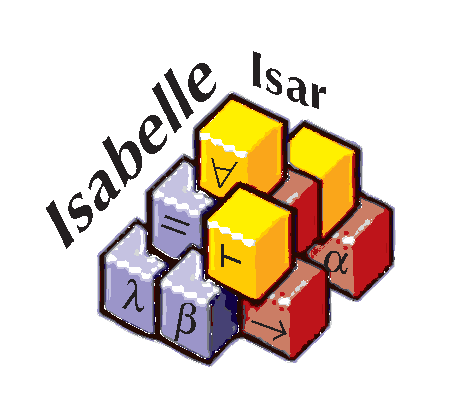
\includegraphics[scale=0.5]{isabelle_isar}
  \\[4ex] The Isabelle/Isar Implementation}
\author{\emph{Makarius Wenzel}  \\[3ex]
  With Contributions by
  Stefan Berghofer, \\
  Florian Haftmann
  and Larry Paulson
}

\makeindex


\begin{document}

\maketitle

\begin{abstract}
  We describe the key concepts underlying the Isabelle/Isar
  implementation, including ML references for the most important
  functions.  The aim is to give some insight into the overall system
  architecture, and provide clues on implementing applications within
  this framework.
\end{abstract}

\vspace*{2.5cm}
\begin{quote}

  {\small\em Isabelle was not designed; it evolved.  Not everyone
    likes this idea.  Specification experts rightly abhor
    trial-and-error programming.  They suggest that no one should
    write a program without first writing a complete formal
    specification. But university departments are not software houses.
    Programs like Isabelle are not products: when they have served
    their purpose, they are discarded.}

  Lawrence C. Paulson, ``Isabelle: The Next 700 Theorem Provers''

  \vspace*{1cm}

  {\small\em As I did 20 years ago, I still fervently believe that the
    only way to make software secure, reliable, and fast is to make it
    small.  Fight features.}

  Andrew S. Tanenbaum

  \vspace*{1cm}

  {\small\em One thing that UNIX does not need is more features. It is
    successful in part because it has a small number of good ideas
    that work well together. Merely adding features does not make it
    easier for users to do things --- it just makes the manual
    thicker. The right solution in the right place is always more
    effective than haphazard hacking.}

  Rob Pike and Brian W. Kernighan

  \vspace*{1cm}

  {\small\em If you look at software today, through the lens of the
    history of engineering, it's certainly engineering of a sort--but
    it's the kind of engineering that people without the concept of
    the arch did. Most software today is very much like an Egyptian
    pyramid with millions of bricks piled on top of each other, with
    no structural integrity, but just done by brute force and
    thousands of slaves.}

  Alan Kay

\end{quote}

\thispagestyle{empty}\clearpage

\pagenumbering{roman}
\tableofcontents
\listoffigures
\clearfirst

\setcounter{chapter}{-1}

%
\begin{isabellebody}%
\def\isabellecontext{ML}%
%
\isadelimtheory
%
\endisadelimtheory
%
\isatagtheory
\isacommand{theory}\isamarkupfalse%
\ {\isachardoublequoteopen}ML{\isachardoublequoteclose}\isanewline
\isakeyword{imports}\ Base\isanewline
\isakeyword{begin}%
\endisatagtheory
{\isafoldtheory}%
%
\isadelimtheory
%
\endisadelimtheory
%
\isamarkupchapter{Isabelle/ML%
}
\isamarkuptrue%
%
\begin{isamarkuptext}%
Isabelle/ML is best understood as a certain culture based on
  Standard ML.  Thus it is not a new programming language, but a
  certain way to use SML at an advanced level within the Isabelle
  environment.  This covers a variety of aspects that are geared
  towards an efficient and robust platform for applications of formal
  logic with fully foundational proof construction --- according to
  the well-known \emph{LCF principle}.  There is specific
  infrastructure with library modules to address the needs of this
  difficult task.  For example, the raw parallel programming model of
  Poly/ML is presented as considerably more abstract concept of
  \emph{future values}, which is then used to augment the inference
  kernel, proof interpreter, and theory loader accordingly.

  The main aspects of Isabelle/ML are introduced below.  These
  first-hand explanations should help to understand how proper
  Isabelle/ML is to be read and written, and to get access to the
  wealth of experience that is expressed in the source text and its
  history of changes.\footnote{See
  \url{http://isabelle.in.tum.de/repos/isabelle} for the full
  Mercurial history.  There are symbolic tags to refer to official
  Isabelle releases, as opposed to arbitrary \emph{tip} versions that
  merely reflect snapshots that are never really up-to-date.}%
\end{isamarkuptext}%
\isamarkuptrue%
%
\isamarkupsection{Style and orthography%
}
\isamarkuptrue%
%
\begin{isamarkuptext}%
The sources of Isabelle/Isar are optimized for
  \emph{readability} and \emph{maintainability}.  The main purpose is
  to tell an informed reader what is really going on and how things
  really work.  This is a non-trivial aim, but it is supported by a
  certain style of writing Isabelle/ML that has emerged from long
  years of system development.\footnote{See also the interesting style
  guide for OCaml
  \url{http://caml.inria.fr/resources/doc/guides/guidelines.en.html}
  which shares many of our means and ends.}

  The main principle behind any coding style is \emph{consistency}.
  For a single author of a small program this merely means ``choose
  your style and stick to it''.  A complex project like Isabelle, with
  long years of development and different contributors, requires more
  standardization.  A coding style that is changed every few years or
  with every new contributor is no style at all, because consistency
  is quickly lost.  Global consistency is hard to achieve, though.
  Nonetheless, one should always strive at least for local consistency
  of modules and sub-systems, without deviating from some general
  principles how to write Isabelle/ML.

  In a sense, good coding style is like an \emph{orthography} for the
  sources: it helps to read quickly over the text and see through the
  main points, without getting distracted by accidental presentation
  of free-style code.%
\end{isamarkuptext}%
\isamarkuptrue%
%
\isamarkupsubsection{Header and sectioning%
}
\isamarkuptrue%
%
\begin{isamarkuptext}%
Isabelle source files have a certain standardized header
  format (with precise spacing) that follows ancient traditions
  reaching back to the earliest versions of the system by Larry
  Paulson.  See \hyperlink{file.~~/src/Pure/thm.ML}{\mbox{\isa{\isatt{{\isachartilde}{\isachartilde}{\isacharslash}src{\isacharslash}Pure{\isacharslash}thm{\isachardot}ML}}}}, for example.

  The header includes at least \verb|Title| and \verb|Author| entries, followed by a prose description of the purpose of
  the module.  The latter can range from a single line to several
  paragraphs of explanations.

  The rest of the file is divided into sections, subsections,
  subsubsections, paragraphs etc.\ using a simple layout via ML
  comments as follows.

\begin{verbatim}
(*** section ***)

(** subsection **)

(* subsubsection *)

(*short paragraph*)

(*
  long paragraph,
  with more text
*)
\end{verbatim}

  As in regular typography, there is some extra space \emph{before}
  section headings that are adjacent to plain text (not other headings
  as in the example above).

  \medskip The precise wording of the prose text given in these
  headings is chosen carefully to introduce the main theme of the
  subsequent formal ML text.%
\end{isamarkuptext}%
\isamarkuptrue%
%
\isamarkupsubsection{Naming conventions%
}
\isamarkuptrue%
%
\begin{isamarkuptext}%
Since ML is the primary medium to express the meaning of the
  source text, naming of ML entities requires special care.

  \paragraph{Notation.}  A name consists of 1--3 \emph{words} (rarely
  4, but not more) that are separated by underscore.  There are three
  variants concerning upper or lower case letters, which are used for
  certain ML categories as follows:

  \medskip
  \begin{tabular}{lll}
  variant & example & ML categories \\\hline
  lower-case & \verb|foo_bar| & values, types, record fields \\
  capitalized & \verb|Foo_Bar| & datatype constructors, structures, functors \\
  upper-case & \verb|FOO_BAR| & special values, exception constructors, signatures \\
  \end{tabular}
  \medskip

  For historical reasons, many capitalized names omit underscores,
  e.g.\ old-style \verb|FooBar| instead of \verb|Foo_Bar|.
  Genuine mixed-case names are \emph{not} used, bacause clear division
  of words is essential for readability.\footnote{Camel-case was
  invented to workaround the lack of underscore in some early
  non-ASCII character sets.  Later it became habitual in some language
  communities that are now strong in numbers.}

  A single (capital) character does not count as ``word'' in this
  respect: some Isabelle/ML names are suffixed by extra markers like
  this: \verb|foo_barT|.

  Name variants are produced by adding 1--3 primes, e.g.\ \verb|foo'|, \verb|foo''|, or \verb|foo'''|, but not \verb|foo''''| or more.  Decimal digits scale better to larger numbers,
  e.g.\ \verb|foo0|, \verb|foo1|, \verb|foo42|.

  \paragraph{Scopes.}  Apart from very basic library modules, ML
  structures are not ``opened'', but names are referenced with
  explicit qualification, as in \verb|Syntax.string_of_term| for
  example.  When devising names for structures and their components it
  is important aim at eye-catching compositions of both parts, because
  this is how they are seen in the sources and documentation.  For the
  same reasons, aliases of well-known library functions should be
  avoided.

  Local names of function abstraction or case/let bindings are
  typically shorter, sometimes using only rudiments of ``words'',
  while still avoiding cryptic shorthands.  An auxiliary function
  called \verb|helper|, \verb|aux|, or \verb|f| is
  considered bad style.

  Example:

  \begin{verbatim}
  (* RIGHT *)

  fun print_foo ctxt foo =
    let
      fun print t = ... Syntax.string_of_term ctxt t ...
    in ... end;


  (* RIGHT *)

  fun print_foo ctxt foo =
    let
      val string_of_term = Syntax.string_of_term ctxt;
      fun print t = ... string_of_term t ...
    in ... end;


  (* WRONG *)

  val string_of_term = Syntax.string_of_term;

  fun print_foo ctxt foo =
    let
      fun aux t = ... string_of_term ctxt t ...
    in ... end;

  \end{verbatim}


  \paragraph{Specific conventions.} Here are some specific name forms
  that occur frequently in the sources.

  \begin{itemize}

  \item A function that maps \verb|foo| to \verb|bar| is
  called \verb|foo_to_bar| or \verb|bar_of_foo| (never
  \verb|foo2bar|, \verb|bar_from_foo|, \verb|bar_for_foo|, or \verb|bar4foo|).

  \item The name component \verb|legacy| means that the operation
  is about to be discontinued soon.

  \item The name component \verb|old| means that this is historic
  material that might disappear at some later stage.

  \item The name component \verb|global| means that this works
  with the background theory instead of the regular local context
  (\secref{sec:context}), sometimes for historical reasons, sometimes
  due a genuine lack of locality of the concept involved, sometimes as
  a fall-back for the lack of a proper context in the application
  code.  Whenever there is a non-global variant available, the
  application should be migrated to use it with a proper local
  context.

  \item Variables of the main context types of the Isabelle/Isar
  framework (\secref{sec:context} and \chref{ch:local-theory}) have
  firm naming conventions as follows:

  \begin{itemize}

  \item theories are called \verb|thy|, rarely \verb|theory|
  (never \verb|thry|)

  \item proof contexts are called \verb|ctxt|, rarely \verb|context| (never \verb|ctx|)

  \item generic contexts are called \verb|context|, rarely
  \verb|ctxt|

  \item local theories are called \verb|lthy|, except for local
  theories that are treated as proof context (which is a semantic
  super-type)

  \end{itemize}

  Variations with primed or decimal numbers are always possible, as
  well as sematic prefixes like \verb|foo_thy| or \verb|bar_ctxt|, but the base conventions above need to be preserved.
  This allows to visualize the their data flow via plain regular
  expressions in the editor.

  \item The main logical entities (\secref{ch:logic}) have established
  naming convention as follows:

  \begin{itemize}

  \item sorts are called \verb|S|

  \item types are called \verb|T|, \verb|U|, or \verb|ty| (never \verb|t|)

  \item terms are called \verb|t|, \verb|u|, or \verb|tm| (never \verb|trm|)

  \item certified types are called \verb|cT|, rarely \verb|T|, with variants as for types

  \item certified terms are called \verb|ct|, rarely \verb|t|, with variants as for terms

  \item theorems are called \verb|th|, or \verb|thm|

  \end{itemize}

  Proper semantic names override these conventions completely.  For
  example, the left-hand side of an equation (as a term) can be called
  \verb|lhs| (not \verb|lhs_tm|).  Or a term that is known
  to be a variable can be called \verb|v| or \verb|x|.

  \end{itemize}%
\end{isamarkuptext}%
\isamarkuptrue%
%
\isamarkupsubsection{General source layout%
}
\isamarkuptrue%
%
\begin{isamarkuptext}%
The general Isabelle/ML source layout imitates regular
  type-setting to some extent, augmented by the requirements for
  deeply nested expressions that are commonplace in functional
  programming.

  \paragraph{Line length} is 80 characters according to ancient
  standards, but we allow as much as 100 characters (not
  more).\footnote{Readability requires to keep the beginning of a line
  in view while watching its end.  Modern wide-screen displays do not
  change the way how the human brain works.  Sources also need to be
  printable on plain paper with reasonable font-size.} The extra 20
  characters acknowledge the space requirements due to qualified
  library references in Isabelle/ML.

  \paragraph{White-space} is used to emphasize the structure of
  expressions, following mostly standard conventions for mathematical
  typesetting, as can be seen in plain {\TeX} or {\LaTeX}.  This
  defines positioning of spaces for parentheses, punctuation, and
  infixes as illustrated here:

  \begin{verbatim}
  val x = y + z * (a + b);
  val pair = (a, b);
  val record = {foo = 1, bar = 2};
  \end{verbatim}

  Lines are normally broken \emph{after} an infix operator or
  punctuation character.  For example:

  \begin{verbatim}
  val x =
    a +
    b +
    c;

  val tuple =
   (a,
    b,
    c);
  \end{verbatim}

  Some special infixes (e.g.\ \verb||\verb,|,\verb|>|) work better at the
  start of the line, but punctuation is always at the end.

  Function application follows the tradition of \isa{{\isasymlambda}}-calculus,
  not informal mathematics.  For example: \verb|f a b| for a
  curried function, or \verb|g (a, b)| for a tupled function.
  Note that the space between \verb|g| and the pair \verb|(a, b)| follows the important principle of
  \emph{compositionality}: the layout of \verb|g p| does not
  change when \verb|p| is refined to the concrete pair
  \verb|(a, b)|.

  \paragraph{Indentation} uses plain spaces, never hard
  tabulators.\footnote{Tabulators were invented to move the carriage
  of a type-writer to certain predefined positions.  In software they
  could be used as a primitive run-length compression of consecutive
  spaces, but the precise result would depend on non-standardized
  editor configuration.}

  Each level of nesting is indented by 2 spaces, sometimes 1, very
  rarely 4, never 8 or any other odd number.

  Indentation follows a simple logical format that only depends on the
  nesting depth, not the accidental length of the text that initiates
  a level of nesting.  Example:

  \begin{verbatim}
  (* RIGHT *)

  if b then
    expr1_part1
    expr1_part2
  else
    expr2_part1
    expr2_part2


  (* WRONG *)

  if b then expr1_part1
            expr1_part2
  else expr2_part1
       expr2_part2
  \end{verbatim}

  The second form has many problems: it assumes a fixed-width font
  when viewing the sources, it uses more space on the line and thus
  makes it hard to observe its strict length limit (working against
  \emph{readability}), it requires extra editing to adapt the layout
  to changes of the initial text (working against
  \emph{maintainability}) etc.

  \medskip For similar reasons, any kind of two-dimensional or tabular
  layouts, ASCII-art with lines or boxes of asterisks etc.\ should be
  avoided.

  \paragraph{Complex expressions} that consist of multi-clausal
  function definitions, \verb|handle|, \verb|case|,
  \verb|let| (and combinations) require special attention.  The
  syntax of Standard ML is quite ambitious and admits a lot of
  variance that can distort the meaning of the text.

  Clauses of \verb|fun|, \verb|fn|, \verb|handle|,
  \verb|case| get extra indentation to indicate the nesting
  clearly.  Example:

  \begin{verbatim}
  (* RIGHT *)

  fun foo p1 =
        expr1
    | foo p2 =
        expr2


  (* WRONG *)

  fun foo p1 =
    expr1
    | foo p2 =
    expr2
  \end{verbatim}

  Body expressions consisting of \verb|case| or \verb|let|
  require care to maintain compositionality, to prevent loss of
  logical indentation where it is especially important to see the
  structure of the text.  Example:

  \begin{verbatim}
  (* RIGHT *)

  fun foo p1 =
        (case e of
          q1 => ...
        | q2 => ...)
    | foo p2 =
        let
          ...
        in
          ...
        end


  (* WRONG *)

  fun foo p1 = case e of
      q1 => ...
    | q2 => ...
    | foo p2 =
    let
      ...
    in
      ...
    end
  \end{verbatim}

  Extra parentheses around \verb|case| expressions are optional,
  but help to analyse the nesting based on character matching in the
  editor.

  \medskip There are two main exceptions to the overall principle of
  compositionality in the layout of complex expressions.

  \begin{enumerate}

  \item \verb|if| expressions are iterated as if there would be
  a multi-branch conditional in SML, e.g.

  \begin{verbatim}
  (* RIGHT *)

  if b1 then e1
  else if b2 then e2
  else e3
  \end{verbatim}

  \item \verb|fn| abstractions are often layed-out as if they
  would lack any structure by themselves.  This traditional form is
  motivated by the possibility to shift function arguments back and
  forth wrt.\ additional combinators.  Example:

  \begin{verbatim}
  (* RIGHT *)

  fun foo x y = fold (fn z =>
    expr)
  \end{verbatim}

  Here the visual appearance is that of three arguments \verb|x|,
  \verb|y|, \verb|z|.

  \end{enumerate}

  Such weakly structured layout should be use with great care.  Here
  is a counter-example involving \verb|let| expressions:

  \begin{verbatim}
  (* WRONG *)

  fun foo x = let
      val y = ...
    in ... end

  fun foo x =
  let
    val y = ...
  in ... end
  \end{verbatim}

  \medskip In general the source layout is meant to emphasize the
  structure of complex language expressions, not to pretend that SML
  had a completely different syntax (say that of Haskell or Java).%
\end{isamarkuptext}%
\isamarkuptrue%
%
\isamarkupsection{SML embedded into Isabelle/Isar%
}
\isamarkuptrue%
%
\begin{isamarkuptext}%
ML and Isar are intertwined via an open-ended bootstrap
  process that provides more and more programming facilities and
  logical content in an alternating manner.  Bootstrapping starts from
  the raw environment of existing implementations of Standard ML
  (mainly Poly/ML, but also SML/NJ).

  Isabelle/Pure marks the point where the original ML toplevel is
  superseded by the Isar toplevel that maintains a uniform context for
  arbitrary ML values (see also \secref{sec:context}).  This formal
  environment holds ML compiler bindings, logical entities, and many
  other things.  Raw SML is never encountered again after the initial
  bootstrap of Isabelle/Pure.

  Object-logics like Isabelle/HOL are built within the
  Isabelle/ML/Isar environment by introducing suitable theories with
  associated ML modules, either inlined or as separate files.  Thus
  Isabelle/HOL is defined as a regular user-space application within
  the Isabelle framework.  Further add-on tools can be implemented in
  ML within the Isar context in the same manner: ML is part of the
  standard repertoire of Isabelle, and there is no distinction between
  ``user'' and ``developer'' in this respect.%
\end{isamarkuptext}%
\isamarkuptrue%
%
\isamarkupsubsection{Isar ML commands%
}
\isamarkuptrue%
%
\begin{isamarkuptext}%
The primary Isar source language provides facilities to ``open
  a window'' to the underlying ML compiler.  Especially see the Isar
  commands \indexref{}{command}{use}\hyperlink{command.use}{\mbox{\isa{\isacommand{use}}}} and \indexref{}{command}{ML}\hyperlink{command.ML}{\mbox{\isa{\isacommand{ML}}}}: both work the
  same way, only the source text is provided via a file vs.\ inlined,
  respectively.  Apart from embedding ML into the main theory
  definition like that, there are many more commands that refer to ML
  source, such as \indexref{}{command}{setup}\hyperlink{command.setup}{\mbox{\isa{\isacommand{setup}}}} or \indexref{}{command}{declaration}\hyperlink{command.declaration}{\mbox{\isa{\isacommand{declaration}}}}.
  Even more fine-grained embedding of ML into Isar is encountered in
  the proof method \indexref{}{method}{tactic}\hyperlink{method.tactic}{\mbox{\isa{tactic}}}, which refines the pending
  goal state via a given expression of type \verb|tactic|.%
\end{isamarkuptext}%
\isamarkuptrue%
%
\isadelimmlex
%
\endisadelimmlex
%
\isatagmlex
%
\begin{isamarkuptext}%
The following artificial example demonstrates some ML
  toplevel declarations within the implicit Isar theory context.  This
  is regular functional programming without referring to logical
  entities yet.%
\end{isamarkuptext}%
\isamarkuptrue%
%
\endisatagmlex
{\isafoldmlex}%
%
\isadelimmlex
%
\endisadelimmlex
%
\isadelimML
%
\endisadelimML
%
\isatagML
\isacommand{ML}\isamarkupfalse%
\ {\isacharverbatimopen}\isanewline
\ \ fun\ factorial\ {\isadigit{0}}\ {\isacharequal}\ {\isadigit{1}}\isanewline
\ \ \ \ {\isacharbar}\ factorial\ n\ {\isacharequal}\ n\ {\isacharasterisk}\ factorial\ {\isacharparenleft}n\ {\isacharminus}\ {\isadigit{1}}{\isacharparenright}\isanewline
{\isacharverbatimclose}%
\endisatagML
{\isafoldML}%
%
\isadelimML
%
\endisadelimML
%
\begin{isamarkuptext}%
Here the ML environment is already managed by Isabelle, i.e.\
  the \verb|factorial| function is not yet accessible in the preceding
  paragraph, nor in a different theory that is independent from the
  current one in the import hierarchy.

  Removing the above ML declaration from the source text will remove
  any trace of this definition as expected.  The Isabelle/ML toplevel
  environment is managed in a \emph{stateless} way: unlike the raw ML
  toplevel there are no global side-effects involved
  here.\footnote{Such a stateless compilation environment is also a
  prerequisite for robust parallel compilation within independent
  nodes of the implicit theory development graph.}

  \medskip The next example shows how to embed ML into Isar proofs, using
 \indexref{}{command}{ML\_prf}\hyperlink{command.ML-prf}{\mbox{\isa{\isacommand{ML{\isacharunderscore}prf}}}} instead of Instead of \indexref{}{command}{ML}\hyperlink{command.ML}{\mbox{\isa{\isacommand{ML}}}}.
  As illustrated below, the effect on the ML environment is local to
  the whole proof body, ignoring the block structure.%
\end{isamarkuptext}%
\isamarkuptrue%
\isacommand{example{\isacharunderscore}proof}\isamarkupfalse%
\isanewline
%
\isadelimML
\ \ %
\endisadelimML
%
\isatagML
\isacommand{ML{\isacharunderscore}prf}\isamarkupfalse%
\ {\isacharverbatimopen}\ val\ a\ {\isacharequal}\ {\isadigit{1}}\ {\isacharverbatimclose}\isanewline
\ \ \isacommand{{\isacharbraceleft}}\isamarkupfalse%
\isanewline
\ \ \ \ \isacommand{ML{\isacharunderscore}prf}\isamarkupfalse%
\ {\isacharverbatimopen}\ val\ b\ {\isacharequal}\ a\ {\isacharplus}\ {\isadigit{1}}\ {\isacharverbatimclose}\isanewline
\ \ \isacommand{{\isacharbraceright}}\isamarkupfalse%
\ %
\isamarkupcmt{Isar block structure ignored by ML environment%
}
\isanewline
\ \ \isacommand{ML{\isacharunderscore}prf}\isamarkupfalse%
\ {\isacharverbatimopen}\ val\ c\ {\isacharequal}\ b\ {\isacharplus}\ {\isadigit{1}}\ {\isacharverbatimclose}\isanewline
\isacommand{qed}\isamarkupfalse%
%
\endisatagML
{\isafoldML}%
%
\isadelimML
%
\endisadelimML
%
\begin{isamarkuptext}%
By side-stepping the normal scoping rules for Isar proof
  blocks, embedded ML code can refer to the different contexts and
  manipulate corresponding entities, e.g.\ export a fact from a block
  context.

  \medskip Two further ML commands are useful in certain situations:
  \indexref{}{command}{ML\_val}\hyperlink{command.ML-val}{\mbox{\isa{\isacommand{ML{\isacharunderscore}val}}}} and \indexref{}{command}{ML\_command}\hyperlink{command.ML-command}{\mbox{\isa{\isacommand{ML{\isacharunderscore}command}}}} are
  \emph{diagnostic} in the sense that there is no effect on the
  underlying environment, and can thus used anywhere (even outside a
  theory).  The examples below produce long strings of digits by
  invoking \verb|factorial|: \hyperlink{command.ML-val}{\mbox{\isa{\isacommand{ML{\isacharunderscore}val}}}} already takes care of
  printing the ML toplevel result, but \hyperlink{command.ML-command}{\mbox{\isa{\isacommand{ML{\isacharunderscore}command}}}} is silent
  so we produce an explicit output message.%
\end{isamarkuptext}%
\isamarkuptrue%
%
\isadelimML
%
\endisadelimML
%
\isatagML
\isacommand{ML{\isacharunderscore}val}\isamarkupfalse%
\ {\isacharverbatimopen}\ factorial\ {\isadigit{1}}{\isadigit{0}}{\isadigit{0}}\ {\isacharverbatimclose}\isanewline
\isacommand{ML{\isacharunderscore}command}\isamarkupfalse%
\ {\isacharverbatimopen}\ writeln\ {\isacharparenleft}string{\isacharunderscore}of{\isacharunderscore}int\ {\isacharparenleft}factorial\ {\isadigit{1}}{\isadigit{0}}{\isadigit{0}}{\isacharparenright}{\isacharparenright}\ {\isacharverbatimclose}%
\endisatagML
{\isafoldML}%
%
\isadelimML
%
\endisadelimML
\isanewline
\isanewline
\isacommand{example{\isacharunderscore}proof}\isamarkupfalse%
\isanewline
%
\isadelimML
\ \ %
\endisadelimML
%
\isatagML
\isacommand{ML{\isacharunderscore}val}\isamarkupfalse%
\ {\isacharverbatimopen}\ factorial\ {\isadigit{1}}{\isadigit{0}}{\isadigit{0}}\ {\isacharverbatimclose}\ \ \isanewline
\ \ \isacommand{ML{\isacharunderscore}command}\isamarkupfalse%
\ {\isacharverbatimopen}\ writeln\ {\isacharparenleft}string{\isacharunderscore}of{\isacharunderscore}int\ {\isacharparenleft}factorial\ {\isadigit{1}}{\isadigit{0}}{\isadigit{0}}{\isacharparenright}{\isacharparenright}\ {\isacharverbatimclose}%
\endisatagML
{\isafoldML}%
%
\isadelimML
\isanewline
%
\endisadelimML
%
\isadelimproof
%
\endisadelimproof
%
\isatagproof
\isacommand{qed}\isamarkupfalse%
%
\endisatagproof
{\isafoldproof}%
%
\isadelimproof
%
\endisadelimproof
%
\isamarkupsubsection{Compile-time context%
}
\isamarkuptrue%
%
\begin{isamarkuptext}%
Whenever the ML compiler is invoked within Isabelle/Isar, the
  formal context is passed as a thread-local reference variable.  Thus
  ML code may access the theory context during compilation, by reading
  or writing the (local) theory under construction.  Note that such
  direct access to the compile-time context is rare.  In practice it
  is typically done via some derived ML functions instead.%
\end{isamarkuptext}%
\isamarkuptrue%
%
\isadelimmlref
%
\endisadelimmlref
%
\isatagmlref
%
\begin{isamarkuptext}%
\begin{mldecls}
  \indexdef{}{ML}{ML\_Context.the\_generic\_context}\verb|ML_Context.the_generic_context: unit -> Context.generic| \\
  \indexdef{}{ML}{Context.$>$$>$}\verb|Context.>> : (Context.generic -> Context.generic) -> unit| \\
  \indexdef{}{ML}{bind\_thms}\verb|bind_thms: string * thm list -> unit| \\
  \indexdef{}{ML}{bind\_thm}\verb|bind_thm: string * thm -> unit| \\
  \end{mldecls}

  \begin{description}

  \item \verb|ML_Context.the_generic_context ()| refers to the theory
  context of the ML toplevel --- at compile time.  ML code needs to
  take care to refer to \verb|ML_Context.the_generic_context ()|
  correctly.  Recall that evaluation of a function body is delayed
  until actual run-time.

  \item \verb|Context.>>|~\isa{f} applies context transformation
  \isa{f} to the implicit context of the ML toplevel.

  \item \verb|bind_thms|~\isa{{\isacharparenleft}name{\isacharcomma}\ thms{\isacharparenright}} stores a list of
  theorems produced in ML both in the (global) theory context and the
  ML toplevel, associating it with the provided name.  Theorems are
  put into a global ``standard'' format before being stored.

  \item \verb|bind_thm| is similar to \verb|bind_thms| but refers to a
  singleton fact.

  \end{description}

  It is important to note that the above functions are really
  restricted to the compile time, even though the ML compiler is
  invoked at run-time.  The majority of ML code either uses static
  antiquotations (\secref{sec:ML-antiq}) or refers to the theory or
  proof context at run-time, by explicit functional abstraction.%
\end{isamarkuptext}%
\isamarkuptrue%
%
\endisatagmlref
{\isafoldmlref}%
%
\isadelimmlref
%
\endisadelimmlref
%
\isamarkupsubsection{Antiquotations \label{sec:ML-antiq}%
}
\isamarkuptrue%
%
\begin{isamarkuptext}%
A very important consequence of embedding SML into Isar is the
  concept of \emph{ML antiquotation}.  The standard token language of
  ML is augmented by special syntactic entities of the following form:

  \indexouternonterm{antiquote}
  \begin{rail}
  antiquote: atsign lbrace nameref args rbrace | lbracesym | rbracesym
  ;
  \end{rail}

  Here \hyperlink{syntax.nameref}{\mbox{\isa{nameref}}} and \hyperlink{syntax.args}{\mbox{\isa{args}}} are regular outer syntax
  categories \cite{isabelle-isar-ref}.  Attributes and proof methods
  use similar syntax.

  \medskip A regular antiquotation \isa{{\isacharat}{\isacharbraceleft}name\ args{\isacharbraceright}} processes
  its arguments by the usual means of the Isar source language, and
  produces corresponding ML source text, either as literal
  \emph{inline} text (e.g. \isa{{\isacharat}{\isacharbraceleft}term\ t{\isacharbraceright}}) or abstract
  \emph{value} (e.g. \isa{{\isacharat}{\isacharbraceleft}thm\ th{\isacharbraceright}}).  This pre-compilation
  scheme allows to refer to formal entities in a robust manner, with
  proper static scoping and with some degree of logical checking of
  small portions of the code.

  Special antiquotations like \isa{{\isacharat}{\isacharbraceleft}let\ {\isasymdots}{\isacharbraceright}} or \isa{{\isacharat}{\isacharbraceleft}note\ {\isasymdots}{\isacharbraceright}} augment the compilation context without generating code.  The
  non-ASCII braces \isa{{\isasymlbrace}} and \isa{{\isasymrbrace}} allow to delimit the
  effect by introducing local blocks within the pre-compilation
  environment.

  \medskip See also \cite{Wenzel-Chaieb:2007b} for a broader
  perspective on Isabelle/ML antiquotations.%
\end{isamarkuptext}%
\isamarkuptrue%
%
\isadelimmlantiq
%
\endisadelimmlantiq
%
\isatagmlantiq
%
\begin{isamarkuptext}%
\begin{matharray}{rcl}
  \indexdef{}{ML antiquotation}{let}\hypertarget{ML antiquotation.let}{\hyperlink{ML antiquotation.let}{\mbox{\isa{let}}}} & : & \isa{ML{\isacharunderscore}antiquotation} \\
  \indexdef{}{ML antiquotation}{note}\hypertarget{ML antiquotation.note}{\hyperlink{ML antiquotation.note}{\mbox{\isa{note}}}} & : & \isa{ML{\isacharunderscore}antiquotation} \\
  \end{matharray}

  \begin{rail}
  'let' ((term + 'and') '=' term + 'and')
  ;

  'note' (thmdef? thmrefs + 'and')
  ;
  \end{rail}

  \begin{description}

  \item \isa{{\isacharat}{\isacharbraceleft}let\ p\ {\isacharequal}\ t{\isacharbraceright}} binds schematic variables in the
  pattern \isa{p} by higher-order matching against the term \isa{t}.  This is analogous to the regular \indexref{}{command}{let}\hyperlink{command.let}{\mbox{\isa{\isacommand{let}}}} command
  in the Isar proof language.  The pre-compilation environment is
  augmented by auxiliary term bindings, without emitting ML source.

  \item \isa{{\isacharat}{\isacharbraceleft}note\ a\ {\isacharequal}\ b\isactrlsub {\isadigit{1}}\ {\isasymdots}\ b\isactrlsub n{\isacharbraceright}} recalls existing facts \isa{b\isactrlsub {\isadigit{1}}{\isacharcomma}\ {\isasymdots}{\isacharcomma}\ b\isactrlsub n}, binding the result as \isa{a}.  This is analogous to
  the regular \indexref{}{command}{note}\hyperlink{command.note}{\mbox{\isa{\isacommand{note}}}} command in the Isar proof language.
  The pre-compilation environment is augmented by auxiliary fact
  bindings, without emitting ML source.

  \end{description}%
\end{isamarkuptext}%
\isamarkuptrue%
%
\endisatagmlantiq
{\isafoldmlantiq}%
%
\isadelimmlantiq
%
\endisadelimmlantiq
%
\isadelimmlex
%
\endisadelimmlex
%
\isatagmlex
%
\begin{isamarkuptext}%
The following artificial example gives some impression
  about the antiquotation elements introduced so far, together with
  the important \isa{{\isacharat}{\isacharbraceleft}thm{\isacharbraceright}} antiquotation defined later.%
\end{isamarkuptext}%
\isamarkuptrue%
%
\endisatagmlex
{\isafoldmlex}%
%
\isadelimmlex
%
\endisadelimmlex
%
\isadelimML
%
\endisadelimML
%
\isatagML
\isacommand{ML}\isamarkupfalse%
\ {\isacharverbatimopen}\isanewline
\ \ {\isaantiqopen}\isanewline
\ \ \ \ %
\isaantiq
let\ {\isacharquery}t\ {\isacharequal}\ my{\isacharunderscore}term%
\endisaantiq
\isanewline
\ \ \ \ %
\isaantiq
note\ my{\isacharunderscore}refl\ {\isacharequal}\ reflexive\ {\isacharbrackleft}of\ {\isacharquery}t{\isacharbrackright}%
\endisaantiq
\isanewline
\ \ \ \ fun\ foo\ th\ {\isacharequal}\ Thm{\isachardot}transitive\ th\ %
\isaantiq
thm\ my{\isacharunderscore}refl%
\endisaantiq
\isanewline
\ \ {\isaantiqclose}\isanewline
{\isacharverbatimclose}%
\endisatagML
{\isafoldML}%
%
\isadelimML
%
\endisadelimML
%
\begin{isamarkuptext}%
The extra block delimiters do not affect the compiled code
  itself, i.e.\ function \verb|foo| is available in the present context
  of this paragraph.%
\end{isamarkuptext}%
\isamarkuptrue%
%
\isamarkupsection{Canonical argument order \label{sec:canonical-argument-order}%
}
\isamarkuptrue%
%
\begin{isamarkuptext}%
Standard ML is a language in the tradition of \isa{{\isasymlambda}}-calculus and \emph{higher-order functional programming},
  similar to OCaml, Haskell, or Isabelle/Pure and HOL as logical
  languages.  Getting acquainted with the native style of representing
  functions in that setting can save a lot of extra boiler-plate of
  redundant shuffling of arguments, auxiliary abstractions etc.

  Functions are usually \emph{curried}: the idea of turning arguments
  of type \isa{{\isasymtau}\isactrlsub i} (for \isa{i\ {\isasymin}\ {\isacharbraceleft}{\isadigit{1}}{\isacharcomma}\ {\isasymdots}\ n{\isacharbraceright}}) into a result of
  type \isa{{\isasymtau}} is represented by the iterated function space
  \isa{{\isasymtau}\isactrlsub {\isadigit{1}}\ {\isasymrightarrow}\ {\isasymdots}\ {\isasymrightarrow}\ {\isasymtau}\isactrlsub n\ {\isasymrightarrow}\ {\isasymtau}}.  This is isomorphic to the well-known
  encoding via tuples \isa{{\isasymtau}\isactrlsub {\isadigit{1}}\ {\isasymtimes}\ {\isasymdots}\ {\isasymtimes}\ {\isasymtau}\isactrlsub n\ {\isasymrightarrow}\ {\isasymtau}}, but the curried
  version fits more smoothly into the basic calculus.\footnote{The
  difference is even more significant in higher-order logic, because
  the redundant tuple structure needs to be accommodated by formal
  reasoning.}

  Currying gives some flexiblity due to \emph{partial application}.  A
  function \isa{f{\isacharcolon}\ {\isasymtau}\isactrlsub {\isadigit{1}}\ {\isasymrightarrow}\ {\isasymtau}\isactrlbsub {\isadigit{2}}\isactrlesub \ {\isasymrightarrow}\ {\isasymtau}} can be applied to \isa{x{\isacharcolon}\ {\isasymtau}\isactrlsub {\isadigit{1}}}
  and the remaining \isa{{\isacharparenleft}f\ x{\isacharparenright}{\isacharcolon}\ {\isasymtau}\isactrlsub {\isadigit{2}}\ {\isasymrightarrow}\ {\isasymtau}} passed to another function
  etc.  How well this works in practice depends on the order of
  arguments.  In the worst case, arguments are arranged erratically,
  and using a function in a certain situation always requires some
  glue code.  Thus we would get exponentially many oppurtunities to
  decorate the code with meaningless permutations of arguments.

  This can be avoided by \emph{canonical argument order}, which
  observes certain standard patterns and minimizes adhoc permutations
  in their application.  In Isabelle/ML, large portions text can be
  written without ever using \isa{swap{\isacharcolon}\ {\isasymalpha}\ {\isasymtimes}\ {\isasymbeta}\ {\isasymrightarrow}\ {\isasymbeta}\ {\isasymtimes}\ {\isasymalpha}}, or the
  combinator \isa{C{\isacharcolon}\ {\isacharparenleft}{\isasymalpha}\ {\isasymrightarrow}\ {\isasymbeta}\ {\isasymrightarrow}\ {\isasymgamma}{\isacharparenright}\ {\isasymrightarrow}\ {\isacharparenleft}{\isasymbeta}\ {\isasymrightarrow}\ {\isasymalpha}\ {\isasymrightarrow}\ {\isasymgamma}{\isacharparenright}} that is not even
  defined in our library.

  \medskip The basic idea is that arguments that vary less are moved
  further to the left than those that vary more.  Two particularly
  important categories of functions are \emph{selectors} and
  \emph{updates}.

  The subsequent scheme is based on a hypothetical set-like container
  of type \isa{{\isasymbeta}} that manages elements of type \isa{{\isasymalpha}}.  Both
  the names and types of the associated operations are canonical for
  Isabelle/ML.

  \medskip
  \begin{tabular}{ll}
  kind & canonical name and type \\\hline
  selector & \isa{member{\isacharcolon}\ {\isasymbeta}\ {\isasymrightarrow}\ {\isasymalpha}\ {\isasymrightarrow}\ bool} \\
  update & \isa{insert{\isacharcolon}\ {\isasymalpha}\ {\isasymrightarrow}\ {\isasymbeta}\ {\isasymrightarrow}\ {\isasymbeta}} \\
  \end{tabular}
  \medskip

  Given a container \isa{B{\isacharcolon}\ {\isasymbeta}}, the partially applied \isa{member\ B} is a predicate over elements \isa{{\isasymalpha}\ {\isasymrightarrow}\ bool}, and
  thus represents the intended denotation directly.  It is customary
  to pass the abstract predicate to further operations, not the
  concrete container.  The argument order makes it easy to use other
  combinators: \isa{forall\ {\isacharparenleft}member\ B{\isacharparenright}\ list} will check a list of
  elements for membership in \isa{B} etc. Often the explicit
  \isa{list} is pointless and can be contracted to \isa{forall\ {\isacharparenleft}member\ B{\isacharparenright}} to get directly a predicate again.

  In contrast, an update operation varies the container, so it moves
  to the right: \isa{insert\ a} is a function \isa{{\isasymbeta}\ {\isasymrightarrow}\ {\isasymbeta}} to
  insert a value \isa{a}.  These can be composed naturally as
  \isa{insert\ c\ {\isasymcirc}\ insert\ b\ {\isasymcirc}\ insert\ a}.  The slightly awkward
  inversion if the composition order is due to conventional
  mathematical notation, which can be easily amended as explained
  below.%
\end{isamarkuptext}%
\isamarkuptrue%
%
\isamarkupsubsection{Forward application and composition%
}
\isamarkuptrue%
%
\begin{isamarkuptext}%
Regular function application and infix notation works best for
  relatively deeply structured expressions, e.g.\ \isa{h\ {\isacharparenleft}f\ x\ y\ {\isacharplus}\ g\ z{\isacharparenright}}.  The important special case of \emph{linear transformation}
  applies a cascade of functions \isa{f\isactrlsub n\ {\isacharparenleft}{\isasymdots}\ {\isacharparenleft}f\isactrlsub {\isadigit{1}}\ x{\isacharparenright}{\isacharparenright}}.  This
  becomes hard to read and maintain if the functions are themselves
  given as complex expressions.  The notation can be significantly
  improved by introducing \emph{forward} versions of application and
  composition as follows:

  \medskip
  \begin{tabular}{lll}
  \isa{x\ {\isacharbar}{\isachargreater}\ f} & \isa{{\isasymequiv}} & \isa{f\ x} \\
  \isa{f\ {\isacharhash}{\isachargreater}\ g} & \isa{{\isasymequiv}} & \isa{x\ {\isacharbar}{\isachargreater}\ f\ {\isacharbar}{\isachargreater}\ g} \\
  \end{tabular}
  \medskip

  This enables to write conveniently \isa{x\ {\isacharbar}{\isachargreater}\ f\isactrlsub {\isadigit{1}}\ {\isacharbar}{\isachargreater}\ {\isasymdots}\ {\isacharbar}{\isachargreater}\ f\isactrlsub n} or
  \isa{f\isactrlsub {\isadigit{1}}\ {\isacharhash}{\isachargreater}\ {\isasymdots}\ {\isacharhash}{\isachargreater}\ f\isactrlsub n} for its functional abstraction over \isa{x}.

  \medskip There is an additional set of combinators to accommodate
  multiple results (via pairs) that are passed on as multiple
  arguments (via currying).

  \medskip
  \begin{tabular}{lll}
  \isa{{\isacharparenleft}x{\isacharcomma}\ y{\isacharparenright}\ {\isacharbar}{\isacharminus}{\isachargreater}\ f} & \isa{{\isasymequiv}} & \isa{f\ x\ y} \\
  \isa{f\ {\isacharhash}{\isacharminus}{\isachargreater}\ g} & \isa{{\isasymequiv}} & \isa{x\ {\isacharbar}{\isachargreater}\ f\ {\isacharbar}{\isacharminus}{\isachargreater}\ g} \\
  \end{tabular}
  \medskip%
\end{isamarkuptext}%
\isamarkuptrue%
%
\isadelimmlref
%
\endisadelimmlref
%
\isatagmlref
%
\begin{isamarkuptext}%
\begin{mldecls}
  \indexdef{}{ML}{$\mid$$>$}\verb|op |\verb,|,\verb|>  : 'a * ('a -> 'b) -> 'b| \\
  \indexdef{}{ML}{$\mid$-$>$}\verb|op |\verb,|,\verb|->  : ('c * 'a) * ('c -> 'a -> 'b) -> 'b| \\
  \indexdef{}{ML}{\#$>$}\verb|op #>  : ('a -> 'b) * ('b -> 'c) -> 'a -> 'c| \\
  \indexdef{}{ML}{\#-$>$}\verb|op #->  : ('a -> 'c * 'b) * ('c -> 'b -> 'd) -> 'a -> 'd| \\
  \end{mldecls}

  %FIXME description!?%
\end{isamarkuptext}%
\isamarkuptrue%
%
\endisatagmlref
{\isafoldmlref}%
%
\isadelimmlref
%
\endisadelimmlref
%
\isamarkupsubsection{Canonical iteration%
}
\isamarkuptrue%
%
\begin{isamarkuptext}%
As explained above, a function \isa{f{\isacharcolon}\ {\isasymalpha}\ {\isasymrightarrow}\ {\isasymbeta}\ {\isasymrightarrow}\ {\isasymbeta}} can be
  understood as update on a configuration of type \isa{{\isasymbeta}},
  parametrized by arguments of type \isa{{\isasymalpha}}.  Given \isa{a{\isacharcolon}\ {\isasymalpha}}
  the partial application \isa{{\isacharparenleft}f\ a{\isacharparenright}{\isacharcolon}\ {\isasymbeta}\ {\isasymrightarrow}\ {\isasymbeta}} operates
  homogeneously on \isa{{\isasymbeta}}.  This can be iterated naturally over a
  list of parameters \isa{{\isacharbrackleft}a\isactrlsub {\isadigit{1}}{\isacharcomma}\ {\isasymdots}{\isacharcomma}\ a\isactrlsub n{\isacharbrackright}} as \isa{f\ a\isactrlsub {\isadigit{1}}\ {\isacharhash}{\isachargreater}\ {\isasymdots}\ {\isacharhash}{\isachargreater}\ f\ a\isactrlbsub n\isactrlesub \isactrlbsub \isactrlesub }.  The latter expression is again a function \isa{{\isasymbeta}\ {\isasymrightarrow}\ {\isasymbeta}}.
  It can be applied to an initial configuration \isa{b{\isacharcolon}\ {\isasymbeta}} to
  start the iteration over the given list of arguments: each \isa{a} in \isa{a\isactrlsub {\isadigit{1}}{\isacharcomma}\ {\isasymdots}{\isacharcomma}\ a\isactrlsub n} is applied consecutively by updating a
  cumulative configuration.

  The \isa{fold} combinator in Isabelle/ML lifts a function \isa{f} as above to its iterated version over a list of arguments.
  Lifting can be repeated, e.g.\ \isa{{\isacharparenleft}fold\ {\isasymcirc}\ fold{\isacharparenright}\ f} iterates
  over a list of lists as expected.

  The variant \isa{fold{\isacharunderscore}rev} works inside-out over the list of
  arguments, such that \isa{fold{\isacharunderscore}rev\ f\ {\isasymequiv}\ fold\ f\ {\isasymcirc}\ rev} holds.

  The \isa{fold{\isacharunderscore}map} combinator essentially performs \isa{fold} and \isa{map} simultaneously: each application of \isa{f} produces an updated configuration together with a side-result;
  the iteration collects all such side-results as a separate list.%
\end{isamarkuptext}%
\isamarkuptrue%
%
\isadelimmlref
%
\endisadelimmlref
%
\isatagmlref
%
\begin{isamarkuptext}%
\begin{mldecls}
  \indexdef{}{ML}{fold}\verb|fold: ('a -> 'b -> 'b) -> 'a list -> 'b -> 'b| \\
  \indexdef{}{ML}{fold\_rev}\verb|fold_rev: ('a -> 'b -> 'b) -> 'a list -> 'b -> 'b| \\
  \indexdef{}{ML}{fold\_map}\verb|fold_map: ('a -> 'b -> 'c * 'b) -> 'a list -> 'b -> 'c list * 'b| \\
  \end{mldecls}

  \begin{description}

  \item \verb|fold|~\isa{f} lifts the parametrized update function
  \isa{f} to a list of parameters.

  \item \verb|fold_rev|~\isa{f} is similar to \verb|fold|~\isa{f}, but works inside-out.

  \item \verb|fold_map|~\isa{f} lifts the parametrized update
  function \isa{f} (with side-result) to a list of parameters and
  cumulative side-results.

  \end{description}

  \begin{warn}
  The literature on functional programming provides a multitude of
  combinators called \isa{foldl}, \isa{foldr} etc.  SML97
  provides its own variations as \verb|List.foldl| and \verb|List.foldr|, while the classic Isabelle library also has the
  historic \verb|Library.foldl| and \verb|Library.foldr|.  To avoid
  further confusion, all of this should be ignored, and \verb|fold| (or
  \verb|fold_rev|) used exclusively.
  \end{warn}%
\end{isamarkuptext}%
\isamarkuptrue%
%
\endisatagmlref
{\isafoldmlref}%
%
\isadelimmlref
%
\endisadelimmlref
%
\isadelimmlex
%
\endisadelimmlex
%
\isatagmlex
%
\begin{isamarkuptext}%
The following example shows how to fill a text buffer
  incrementally by adding strings, either individually or from a given
  list.%
\end{isamarkuptext}%
\isamarkuptrue%
%
\endisatagmlex
{\isafoldmlex}%
%
\isadelimmlex
%
\endisadelimmlex
%
\isadelimML
%
\endisadelimML
%
\isatagML
\isacommand{ML}\isamarkupfalse%
\ {\isacharverbatimopen}\isanewline
\ \ val\ s\ {\isacharequal}\isanewline
\ \ \ \ Buffer{\isachardot}empty\isanewline
\ \ \ \ {\isacharbar}{\isachargreater}\ Buffer{\isachardot}add\ {\isachardoublequote}digits{\isacharcolon}\ {\isachardoublequote}\isanewline
\ \ \ \ {\isacharbar}{\isachargreater}\ fold\ {\isacharparenleft}Buffer{\isachardot}add\ o\ string{\isacharunderscore}of{\isacharunderscore}int{\isacharparenright}\ {\isacharparenleft}{\isadigit{0}}\ upto\ {\isadigit{9}}{\isacharparenright}\isanewline
\ \ \ \ {\isacharbar}{\isachargreater}\ Buffer{\isachardot}content{\isacharsemicolon}\isanewline
\isanewline
\ \ %
\isaantiq
assert%
\endisaantiq
\ {\isacharparenleft}s\ {\isacharequal}\ {\isachardoublequote}digits{\isacharcolon}\ {\isadigit{0}}{\isadigit{1}}{\isadigit{2}}{\isadigit{3}}{\isadigit{4}}{\isadigit{5}}{\isadigit{6}}{\isadigit{7}}{\isadigit{8}}{\isadigit{9}}{\isachardoublequote}{\isacharparenright}{\isacharsemicolon}\isanewline
{\isacharverbatimclose}%
\endisatagML
{\isafoldML}%
%
\isadelimML
%
\endisadelimML
%
\begin{isamarkuptext}%
Note how \verb|fold (Buffer.add o string_of_int)| above saves
  an extra \verb|map| over the given list.  This kind of peephole
  optimization reduces both the code size and the tree structures in
  memory (``deforestation''), but requires some practice to read and
  write it fluently.

  \medskip The next example elaborates the idea of canonical
  iteration, demonstrating fast accumulation of tree content using a
  text buffer.%
\end{isamarkuptext}%
\isamarkuptrue%
%
\isadelimML
%
\endisadelimML
%
\isatagML
\isacommand{ML}\isamarkupfalse%
\ {\isacharverbatimopen}\isanewline
\ \ datatype\ tree\ {\isacharequal}\ Text\ of\ string\ {\isacharbar}\ Elem\ of\ string\ {\isacharasterisk}\ tree\ list{\isacharsemicolon}\isanewline
\isanewline
\ \ fun\ slow{\isacharunderscore}content\ {\isacharparenleft}Text\ txt{\isacharparenright}\ {\isacharequal}\ txt\isanewline
\ \ \ \ {\isacharbar}\ slow{\isacharunderscore}content\ {\isacharparenleft}Elem\ {\isacharparenleft}name{\isacharcomma}\ ts{\isacharparenright}{\isacharparenright}\ {\isacharequal}\isanewline
\ \ \ \ \ \ \ \ {\isachardoublequote}{\isacharless}{\isachardoublequote}\ {\isacharcircum}\ name\ {\isacharcircum}\ {\isachardoublequote}{\isachargreater}{\isachardoublequote}\ {\isacharcircum}\isanewline
\ \ \ \ \ \ \ \ implode\ {\isacharparenleft}map\ slow{\isacharunderscore}content\ ts{\isacharparenright}\ {\isacharcircum}\isanewline
\ \ \ \ \ \ \ \ {\isachardoublequote}{\isacharless}{\isacharslash}{\isachardoublequote}\ {\isacharcircum}\ name\ {\isacharcircum}\ {\isachardoublequote}{\isachargreater}{\isachardoublequote}\isanewline
\isanewline
\ \ fun\ add{\isacharunderscore}content\ {\isacharparenleft}Text\ txt{\isacharparenright}\ {\isacharequal}\ Buffer{\isachardot}add\ txt\isanewline
\ \ \ \ {\isacharbar}\ add{\isacharunderscore}content\ {\isacharparenleft}Elem\ {\isacharparenleft}name{\isacharcomma}\ ts{\isacharparenright}{\isacharparenright}\ {\isacharequal}\isanewline
\ \ \ \ \ \ \ \ Buffer{\isachardot}add\ {\isacharparenleft}{\isachardoublequote}{\isacharless}{\isachardoublequote}\ {\isacharcircum}\ name\ {\isacharcircum}\ {\isachardoublequote}{\isachargreater}{\isachardoublequote}{\isacharparenright}\ {\isacharhash}{\isachargreater}\isanewline
\ \ \ \ \ \ \ \ fold\ add{\isacharunderscore}content\ ts\ {\isacharhash}{\isachargreater}\isanewline
\ \ \ \ \ \ \ \ Buffer{\isachardot}add\ {\isacharparenleft}{\isachardoublequote}{\isacharless}{\isacharslash}{\isachardoublequote}\ {\isacharcircum}\ name\ {\isacharcircum}\ {\isachardoublequote}{\isachargreater}{\isachardoublequote}{\isacharparenright}{\isacharsemicolon}\isanewline
\isanewline
\ \ fun\ fast{\isacharunderscore}content\ tree\ {\isacharequal}\isanewline
\ \ \ \ Buffer{\isachardot}empty\ {\isacharbar}{\isachargreater}\ add{\isacharunderscore}content\ tree\ {\isacharbar}{\isachargreater}\ Buffer{\isachardot}content{\isacharsemicolon}\isanewline
{\isacharverbatimclose}%
\endisatagML
{\isafoldML}%
%
\isadelimML
%
\endisadelimML
%
\begin{isamarkuptext}%
The slow part of \verb|slow_content| is the \verb|implode| of
  the recursive results, because it copies previously produced strings
  again.

  The incremental \verb|add_content| avoids this by operating on a
  buffer that is passed through in a linear fashion.  Using \verb|#>| and contraction over the actual buffer argument saves some
  additional boiler-plate.  Of course, the two \verb|Buffer.add|
  invocations with concatenated strings could have been split into
  smaller parts, but this would have obfuscated the source without
  making a big difference in allocations.  Here we have done some
  peephole-optimization for the sake of readability.

  Another benefit of \verb|add_content| is its ``open'' form as a
  function on buffers that can be continued in further linear
  transformations, folding etc.  Thus it is more compositional than
  the naive \verb|slow_content|.  As realistic example, compare the
  old-style \verb|Term.maxidx_of_term: term -> int| with the newer
  \verb|Term.maxidx_term: term -> int -> int| in Isabelle/Pure.

  Note that \verb|fast_content| above is only defined as example.  In
  many practical situations, it is customary to provide the
  incremental \verb|add_content| only and leave the initialization and
  termination to the concrete application by the user.%
\end{isamarkuptext}%
\isamarkuptrue%
%
\isamarkupsection{Message output channels \label{sec:message-channels}%
}
\isamarkuptrue%
%
\begin{isamarkuptext}%
Isabelle provides output channels for different kinds of
  messages: regular output, high-volume tracing information, warnings,
  and errors.

  Depending on the user interface involved, these messages may appear
  in different text styles or colours.  The standard output for
  terminal sessions prefixes each line of warnings by \verb|###| and errors by \verb|***|, but leaves anything else
  unchanged.

  Messages are associated with the transaction context of the running
  Isar command.  This enables the front-end to manage commands and
  resulting messages together.  For example, after deleting a command
  from a given theory document version, the corresponding message
  output can be retracted from the display.%
\end{isamarkuptext}%
\isamarkuptrue%
%
\isadelimmlref
%
\endisadelimmlref
%
\isatagmlref
%
\begin{isamarkuptext}%
\begin{mldecls}
  \indexdef{}{ML}{writeln}\verb|writeln: string -> unit| \\
  \indexdef{}{ML}{tracing}\verb|tracing: string -> unit| \\
  \indexdef{}{ML}{warning}\verb|warning: string -> unit| \\
  \indexdef{}{ML}{error}\verb|error: string -> 'a| \\
  \end{mldecls}

  \begin{description}

  \item \verb|writeln|~\isa{text} outputs \isa{text} as regular
  message.  This is the primary message output operation of Isabelle
  and should be used by default.

  \item \verb|tracing|~\isa{text} outputs \isa{text} as special
  tracing message, indicating potential high-volume output to the
  front-end (hundreds or thousands of messages issued by a single
  command).  The idea is to allow the user-interface to downgrade the
  quality of message display to achieve higher throughput.

  Note that the user might have to take special actions to see tracing
  output, e.g.\ switch to a different output window.  So this channel
  should not be used for regular output.

  \item \verb|warning|~\isa{text} outputs \isa{text} as
  warning, which typically means some extra emphasis on the front-end
  side (color highlighting, icons, etc.).

  \item \verb|error|~\isa{text} raises exception \verb|ERROR|~\isa{text} and thus lets the Isar toplevel print \isa{text} on the
  error channel, which typically means some extra emphasis on the
  front-end side (color highlighting, icons, etc.).

  This assumes that the exception is not handled before the command
  terminates.  Handling exception \verb|ERROR|~\isa{text} is a
  perfectly legal alternative: it means that the error is absorbed
  without any message output.

  \begin{warn}
  The actual error channel is accessed via \verb|Output.error_msg|, but
  the interaction protocol of Proof~General \emph{crashes} if that
  function is used in regular ML code: error output and toplevel
  command failure always need to coincide.
  \end{warn}

  \end{description}

  \begin{warn}
  Regular Isabelle/ML code should output messages exclusively by the
  official channels.  Using raw I/O on \emph{stdout} or \emph{stderr}
  instead (e.g.\ via \verb|TextIO.output|) is apt to cause problems in
  the presence of parallel and asynchronous processing of Isabelle
  theories.  Such raw output might be displayed by the front-end in
  some system console log, with a low chance that the user will ever
  see it.  Moreover, as a genuine side-effect on global process
  channels, there is no proper way to retract output when Isar command
  transactions are reset by the system.
  \end{warn}

  \begin{warn}
  The message channels should be used in a message-oriented manner.
  This means that multi-line output that logically belongs together is
  issued by a \emph{single} invocation of \verb|writeln| etc.\ with the
  functional concatenation of all message constituents.
  \end{warn}%
\end{isamarkuptext}%
\isamarkuptrue%
%
\endisatagmlref
{\isafoldmlref}%
%
\isadelimmlref
%
\endisadelimmlref
%
\isadelimmlex
%
\endisadelimmlex
%
\isatagmlex
%
\begin{isamarkuptext}%
The following example demonstrates a multi-line
  warning.  Note that in some situations the user sees only the first
  line, so the most important point should be made first.%
\end{isamarkuptext}%
\isamarkuptrue%
%
\endisatagmlex
{\isafoldmlex}%
%
\isadelimmlex
%
\endisadelimmlex
%
\isadelimML
%
\endisadelimML
%
\isatagML
\isacommand{ML{\isacharunderscore}command}\isamarkupfalse%
\ {\isacharverbatimopen}\isanewline
\ \ warning\ {\isacharparenleft}cat{\isacharunderscore}lines\isanewline
\ \ \ {\isacharbrackleft}{\isachardoublequote}Beware\ the\ Jabberwock{\isacharcomma}\ my\ son{\isacharbang}{\isachardoublequote}{\isacharcomma}\isanewline
\ \ \ \ {\isachardoublequote}The\ jaws\ that\ bite{\isacharcomma}\ the\ claws\ that\ catch{\isacharbang}{\isachardoublequote}{\isacharcomma}\isanewline
\ \ \ \ {\isachardoublequote}Beware\ the\ Jubjub\ Bird{\isacharcomma}\ and\ shun{\isachardoublequote}{\isacharcomma}\isanewline
\ \ \ \ {\isachardoublequote}The\ frumious\ Bandersnatch{\isacharbang}{\isachardoublequote}{\isacharbrackright}{\isacharparenright}{\isacharsemicolon}\isanewline
{\isacharverbatimclose}%
\endisatagML
{\isafoldML}%
%
\isadelimML
%
\endisadelimML
%
\isamarkupsection{Exceptions \label{sec:exceptions}%
}
\isamarkuptrue%
%
\begin{isamarkuptext}%
The Standard ML semantics of strict functional evaluation
  together with exceptions is rather well defined, but some delicate
  points need to be observed to avoid that ML programs go wrong
  despite static type-checking.  Exceptions in Isabelle/ML are
  subsequently categorized as follows.

  \paragraph{Regular user errors.}  These are meant to provide
  informative feedback about malformed input etc.

  The \emph{error} function raises the corresponding \emph{ERROR}
  exception, with a plain text message as argument.  \emph{ERROR}
  exceptions can be handled internally, in order to be ignored, turned
  into other exceptions, or cascaded by appending messages.  If the
  corresponding Isabelle/Isar command terminates with an \emph{ERROR}
  exception state, the toplevel will print the result on the error
  channel (see \secref{sec:message-channels}).

  It is considered bad style to refer to internal function names or
  values in ML source notation in user error messages.

  Grammatical correctness of error messages can be improved by
  \emph{omitting} final punctuation: messages are often concatenated
  or put into a larger context (e.g.\ augmented with source position).
  By not insisting in the final word at the origin of the error, the
  system can perform its administrative tasks more easily and
  robustly.

  \paragraph{Program failures.}  There is a handful of standard
  exceptions that indicate general failure situations, or failures of
  core operations on logical entities (types, terms, theorems,
  theories, see \chref{ch:logic}).

  These exceptions indicate a genuine breakdown of the program, so the
  main purpose is to determine quickly what has happened where.
  Traditionally, the (short) exception message would include the name
  of an ML function, although this is no longer necessary, because the
  ML runtime system prints a detailed source position of the
  corresponding \verb|raise| keyword.

  \medskip User modules can always introduce their own custom
  exceptions locally, e.g.\ to organize internal failures robustly
  without overlapping with existing exceptions.  Exceptions that are
  exposed in module signatures require extra care, though, and should
  \emph{not} be introduced by default.  Surprise by users of a module
  can be often minimized by using plain user errors instead.

  \paragraph{Interrupts.}  These indicate arbitrary system events:
  both the ML runtime system and the Isabelle/ML infrastructure signal
  various exceptional situations by raising the special
  \emph{Interrupt} exception in user code.

  This is the one and only way that physical events can intrude an
  Isabelle/ML program.  Such an interrupt can mean out-of-memory,
  stack overflow, timeout, internal signaling of threads, or the user
  producing a console interrupt manually etc.  An Isabelle/ML program
  that intercepts interrupts becomes dependent on physical effects of
  the environment.  Even worse, exception handling patterns that are
  too general by accident, e.g.\ by mispelled exception constructors,
  will cover interrupts unintentionally and thus render the program
  semantics ill-defined.

  Note that the Interrupt exception dates back to the original SML90
  language definition.  It was excluded from the SML97 version to
  avoid its malign impact on ML program semantics, but without
  providing a viable alternative.  Isabelle/ML recovers physical
  interruptibility (which an indispensable tool to implement managed
  evaluation of command transactions), but requires user code to be
  strictly transparent wrt.\ interrupts.

  \begin{warn}
  Isabelle/ML user code needs to terminate promptly on interruption,
  without guessing at its meaning to the system infrastructure.
  Temporary handling of interrupts for cleanup of global resources
  etc.\ needs to be followed immediately by re-raising of the original
  exception.
  \end{warn}%
\end{isamarkuptext}%
\isamarkuptrue%
%
\isadelimmlref
%
\endisadelimmlref
%
\isatagmlref
%
\begin{isamarkuptext}%
\begin{mldecls}
  \indexdef{}{ML}{try}\verb|try: ('a -> 'b) -> 'a -> 'b option| \\
  \indexdef{}{ML}{can}\verb|can: ('a -> 'b) -> 'a -> bool| \\
  \indexdef{}{ML}{ERROR}\verb|ERROR: string -> exn| \\
  \indexdef{}{ML}{Fail}\verb|Fail: string -> exn| \\
  \indexdef{}{ML}{Exn.is\_interrupt}\verb|Exn.is_interrupt: exn -> bool| \\
  \indexdef{}{ML}{reraise}\verb|reraise: exn -> 'a| \\
  \indexdef{}{ML}{exception\_trace}\verb|exception_trace: (unit -> 'a) -> 'a| \\
  \end{mldecls}

  \begin{description}

  \item \verb|try|~\isa{f\ x} makes the partiality of evaluating
  \isa{f\ x} explicit via the option datatype.  Interrupts are
  \emph{not} handled here, i.e.\ this form serves as safe replacement
  for the \emph{unsafe} version \verb|(SOME|~\isa{f\ x}~\verb|handle _ => NONE)| that is occasionally seen in
  books about SML.

  \item \verb|can| is similar to \verb|try| with more abstract result.

  \item \verb|ERROR|~\isa{msg} represents user errors; this
  exception is normally raised indirectly via the \verb|error| function
  (see \secref{sec:message-channels}).

  \item \verb|Fail|~\isa{msg} represents general program failures.

  \item \verb|Exn.is_interrupt| identifies interrupts robustly, without
  mentioning concrete exception constructors in user code.  Handled
  interrupts need to be re-raised promptly!

  \item \verb|reraise|~\isa{exn} raises exception \isa{exn}
  while preserving its implicit position information (if possible,
  depending on the ML platform).

  \item \verb|exception_trace|~\verb|(fn () =>|~\isa{e}\verb|)| evaluates expression \isa{e} while printing
  a full trace of its stack of nested exceptions (if possible,
  depending on the ML platform).\footnote{In versions of Poly/ML the
  trace will appear on raw stdout of the Isabelle process.}

  Inserting \verb|exception_trace| into ML code temporarily is useful
  for debugging, but not suitable for production code.

  \end{description}%
\end{isamarkuptext}%
\isamarkuptrue%
%
\endisatagmlref
{\isafoldmlref}%
%
\isadelimmlref
%
\endisadelimmlref
%
\isadelimmlantiq
%
\endisadelimmlantiq
%
\isatagmlantiq
%
\begin{isamarkuptext}%
\begin{matharray}{rcl}
  \indexdef{}{ML antiquotation}{assert}\hypertarget{ML antiquotation.assert}{\hyperlink{ML antiquotation.assert}{\mbox{\isa{assert}}}} & : & \isa{ML{\isacharunderscore}antiquotation} \\
  \end{matharray}

  \begin{description}

  \item \isa{{\isacharat}{\isacharbraceleft}assert{\isacharbraceright}} inlines a function
  \verb|bool -> unit| that raises \verb|Fail| if the argument is
  \verb|false|.  Due to inlining the source position of failed
  assertions is included in the error output.

  \end{description}%
\end{isamarkuptext}%
\isamarkuptrue%
%
\endisatagmlantiq
{\isafoldmlantiq}%
%
\isadelimmlantiq
%
\endisadelimmlantiq
%
\isamarkupsection{Basic data types%
}
\isamarkuptrue%
%
\begin{isamarkuptext}%
The basis library proposal of SML97 needs to be treated with
  caution.  Many of its operations simply do not fit with important
  Isabelle/ML conventions (like ``canonical argument order'', see
  \secref{sec:canonical-argument-order}), others cause problems with
  the parallel evaluation model of Isabelle/ML (such as \verb|TextIO.print| or \verb|OS.Process.system|).

  Subsequently we give a brief overview of important operations on
  basic ML data types.%
\end{isamarkuptext}%
\isamarkuptrue%
%
\isamarkupsubsection{Characters%
}
\isamarkuptrue%
%
\isadelimmlref
%
\endisadelimmlref
%
\isatagmlref
%
\begin{isamarkuptext}%
\begin{mldecls}
  \indexdef{}{ML type}{char}\verb|type char| \\
  \end{mldecls}

  \begin{description}

  \item Type \verb|char| is \emph{not} used.  The smallest textual
  unit in Isabelle is represented as a ``symbol'' (see
  \secref{sec:symbols}).

  \end{description}%
\end{isamarkuptext}%
\isamarkuptrue%
%
\endisatagmlref
{\isafoldmlref}%
%
\isadelimmlref
%
\endisadelimmlref
%
\isamarkupsubsection{Integers%
}
\isamarkuptrue%
%
\isadelimmlref
%
\endisadelimmlref
%
\isatagmlref
%
\begin{isamarkuptext}%
\begin{mldecls}
  \indexdef{}{ML type}{int}\verb|type int| \\
  \end{mldecls}

  \begin{description}

  \item Type \verb|int| represents regular mathematical integers,
  which are \emph{unbounded}.  Overflow never happens in
  practice.\footnote{The size limit for integer bit patterns in memory
  is 64\,MB for 32-bit Poly/ML, and much higher for 64-bit systems.}
  This works uniformly for all supported ML platforms (Poly/ML and
  SML/NJ).

  Literal integers in ML text are forced to be of this one true
  integer type --- overloading of SML97 is disabled.

  Structure \verb|IntInf| of SML97 is obsolete and superseded by
  \verb|Int|.  Structure \verb|Integer| in \hyperlink{file.~~/src/Pure/General/integer.ML}{\mbox{\isa{\isatt{{\isachartilde}{\isachartilde}{\isacharslash}src{\isacharslash}Pure{\isacharslash}General{\isacharslash}integer{\isachardot}ML}}}} provides some additional
  operations.

  \end{description}%
\end{isamarkuptext}%
\isamarkuptrue%
%
\endisatagmlref
{\isafoldmlref}%
%
\isadelimmlref
%
\endisadelimmlref
%
\isamarkupsubsection{Options%
}
\isamarkuptrue%
%
\isadelimmlref
%
\endisadelimmlref
%
\isatagmlref
%
\begin{isamarkuptext}%
\begin{mldecls}
  \indexdef{}{ML}{Option.map}\verb|Option.map: ('a -> 'b) -> 'a option -> 'b option| \\
  \indexdef{}{ML}{is\_some}\verb|is_some: 'a option -> bool| \\
  \indexdef{}{ML}{is\_none}\verb|is_none: 'a option -> bool| \\
  \indexdef{}{ML}{the}\verb|the: 'a option -> 'a| \\
  \indexdef{}{ML}{these}\verb|these: 'a list option -> 'a list| \\
  \indexdef{}{ML}{the\_list}\verb|the_list: 'a option -> 'a list| \\
  \indexdef{}{ML}{the\_default}\verb|the_default: 'a -> 'a option -> 'a| \\
  \end{mldecls}%
\end{isamarkuptext}%
\isamarkuptrue%
%
\endisatagmlref
{\isafoldmlref}%
%
\isadelimmlref
%
\endisadelimmlref
%
\begin{isamarkuptext}%
Apart from \verb|Option.map| most operations defined in
  structure \verb|Option| are alien to Isabelle/ML.  The
  operations shown above are defined in \hyperlink{file.~~/src/Pure/General/basics.ML}{\mbox{\isa{\isatt{{\isachartilde}{\isachartilde}{\isacharslash}src{\isacharslash}Pure{\isacharslash}General{\isacharslash}basics{\isachardot}ML}}}}, among others.%
\end{isamarkuptext}%
\isamarkuptrue%
%
\isamarkupsubsection{Lists%
}
\isamarkuptrue%
%
\begin{isamarkuptext}%
Lists are ubiquitous in ML as simple and light-weight
  ``collections'' for many everyday programming tasks.  Isabelle/ML
  provides important additions and improvements over operations that
  are predefined in the SML97 library.%
\end{isamarkuptext}%
\isamarkuptrue%
%
\isadelimmlref
%
\endisadelimmlref
%
\isatagmlref
%
\begin{isamarkuptext}%
\begin{mldecls}
  \indexdef{}{ML}{cons}\verb|cons: 'a -> 'a list -> 'a list| \\
  \indexdef{}{ML}{member}\verb|member: ('b * 'a -> bool) -> 'a list -> 'b -> bool| \\
  \indexdef{}{ML}{insert}\verb|insert: ('a * 'a -> bool) -> 'a -> 'a list -> 'a list| \\
  \indexdef{}{ML}{remove}\verb|remove: ('b * 'a -> bool) -> 'b -> 'a list -> 'a list| \\
  \indexdef{}{ML}{update}\verb|update: ('a * 'a -> bool) -> 'a -> 'a list -> 'a list| \\
  \end{mldecls}

  \begin{description}

  \item \verb|cons|~\isa{x\ xs} evaluates to \isa{x\ {\isacharcolon}{\isacharcolon}\ xs}.

  Tupled infix operators are a historical accident in Standard ML.
  The curried \verb|cons| amends this, but it should be only used when
  partial application is required.

  \item \verb|member|, \verb|insert|, \verb|remove|, \verb|update| treat
  lists as a set-like container that maintains the order of elements.
  See \hyperlink{file.~~/src/Pure/library.ML}{\mbox{\isa{\isatt{{\isachartilde}{\isachartilde}{\isacharslash}src{\isacharslash}Pure{\isacharslash}library{\isachardot}ML}}}} for the full specifications
  (written in ML).  There are some further derived operations like
  \verb|union| or \verb|inter|.

  Note that \verb|insert| is conservative about elements that are
  already a \verb|member| of the list, while \verb|update| ensures that
  the latest entry is always put in front.  The latter discipline is
  often more appropriate in declarations of context data
  (\secref{sec:context-data}) that are issued by the user in Isar
  source: more recent declarations normally take precedence over
  earlier ones.

  \end{description}%
\end{isamarkuptext}%
\isamarkuptrue%
%
\endisatagmlref
{\isafoldmlref}%
%
\isadelimmlref
%
\endisadelimmlref
%
\isadelimmlex
%
\endisadelimmlex
%
\isatagmlex
%
\begin{isamarkuptext}%
Using canonical \verb|fold| together with \verb|cons|, or
  similar standard operations, alternates the orientation of data.
  The is quite natural and should not be altered forcible by inserting
  extra applications of \verb|rev|.  The alternative \verb|fold_rev| can
  be used in the few situations, where alternation should be
  prevented.%
\end{isamarkuptext}%
\isamarkuptrue%
%
\endisatagmlex
{\isafoldmlex}%
%
\isadelimmlex
%
\endisadelimmlex
%
\isadelimML
%
\endisadelimML
%
\isatagML
\isacommand{ML}\isamarkupfalse%
\ {\isacharverbatimopen}\isanewline
\ \ val\ items\ {\isacharequal}\ {\isacharbrackleft}{\isadigit{1}}{\isacharcomma}\ {\isadigit{2}}{\isacharcomma}\ {\isadigit{3}}{\isacharcomma}\ {\isadigit{4}}{\isacharcomma}\ {\isadigit{5}}{\isacharcomma}\ {\isadigit{6}}{\isacharcomma}\ {\isadigit{7}}{\isacharcomma}\ {\isadigit{8}}{\isacharcomma}\ {\isadigit{9}}{\isacharcomma}\ {\isadigit{1}}{\isadigit{0}}{\isacharbrackright}{\isacharsemicolon}\isanewline
\isanewline
\ \ val\ list{\isadigit{1}}\ {\isacharequal}\ fold\ cons\ items\ {\isacharbrackleft}{\isacharbrackright}{\isacharsemicolon}\isanewline
\ \ %
\isaantiq
assert%
\endisaantiq
\ {\isacharparenleft}list{\isadigit{1}}\ {\isacharequal}\ rev\ items{\isacharparenright}{\isacharsemicolon}\isanewline
\isanewline
\ \ val\ list{\isadigit{2}}\ {\isacharequal}\ fold{\isacharunderscore}rev\ cons\ items\ {\isacharbrackleft}{\isacharbrackright}{\isacharsemicolon}\isanewline
\ \ %
\isaantiq
assert%
\endisaantiq
\ {\isacharparenleft}list{\isadigit{2}}\ {\isacharequal}\ items{\isacharparenright}{\isacharsemicolon}\isanewline
{\isacharverbatimclose}%
\endisatagML
{\isafoldML}%
%
\isadelimML
%
\endisadelimML
%
\begin{isamarkuptext}%
The subsequent example demonstrates how to \emph{merge} two
  lists in a natural way.%
\end{isamarkuptext}%
\isamarkuptrue%
%
\isadelimML
%
\endisadelimML
%
\isatagML
\isacommand{ML}\isamarkupfalse%
\ {\isacharverbatimopen}\isanewline
\ \ fun\ merge{\isacharunderscore}lists\ eq\ {\isacharparenleft}xs{\isacharcomma}\ ys{\isacharparenright}\ {\isacharequal}\ fold{\isacharunderscore}rev\ {\isacharparenleft}insert\ eq{\isacharparenright}\ ys\ xs{\isacharsemicolon}\isanewline
{\isacharverbatimclose}%
\endisatagML
{\isafoldML}%
%
\isadelimML
%
\endisadelimML
%
\begin{isamarkuptext}%
Here the first list is treated conservatively: only the new
  elements from the second list are inserted.  The inside-out order of
  insertion via \verb|fold_rev| attempts to preserve the order of
  elements in the result.

  This way of merging lists is typical for context data
  (\secref{sec:context-data}).  See also \verb|merge| as defined in
  \hyperlink{file.~~/src/Pure/library.ML}{\mbox{\isa{\isatt{{\isachartilde}{\isachartilde}{\isacharslash}src{\isacharslash}Pure{\isacharslash}library{\isachardot}ML}}}}.%
\end{isamarkuptext}%
\isamarkuptrue%
%
\isamarkupsubsection{Association lists%
}
\isamarkuptrue%
%
\begin{isamarkuptext}%
The operations for association lists interpret a concrete list
  of pairs as a finite function from keys to values.  Redundant
  representations with multiple occurrences of the same key are
  implicitly normalized: lookup and update only take the first
  occurrence into account.%
\end{isamarkuptext}%
\isamarkuptrue%
%
\begin{isamarkuptext}%
\begin{mldecls}
  \indexdef{}{ML}{AList.lookup}\verb|AList.lookup: ('a * 'b -> bool) -> ('b * 'c) list -> 'a -> 'c option| \\
  \indexdef{}{ML}{AList.defined}\verb|AList.defined: ('a * 'b -> bool) -> ('b * 'c) list -> 'a -> bool| \\
  \indexdef{}{ML}{AList.update}\verb|AList.update: ('a * 'a -> bool) -> 'a * 'b -> ('a * 'b) list -> ('a * 'b) list| \\
  \end{mldecls}

  \begin{description}

  \item \verb|AList.lookup|, \verb|AList.defined|, \verb|AList.update|
  implement the main ``framework operations'' for mappings in
  Isabelle/ML, following standard conventions for their names and
  types.

  Note that a function called \isa{lookup} is obliged to express its
  partiality via an explicit option element.  There is no choice to
  raise an exception, without changing the name to something like
  \isa{the{\isacharunderscore}element} or \isa{get}.

  The \isa{defined} operation is essentially a contraction of \verb|is_some| and \isa{lookup}, but this is sufficiently frequent to
  justify its independent existence.  This also gives the
  implementation some opportunity for peep-hole optimization.

  \end{description}

  Association lists are adequate as simple and light-weight
  implementation of finite mappings in many practical situations.  A
  more heavy-duty table structure is defined in \hyperlink{file.~~/src/Pure/General/table.ML}{\mbox{\isa{\isatt{{\isachartilde}{\isachartilde}{\isacharslash}src{\isacharslash}Pure{\isacharslash}General{\isacharslash}table{\isachardot}ML}}}}; that version scales easily to
  thousands or millions of elements.%
\end{isamarkuptext}%
\isamarkuptrue%
%
\isamarkupsubsection{Unsynchronized references%
}
\isamarkuptrue%
%
\isadelimmlref
%
\endisadelimmlref
%
\isatagmlref
%
\begin{isamarkuptext}%
\begin{mldecls}
  \indexdef{}{ML type}{Unsynchronized.ref}\verb|type 'a Unsynchronized.ref| \\
  \indexdef{}{ML}{Unsynchronized.ref}\verb|Unsynchronized.ref: 'a -> 'a Unsynchronized.ref| \\
  \indexdef{}{ML}{!}\verb|! : 'a Unsynchronized.ref -> 'a| \\
  \indexdef{}{ML}{:=}\verb|op := : 'a Unsynchronized.ref * 'a -> unit| \\
  \end{mldecls}%
\end{isamarkuptext}%
\isamarkuptrue%
%
\endisatagmlref
{\isafoldmlref}%
%
\isadelimmlref
%
\endisadelimmlref
%
\begin{isamarkuptext}%
Due to ubiquitous parallelism in Isabelle/ML (see also
  \secref{sec:multi-threading}), the mutable reference cells of
  Standard ML are notorious for causing problems.  In a highly
  parallel system, both correctness \emph{and} performance are easily
  degraded when using mutable data.

  The unwieldy name of \verb|Unsynchronized.ref| for the constructor
  for references in Isabelle/ML emphasizes the inconveniences caused by
  mutability.  Existing operations \verb|!|  and \verb|op :=| are
  unchanged, but should be used with special precautions, say in a
  strictly local situation that is guaranteed to be restricted to
  sequential evaluation --- now and in the future.%
\end{isamarkuptext}%
\isamarkuptrue%
%
\isamarkupsection{Thread-safe programming \label{sec:multi-threading}%
}
\isamarkuptrue%
%
\begin{isamarkuptext}%
Multi-threaded execution has become an everyday reality in
  Isabelle since Poly/ML 5.2.1 and Isabelle2008.  Isabelle/ML provides
  implicit and explicit parallelism by default, and there is no way
  for user-space tools to ``opt out''.  ML programs that are purely
  functional, output messages only via the official channels
  (\secref{sec:message-channels}), and do not intercept interrupts
  (\secref{sec:exceptions}) can participate in the multi-threaded
  environment immediately without further ado.

  More ambitious tools with more fine-grained interaction with the
  environment need to observe the principles explained below.%
\end{isamarkuptext}%
\isamarkuptrue%
%
\isamarkupsubsection{Multi-threading with shared memory%
}
\isamarkuptrue%
%
\begin{isamarkuptext}%
Multiple threads help to organize advanced operations of the
  system, such as real-time conditions on command transactions,
  sub-components with explicit communication, general asynchronous
  interaction etc.  Moreover, parallel evaluation is a prerequisite to
  make adequate use of the CPU resources that are available on
  multi-core systems.\footnote{Multi-core computing does not mean that
  there are ``spare cycles'' to be wasted.  It means that the
  continued exponential speedup of CPU performance due to ``Moore's
  Law'' follows different rules: clock frequency has reached its peak
  around 2005, and applications need to be parallelized in order to
  avoid a perceived loss of performance.  See also
  \cite{Sutter:2005}.}

  Isabelle/Isar exploits the inherent structure of theories and proofs
  to support \emph{implicit parallelism} to a large extent.  LCF-style
  theorem provides almost ideal conditions for that, see also
  \cite{Wenzel:2009}.  This means, significant parts of theory and
  proof checking is parallelized by default.  A maximum speedup-factor
  of 3.0 on 4 cores and 5.0 on 8 cores can be
  expected.\footnote{Further scalability is limited due to garbage
  collection, which is still sequential in Poly/ML 5.2/5.3/5.4.  It
  helps to provide initial heap space generously, using the
  \texttt{-H} option.  Initial heap size needs to be scaled-up
  together with the number of CPU cores: approximately 1--2\,GB per
  core..}

  \medskip ML threads lack the memory protection of separate
  processes, and operate concurrently on shared heap memory.  This has
  the advantage that results of independent computations are directly
  available to other threads: abstract values can be passed without
  copying or awkward serialization that is typically required for
  separate processes.

  To make shared-memory multi-threading work robustly and efficiently,
  some programming guidelines need to be observed.  While the ML
  system is responsible to maintain basic integrity of the
  representation of ML values in memory, the application programmer
  needs to ensure that multi-threaded execution does not break the
  intended semantics.

  \begin{warn}
  To participate in implicit parallelism, tools need to be
  thread-safe.  A single ill-behaved tool can affect the stability and
  performance of the whole system.
  \end{warn}

  Apart from observing the principles of thread-safeness passively,
  advanced tools may also exploit parallelism actively, e.g.\ by using
  ``future values'' (\secref{sec:futures}) or the more basic library
  functions for parallel list operations (\secref{sec:parlist}).

  \begin{warn}
  Parallel computing resources are managed centrally by the
  Isabelle/ML infrastructure.  User programs must not fork their own
  ML threads to perform computations.
  \end{warn}%
\end{isamarkuptext}%
\isamarkuptrue%
%
\isamarkupsubsection{Critical shared resources%
}
\isamarkuptrue%
%
\begin{isamarkuptext}%
Thread-safeness is mainly concerned about concurrent
  read/write access to shared resources, which are outside the purely
  functional world of ML.  This covers the following in particular.

  \begin{itemize}

  \item Global references (or arrays), i.e.\ mutable memory cells that
  persist over several invocations of associated
  operations.\footnote{This is independent of the visibility of such
  mutable values in the toplevel scope.}

  \item Global state of the running Isabelle/ML process, i.e.\ raw I/O
  channels, environment variables, current working directory.

  \item Writable resources in the file-system that are shared among
  different threads or external processes.

  \end{itemize}

  Isabelle/ML provides various mechanisms to avoid critical shared
  resources in most situations.  As last resort there are some
  mechanisms for explicit synchronization.  The following guidelines
  help to make Isabelle/ML programs work smoothly in a concurrent
  environment.

  \begin{itemize}

  \item Avoid global references altogether.  Isabelle/Isar maintains a
  uniform context that incorporates arbitrary data declared by user
  programs (\secref{sec:context-data}).  This context is passed as
  plain value and user tools can get/map their own data in a purely
  functional manner.  Configuration options within the context
  (\secref{sec:config-options}) provide simple drop-in replacements
  for historic reference variables.

  \item Keep components with local state information re-entrant.
  Instead of poking initial values into (private) global references, a
  new state record can be created on each invocation, and passed
  through any auxiliary functions of the component.  The state record
  may well contain mutable references, without requiring any special
  synchronizations, as long as each invocation gets its own copy.

  \item Avoid raw output on \isa{stdout} or \isa{stderr}.  The
  Poly/ML library is thread-safe for each individual output operation,
  but the ordering of parallel invocations is arbitrary.  This means
  raw output will appear on some system console with unpredictable
  interleaving of atomic chunks.

  Note that this does not affect regular message output channels
  (\secref{sec:message-channels}).  An official message is associated
  with the command transaction from where it originates, independently
  of other transactions.  This means each running Isar command has
  effectively its own set of message channels, and interleaving can
  only happen when commands use parallelism internally (and only at
  message boundaries).

  \item Treat environment variables and the current working directory
  of the running process as strictly read-only.

  \item Restrict writing to the file-system to unique temporary files.
  Isabelle already provides a temporary directory that is unique for
  the running process, and there is a centralized source of unique
  serial numbers in Isabelle/ML.  Thus temporary files that are passed
  to to some external process will be always disjoint, and thus
  thread-safe.

  \end{itemize}%
\end{isamarkuptext}%
\isamarkuptrue%
%
\isadelimmlref
%
\endisadelimmlref
%
\isatagmlref
%
\begin{isamarkuptext}%
\begin{mldecls}
  \indexdef{}{ML}{File.tmp\_path}\verb|File.tmp_path: Path.T -> Path.T| \\
  \indexdef{}{ML}{serial\_string}\verb|serial_string: unit -> string| \\
  \end{mldecls}

  \begin{description}

  \item \verb|File.tmp_path|~\isa{path} relocates the base
  component of \isa{path} into the unique temporary directory of
  the running Isabelle/ML process.

  \item \verb|serial_string|~\isa{{\isacharparenleft}{\isacharparenright}} creates a new serial number
  that is unique over the runtime of the Isabelle/ML process.

  \end{description}%
\end{isamarkuptext}%
\isamarkuptrue%
%
\endisatagmlref
{\isafoldmlref}%
%
\isadelimmlref
%
\endisadelimmlref
%
\isadelimmlex
%
\endisadelimmlex
%
\isatagmlex
%
\begin{isamarkuptext}%
The following example shows how to create unique
  temporary file names.%
\end{isamarkuptext}%
\isamarkuptrue%
%
\endisatagmlex
{\isafoldmlex}%
%
\isadelimmlex
%
\endisadelimmlex
%
\isadelimML
%
\endisadelimML
%
\isatagML
\isacommand{ML}\isamarkupfalse%
\ {\isacharverbatimopen}\isanewline
\ \ val\ tmp{\isadigit{1}}\ {\isacharequal}\ File{\isachardot}tmp{\isacharunderscore}path\ {\isacharparenleft}Path{\isachardot}basic\ {\isacharparenleft}{\isachardoublequote}foo{\isachardoublequote}\ {\isacharcircum}\ serial{\isacharunderscore}string\ {\isacharparenleft}{\isacharparenright}{\isacharparenright}{\isacharparenright}{\isacharsemicolon}\isanewline
\ \ val\ tmp{\isadigit{2}}\ {\isacharequal}\ File{\isachardot}tmp{\isacharunderscore}path\ {\isacharparenleft}Path{\isachardot}basic\ {\isacharparenleft}{\isachardoublequote}foo{\isachardoublequote}\ {\isacharcircum}\ serial{\isacharunderscore}string\ {\isacharparenleft}{\isacharparenright}{\isacharparenright}{\isacharparenright}{\isacharsemicolon}\isanewline
\ \ %
\isaantiq
assert%
\endisaantiq
\ {\isacharparenleft}tmp{\isadigit{1}}\ {\isacharless}{\isachargreater}\ tmp{\isadigit{2}}{\isacharparenright}{\isacharsemicolon}\isanewline
{\isacharverbatimclose}%
\endisatagML
{\isafoldML}%
%
\isadelimML
%
\endisadelimML
%
\isamarkupsubsection{Explicit synchronization%
}
\isamarkuptrue%
%
\begin{isamarkuptext}%
Isabelle/ML also provides some explicit synchronization
  mechanisms, for the rare situations where mutable shared resources
  are really required.  These are based on the synchronizations
  primitives of Poly/ML, which have been adapted to the specific
  assumptions of the concurrent Isabelle/ML environment.  User code
  must not use the Poly/ML primitives directly!

  \medskip The most basic synchronization concept is a single
  \emph{critical section} (also called ``monitor'' in the literature).
  A thread that enters the critical section prevents all other threads
  from doing the same.  A thread that is already within the critical
  section may re-enter it in an idempotent manner.

  Such centralized locking is convenient, because it prevents
  deadlocks by construction.

  \medskip More fine-grained locking works via \emph{synchronized
  variables}.  An explicit state component is associated with
  mechanisms for locking and signaling.  There are operations to
  await a condition, change the state, and signal the change to all
  other waiting threads.

  Here the synchronized access to the state variable is \emph{not}
  re-entrant: direct or indirect nesting within the same thread will
  cause a deadlock!%
\end{isamarkuptext}%
\isamarkuptrue%
%
\isadelimmlref
%
\endisadelimmlref
%
\isatagmlref
%
\begin{isamarkuptext}%
\begin{mldecls}
  \indexdef{}{ML}{NAMED\_CRITICAL}\verb|NAMED_CRITICAL: string -> (unit -> 'a) -> 'a| \\
  \indexdef{}{ML}{CRITICAL}\verb|CRITICAL: (unit -> 'a) -> 'a| \\
  \end{mldecls}
  \begin{mldecls}
  \indexdef{}{ML type}{Synchronized.var}\verb|type 'a Synchronized.var| \\
  \indexdef{}{ML}{Synchronized.var}\verb|Synchronized.var: string -> 'a -> 'a Synchronized.var| \\
  \indexdef{}{ML}{Synchronized.guarded\_access}\verb|Synchronized.guarded_access: 'a Synchronized.var ->|\isasep\isanewline%
\verb|  ('a -> ('b * 'a) option) -> 'b| \\
  \end{mldecls}

  \begin{description}

  \item \verb|NAMED_CRITICAL|~\isa{name\ e} evaluates \isa{e\ {\isacharparenleft}{\isacharparenright}}
  within the central critical section of Isabelle/ML.  No other thread
  may do so at the same time, but non-critical parallel execution will
  continue.  The \isa{name} argument is used for tracing and might
  help to spot sources of congestion.

  Entering the critical section without contention is very fast, and
  several basic system operations do so frequently.  Each thread
  should stay within the critical section quickly only very briefly,
  otherwise parallel performance may degrade.

  \item \verb|CRITICAL| is the same as \verb|NAMED_CRITICAL| with empty
  name argument.

  \item Type \verb|'a Synchronized.var| represents synchronized
  variables with state of type \verb|'a|.

  \item \verb|Synchronized.var|~\isa{name\ x} creates a synchronized
  variable that is initialized with value \isa{x}.  The \isa{name} is used for tracing.

  \item \verb|Synchronized.guarded_access|~\isa{var\ f} lets the
  function \isa{f} operate within a critical section on the state
  \isa{x} as follows: if \isa{f\ x} produces \verb|NONE|, it
  continues to wait on the internal condition variable, expecting that
  some other thread will eventually change the content in a suitable
  manner; if \isa{f\ x} produces \verb|SOME|~\isa{{\isacharparenleft}y{\isacharcomma}\ x{\isacharprime}{\isacharparenright}} it is
  satisfied and assigns the new state value \isa{x{\isacharprime}}, broadcasts a
  signal to all waiting threads on the associated condition variable,
  and returns the result \isa{y}.

  \end{description}

  There are some further variants of the \verb|Synchronized.guarded_access| combinator, see \hyperlink{file.~~/src/Pure/Concurrent/synchronized.ML}{\mbox{\isa{\isatt{{\isachartilde}{\isachartilde}{\isacharslash}src{\isacharslash}Pure{\isacharslash}Concurrent{\isacharslash}synchronized{\isachardot}ML}}}} for details.%
\end{isamarkuptext}%
\isamarkuptrue%
%
\endisatagmlref
{\isafoldmlref}%
%
\isadelimmlref
%
\endisadelimmlref
%
\isadelimmlex
%
\endisadelimmlex
%
\isatagmlex
%
\begin{isamarkuptext}%
The following example implements a counter that produces
  positive integers that are unique over the runtime of the Isabelle
  process:%
\end{isamarkuptext}%
\isamarkuptrue%
%
\endisatagmlex
{\isafoldmlex}%
%
\isadelimmlex
%
\endisadelimmlex
%
\isadelimML
%
\endisadelimML
%
\isatagML
\isacommand{ML}\isamarkupfalse%
\ {\isacharverbatimopen}\isanewline
\ \ local\isanewline
\ \ \ \ val\ counter\ {\isacharequal}\ Synchronized{\isachardot}var\ {\isachardoublequote}counter{\isachardoublequote}\ {\isadigit{0}}{\isacharsemicolon}\isanewline
\ \ in\isanewline
\ \ \ \ fun\ next\ {\isacharparenleft}{\isacharparenright}\ {\isacharequal}\isanewline
\ \ \ \ \ \ Synchronized{\isachardot}guarded{\isacharunderscore}access\ counter\isanewline
\ \ \ \ \ \ \ \ {\isacharparenleft}fn\ i\ {\isacharequal}{\isachargreater}\isanewline
\ \ \ \ \ \ \ \ \ \ let\ val\ j\ {\isacharequal}\ i\ {\isacharplus}\ {\isadigit{1}}\isanewline
\ \ \ \ \ \ \ \ \ \ in\ SOME\ {\isacharparenleft}j{\isacharcomma}\ j{\isacharparenright}\ end{\isacharparenright}{\isacharsemicolon}\isanewline
\ \ end{\isacharsemicolon}\isanewline
{\isacharverbatimclose}\isanewline
\isanewline
\isacommand{ML}\isamarkupfalse%
\ {\isacharverbatimopen}\isanewline
\ \ val\ a\ {\isacharequal}\ next\ {\isacharparenleft}{\isacharparenright}{\isacharsemicolon}\isanewline
\ \ val\ b\ {\isacharequal}\ next\ {\isacharparenleft}{\isacharparenright}{\isacharsemicolon}\isanewline
\ \ %
\isaantiq
assert%
\endisaantiq
\ {\isacharparenleft}a\ {\isacharless}{\isachargreater}\ b{\isacharparenright}{\isacharsemicolon}\isanewline
{\isacharverbatimclose}%
\endisatagML
{\isafoldML}%
%
\isadelimML
%
\endisadelimML
%
\begin{isamarkuptext}%
\medskip See \hyperlink{file.~~/src/Pure/Concurrent/mailbox.ML}{\mbox{\isa{\isatt{{\isachartilde}{\isachartilde}{\isacharslash}src{\isacharslash}Pure{\isacharslash}Concurrent{\isacharslash}mailbox{\isachardot}ML}}}} how
  to implement a mailbox as synchronized variable over a purely
  functional queue.%
\end{isamarkuptext}%
\isamarkuptrue%
%
\isadelimtheory
%
\endisadelimtheory
%
\isatagtheory
\isacommand{end}\isamarkupfalse%
%
\endisatagtheory
{\isafoldtheory}%
%
\isadelimtheory
%
\endisadelimtheory
\end{isabellebody}%
%%% Local Variables:
%%% mode: latex
%%% TeX-master: "root"
%%% End:

%
\begin{isabellebody}%
\def\isabellecontext{Prelim}%
%
\isadelimtheory
%
\endisadelimtheory
%
\isatagtheory
\isacommand{theory}\isamarkupfalse%
\ Prelim\isanewline
\isakeyword{imports}\ Base\isanewline
\isakeyword{begin}%
\endisatagtheory
{\isafoldtheory}%
%
\isadelimtheory
%
\endisadelimtheory
%
\isamarkupchapter{Preliminaries%
}
\isamarkuptrue%
%
\isamarkupsection{Contexts \label{sec:context}%
}
\isamarkuptrue%
%
\begin{isamarkuptext}%
A logical context represents the background that is required for
  formulating statements and composing proofs.  It acts as a medium to
  produce formal content, depending on earlier material (declarations,
  results etc.).

  For example, derivations within the Isabelle/Pure logic can be
  described as a judgment \isa{{\isaliteral{5C3C47616D6D613E}{\isasymGamma}}\ {\isaliteral{5C3C7475726E7374696C653E}{\isasymturnstile}}\isaliteral{5C3C5E7375623E}{}\isactrlsub {\isaliteral{5C3C54686574613E}{\isasymTheta}}\ {\isaliteral{5C3C7068693E}{\isasymphi}}}, which means that a
  proposition \isa{{\isaliteral{5C3C7068693E}{\isasymphi}}} is derivable from hypotheses \isa{{\isaliteral{5C3C47616D6D613E}{\isasymGamma}}}
  within the theory \isa{{\isaliteral{5C3C54686574613E}{\isasymTheta}}}.  There are logical reasons for
  keeping \isa{{\isaliteral{5C3C54686574613E}{\isasymTheta}}} and \isa{{\isaliteral{5C3C47616D6D613E}{\isasymGamma}}} separate: theories can be
  liberal about supporting type constructors and schematic
  polymorphism of constants and axioms, while the inner calculus of
  \isa{{\isaliteral{5C3C47616D6D613E}{\isasymGamma}}\ {\isaliteral{5C3C7475726E7374696C653E}{\isasymturnstile}}\ {\isaliteral{5C3C7068693E}{\isasymphi}}} is strictly limited to Simple Type Theory (with
  fixed type variables in the assumptions).

  \medskip Contexts and derivations are linked by the following key
  principles:

  \begin{itemize}

  \item Transfer: monotonicity of derivations admits results to be
  transferred into a \emph{larger} context, i.e.\ \isa{{\isaliteral{5C3C47616D6D613E}{\isasymGamma}}\ {\isaliteral{5C3C7475726E7374696C653E}{\isasymturnstile}}\isaliteral{5C3C5E7375623E}{}\isactrlsub {\isaliteral{5C3C54686574613E}{\isasymTheta}}\ {\isaliteral{5C3C7068693E}{\isasymphi}}} implies \isa{{\isaliteral{5C3C47616D6D613E}{\isasymGamma}}{\isaliteral{27}{\isacharprime}}\ {\isaliteral{5C3C7475726E7374696C653E}{\isasymturnstile}}\isaliteral{5C3C5E7375623E}{}\isactrlsub {\isaliteral{5C3C54686574613E}{\isasymTheta}}\isaliteral{5C3C5E7375623E}{}\isactrlsub {\isaliteral{27}{\isacharprime}}\ {\isaliteral{5C3C7068693E}{\isasymphi}}} for contexts \isa{{\isaliteral{5C3C54686574613E}{\isasymTheta}}{\isaliteral{27}{\isacharprime}}\ {\isaliteral{5C3C73757073657465713E}{\isasymsupseteq}}\ {\isaliteral{5C3C54686574613E}{\isasymTheta}}} and \isa{{\isaliteral{5C3C47616D6D613E}{\isasymGamma}}{\isaliteral{27}{\isacharprime}}\ {\isaliteral{5C3C73757073657465713E}{\isasymsupseteq}}\ {\isaliteral{5C3C47616D6D613E}{\isasymGamma}}}.

  \item Export: discharge of hypotheses admits results to be exported
  into a \emph{smaller} context, i.e.\ \isa{{\isaliteral{5C3C47616D6D613E}{\isasymGamma}}{\isaliteral{27}{\isacharprime}}\ {\isaliteral{5C3C7475726E7374696C653E}{\isasymturnstile}}\isaliteral{5C3C5E7375623E}{}\isactrlsub {\isaliteral{5C3C54686574613E}{\isasymTheta}}\ {\isaliteral{5C3C7068693E}{\isasymphi}}}
  implies \isa{{\isaliteral{5C3C47616D6D613E}{\isasymGamma}}\ {\isaliteral{5C3C7475726E7374696C653E}{\isasymturnstile}}\isaliteral{5C3C5E7375623E}{}\isactrlsub {\isaliteral{5C3C54686574613E}{\isasymTheta}}\ {\isaliteral{5C3C44656C74613E}{\isasymDelta}}\ {\isaliteral{5C3C4C6F6E6772696768746172726F773E}{\isasymLongrightarrow}}\ {\isaliteral{5C3C7068693E}{\isasymphi}}} where \isa{{\isaliteral{5C3C47616D6D613E}{\isasymGamma}}{\isaliteral{27}{\isacharprime}}\ {\isaliteral{5C3C73757073657465713E}{\isasymsupseteq}}\ {\isaliteral{5C3C47616D6D613E}{\isasymGamma}}} and
  \isa{{\isaliteral{5C3C44656C74613E}{\isasymDelta}}\ {\isaliteral{3D}{\isacharequal}}\ {\isaliteral{5C3C47616D6D613E}{\isasymGamma}}{\isaliteral{27}{\isacharprime}}\ {\isaliteral{2D}{\isacharminus}}\ {\isaliteral{5C3C47616D6D613E}{\isasymGamma}}}.  Note that \isa{{\isaliteral{5C3C54686574613E}{\isasymTheta}}} remains unchanged here,
  only the \isa{{\isaliteral{5C3C47616D6D613E}{\isasymGamma}}} part is affected.

  \end{itemize}

  \medskip By modeling the main characteristics of the primitive
  \isa{{\isaliteral{5C3C54686574613E}{\isasymTheta}}} and \isa{{\isaliteral{5C3C47616D6D613E}{\isasymGamma}}} above, and abstracting over any
  particular logical content, we arrive at the fundamental notions of
  \emph{theory context} and \emph{proof context} in Isabelle/Isar.
  These implement a certain policy to manage arbitrary \emph{context
  data}.  There is a strongly-typed mechanism to declare new kinds of
  data at compile time.

  The internal bootstrap process of Isabelle/Pure eventually reaches a
  stage where certain data slots provide the logical content of \isa{{\isaliteral{5C3C54686574613E}{\isasymTheta}}} and \isa{{\isaliteral{5C3C47616D6D613E}{\isasymGamma}}} sketched above, but this does not stop there!
  Various additional data slots support all kinds of mechanisms that
  are not necessarily part of the core logic.

  For example, there would be data for canonical introduction and
  elimination rules for arbitrary operators (depending on the
  object-logic and application), which enables users to perform
  standard proof steps implicitly (cf.\ the \isa{rule} method
  \cite{isabelle-isar-ref}).

  \medskip Thus Isabelle/Isar is able to bring forth more and more
  concepts successively.  In particular, an object-logic like
  Isabelle/HOL continues the Isabelle/Pure setup by adding specific
  components for automated reasoning (classical reasoner, tableau
  prover, structured induction etc.) and derived specification
  mechanisms (inductive predicates, recursive functions etc.).  All of
  this is ultimately based on the generic data management by theory
  and proof contexts introduced here.%
\end{isamarkuptext}%
\isamarkuptrue%
%
\isamarkupsubsection{Theory context \label{sec:context-theory}%
}
\isamarkuptrue%
%
\begin{isamarkuptext}%
A \emph{theory} is a data container with explicit name and
  unique identifier.  Theories are related by a (nominal) sub-theory
  relation, which corresponds to the dependency graph of the original
  construction; each theory is derived from a certain sub-graph of
  ancestor theories.  To this end, the system maintains a set of
  symbolic ``identification stamps'' within each theory.

  In order to avoid the full-scale overhead of explicit sub-theory
  identification of arbitrary intermediate stages, a theory is
  switched into \isa{draft} mode under certain circumstances.  A
  draft theory acts like a linear type, where updates invalidate
  earlier versions.  An invalidated draft is called \emph{stale}.

  The \isa{checkpoint} operation produces a safe stepping stone
  that will survive the next update without becoming stale: both the
  old and the new theory remain valid and are related by the
  sub-theory relation.  Checkpointing essentially recovers purely
  functional theory values, at the expense of some extra internal
  bookkeeping.

  The \isa{copy} operation produces an auxiliary version that has
  the same data content, but is unrelated to the original: updates of
  the copy do not affect the original, neither does the sub-theory
  relation hold.

  The \isa{merge} operation produces the least upper bound of two
  theories, which actually degenerates into absorption of one theory
  into the other (according to the nominal sub-theory relation).

  The \isa{begin} operation starts a new theory by importing
  several parent theories and entering a special mode of nameless
  incremental updates, until the final \isa{end} operation is
  performed.

  \medskip The example in \figref{fig:ex-theory} below shows a theory
  graph derived from \isa{Pure}, with theory \isa{Length}
  importing \isa{Nat} and \isa{List}.  The body of \isa{Length} consists of a sequence of updates, working mostly on
  drafts internally, while transaction boundaries of Isar top-level
  commands (\secref{sec:isar-toplevel}) are guaranteed to be safe
  checkpoints.

  \begin{figure}[htb]
  \begin{center}
  \begin{tabular}{rcccl}
        &            & \isa{Pure} \\
        &            & \isa{{\isaliteral{5C3C646F776E3E}{\isasymdown}}} \\
        &            & \isa{FOL} \\
        & $\swarrow$ &              & $\searrow$ & \\
  \isa{Nat} &    &              &            & \isa{List} \\
        & $\searrow$ &              & $\swarrow$ \\
        &            & \isa{Length} \\
        &            & \multicolumn{3}{l}{~~\hyperlink{keyword.imports}{\mbox{\isa{\isakeyword{imports}}}}} \\
        &            & \multicolumn{3}{l}{~~\hyperlink{keyword.begin}{\mbox{\isa{\isakeyword{begin}}}}} \\
        &            & $\vdots$~~ \\
        &            & \isa{{\isaliteral{5C3C62756C6C65743E}{\isasymbullet}}}~~ \\
        &            & $\vdots$~~ \\
        &            & \isa{{\isaliteral{5C3C62756C6C65743E}{\isasymbullet}}}~~ \\
        &            & $\vdots$~~ \\
        &            & \multicolumn{3}{l}{~~\hyperlink{command.end}{\mbox{\isa{\isacommand{end}}}}} \\
  \end{tabular}
  \caption{A theory definition depending on ancestors}\label{fig:ex-theory}
  \end{center}
  \end{figure}

  \medskip There is a separate notion of \emph{theory reference} for
  maintaining a live link to an evolving theory context: updates on
  drafts are propagated automatically.  Dynamic updating stops when
  the next \isa{checkpoint} is reached.

  Derived entities may store a theory reference in order to indicate
  the formal context from which they are derived.  This implicitly
  assumes monotonic reasoning, because the referenced context may
  become larger without further notice.%
\end{isamarkuptext}%
\isamarkuptrue%
%
\isadelimmlref
%
\endisadelimmlref
%
\isatagmlref
%
\begin{isamarkuptext}%
\begin{mldecls}
  \indexdef{}{ML type}{theory}\verb|type theory| \\
  \indexdef{}{ML}{Theory.eq\_thy}\verb|Theory.eq_thy: theory * theory -> bool| \\
  \indexdef{}{ML}{Theory.subthy}\verb|Theory.subthy: theory * theory -> bool| \\
  \indexdef{}{ML}{Theory.checkpoint}\verb|Theory.checkpoint: theory -> theory| \\
  \indexdef{}{ML}{Theory.copy}\verb|Theory.copy: theory -> theory| \\
  \indexdef{}{ML}{Theory.merge}\verb|Theory.merge: theory * theory -> theory| \\
  \indexdef{}{ML}{Theory.begin\_theory}\verb|Theory.begin_theory: string -> theory list -> theory| \\
  \indexdef{}{ML}{Theory.parents\_of}\verb|Theory.parents_of: theory -> theory list| \\
  \indexdef{}{ML}{Theory.ancestors\_of}\verb|Theory.ancestors_of: theory -> theory list| \\
  \end{mldecls}
  \begin{mldecls}
  \indexdef{}{ML type}{theory\_ref}\verb|type theory_ref| \\
  \indexdef{}{ML}{Theory.deref}\verb|Theory.deref: theory_ref -> theory| \\
  \indexdef{}{ML}{Theory.check\_thy}\verb|Theory.check_thy: theory -> theory_ref| \\
  \end{mldecls}

  \begin{description}

  \item Type \verb|theory| represents theory contexts.  This is
  essentially a linear type, with explicit runtime checking.
  Primitive theory operations destroy the original version, which then
  becomes ``stale''.  This can be prevented by explicit checkpointing,
  which the system does at least at the boundary of toplevel command
  transactions \secref{sec:isar-toplevel}.

  \item \verb|Theory.eq_thy|~\isa{{\isaliteral{28}{\isacharparenleft}}thy\isaliteral{5C3C5E7375623E}{}\isactrlsub {\isadigit{1}}{\isaliteral{2C}{\isacharcomma}}\ thy\isaliteral{5C3C5E7375623E}{}\isactrlsub {\isadigit{2}}{\isaliteral{29}{\isacharparenright}}} check strict
  identity of two theories.

  \item \verb|Theory.subthy|~\isa{{\isaliteral{28}{\isacharparenleft}}thy\isaliteral{5C3C5E7375623E}{}\isactrlsub {\isadigit{1}}{\isaliteral{2C}{\isacharcomma}}\ thy\isaliteral{5C3C5E7375623E}{}\isactrlsub {\isadigit{2}}{\isaliteral{29}{\isacharparenright}}} compares theories
  according to the intrinsic graph structure of the construction.
  This sub-theory relation is a nominal approximation of inclusion
  (\isa{{\isaliteral{5C3C73756273657465713E}{\isasymsubseteq}}}) of the corresponding content (according to the
  semantics of the ML modules that implement the data).

  \item \verb|Theory.checkpoint|~\isa{thy} produces a safe
  stepping stone in the linear development of \isa{thy}.  This
  changes the old theory, but the next update will result in two
  related, valid theories.

  \item \verb|Theory.copy|~\isa{thy} produces a variant of \isa{thy} with the same data.  The copy is not related to the original,
  but the original is unchanged.

  \item \verb|Theory.merge|~\isa{{\isaliteral{28}{\isacharparenleft}}thy\isaliteral{5C3C5E7375623E}{}\isactrlsub {\isadigit{1}}{\isaliteral{2C}{\isacharcomma}}\ thy\isaliteral{5C3C5E7375623E}{}\isactrlsub {\isadigit{2}}{\isaliteral{29}{\isacharparenright}}} absorbs one theory
  into the other, without changing \isa{thy\isaliteral{5C3C5E7375623E}{}\isactrlsub {\isadigit{1}}} or \isa{thy\isaliteral{5C3C5E7375623E}{}\isactrlsub {\isadigit{2}}}.
  This version of ad-hoc theory merge fails for unrelated theories!

  \item \verb|Theory.begin_theory|~\isa{name\ parents} constructs
  a new theory based on the given parents.  This ML function is
  normally not invoked directly.

  \item \verb|Theory.parents_of|~\isa{thy} returns the direct
  ancestors of \isa{thy}.

  \item \verb|Theory.ancestors_of|~\isa{thy} returns all
  ancestors of \isa{thy} (not including \isa{thy} itself).

  \item Type \verb|theory_ref| represents a sliding reference to
  an always valid theory; updates on the original are propagated
  automatically.

  \item \verb|Theory.deref|~\isa{thy{\isaliteral{5F}{\isacharunderscore}}ref} turns a \verb|theory_ref| into an \verb|theory| value.  As the referenced
  theory evolves monotonically over time, later invocations of \verb|Theory.deref| may refer to a larger context.

  \item \verb|Theory.check_thy|~\isa{thy} produces a \verb|theory_ref| from a valid \verb|theory| value.

  \end{description}%
\end{isamarkuptext}%
\isamarkuptrue%
%
\endisatagmlref
{\isafoldmlref}%
%
\isadelimmlref
%
\endisadelimmlref
%
\isadelimmlantiq
%
\endisadelimmlantiq
%
\isatagmlantiq
%
\begin{isamarkuptext}%
\begin{matharray}{rcl}
  \indexdef{}{ML antiquotation}{theory}\hypertarget{ML antiquotation.theory}{\hyperlink{ML antiquotation.theory}{\mbox{\isa{theory}}}} & : & \isa{ML{\isaliteral{5F}{\isacharunderscore}}antiquotation} \\
  \end{matharray}

  \begin{railoutput}
\rail@begin{2}{}
\rail@term{\hyperlink{ML antiquotation.theory}{\mbox{\isa{theory}}}}[]
\rail@bar
\rail@nextbar{1}
\rail@nont{\isa{nameref}}[]
\rail@endbar
\rail@end
\end{railoutput}


  \begin{description}

  \item \isa{{\isaliteral{40}{\isacharat}}{\isaliteral{7B}{\isacharbraceleft}}theory{\isaliteral{7D}{\isacharbraceright}}} refers to the background theory of the
  current context --- as abstract value.

  \item \isa{{\isaliteral{40}{\isacharat}}{\isaliteral{7B}{\isacharbraceleft}}theory\ A{\isaliteral{7D}{\isacharbraceright}}} refers to an explicitly named ancestor
  theory \isa{A} of the background theory of the current context
  --- as abstract value.

  \end{description}%
\end{isamarkuptext}%
\isamarkuptrue%
%
\endisatagmlantiq
{\isafoldmlantiq}%
%
\isadelimmlantiq
%
\endisadelimmlantiq
%
\isamarkupsubsection{Proof context \label{sec:context-proof}%
}
\isamarkuptrue%
%
\begin{isamarkuptext}%
A proof context is a container for pure data with a
  back-reference to the theory from which it is derived.  The \isa{init} operation creates a proof context from a given theory.
  Modifications to draft theories are propagated to the proof context
  as usual, but there is also an explicit \isa{transfer} operation
  to force resynchronization with more substantial updates to the
  underlying theory.

  Entities derived in a proof context need to record logical
  requirements explicitly, since there is no separate context
  identification or symbolic inclusion as for theories.  For example,
  hypotheses used in primitive derivations (cf.\ \secref{sec:thms})
  are recorded separately within the sequent \isa{{\isaliteral{5C3C47616D6D613E}{\isasymGamma}}\ {\isaliteral{5C3C7475726E7374696C653E}{\isasymturnstile}}\ {\isaliteral{5C3C7068693E}{\isasymphi}}}, just to
  make double sure.  Results could still leak into an alien proof
  context due to programming errors, but Isabelle/Isar includes some
  extra validity checks in critical positions, notably at the end of a
  sub-proof.

  Proof contexts may be manipulated arbitrarily, although the common
  discipline is to follow block structure as a mental model: a given
  context is extended consecutively, and results are exported back
  into the original context.  Note that an Isar proof state models
  block-structured reasoning explicitly, using a stack of proof
  contexts internally.  For various technical reasons, the background
  theory of an Isar proof state must not be changed while the proof is
  still under construction!%
\end{isamarkuptext}%
\isamarkuptrue%
%
\isadelimmlref
%
\endisadelimmlref
%
\isatagmlref
%
\begin{isamarkuptext}%
\begin{mldecls}
  \indexdef{}{ML type}{Proof.context}\verb|type Proof.context| \\
  \indexdef{}{ML}{Proof\_Context.init\_global}\verb|Proof_Context.init_global: theory -> Proof.context| \\
  \indexdef{}{ML}{Proof\_Context.theory\_of}\verb|Proof_Context.theory_of: Proof.context -> theory| \\
  \indexdef{}{ML}{Proof\_Context.transfer}\verb|Proof_Context.transfer: theory -> Proof.context -> Proof.context| \\
  \end{mldecls}

  \begin{description}

  \item Type \verb|Proof.context| represents proof contexts.
  Elements of this type are essentially pure values, with a sliding
  reference to the background theory.

  \item \verb|Proof_Context.init_global|~\isa{thy} produces a proof context
  derived from \isa{thy}, initializing all data.

  \item \verb|Proof_Context.theory_of|~\isa{ctxt} selects the
  background theory from \isa{ctxt}, dereferencing its internal
  \verb|theory_ref|.

  \item \verb|Proof_Context.transfer|~\isa{thy\ ctxt} promotes the
  background theory of \isa{ctxt} to the super theory \isa{thy}.

  \end{description}%
\end{isamarkuptext}%
\isamarkuptrue%
%
\endisatagmlref
{\isafoldmlref}%
%
\isadelimmlref
%
\endisadelimmlref
%
\isadelimmlantiq
%
\endisadelimmlantiq
%
\isatagmlantiq
%
\begin{isamarkuptext}%
\begin{matharray}{rcl}
  \indexdef{}{ML antiquotation}{context}\hypertarget{ML antiquotation.context}{\hyperlink{ML antiquotation.context}{\mbox{\isa{context}}}} & : & \isa{ML{\isaliteral{5F}{\isacharunderscore}}antiquotation} \\
  \end{matharray}

  \begin{description}

  \item \isa{{\isaliteral{40}{\isacharat}}{\isaliteral{7B}{\isacharbraceleft}}context{\isaliteral{7D}{\isacharbraceright}}} refers to \emph{the} context at
  compile-time --- as abstract value.  Independently of (local) theory
  or proof mode, this always produces a meaningful result.

  This is probably the most common antiquotation in interactive
  experimentation with ML inside Isar.

  \end{description}%
\end{isamarkuptext}%
\isamarkuptrue%
%
\endisatagmlantiq
{\isafoldmlantiq}%
%
\isadelimmlantiq
%
\endisadelimmlantiq
%
\isamarkupsubsection{Generic contexts \label{sec:generic-context}%
}
\isamarkuptrue%
%
\begin{isamarkuptext}%
A generic context is the disjoint sum of either a theory or proof
  context.  Occasionally, this enables uniform treatment of generic
  context data, typically extra-logical information.  Operations on
  generic contexts include the usual injections, partial selections,
  and combinators for lifting operations on either component of the
  disjoint sum.

  Moreover, there are total operations \isa{theory{\isaliteral{5F}{\isacharunderscore}}of} and \isa{proof{\isaliteral{5F}{\isacharunderscore}}of} to convert a generic context into either kind: a theory
  can always be selected from the sum, while a proof context might
  have to be constructed by an ad-hoc \isa{init} operation, which
  incurs a small runtime overhead.%
\end{isamarkuptext}%
\isamarkuptrue%
%
\isadelimmlref
%
\endisadelimmlref
%
\isatagmlref
%
\begin{isamarkuptext}%
\begin{mldecls}
  \indexdef{}{ML type}{Context.generic}\verb|type Context.generic| \\
  \indexdef{}{ML}{Context.theory\_of}\verb|Context.theory_of: Context.generic -> theory| \\
  \indexdef{}{ML}{Context.proof\_of}\verb|Context.proof_of: Context.generic -> Proof.context| \\
  \end{mldecls}

  \begin{description}

  \item Type \verb|Context.generic| is the direct sum of \verb|theory| and \verb|Proof.context|, with the datatype
  constructors \verb|Context.Theory| and \verb|Context.Proof|.

  \item \verb|Context.theory_of|~\isa{context} always produces a
  theory from the generic \isa{context}, using \verb|Proof_Context.theory_of| as required.

  \item \verb|Context.proof_of|~\isa{context} always produces a
  proof context from the generic \isa{context}, using \verb|Proof_Context.init_global| as required (note that this re-initializes the
  context data with each invocation).

  \end{description}%
\end{isamarkuptext}%
\isamarkuptrue%
%
\endisatagmlref
{\isafoldmlref}%
%
\isadelimmlref
%
\endisadelimmlref
%
\isamarkupsubsection{Context data \label{sec:context-data}%
}
\isamarkuptrue%
%
\begin{isamarkuptext}%
The main purpose of theory and proof contexts is to manage
  arbitrary (pure) data.  New data types can be declared incrementally
  at compile time.  There are separate declaration mechanisms for any
  of the three kinds of contexts: theory, proof, generic.

  \paragraph{Theory data} declarations need to implement the following
  SML signature:

  \medskip
  \begin{tabular}{ll}
  \isa{{\isaliteral{5C3C747970653E}{\isasymtype}}\ T} & representing type \\
  \isa{{\isaliteral{5C3C76616C3E}{\isasymval}}\ empty{\isaliteral{3A}{\isacharcolon}}\ T} & empty default value \\
  \isa{{\isaliteral{5C3C76616C3E}{\isasymval}}\ extend{\isaliteral{3A}{\isacharcolon}}\ T\ {\isaliteral{5C3C72696768746172726F773E}{\isasymrightarrow}}\ T} & re-initialize on import \\
  \isa{{\isaliteral{5C3C76616C3E}{\isasymval}}\ merge{\isaliteral{3A}{\isacharcolon}}\ T\ {\isaliteral{5C3C74696D65733E}{\isasymtimes}}\ T\ {\isaliteral{5C3C72696768746172726F773E}{\isasymrightarrow}}\ T} & join on import \\
  \end{tabular}
  \medskip

  The \isa{empty} value acts as initial default for \emph{any}
  theory that does not declare actual data content; \isa{extend}
  is acts like a unitary version of \isa{merge}.

  Implementing \isa{merge} can be tricky.  The general idea is
  that \isa{merge\ {\isaliteral{28}{\isacharparenleft}}data\isaliteral{5C3C5E7375623E}{}\isactrlsub {\isadigit{1}}{\isaliteral{2C}{\isacharcomma}}\ data\isaliteral{5C3C5E7375623E}{}\isactrlsub {\isadigit{2}}{\isaliteral{29}{\isacharparenright}}} inserts those parts of \isa{data\isaliteral{5C3C5E7375623E}{}\isactrlsub {\isadigit{2}}} into \isa{data\isaliteral{5C3C5E7375623E}{}\isactrlsub {\isadigit{1}}} that are not yet present, while
  keeping the general order of things.  The \verb|Library.merge|
  function on plain lists may serve as canonical template.

  Particularly note that shared parts of the data must not be
  duplicated by naive concatenation, or a theory graph that is like a
  chain of diamonds would cause an exponential blowup!

  \paragraph{Proof context data} declarations need to implement the
  following SML signature:

  \medskip
  \begin{tabular}{ll}
  \isa{{\isaliteral{5C3C747970653E}{\isasymtype}}\ T} & representing type \\
  \isa{{\isaliteral{5C3C76616C3E}{\isasymval}}\ init{\isaliteral{3A}{\isacharcolon}}\ theory\ {\isaliteral{5C3C72696768746172726F773E}{\isasymrightarrow}}\ T} & produce initial value \\
  \end{tabular}
  \medskip

  The \isa{init} operation is supposed to produce a pure value
  from the given background theory and should be somehow
  ``immediate''.  Whenever a proof context is initialized, which
  happens frequently, the the system invokes the \isa{init}
  operation of \emph{all} theory data slots ever declared.  This also
  means that one needs to be economic about the total number of proof
  data declarations in the system, i.e.\ each ML module should declare
  at most one, sometimes two data slots for its internal use.
  Repeated data declarations to simulate a record type should be
  avoided!

  \paragraph{Generic data} provides a hybrid interface for both theory
  and proof data.  The \isa{init} operation for proof contexts is
  predefined to select the current data value from the background
  theory.

  \bigskip Any of the above data declarations over type \isa{T}
  result in an ML structure with the following signature:

  \medskip
  \begin{tabular}{ll}
  \isa{get{\isaliteral{3A}{\isacharcolon}}\ context\ {\isaliteral{5C3C72696768746172726F773E}{\isasymrightarrow}}\ T} \\
  \isa{put{\isaliteral{3A}{\isacharcolon}}\ T\ {\isaliteral{5C3C72696768746172726F773E}{\isasymrightarrow}}\ context\ {\isaliteral{5C3C72696768746172726F773E}{\isasymrightarrow}}\ context} \\
  \isa{map{\isaliteral{3A}{\isacharcolon}}\ {\isaliteral{28}{\isacharparenleft}}T\ {\isaliteral{5C3C72696768746172726F773E}{\isasymrightarrow}}\ T{\isaliteral{29}{\isacharparenright}}\ {\isaliteral{5C3C72696768746172726F773E}{\isasymrightarrow}}\ context\ {\isaliteral{5C3C72696768746172726F773E}{\isasymrightarrow}}\ context} \\
  \end{tabular}
  \medskip

  These other operations provide exclusive access for the particular
  kind of context (theory, proof, or generic context).  This interface
  observes the ML discipline for types and scopes: there is no other
  way to access the corresponding data slot of a context.  By keeping
  these operations private, an Isabelle/ML module may maintain
  abstract values authentically.%
\end{isamarkuptext}%
\isamarkuptrue%
%
\isadelimmlref
%
\endisadelimmlref
%
\isatagmlref
%
\begin{isamarkuptext}%
\begin{mldecls}
  \indexdef{}{ML functor}{Theory\_Data}\verb|functor Theory_Data| \\
  \indexdef{}{ML functor}{Proof\_Data}\verb|functor Proof_Data| \\
  \indexdef{}{ML functor}{Generic\_Data}\verb|functor Generic_Data| \\
  \end{mldecls}

  \begin{description}

  \item \verb|Theory_Data|\isa{{\isaliteral{28}{\isacharparenleft}}spec{\isaliteral{29}{\isacharparenright}}} declares data for
  type \verb|theory| according to the specification provided as
  argument structure.  The resulting structure provides data init and
  access operations as described above.

  \item \verb|Proof_Data|\isa{{\isaliteral{28}{\isacharparenleft}}spec{\isaliteral{29}{\isacharparenright}}} is analogous to
  \verb|Theory_Data| for type \verb|Proof.context|.

  \item \verb|Generic_Data|\isa{{\isaliteral{28}{\isacharparenleft}}spec{\isaliteral{29}{\isacharparenright}}} is analogous to
  \verb|Theory_Data| for type \verb|Context.generic|.

  \end{description}%
\end{isamarkuptext}%
\isamarkuptrue%
%
\endisatagmlref
{\isafoldmlref}%
%
\isadelimmlref
%
\endisadelimmlref
%
\isadelimmlex
%
\endisadelimmlex
%
\isatagmlex
%
\begin{isamarkuptext}%
The following artificial example demonstrates theory
  data: we maintain a set of terms that are supposed to be wellformed
  wrt.\ the enclosing theory.  The public interface is as follows:%
\end{isamarkuptext}%
\isamarkuptrue%
%
\endisatagmlex
{\isafoldmlex}%
%
\isadelimmlex
%
\endisadelimmlex
%
\isadelimML
%
\endisadelimML
%
\isatagML
\isacommand{ML}\isamarkupfalse%
\ {\isaliteral{7B2A}{\isacharverbatimopen}}\isanewline
\ \ signature\ WELLFORMED{\isaliteral{5F}{\isacharunderscore}}TERMS\ {\isaliteral{3D}{\isacharequal}}\isanewline
\ \ sig\isanewline
\ \ \ \ val\ get{\isaliteral{3A}{\isacharcolon}}\ theory\ {\isaliteral{2D}{\isacharminus}}{\isaliteral{3E}{\isachargreater}}\ term\ list\isanewline
\ \ \ \ val\ add{\isaliteral{3A}{\isacharcolon}}\ term\ {\isaliteral{2D}{\isacharminus}}{\isaliteral{3E}{\isachargreater}}\ theory\ {\isaliteral{2D}{\isacharminus}}{\isaliteral{3E}{\isachargreater}}\ theory\isanewline
\ \ end{\isaliteral{3B}{\isacharsemicolon}}\isanewline
{\isaliteral{2A7D}{\isacharverbatimclose}}%
\endisatagML
{\isafoldML}%
%
\isadelimML
%
\endisadelimML
%
\begin{isamarkuptext}%
The implementation uses private theory data internally, and
  only exposes an operation that involves explicit argument checking
  wrt.\ the given theory.%
\end{isamarkuptext}%
\isamarkuptrue%
%
\isadelimML
%
\endisadelimML
%
\isatagML
\isacommand{ML}\isamarkupfalse%
\ {\isaliteral{7B2A}{\isacharverbatimopen}}\isanewline
\ \ structure\ Wellformed{\isaliteral{5F}{\isacharunderscore}}Terms{\isaliteral{3A}{\isacharcolon}}\ WELLFORMED{\isaliteral{5F}{\isacharunderscore}}TERMS\ {\isaliteral{3D}{\isacharequal}}\isanewline
\ \ struct\isanewline
\isanewline
\ \ structure\ Terms\ {\isaliteral{3D}{\isacharequal}}\ Theory{\isaliteral{5F}{\isacharunderscore}}Data\isanewline
\ \ {\isaliteral{28}{\isacharparenleft}}\isanewline
\ \ \ \ type\ T\ {\isaliteral{3D}{\isacharequal}}\ term\ Ord{\isaliteral{5F}{\isacharunderscore}}List{\isaliteral{2E}{\isachardot}}T{\isaliteral{3B}{\isacharsemicolon}}\isanewline
\ \ \ \ val\ empty\ {\isaliteral{3D}{\isacharequal}}\ {\isaliteral{5B}{\isacharbrackleft}}{\isaliteral{5D}{\isacharbrackright}}{\isaliteral{3B}{\isacharsemicolon}}\isanewline
\ \ \ \ val\ extend\ {\isaliteral{3D}{\isacharequal}}\ I{\isaliteral{3B}{\isacharsemicolon}}\isanewline
\ \ \ \ fun\ merge\ {\isaliteral{28}{\isacharparenleft}}ts{\isadigit{1}}{\isaliteral{2C}{\isacharcomma}}\ ts{\isadigit{2}}{\isaliteral{29}{\isacharparenright}}\ {\isaliteral{3D}{\isacharequal}}\isanewline
\ \ \ \ \ \ Ord{\isaliteral{5F}{\isacharunderscore}}List{\isaliteral{2E}{\isachardot}}union\ Term{\isaliteral{5F}{\isacharunderscore}}Ord{\isaliteral{2E}{\isachardot}}fast{\isaliteral{5F}{\isacharunderscore}}term{\isaliteral{5F}{\isacharunderscore}}ord\ ts{\isadigit{1}}\ ts{\isadigit{2}}{\isaliteral{3B}{\isacharsemicolon}}\isanewline
\ \ {\isaliteral{29}{\isacharparenright}}{\isaliteral{3B}{\isacharsemicolon}}\isanewline
\isanewline
\ \ val\ get\ {\isaliteral{3D}{\isacharequal}}\ Terms{\isaliteral{2E}{\isachardot}}get{\isaliteral{3B}{\isacharsemicolon}}\isanewline
\isanewline
\ \ fun\ add\ raw{\isaliteral{5F}{\isacharunderscore}}t\ thy\ {\isaliteral{3D}{\isacharequal}}\isanewline
\ \ \ \ let\isanewline
\ \ \ \ \ \ val\ t\ {\isaliteral{3D}{\isacharequal}}\ Sign{\isaliteral{2E}{\isachardot}}cert{\isaliteral{5F}{\isacharunderscore}}term\ thy\ raw{\isaliteral{5F}{\isacharunderscore}}t{\isaliteral{3B}{\isacharsemicolon}}\isanewline
\ \ \ \ in\isanewline
\ \ \ \ \ \ Terms{\isaliteral{2E}{\isachardot}}map\ {\isaliteral{28}{\isacharparenleft}}Ord{\isaliteral{5F}{\isacharunderscore}}List{\isaliteral{2E}{\isachardot}}insert\ Term{\isaliteral{5F}{\isacharunderscore}}Ord{\isaliteral{2E}{\isachardot}}fast{\isaliteral{5F}{\isacharunderscore}}term{\isaliteral{5F}{\isacharunderscore}}ord\ t{\isaliteral{29}{\isacharparenright}}\ thy\isanewline
\ \ \ \ end{\isaliteral{3B}{\isacharsemicolon}}\isanewline
\isanewline
\ \ end{\isaliteral{3B}{\isacharsemicolon}}\isanewline
{\isaliteral{2A7D}{\isacharverbatimclose}}%
\endisatagML
{\isafoldML}%
%
\isadelimML
%
\endisadelimML
%
\begin{isamarkuptext}%
Type \verb|term Ord_List.T| is used for reasonably
  efficient representation of a set of terms: all operations are
  linear in the number of stored elements.  Here we assume that users
  of this module do not care about the declaration order, since that
  data structure forces its own arrangement of elements.

  Observe how the \verb|merge| operation joins the data slots of
  the two constituents: \verb|Ord_List.union| prevents duplication of
  common data from different branches, thus avoiding the danger of
  exponential blowup.  Plain list append etc.\ must never be used for
  theory data merges!

  \medskip Our intended invariant is achieved as follows:
  \begin{enumerate}

  \item \verb|Wellformed_Terms.add| only admits terms that have passed
  the \verb|Sign.cert_term| check of the given theory at that point.

  \item Wellformedness in the sense of \verb|Sign.cert_term| is
  monotonic wrt.\ the sub-theory relation.  So our data can move
  upwards in the hierarchy (via extension or merges), and maintain
  wellformedness without further checks.

  \end{enumerate}

  Note that all basic operations of the inference kernel (which
  includes \verb|Sign.cert_term|) observe this monotonicity principle,
  but other user-space tools don't.  For example, fully-featured
  type-inference via \verb|Syntax.check_term| (cf.\
  \secref{sec:term-check}) is not necessarily monotonic wrt.\ the
  background theory, since constraints of term constants can be
  modified by later declarations, for example.

  In most cases, user-space context data does not have to take such
  invariants too seriously.  The situation is different in the
  implementation of the inference kernel itself, which uses the very
  same data mechanisms for types, constants, axioms etc.%
\end{isamarkuptext}%
\isamarkuptrue%
%
\isamarkupsubsection{Configuration options \label{sec:config-options}%
}
\isamarkuptrue%
%
\begin{isamarkuptext}%
A \emph{configuration option} is a named optional value of
  some basic type (Boolean, integer, string) that is stored in the
  context.  It is a simple application of general context data
  (\secref{sec:context-data}) that is sufficiently common to justify
  customized setup, which includes some concrete declarations for
  end-users using existing notation for attributes (cf.\
  \secref{sec:attributes}).

  For example, the predefined configuration option \hyperlink{attribute.show-types}{\mbox{\isa{show{\isaliteral{5F}{\isacharunderscore}}types}}} controls output of explicit type constraints for
  variables in printed terms (cf.\ \secref{sec:read-print}).  Its
  value can be modified within Isar text like this:%
\end{isamarkuptext}%
\isamarkuptrue%
\isacommand{declare}\isamarkupfalse%
\ {\isaliteral{5B}{\isacharbrackleft}}{\isaliteral{5B}{\isacharbrackleft}}show{\isaliteral{5F}{\isacharunderscore}}types\ {\isaliteral{3D}{\isacharequal}}\ false{\isaliteral{5D}{\isacharbrackright}}{\isaliteral{5D}{\isacharbrackright}}\isanewline
\ \ %
\isamarkupcmt{declaration within (local) theory context%
}
\isanewline
\isanewline
\isacommand{notepad}\isamarkupfalse%
\isanewline
\isakeyword{begin}\isanewline
%
\isadelimproof
\ \ %
\endisadelimproof
%
\isatagproof
\isacommand{note}\isamarkupfalse%
\ {\isaliteral{5B}{\isacharbrackleft}}{\isaliteral{5B}{\isacharbrackleft}}show{\isaliteral{5F}{\isacharunderscore}}types\ {\isaliteral{3D}{\isacharequal}}\ true{\isaliteral{5D}{\isacharbrackright}}{\isaliteral{5D}{\isacharbrackright}}\isanewline
\ \ \ \ %
\isamarkupcmt{declaration within proof (forward mode)%
}
%
\endisatagproof
{\isafoldproof}%
%
\isadelimproof
\isanewline
%
\endisadelimproof
\ \ \isacommand{term}\isamarkupfalse%
\ x\isanewline
%
\isadelimproof
\isanewline
\ \ %
\endisadelimproof
%
\isatagproof
\isacommand{have}\isamarkupfalse%
\ {\isaliteral{22}{\isachardoublequoteopen}}x\ {\isaliteral{3D}{\isacharequal}}\ x{\isaliteral{22}{\isachardoublequoteclose}}\isanewline
\ \ \ \ \isacommand{using}\isamarkupfalse%
\ {\isaliteral{5B}{\isacharbrackleft}}{\isaliteral{5B}{\isacharbrackleft}}show{\isaliteral{5F}{\isacharunderscore}}types\ {\isaliteral{3D}{\isacharequal}}\ false{\isaliteral{5D}{\isacharbrackright}}{\isaliteral{5D}{\isacharbrackright}}\isanewline
\ \ \ \ \ \ %
\isamarkupcmt{declaration within proof (backward mode)%
}
\isanewline
\ \ \ \ \isacommand{{\isaliteral{2E}{\isachardot}}{\isaliteral{2E}{\isachardot}}}\isamarkupfalse%
%
\endisatagproof
{\isafoldproof}%
%
\isadelimproof
\isanewline
%
\endisadelimproof
\isacommand{end}\isamarkupfalse%
%
\begin{isamarkuptext}%
Configuration options that are not set explicitly hold a
  default value that can depend on the application context.  This
  allows to retrieve the value from another slot within the context,
  or fall back on a global preference mechanism, for example.

  The operations to declare configuration options and get/map their
  values are modeled as direct replacements for historic global
  references, only that the context is made explicit.  This allows
  easy configuration of tools, without relying on the execution order
  as required for old-style mutable references.%
\end{isamarkuptext}%
\isamarkuptrue%
%
\isadelimmlref
%
\endisadelimmlref
%
\isatagmlref
%
\begin{isamarkuptext}%
\begin{mldecls}
  \indexdef{}{ML}{Config.get}\verb|Config.get: Proof.context -> 'a Config.T -> 'a| \\
  \indexdef{}{ML}{Config.map}\verb|Config.map: 'a Config.T -> ('a -> 'a) -> Proof.context -> Proof.context| \\
  \indexdef{}{ML}{Attrib.setup\_config\_bool}\verb|Attrib.setup_config_bool: binding -> (Context.generic -> bool) ->|\isasep\isanewline%
\verb|  bool Config.T| \\
  \indexdef{}{ML}{Attrib.setup\_config\_int}\verb|Attrib.setup_config_int: binding -> (Context.generic -> int) ->|\isasep\isanewline%
\verb|  int Config.T| \\
  \indexdef{}{ML}{Attrib.setup\_config\_real}\verb|Attrib.setup_config_real: binding -> (Context.generic -> real) ->|\isasep\isanewline%
\verb|  real Config.T| \\
  \indexdef{}{ML}{Attrib.setup\_config\_string}\verb|Attrib.setup_config_string: binding -> (Context.generic -> string) ->|\isasep\isanewline%
\verb|  string Config.T| \\
  \end{mldecls}

  \begin{description}

  \item \verb|Config.get|~\isa{ctxt\ config} gets the value of
  \isa{config} in the given context.

  \item \verb|Config.map|~\isa{config\ f\ ctxt} updates the context
  by updating the value of \isa{config}.

  \item \isa{config\ {\isaliteral{3D}{\isacharequal}}}~\verb|Attrib.setup_config_bool|~\isa{name\ default} creates a named configuration option of type \verb|bool|, with the given \isa{default} depending on the application
  context.  The resulting \isa{config} can be used to get/map its
  value in a given context.  There is an implicit update of the
  background theory that registers the option as attribute with some
  concrete syntax.

  \item \verb|Attrib.config_int|, \verb|Attrib.config_real|, and \verb|Attrib.config_string| work like \verb|Attrib.config_bool|, but for
  types \verb|int| and \verb|string|, respectively.

  \end{description}%
\end{isamarkuptext}%
\isamarkuptrue%
%
\endisatagmlref
{\isafoldmlref}%
%
\isadelimmlref
%
\endisadelimmlref
%
\isadelimmlex
%
\endisadelimmlex
%
\isatagmlex
%
\begin{isamarkuptext}%
The following example shows how to declare and use a
  Boolean configuration option called \isa{my{\isaliteral{5F}{\isacharunderscore}}flag} with constant
  default value \verb|false|.%
\end{isamarkuptext}%
\isamarkuptrue%
%
\endisatagmlex
{\isafoldmlex}%
%
\isadelimmlex
%
\endisadelimmlex
%
\isadelimML
%
\endisadelimML
%
\isatagML
\isacommand{ML}\isamarkupfalse%
\ {\isaliteral{7B2A}{\isacharverbatimopen}}\isanewline
\ \ val\ my{\isaliteral{5F}{\isacharunderscore}}flag\ {\isaliteral{3D}{\isacharequal}}\isanewline
\ \ \ \ Attrib{\isaliteral{2E}{\isachardot}}setup{\isaliteral{5F}{\isacharunderscore}}config{\isaliteral{5F}{\isacharunderscore}}bool\ %
\isaantiq
binding\ my{\isaliteral{5F}{\isacharunderscore}}flag{}%
\endisaantiq
\ {\isaliteral{28}{\isacharparenleft}}K\ false{\isaliteral{29}{\isacharparenright}}\isanewline
{\isaliteral{2A7D}{\isacharverbatimclose}}%
\endisatagML
{\isafoldML}%
%
\isadelimML
%
\endisadelimML
%
\begin{isamarkuptext}%
Now the user can refer to \hyperlink{attribute.my-flag}{\mbox{\isa{my{\isaliteral{5F}{\isacharunderscore}}flag}}} in
  declarations, while ML tools can retrieve the current value from the
  context via \verb|Config.get|.%
\end{isamarkuptext}%
\isamarkuptrue%
%
\isadelimML
%
\endisadelimML
%
\isatagML
\isacommand{ML{\isaliteral{5F}{\isacharunderscore}}val}\isamarkupfalse%
\ {\isaliteral{7B2A}{\isacharverbatimopen}}\ %
\isaantiq
assert{}%
\endisaantiq
\ {\isaliteral{28}{\isacharparenleft}}Config{\isaliteral{2E}{\isachardot}}get\ %
\isaantiq
context{}%
\endisaantiq
\ my{\isaliteral{5F}{\isacharunderscore}}flag\ {\isaliteral{3D}{\isacharequal}}\ false{\isaliteral{29}{\isacharparenright}}\ {\isaliteral{2A7D}{\isacharverbatimclose}}%
\endisatagML
{\isafoldML}%
%
\isadelimML
%
\endisadelimML
\isanewline
\isanewline
\isacommand{declare}\isamarkupfalse%
\ {\isaliteral{5B}{\isacharbrackleft}}{\isaliteral{5B}{\isacharbrackleft}}my{\isaliteral{5F}{\isacharunderscore}}flag\ {\isaliteral{3D}{\isacharequal}}\ true{\isaliteral{5D}{\isacharbrackright}}{\isaliteral{5D}{\isacharbrackright}}\isanewline
%
\isadelimML
\isanewline
%
\endisadelimML
%
\isatagML
\isacommand{ML{\isaliteral{5F}{\isacharunderscore}}val}\isamarkupfalse%
\ {\isaliteral{7B2A}{\isacharverbatimopen}}\ %
\isaantiq
assert{}%
\endisaantiq
\ {\isaliteral{28}{\isacharparenleft}}Config{\isaliteral{2E}{\isachardot}}get\ %
\isaantiq
context{}%
\endisaantiq
\ my{\isaliteral{5F}{\isacharunderscore}}flag\ {\isaliteral{3D}{\isacharequal}}\ true{\isaliteral{29}{\isacharparenright}}\ {\isaliteral{2A7D}{\isacharverbatimclose}}%
\endisatagML
{\isafoldML}%
%
\isadelimML
\isanewline
%
\endisadelimML
\isanewline
\isacommand{notepad}\isamarkupfalse%
\isanewline
\isakeyword{begin}\isanewline
%
\isadelimproof
\ \ %
\endisadelimproof
%
\isatagproof
\isacommand{{\isaliteral{7B}{\isacharbraceleft}}}\isamarkupfalse%
\isanewline
\ \ \ \ \isacommand{note}\isamarkupfalse%
\ {\isaliteral{5B}{\isacharbrackleft}}{\isaliteral{5B}{\isacharbrackleft}}my{\isaliteral{5F}{\isacharunderscore}}flag\ {\isaliteral{3D}{\isacharequal}}\ false{\isaliteral{5D}{\isacharbrackright}}{\isaliteral{5D}{\isacharbrackright}}%
\endisatagproof
{\isafoldproof}%
%
\isadelimproof
\isanewline
%
\endisadelimproof
%
\isadelimML
\ \ \ \ %
\endisadelimML
%
\isatagML
\isacommand{ML{\isaliteral{5F}{\isacharunderscore}}val}\isamarkupfalse%
\ {\isaliteral{7B2A}{\isacharverbatimopen}}\ %
\isaantiq
assert{}%
\endisaantiq
\ {\isaliteral{28}{\isacharparenleft}}Config{\isaliteral{2E}{\isachardot}}get\ %
\isaantiq
context{}%
\endisaantiq
\ my{\isaliteral{5F}{\isacharunderscore}}flag\ {\isaliteral{3D}{\isacharequal}}\ false{\isaliteral{29}{\isacharparenright}}\ {\isaliteral{2A7D}{\isacharverbatimclose}}%
\endisatagML
{\isafoldML}%
%
\isadelimML
\isanewline
%
\endisadelimML
%
\isadelimproof
\ \ %
\endisadelimproof
%
\isatagproof
\isacommand{{\isaliteral{7D}{\isacharbraceright}}}\isamarkupfalse%
%
\endisatagproof
{\isafoldproof}%
%
\isadelimproof
\isanewline
%
\endisadelimproof
%
\isadelimML
\ \ %
\endisadelimML
%
\isatagML
\isacommand{ML{\isaliteral{5F}{\isacharunderscore}}val}\isamarkupfalse%
\ {\isaliteral{7B2A}{\isacharverbatimopen}}\ %
\isaantiq
assert{}%
\endisaantiq
\ {\isaliteral{28}{\isacharparenleft}}Config{\isaliteral{2E}{\isachardot}}get\ %
\isaantiq
context{}%
\endisaantiq
\ my{\isaliteral{5F}{\isacharunderscore}}flag\ {\isaliteral{3D}{\isacharequal}}\ true{\isaliteral{29}{\isacharparenright}}\ {\isaliteral{2A7D}{\isacharverbatimclose}}%
\endisatagML
{\isafoldML}%
%
\isadelimML
\isanewline
%
\endisadelimML
\isacommand{end}\isamarkupfalse%
%
\begin{isamarkuptext}%
Here is another example involving ML type \verb|real|
  (floating-point numbers).%
\end{isamarkuptext}%
\isamarkuptrue%
%
\isadelimML
%
\endisadelimML
%
\isatagML
\isacommand{ML}\isamarkupfalse%
\ {\isaliteral{7B2A}{\isacharverbatimopen}}\isanewline
\ \ val\ airspeed{\isaliteral{5F}{\isacharunderscore}}velocity\ {\isaliteral{3D}{\isacharequal}}\isanewline
\ \ \ \ Attrib{\isaliteral{2E}{\isachardot}}setup{\isaliteral{5F}{\isacharunderscore}}config{\isaliteral{5F}{\isacharunderscore}}real\ %
\isaantiq
binding\ airspeed{\isaliteral{5F}{\isacharunderscore}}velocity{}%
\endisaantiq
\ {\isaliteral{28}{\isacharparenleft}}K\ {\isadigit{0}}{\isaliteral{2E}{\isachardot}}{\isadigit{0}}{\isaliteral{29}{\isacharparenright}}\isanewline
{\isaliteral{2A7D}{\isacharverbatimclose}}%
\endisatagML
{\isafoldML}%
%
\isadelimML
%
\endisadelimML
\isanewline
\isanewline
\isacommand{declare}\isamarkupfalse%
\ {\isaliteral{5B}{\isacharbrackleft}}{\isaliteral{5B}{\isacharbrackleft}}airspeed{\isaliteral{5F}{\isacharunderscore}}velocity\ {\isaliteral{3D}{\isacharequal}}\ {\isadigit{1}}{\isadigit{0}}{\isaliteral{5D}{\isacharbrackright}}{\isaliteral{5D}{\isacharbrackright}}\isanewline
\isacommand{declare}\isamarkupfalse%
\ {\isaliteral{5B}{\isacharbrackleft}}{\isaliteral{5B}{\isacharbrackleft}}airspeed{\isaliteral{5F}{\isacharunderscore}}velocity\ {\isaliteral{3D}{\isacharequal}}\ {\isadigit{9}}{\isaliteral{2E}{\isachardot}}{\isadigit{9}}{\isaliteral{5D}{\isacharbrackright}}{\isaliteral{5D}{\isacharbrackright}}%
\isamarkupsection{Names \label{sec:names}%
}
\isamarkuptrue%
%
\begin{isamarkuptext}%
In principle, a name is just a string, but there are various
  conventions for representing additional structure.  For example,
  ``\isa{Foo{\isaliteral{2E}{\isachardot}}bar{\isaliteral{2E}{\isachardot}}baz}'' is considered as a long name consisting of
  qualifier \isa{Foo{\isaliteral{2E}{\isachardot}}bar} and base name \isa{baz}.  The
  individual constituents of a name may have further substructure,
  e.g.\ the string ``\verb,\,\verb,<alpha>,'' encodes as a single
  symbol.

  \medskip Subsequently, we shall introduce specific categories of
  names.  Roughly speaking these correspond to logical entities as
  follows:
  \begin{itemize}

  \item Basic names (\secref{sec:basic-name}): free and bound
  variables.

  \item Indexed names (\secref{sec:indexname}): schematic variables.

  \item Long names (\secref{sec:long-name}): constants of any kind
  (type constructors, term constants, other concepts defined in user
  space).  Such entities are typically managed via name spaces
  (\secref{sec:name-space}).

  \end{itemize}%
\end{isamarkuptext}%
\isamarkuptrue%
%
\isamarkupsubsection{Strings of symbols \label{sec:symbols}%
}
\isamarkuptrue%
%
\begin{isamarkuptext}%
A \emph{symbol} constitutes the smallest textual unit in
  Isabelle --- raw ML characters are normally not encountered at all!
  Isabelle strings consist of a sequence of symbols, represented as a
  packed string or an exploded list of strings.  Each symbol is in
  itself a small string, which has either one of the following forms:

  \begin{enumerate}

  \item a single ASCII character ``\isa{c}'', for example
  ``\verb,a,'',

  \item a codepoint according to UTF8 (non-ASCII byte sequence),

  \item a regular symbol ``\verb,\,\verb,<,\isa{ident}\verb,>,'',
  for example ``\verb,\,\verb,<alpha>,'',

  \item a control symbol ``\verb,\,\verb,<^,\isa{ident}\verb,>,'',
  for example ``\verb,\,\verb,<^bold>,'',

  \item a raw symbol ``\verb,\,\verb,<^raw:,\isa{text}\verb,>,''
  where \isa{text} consists of printable characters excluding
  ``\verb,.,'' and ``\verb,>,'', for example
  ``\verb,\,\verb,<^raw:$\sum_{i = 1}^n$>,'',

  \item a numbered raw control symbol ``\verb,\,\verb,<^raw,\isa{n}\verb,>, where \isa{n} consists of digits, for example
  ``\verb,\,\verb,<^raw42>,''.

  \end{enumerate}

  The \isa{ident} syntax for symbol names is \isa{letter\ {\isaliteral{28}{\isacharparenleft}}letter\ {\isaliteral{7C}{\isacharbar}}\ digit{\isaliteral{29}{\isacharparenright}}\isaliteral{5C3C5E7375703E}{}\isactrlsup {\isaliteral{2A}{\isacharasterisk}}}, where \isa{letter\ {\isaliteral{3D}{\isacharequal}}\ A{\isaliteral{2E}{\isachardot}}{\isaliteral{2E}{\isachardot}}Za{\isaliteral{2E}{\isachardot}}{\isaliteral{2E}{\isachardot}}z} and \isa{digit\ {\isaliteral{3D}{\isacharequal}}\ {\isadigit{0}}{\isaliteral{2E}{\isachardot}}{\isaliteral{2E}{\isachardot}}{\isadigit{9}}}.  There are infinitely many regular symbols and
  control symbols, but a fixed collection of standard symbols is
  treated specifically.  For example, ``\verb,\,\verb,<alpha>,'' is
  classified as a letter, which means it may occur within regular
  Isabelle identifiers.

  The character set underlying Isabelle symbols is 7-bit ASCII, but
  8-bit character sequences are passed-through unchanged.  Unicode/UCS
  data in UTF-8 encoding is processed in a non-strict fashion, such
  that well-formed code sequences are recognized
  accordingly.\footnote{Note that ISO-Latin-1 differs from UTF-8 only
  in some special punctuation characters that even have replacements
  within the standard collection of Isabelle symbols.  Text consisting
  of ASCII plus accented letters can be processed in either encoding.}
  Unicode provides its own collection of mathematical symbols, but
  within the core Isabelle/ML world there is no link to the standard
  collection of Isabelle regular symbols.

  \medskip Output of Isabelle symbols depends on the print mode
  (\secref{print-mode}).  For example, the standard {\LaTeX} setup of
  the Isabelle document preparation system would present
  ``\verb,\,\verb,<alpha>,'' as \isa{{\isaliteral{5C3C616C7068613E}{\isasymalpha}}}, and
  ``\verb,\,\verb,<^bold>,\verb,\,\verb,<alpha>,'' as \isa{\isaliteral{5C3C5E626F6C643E}{}\isactrlbold {\isaliteral{5C3C616C7068613E}{\isasymalpha}}}.  On-screen rendering usually works by mapping a finite
  subset of Isabelle symbols to suitable Unicode characters.%
\end{isamarkuptext}%
\isamarkuptrue%
%
\isadelimmlref
%
\endisadelimmlref
%
\isatagmlref
%
\begin{isamarkuptext}%
\begin{mldecls}
  \indexdef{}{ML type}{Symbol.symbol}\verb|type Symbol.symbol = string| \\
  \indexdef{}{ML}{Symbol.explode}\verb|Symbol.explode: string -> Symbol.symbol list| \\
  \indexdef{}{ML}{Symbol.is\_letter}\verb|Symbol.is_letter: Symbol.symbol -> bool| \\
  \indexdef{}{ML}{Symbol.is\_digit}\verb|Symbol.is_digit: Symbol.symbol -> bool| \\
  \indexdef{}{ML}{Symbol.is\_quasi}\verb|Symbol.is_quasi: Symbol.symbol -> bool| \\
  \indexdef{}{ML}{Symbol.is\_blank}\verb|Symbol.is_blank: Symbol.symbol -> bool| \\
  \end{mldecls}
  \begin{mldecls}
  \indexdef{}{ML type}{Symbol.sym}\verb|type Symbol.sym| \\
  \indexdef{}{ML}{Symbol.decode}\verb|Symbol.decode: Symbol.symbol -> Symbol.sym| \\
  \end{mldecls}

  \begin{description}

  \item Type \verb|Symbol.symbol| represents individual Isabelle
  symbols.

  \item \verb|Symbol.explode|~\isa{str} produces a symbol list
  from the packed form.  This function supersedes \verb|String.explode| for virtually all purposes of manipulating text in
  Isabelle!\footnote{The runtime overhead for exploded strings is
  mainly that of the list structure: individual symbols that happen to
  be a singleton string do not require extra memory in Poly/ML.}

  \item \verb|Symbol.is_letter|, \verb|Symbol.is_digit|, \verb|Symbol.is_quasi|, \verb|Symbol.is_blank| classify standard
  symbols according to fixed syntactic conventions of Isabelle, cf.\
  \cite{isabelle-isar-ref}.

  \item Type \verb|Symbol.sym| is a concrete datatype that
  represents the different kinds of symbols explicitly, with
  constructors \verb|Symbol.Char|, \verb|Symbol.Sym|, \verb|Symbol.UTF8|, \verb|Symbol.Ctrl|, \verb|Symbol.Raw|.

  \item \verb|Symbol.decode| converts the string representation of a
  symbol into the datatype version.

  \end{description}

  \paragraph{Historical note.} In the original SML90 standard the
  primitive ML type \verb|char| did not exists, and the \verb|explode: string -> string list| operation would produce a list of
  singleton strings as does \verb|raw_explode: string -> string list|
  in Isabelle/ML today.  When SML97 came out, Isabelle did not adopt
  its slightly anachronistic 8-bit characters, but the idea of
  exploding a string into a list of small strings was extended to
  ``symbols'' as explained above.  Thus Isabelle sources can refer to
  an infinite store of user-defined symbols, without having to worry
  about the multitude of Unicode encodings.%
\end{isamarkuptext}%
\isamarkuptrue%
%
\endisatagmlref
{\isafoldmlref}%
%
\isadelimmlref
%
\endisadelimmlref
%
\isamarkupsubsection{Basic names \label{sec:basic-name}%
}
\isamarkuptrue%
%
\begin{isamarkuptext}%
A \emph{basic name} essentially consists of a single Isabelle
  identifier.  There are conventions to mark separate classes of basic
  names, by attaching a suffix of underscores: one underscore means
  \emph{internal name}, two underscores means \emph{Skolem name},
  three underscores means \emph{internal Skolem name}.

  For example, the basic name \isa{foo} has the internal version
  \isa{foo{\isaliteral{5F}{\isacharunderscore}}}, with Skolem versions \isa{foo{\isaliteral{5F}{\isacharunderscore}}{\isaliteral{5F}{\isacharunderscore}}} and \isa{foo{\isaliteral{5F}{\isacharunderscore}}{\isaliteral{5F}{\isacharunderscore}}{\isaliteral{5F}{\isacharunderscore}}}, respectively.

  These special versions provide copies of the basic name space, apart
  from anything that normally appears in the user text.  For example,
  system generated variables in Isar proof contexts are usually marked
  as internal, which prevents mysterious names like \isa{xaa} to
  appear in human-readable text.

  \medskip Manipulating binding scopes often requires on-the-fly
  renamings.  A \emph{name context} contains a collection of already
  used names.  The \isa{declare} operation adds names to the
  context.

  The \isa{invents} operation derives a number of fresh names from
  a given starting point.  For example, the first three names derived
  from \isa{a} are \isa{a}, \isa{b}, \isa{c}.

  The \isa{variants} operation produces fresh names by
  incrementing tentative names as base-26 numbers (with digits \isa{a{\isaliteral{2E}{\isachardot}}{\isaliteral{2E}{\isachardot}}z}) until all clashes are resolved.  For example, name \isa{foo} results in variants \isa{fooa}, \isa{foob}, \isa{fooc}, \dots, \isa{fooaa}, \isa{fooab} etc.; each renaming
  step picks the next unused variant from this sequence.%
\end{isamarkuptext}%
\isamarkuptrue%
%
\isadelimmlref
%
\endisadelimmlref
%
\isatagmlref
%
\begin{isamarkuptext}%
\begin{mldecls}
  \indexdef{}{ML}{Name.internal}\verb|Name.internal: string -> string| \\
  \indexdef{}{ML}{Name.skolem}\verb|Name.skolem: string -> string| \\
  \end{mldecls}
  \begin{mldecls}
  \indexdef{}{ML type}{Name.context}\verb|type Name.context| \\
  \indexdef{}{ML}{Name.context}\verb|Name.context: Name.context| \\
  \indexdef{}{ML}{Name.declare}\verb|Name.declare: string -> Name.context -> Name.context| \\
  \indexdef{}{ML}{Name.invents}\verb|Name.invents: Name.context -> string -> int -> string list| \\
  \indexdef{}{ML}{Name.variant}\verb|Name.variant: string -> Name.context -> string * Name.context| \\
  \end{mldecls}
  \begin{mldecls}
  \indexdef{}{ML}{Variable.names\_of}\verb|Variable.names_of: Proof.context -> Name.context| \\
  \end{mldecls}

  \begin{description}

  \item \verb|Name.internal|~\isa{name} produces an internal name
  by adding one underscore.

  \item \verb|Name.skolem|~\isa{name} produces a Skolem name by
  adding two underscores.

  \item Type \verb|Name.context| represents the context of already
  used names; the initial value is \verb|Name.context|.

  \item \verb|Name.declare|~\isa{name} enters a used name into the
  context.

  \item \verb|Name.invents|~\isa{context\ name\ n} produces \isa{n} fresh names derived from \isa{name}.

  \item \verb|Name.variant|~\isa{name\ context} produces a fresh
  variant of \isa{name}; the result is declared to the context.

  \item \verb|Variable.names_of|~\isa{ctxt} retrieves the context
  of declared type and term variable names.  Projecting a proof
  context down to a primitive name context is occasionally useful when
  invoking lower-level operations.  Regular management of ``fresh
  variables'' is done by suitable operations of structure \verb|Variable|, which is also able to provide an official status of
  ``locally fixed variable'' within the logical environment (cf.\
  \secref{sec:variables}).

  \end{description}%
\end{isamarkuptext}%
\isamarkuptrue%
%
\endisatagmlref
{\isafoldmlref}%
%
\isadelimmlref
%
\endisadelimmlref
%
\isadelimmlex
%
\endisadelimmlex
%
\isatagmlex
%
\begin{isamarkuptext}%
The following simple examples demonstrate how to produce
  fresh names from the initial \verb|Name.context|.%
\end{isamarkuptext}%
\isamarkuptrue%
%
\endisatagmlex
{\isafoldmlex}%
%
\isadelimmlex
%
\endisadelimmlex
%
\isadelimML
%
\endisadelimML
%
\isatagML
\isacommand{ML}\isamarkupfalse%
\ {\isaliteral{7B2A}{\isacharverbatimopen}}\isanewline
\ \ val\ list{\isadigit{1}}\ {\isaliteral{3D}{\isacharequal}}\ Name{\isaliteral{2E}{\isachardot}}invents\ Name{\isaliteral{2E}{\isachardot}}context\ {\isaliteral{22}{\isachardoublequote}}a{\isaliteral{22}{\isachardoublequote}}\ {\isadigit{5}}{\isaliteral{3B}{\isacharsemicolon}}\isanewline
\ \ %
\isaantiq
assert{}%
\endisaantiq
\ {\isaliteral{28}{\isacharparenleft}}list{\isadigit{1}}\ {\isaliteral{3D}{\isacharequal}}\ {\isaliteral{5B}{\isacharbrackleft}}{\isaliteral{22}{\isachardoublequote}}a{\isaliteral{22}{\isachardoublequote}}{\isaliteral{2C}{\isacharcomma}}\ {\isaliteral{22}{\isachardoublequote}}b{\isaliteral{22}{\isachardoublequote}}{\isaliteral{2C}{\isacharcomma}}\ {\isaliteral{22}{\isachardoublequote}}c{\isaliteral{22}{\isachardoublequote}}{\isaliteral{2C}{\isacharcomma}}\ {\isaliteral{22}{\isachardoublequote}}d{\isaliteral{22}{\isachardoublequote}}{\isaliteral{2C}{\isacharcomma}}\ {\isaliteral{22}{\isachardoublequote}}e{\isaliteral{22}{\isachardoublequote}}{\isaliteral{5D}{\isacharbrackright}}{\isaliteral{29}{\isacharparenright}}{\isaliteral{3B}{\isacharsemicolon}}\isanewline
\isanewline
\ \ val\ list{\isadigit{2}}\ {\isaliteral{3D}{\isacharequal}}\isanewline
\ \ \ \ {\isaliteral{23}{\isacharhash}}{\isadigit{1}}\ {\isaliteral{28}{\isacharparenleft}}fold{\isaliteral{5F}{\isacharunderscore}}map\ Name{\isaliteral{2E}{\isachardot}}variant\ {\isaliteral{5B}{\isacharbrackleft}}{\isaliteral{22}{\isachardoublequote}}x{\isaliteral{22}{\isachardoublequote}}{\isaliteral{2C}{\isacharcomma}}\ {\isaliteral{22}{\isachardoublequote}}x{\isaliteral{22}{\isachardoublequote}}{\isaliteral{2C}{\isacharcomma}}\ {\isaliteral{22}{\isachardoublequote}}a{\isaliteral{22}{\isachardoublequote}}{\isaliteral{2C}{\isacharcomma}}\ {\isaliteral{22}{\isachardoublequote}}a{\isaliteral{22}{\isachardoublequote}}{\isaliteral{2C}{\isacharcomma}}\ {\isaliteral{22}{\isachardoublequote}}{\isaliteral{27}{\isacharprime}}a{\isaliteral{22}{\isachardoublequote}}{\isaliteral{2C}{\isacharcomma}}\ {\isaliteral{22}{\isachardoublequote}}{\isaliteral{27}{\isacharprime}}a{\isaliteral{22}{\isachardoublequote}}{\isaliteral{5D}{\isacharbrackright}}\ Name{\isaliteral{2E}{\isachardot}}context{\isaliteral{29}{\isacharparenright}}{\isaliteral{3B}{\isacharsemicolon}}\isanewline
\ \ %
\isaantiq
assert{}%
\endisaantiq
\ {\isaliteral{28}{\isacharparenleft}}list{\isadigit{2}}\ {\isaliteral{3D}{\isacharequal}}\ {\isaliteral{5B}{\isacharbrackleft}}{\isaliteral{22}{\isachardoublequote}}x{\isaliteral{22}{\isachardoublequote}}{\isaliteral{2C}{\isacharcomma}}\ {\isaliteral{22}{\isachardoublequote}}xa{\isaliteral{22}{\isachardoublequote}}{\isaliteral{2C}{\isacharcomma}}\ {\isaliteral{22}{\isachardoublequote}}a{\isaliteral{22}{\isachardoublequote}}{\isaliteral{2C}{\isacharcomma}}\ {\isaliteral{22}{\isachardoublequote}}aa{\isaliteral{22}{\isachardoublequote}}{\isaliteral{2C}{\isacharcomma}}\ {\isaliteral{22}{\isachardoublequote}}{\isaliteral{27}{\isacharprime}}a{\isaliteral{22}{\isachardoublequote}}{\isaliteral{2C}{\isacharcomma}}\ {\isaliteral{22}{\isachardoublequote}}{\isaliteral{27}{\isacharprime}}aa{\isaliteral{22}{\isachardoublequote}}{\isaliteral{5D}{\isacharbrackright}}{\isaliteral{29}{\isacharparenright}}{\isaliteral{3B}{\isacharsemicolon}}\isanewline
{\isaliteral{2A7D}{\isacharverbatimclose}}%
\endisatagML
{\isafoldML}%
%
\isadelimML
%
\endisadelimML
%
\begin{isamarkuptext}%
\medskip The same works relatively to the formal context as
  follows.%
\end{isamarkuptext}%
\isamarkuptrue%
\isacommand{locale}\isamarkupfalse%
\ ex\ {\isaliteral{3D}{\isacharequal}}\ \isakeyword{fixes}\ a\ b\ c\ {\isaliteral{3A}{\isacharcolon}}{\isaliteral{3A}{\isacharcolon}}\ {\isaliteral{27}{\isacharprime}}a\isanewline
\isakeyword{begin}\isanewline
%
\isadelimML
\isanewline
%
\endisadelimML
%
\isatagML
\isacommand{ML}\isamarkupfalse%
\ {\isaliteral{7B2A}{\isacharverbatimopen}}\isanewline
\ \ val\ names\ {\isaliteral{3D}{\isacharequal}}\ Variable{\isaliteral{2E}{\isachardot}}names{\isaliteral{5F}{\isacharunderscore}}of\ %
\isaantiq
context{}%
\endisaantiq
{\isaliteral{3B}{\isacharsemicolon}}\isanewline
\isanewline
\ \ val\ list{\isadigit{1}}\ {\isaliteral{3D}{\isacharequal}}\ Name{\isaliteral{2E}{\isachardot}}invents\ names\ {\isaliteral{22}{\isachardoublequote}}a{\isaliteral{22}{\isachardoublequote}}\ {\isadigit{5}}{\isaliteral{3B}{\isacharsemicolon}}\isanewline
\ \ %
\isaantiq
assert{}%
\endisaantiq
\ {\isaliteral{28}{\isacharparenleft}}list{\isadigit{1}}\ {\isaliteral{3D}{\isacharequal}}\ {\isaliteral{5B}{\isacharbrackleft}}{\isaliteral{22}{\isachardoublequote}}d{\isaliteral{22}{\isachardoublequote}}{\isaliteral{2C}{\isacharcomma}}\ {\isaliteral{22}{\isachardoublequote}}e{\isaliteral{22}{\isachardoublequote}}{\isaliteral{2C}{\isacharcomma}}\ {\isaliteral{22}{\isachardoublequote}}f{\isaliteral{22}{\isachardoublequote}}{\isaliteral{2C}{\isacharcomma}}\ {\isaliteral{22}{\isachardoublequote}}g{\isaliteral{22}{\isachardoublequote}}{\isaliteral{2C}{\isacharcomma}}\ {\isaliteral{22}{\isachardoublequote}}h{\isaliteral{22}{\isachardoublequote}}{\isaliteral{5D}{\isacharbrackright}}{\isaliteral{29}{\isacharparenright}}{\isaliteral{3B}{\isacharsemicolon}}\isanewline
\isanewline
\ \ val\ list{\isadigit{2}}\ {\isaliteral{3D}{\isacharequal}}\isanewline
\ \ \ \ {\isaliteral{23}{\isacharhash}}{\isadigit{1}}\ {\isaliteral{28}{\isacharparenleft}}fold{\isaliteral{5F}{\isacharunderscore}}map\ Name{\isaliteral{2E}{\isachardot}}variant\ {\isaliteral{5B}{\isacharbrackleft}}{\isaliteral{22}{\isachardoublequote}}x{\isaliteral{22}{\isachardoublequote}}{\isaliteral{2C}{\isacharcomma}}\ {\isaliteral{22}{\isachardoublequote}}x{\isaliteral{22}{\isachardoublequote}}{\isaliteral{2C}{\isacharcomma}}\ {\isaliteral{22}{\isachardoublequote}}a{\isaliteral{22}{\isachardoublequote}}{\isaliteral{2C}{\isacharcomma}}\ {\isaliteral{22}{\isachardoublequote}}a{\isaliteral{22}{\isachardoublequote}}{\isaliteral{2C}{\isacharcomma}}\ {\isaliteral{22}{\isachardoublequote}}{\isaliteral{27}{\isacharprime}}a{\isaliteral{22}{\isachardoublequote}}{\isaliteral{2C}{\isacharcomma}}\ {\isaliteral{22}{\isachardoublequote}}{\isaliteral{27}{\isacharprime}}a{\isaliteral{22}{\isachardoublequote}}{\isaliteral{5D}{\isacharbrackright}}\ names{\isaliteral{29}{\isacharparenright}}{\isaliteral{3B}{\isacharsemicolon}}\isanewline
\ \ %
\isaantiq
assert{}%
\endisaantiq
\ {\isaliteral{28}{\isacharparenleft}}list{\isadigit{2}}\ {\isaliteral{3D}{\isacharequal}}\ {\isaliteral{5B}{\isacharbrackleft}}{\isaliteral{22}{\isachardoublequote}}x{\isaliteral{22}{\isachardoublequote}}{\isaliteral{2C}{\isacharcomma}}\ {\isaliteral{22}{\isachardoublequote}}xa{\isaliteral{22}{\isachardoublequote}}{\isaliteral{2C}{\isacharcomma}}\ {\isaliteral{22}{\isachardoublequote}}aa{\isaliteral{22}{\isachardoublequote}}{\isaliteral{2C}{\isacharcomma}}\ {\isaliteral{22}{\isachardoublequote}}ab{\isaliteral{22}{\isachardoublequote}}{\isaliteral{2C}{\isacharcomma}}\ {\isaliteral{22}{\isachardoublequote}}{\isaliteral{27}{\isacharprime}}aa{\isaliteral{22}{\isachardoublequote}}{\isaliteral{2C}{\isacharcomma}}\ {\isaliteral{22}{\isachardoublequote}}{\isaliteral{27}{\isacharprime}}ab{\isaliteral{22}{\isachardoublequote}}{\isaliteral{5D}{\isacharbrackright}}{\isaliteral{29}{\isacharparenright}}{\isaliteral{3B}{\isacharsemicolon}}\isanewline
{\isaliteral{2A7D}{\isacharverbatimclose}}%
\endisatagML
{\isafoldML}%
%
\isadelimML
\isanewline
%
\endisadelimML
\isanewline
\isacommand{end}\isamarkupfalse%
%
\isamarkupsubsection{Indexed names \label{sec:indexname}%
}
\isamarkuptrue%
%
\begin{isamarkuptext}%
An \emph{indexed name} (or \isa{indexname}) is a pair of a basic
  name and a natural number.  This representation allows efficient
  renaming by incrementing the second component only.  The canonical
  way to rename two collections of indexnames apart from each other is
  this: determine the maximum index \isa{maxidx} of the first
  collection, then increment all indexes of the second collection by
  \isa{maxidx\ {\isaliteral{2B}{\isacharplus}}\ {\isadigit{1}}}; the maximum index of an empty collection is
  \isa{{\isaliteral{2D}{\isacharminus}}{\isadigit{1}}}.

  Occasionally, basic names are injected into the same pair type of
  indexed names: then \isa{{\isaliteral{28}{\isacharparenleft}}x{\isaliteral{2C}{\isacharcomma}}\ {\isaliteral{2D}{\isacharminus}}{\isadigit{1}}{\isaliteral{29}{\isacharparenright}}} is used to encode the basic
  name \isa{x}.

  \medskip Isabelle syntax observes the following rules for
  representing an indexname \isa{{\isaliteral{28}{\isacharparenleft}}x{\isaliteral{2C}{\isacharcomma}}\ i{\isaliteral{29}{\isacharparenright}}} as a packed string:

  \begin{itemize}

  \item \isa{{\isaliteral{3F}{\isacharquery}}x} if \isa{x} does not end with a digit and \isa{i\ {\isaliteral{3D}{\isacharequal}}\ {\isadigit{0}}},

  \item \isa{{\isaliteral{3F}{\isacharquery}}xi} if \isa{x} does not end with a digit,

  \item \isa{{\isaliteral{3F}{\isacharquery}}x{\isaliteral{2E}{\isachardot}}i} otherwise.

  \end{itemize}

  Indexnames may acquire large index numbers after several maxidx
  shifts have been applied.  Results are usually normalized towards
  \isa{{\isadigit{0}}} at certain checkpoints, notably at the end of a proof.
  This works by producing variants of the corresponding basic name
  components.  For example, the collection \isa{{\isaliteral{3F}{\isacharquery}}x{\isadigit{1}}{\isaliteral{2C}{\isacharcomma}}\ {\isaliteral{3F}{\isacharquery}}x{\isadigit{7}}{\isaliteral{2C}{\isacharcomma}}\ {\isaliteral{3F}{\isacharquery}}x{\isadigit{4}}{\isadigit{2}}}
  becomes \isa{{\isaliteral{3F}{\isacharquery}}x{\isaliteral{2C}{\isacharcomma}}\ {\isaliteral{3F}{\isacharquery}}xa{\isaliteral{2C}{\isacharcomma}}\ {\isaliteral{3F}{\isacharquery}}xb}.%
\end{isamarkuptext}%
\isamarkuptrue%
%
\isadelimmlref
%
\endisadelimmlref
%
\isatagmlref
%
\begin{isamarkuptext}%
\begin{mldecls}
  \indexdef{}{ML type}{indexname}\verb|type indexname = string * int| \\
  \end{mldecls}

  \begin{description}

  \item Type \verb|indexname| represents indexed names.  This is
  an abbreviation for \verb|string * int|.  The second component
  is usually non-negative, except for situations where \isa{{\isaliteral{28}{\isacharparenleft}}x{\isaliteral{2C}{\isacharcomma}}\ {\isaliteral{2D}{\isacharminus}}{\isadigit{1}}{\isaliteral{29}{\isacharparenright}}} is used to inject basic names into this type.  Other negative
  indexes should not be used.

  \end{description}%
\end{isamarkuptext}%
\isamarkuptrue%
%
\endisatagmlref
{\isafoldmlref}%
%
\isadelimmlref
%
\endisadelimmlref
%
\isamarkupsubsection{Long names \label{sec:long-name}%
}
\isamarkuptrue%
%
\begin{isamarkuptext}%
A \emph{long name} consists of a sequence of non-empty name
  components.  The packed representation uses a dot as separator, as
  in ``\isa{A{\isaliteral{2E}{\isachardot}}b{\isaliteral{2E}{\isachardot}}c}''.  The last component is called \emph{base
  name}, the remaining prefix is called \emph{qualifier} (which may be
  empty).  The qualifier can be understood as the access path to the
  named entity while passing through some nested block-structure,
  although our free-form long names do not really enforce any strict
  discipline.

  For example, an item named ``\isa{A{\isaliteral{2E}{\isachardot}}b{\isaliteral{2E}{\isachardot}}c}'' may be understood as
  a local entity \isa{c}, within a local structure \isa{b},
  within a global structure \isa{A}.  In practice, long names
  usually represent 1--3 levels of qualification.  User ML code should
  not make any assumptions about the particular structure of long
  names!

  The empty name is commonly used as an indication of unnamed
  entities, or entities that are not entered into the corresponding
  name space, whenever this makes any sense.  The basic operations on
  long names map empty names again to empty names.%
\end{isamarkuptext}%
\isamarkuptrue%
%
\isadelimmlref
%
\endisadelimmlref
%
\isatagmlref
%
\begin{isamarkuptext}%
\begin{mldecls}
  \indexdef{}{ML}{Long\_Name.base\_name}\verb|Long_Name.base_name: string -> string| \\
  \indexdef{}{ML}{Long\_Name.qualifier}\verb|Long_Name.qualifier: string -> string| \\
  \indexdef{}{ML}{Long\_Name.append}\verb|Long_Name.append: string -> string -> string| \\
  \indexdef{}{ML}{Long\_Name.implode}\verb|Long_Name.implode: string list -> string| \\
  \indexdef{}{ML}{Long\_Name.explode}\verb|Long_Name.explode: string -> string list| \\
  \end{mldecls}

  \begin{description}

  \item \verb|Long_Name.base_name|~\isa{name} returns the base name
  of a long name.

  \item \verb|Long_Name.qualifier|~\isa{name} returns the qualifier
  of a long name.

  \item \verb|Long_Name.append|~\isa{name\isaliteral{5C3C5E697375623E}{}\isactrlisub {\isadigit{1}}\ name\isaliteral{5C3C5E697375623E}{}\isactrlisub {\isadigit{2}}} appends two long
  names.

  \item \verb|Long_Name.implode|~\isa{names} and \verb|Long_Name.explode|~\isa{name} convert between the packed string
  representation and the explicit list form of long names.

  \end{description}%
\end{isamarkuptext}%
\isamarkuptrue%
%
\endisatagmlref
{\isafoldmlref}%
%
\isadelimmlref
%
\endisadelimmlref
%
\isamarkupsubsection{Name spaces \label{sec:name-space}%
}
\isamarkuptrue%
%
\begin{isamarkuptext}%
A \isa{name\ space} manages a collection of long names,
  together with a mapping between partially qualified external names
  and fully qualified internal names (in both directions).  Note that
  the corresponding \isa{intern} and \isa{extern} operations
  are mostly used for parsing and printing only!  The \isa{declare} operation augments a name space according to the accesses
  determined by a given binding, and a naming policy from the context.

  \medskip A \isa{binding} specifies details about the prospective
  long name of a newly introduced formal entity.  It consists of a
  base name, prefixes for qualification (separate ones for system
  infrastructure and user-space mechanisms), a slot for the original
  source position, and some additional flags.

  \medskip A \isa{naming} provides some additional details for
  producing a long name from a binding.  Normally, the naming is
  implicit in the theory or proof context.  The \isa{full}
  operation (and its variants for different context types) produces a
  fully qualified internal name to be entered into a name space.  The
  main equation of this ``chemical reaction'' when binding new
  entities in a context is as follows:

  \medskip
  \begin{tabular}{l}
  \isa{binding\ {\isaliteral{2B}{\isacharplus}}\ naming\ {\isaliteral{5C3C6C6F6E6772696768746172726F773E}{\isasymlongrightarrow}}\ long\ name\ {\isaliteral{2B}{\isacharplus}}\ name\ space\ accesses}
  \end{tabular}

  \bigskip As a general principle, there is a separate name space for
  each kind of formal entity, e.g.\ fact, logical constant, type
  constructor, type class.  It is usually clear from the occurrence in
  concrete syntax (or from the scope) which kind of entity a name
  refers to.  For example, the very same name \isa{c} may be used
  uniformly for a constant, type constructor, and type class.

  There are common schemes to name derived entities systematically
  according to the name of the main logical entity involved, e.g.\
  fact \isa{c{\isaliteral{2E}{\isachardot}}intro} for a canonical introduction rule related to
  constant \isa{c}.  This technique of mapping names from one
  space into another requires some care in order to avoid conflicts.
  In particular, theorem names derived from a type constructor or type
  class should get an additional suffix in addition to the usual
  qualification.  This leads to the following conventions for derived
  names:

  \medskip
  \begin{tabular}{ll}
  logical entity & fact name \\\hline
  constant \isa{c} & \isa{c{\isaliteral{2E}{\isachardot}}intro} \\
  type \isa{c} & \isa{c{\isaliteral{5F}{\isacharunderscore}}type{\isaliteral{2E}{\isachardot}}intro} \\
  class \isa{c} & \isa{c{\isaliteral{5F}{\isacharunderscore}}class{\isaliteral{2E}{\isachardot}}intro} \\
  \end{tabular}%
\end{isamarkuptext}%
\isamarkuptrue%
%
\isadelimmlref
%
\endisadelimmlref
%
\isatagmlref
%
\begin{isamarkuptext}%
\begin{mldecls}
  \indexdef{}{ML type}{binding}\verb|type binding| \\
  \indexdef{}{ML}{Binding.empty}\verb|Binding.empty: binding| \\
  \indexdef{}{ML}{Binding.name}\verb|Binding.name: string -> binding| \\
  \indexdef{}{ML}{Binding.qualify}\verb|Binding.qualify: bool -> string -> binding -> binding| \\
  \indexdef{}{ML}{Binding.prefix}\verb|Binding.prefix: bool -> string -> binding -> binding| \\
  \indexdef{}{ML}{Binding.conceal}\verb|Binding.conceal: binding -> binding| \\
  \indexdef{}{ML}{Binding.str\_of}\verb|Binding.str_of: binding -> string| \\
  \end{mldecls}
  \begin{mldecls}
  \indexdef{}{ML type}{Name\_Space.naming}\verb|type Name_Space.naming| \\
  \indexdef{}{ML}{Name\_Space.default\_naming}\verb|Name_Space.default_naming: Name_Space.naming| \\
  \indexdef{}{ML}{Name\_Space.add\_path}\verb|Name_Space.add_path: string -> Name_Space.naming -> Name_Space.naming| \\
  \indexdef{}{ML}{Name\_Space.full\_name}\verb|Name_Space.full_name: Name_Space.naming -> binding -> string| \\
  \end{mldecls}
  \begin{mldecls}
  \indexdef{}{ML type}{Name\_Space.T}\verb|type Name_Space.T| \\
  \indexdef{}{ML}{Name\_Space.empty}\verb|Name_Space.empty: string -> Name_Space.T| \\
  \indexdef{}{ML}{Name\_Space.merge}\verb|Name_Space.merge: Name_Space.T * Name_Space.T -> Name_Space.T| \\
  \indexdef{}{ML}{Name\_Space.declare}\verb|Name_Space.declare: Proof.context -> bool ->|\isasep\isanewline%
\verb|  Name_Space.naming -> binding -> Name_Space.T -> string * Name_Space.T| \\
  \indexdef{}{ML}{Name\_Space.intern}\verb|Name_Space.intern: Name_Space.T -> string -> string| \\
  \indexdef{}{ML}{Name\_Space.extern}\verb|Name_Space.extern: Proof.context -> Name_Space.T -> string -> string| \\
  \indexdef{}{ML}{Name\_Space.is\_concealed}\verb|Name_Space.is_concealed: Name_Space.T -> string -> bool|
  \end{mldecls}

  \begin{description}

  \item Type \verb|binding| represents the abstract concept of
  name bindings.

  \item \verb|Binding.empty| is the empty binding.

  \item \verb|Binding.name|~\isa{name} produces a binding with base
  name \isa{name}.  Note that this lacks proper source position
  information; see also the ML antiquotation \hyperlink{ML antiquotation.binding}{\mbox{\isa{binding}}}.

  \item \verb|Binding.qualify|~\isa{mandatory\ name\ binding}
  prefixes qualifier \isa{name} to \isa{binding}.  The \isa{mandatory} flag tells if this name component always needs to be
  given in name space accesses --- this is mostly \isa{false} in
  practice.  Note that this part of qualification is typically used in
  derived specification mechanisms.

  \item \verb|Binding.prefix| is similar to \verb|Binding.qualify|, but
  affects the system prefix.  This part of extra qualification is
  typically used in the infrastructure for modular specifications,
  notably ``local theory targets'' (see also \chref{ch:local-theory}).

  \item \verb|Binding.conceal|~\isa{binding} indicates that the
  binding shall refer to an entity that serves foundational purposes
  only.  This flag helps to mark implementation details of
  specification mechanism etc.  Other tools should not depend on the
  particulars of concealed entities (cf.\ \verb|Name_Space.is_concealed|).

  \item \verb|Binding.str_of|~\isa{binding} produces a string
  representation for human-readable output, together with some formal
  markup that might get used in GUI front-ends, for example.

  \item Type \verb|Name_Space.naming| represents the abstract
  concept of a naming policy.

  \item \verb|Name_Space.default_naming| is the default naming policy.
  In a theory context, this is usually augmented by a path prefix
  consisting of the theory name.

  \item \verb|Name_Space.add_path|~\isa{path\ naming} augments the
  naming policy by extending its path component.

  \item \verb|Name_Space.full_name|~\isa{naming\ binding} turns a
  name binding (usually a basic name) into the fully qualified
  internal name, according to the given naming policy.

  \item Type \verb|Name_Space.T| represents name spaces.

  \item \verb|Name_Space.empty|~\isa{kind} and \verb|Name_Space.merge|~\isa{{\isaliteral{28}{\isacharparenleft}}space\isaliteral{5C3C5E697375623E}{}\isactrlisub {\isadigit{1}}{\isaliteral{2C}{\isacharcomma}}\ space\isaliteral{5C3C5E697375623E}{}\isactrlisub {\isadigit{2}}{\isaliteral{29}{\isacharparenright}}} are the canonical operations for
  maintaining name spaces according to theory data management
  (\secref{sec:context-data}); \isa{kind} is a formal comment
  to characterize the purpose of a name space.

  \item \verb|Name_Space.declare|~\isa{ctxt\ strict\ naming\ bindings\ space} enters a name binding as fully qualified internal name into
  the name space, with external accesses determined by the naming
  policy.

  \item \verb|Name_Space.intern|~\isa{space\ name} internalizes a
  (partially qualified) external name.

  This operation is mostly for parsing!  Note that fully qualified
  names stemming from declarations are produced via \verb|Name_Space.full_name| and \verb|Name_Space.declare|
  (or their derivatives for \verb|theory| and
  \verb|Proof.context|).

  \item \verb|Name_Space.extern|~\isa{ctxt\ space\ name} externalizes a
  (fully qualified) internal name.

  This operation is mostly for printing!  User code should not rely on
  the precise result too much.

  \item \verb|Name_Space.is_concealed|~\isa{space\ name} indicates
  whether \isa{name} refers to a strictly private entity that
  other tools are supposed to ignore!

  \end{description}%
\end{isamarkuptext}%
\isamarkuptrue%
%
\endisatagmlref
{\isafoldmlref}%
%
\isadelimmlref
%
\endisadelimmlref
%
\isadelimmlantiq
%
\endisadelimmlantiq
%
\isatagmlantiq
%
\begin{isamarkuptext}%
\begin{matharray}{rcl}
  \indexdef{}{ML antiquotation}{binding}\hypertarget{ML antiquotation.binding}{\hyperlink{ML antiquotation.binding}{\mbox{\isa{binding}}}} & : & \isa{ML{\isaliteral{5F}{\isacharunderscore}}antiquotation} \\
  \end{matharray}

  \begin{railoutput}
\rail@begin{1}{}
\rail@term{\hyperlink{ML antiquotation.binding}{\mbox{\isa{binding}}}}[]
\rail@nont{\isa{name}}[]
\rail@end
\end{railoutput}


  \begin{description}

  \item \isa{{\isaliteral{40}{\isacharat}}{\isaliteral{7B}{\isacharbraceleft}}binding\ name{\isaliteral{7D}{\isacharbraceright}}} produces a binding with base name
  \isa{name} and the source position taken from the concrete
  syntax of this antiquotation.  In many situations this is more
  appropriate than the more basic \verb|Binding.name| function.

  \end{description}%
\end{isamarkuptext}%
\isamarkuptrue%
%
\endisatagmlantiq
{\isafoldmlantiq}%
%
\isadelimmlantiq
%
\endisadelimmlantiq
%
\isadelimmlex
%
\endisadelimmlex
%
\isatagmlex
%
\begin{isamarkuptext}%
The following example yields the source position of some
  concrete binding inlined into the text:%
\end{isamarkuptext}%
\isamarkuptrue%
%
\endisatagmlex
{\isafoldmlex}%
%
\isadelimmlex
%
\endisadelimmlex
%
\isadelimML
%
\endisadelimML
%
\isatagML
\isacommand{ML}\isamarkupfalse%
\ {\isaliteral{7B2A}{\isacharverbatimopen}}\ Binding{\isaliteral{2E}{\isachardot}}pos{\isaliteral{5F}{\isacharunderscore}}of\ %
\isaantiq
binding\ here{}%
\endisaantiq
\ {\isaliteral{2A7D}{\isacharverbatimclose}}%
\endisatagML
{\isafoldML}%
%
\isadelimML
%
\endisadelimML
%
\begin{isamarkuptext}%
\medskip That position can be also printed in a message as
  follows:%
\end{isamarkuptext}%
\isamarkuptrue%
%
\isadelimML
%
\endisadelimML
%
\isatagML
\isacommand{ML{\isaliteral{5F}{\isacharunderscore}}command}\isamarkupfalse%
\ {\isaliteral{7B2A}{\isacharverbatimopen}}\isanewline
\ \ writeln\isanewline
\ \ \ \ {\isaliteral{28}{\isacharparenleft}}{\isaliteral{22}{\isachardoublequote}}Look\ here{\isaliteral{22}{\isachardoublequote}}\ {\isaliteral{5E}{\isacharcircum}}\ Position{\isaliteral{2E}{\isachardot}}str{\isaliteral{5F}{\isacharunderscore}}of\ {\isaliteral{28}{\isacharparenleft}}Binding{\isaliteral{2E}{\isachardot}}pos{\isaliteral{5F}{\isacharunderscore}}of\ %
\isaantiq
binding\ here{}%
\endisaantiq
{\isaliteral{29}{\isacharparenright}}{\isaliteral{29}{\isacharparenright}}\isanewline
{\isaliteral{2A7D}{\isacharverbatimclose}}%
\endisatagML
{\isafoldML}%
%
\isadelimML
%
\endisadelimML
%
\begin{isamarkuptext}%
This illustrates a key virtue of formalized bindings as
  opposed to raw specifications of base names: the system can use this
  additional information for feedback given to the user (error
  messages etc.).%
\end{isamarkuptext}%
\isamarkuptrue%
%
\isadelimtheory
%
\endisadelimtheory
%
\isatagtheory
\isacommand{end}\isamarkupfalse%
%
\endisatagtheory
{\isafoldtheory}%
%
\isadelimtheory
%
\endisadelimtheory
\isanewline
\end{isabellebody}%
%%% Local Variables:
%%% mode: latex
%%% TeX-master: "root"
%%% End:

%
\begin{isabellebody}%
\def\isabellecontext{Logic}%
%
\isadelimtheory
%
\endisadelimtheory
%
\isatagtheory
\isacommand{theory}\isamarkupfalse%
\ Logic\isanewline
\isakeyword{imports}\ Base\isanewline
\isakeyword{begin}%
\endisatagtheory
{\isafoldtheory}%
%
\isadelimtheory
%
\endisadelimtheory
%
\isamarkupchapter{Primitive logic \label{ch:logic}%
}
\isamarkuptrue%
%
\begin{isamarkuptext}%
The logical foundations of Isabelle/Isar are that of the Pure logic,
  which has been introduced as a Natural Deduction framework in
  \cite{paulson700}.  This is essentially the same logic as ``\isa{{\isasymlambda}HOL}'' in the more abstract setting of Pure Type Systems (PTS)
  \cite{Barendregt-Geuvers:2001}, although there are some key
  differences in the specific treatment of simple types in
  Isabelle/Pure.

  Following type-theoretic parlance, the Pure logic consists of three
  levels of \isa{{\isasymlambda}}-calculus with corresponding arrows, \isa{{\isasymRightarrow}} for syntactic function space (terms depending on terms), \isa{{\isasymAnd}} for universal quantification (proofs depending on terms), and
  \isa{{\isasymLongrightarrow}} for implication (proofs depending on proofs).

  Derivations are relative to a logical theory, which declares type
  constructors, constants, and axioms.  Theory declarations support
  schematic polymorphism, which is strictly speaking outside the
  logic.\footnote{This is the deeper logical reason, why the theory
  context \isa{{\isasymTheta}} is separate from the proof context \isa{{\isasymGamma}}
  of the core calculus: type constructors, term constants, and facts
  (proof constants) may involve arbitrary type schemes, but the type
  of a locally fixed term parameter is also fixed!}%
\end{isamarkuptext}%
\isamarkuptrue%
%
\isamarkupsection{Types \label{sec:types}%
}
\isamarkuptrue%
%
\begin{isamarkuptext}%
The language of types is an uninterpreted order-sorted first-order
  algebra; types are qualified by ordered type classes.

  \medskip A \emph{type class} is an abstract syntactic entity
  declared in the theory context.  The \emph{subclass relation} \isa{c\isactrlisub {\isadigit{1}}\ {\isasymsubseteq}\ c\isactrlisub {\isadigit{2}}} is specified by stating an acyclic
  generating relation; the transitive closure is maintained
  internally.  The resulting relation is an ordering: reflexive,
  transitive, and antisymmetric.

  A \emph{sort} is a list of type classes written as \isa{s\ {\isacharequal}\ {\isacharbraceleft}c\isactrlisub {\isadigit{1}}{\isacharcomma}\ {\isasymdots}{\isacharcomma}\ c\isactrlisub m{\isacharbraceright}}, it represents symbolic intersection.  Notationally, the
  curly braces are omitted for singleton intersections, i.e.\ any
  class \isa{c} may be read as a sort \isa{{\isacharbraceleft}c{\isacharbraceright}}.  The ordering
  on type classes is extended to sorts according to the meaning of
  intersections: \isa{{\isacharbraceleft}c\isactrlisub {\isadigit{1}}{\isacharcomma}\ {\isasymdots}\ c\isactrlisub m{\isacharbraceright}\ {\isasymsubseteq}\ {\isacharbraceleft}d\isactrlisub {\isadigit{1}}{\isacharcomma}\ {\isasymdots}{\isacharcomma}\ d\isactrlisub n{\isacharbraceright}} iff \isa{{\isasymforall}j{\isachardot}\ {\isasymexists}i{\isachardot}\ c\isactrlisub i\ {\isasymsubseteq}\ d\isactrlisub j}.  The empty intersection \isa{{\isacharbraceleft}{\isacharbraceright}} refers to
  the universal sort, which is the largest element wrt.\ the sort
  order.  Thus \isa{{\isacharbraceleft}{\isacharbraceright}} represents the ``full sort'', not the
  empty one!  The intersection of all (finitely many) classes declared
  in the current theory is the least element wrt.\ the sort ordering.

  \medskip A \emph{fixed type variable} is a pair of a basic name
  (starting with a \isa{{\isacharprime}} character) and a sort constraint, e.g.\
  \isa{{\isacharparenleft}{\isacharprime}a{\isacharcomma}\ s{\isacharparenright}} which is usually printed as \isa{{\isasymalpha}\isactrlisub s}.
  A \emph{schematic type variable} is a pair of an indexname and a
  sort constraint, e.g.\ \isa{{\isacharparenleft}{\isacharparenleft}{\isacharprime}a{\isacharcomma}\ {\isadigit{0}}{\isacharparenright}{\isacharcomma}\ s{\isacharparenright}} which is usually
  printed as \isa{{\isacharquery}{\isasymalpha}\isactrlisub s}.

  Note that \emph{all} syntactic components contribute to the identity
  of type variables: basic name, index, and sort constraint.  The core
  logic handles type variables with the same name but different sorts
  as different, although the type-inference layer (which is outside
  the core) rejects anything like that.

  A \emph{type constructor} \isa{{\isasymkappa}} is a \isa{k}-ary operator
  on types declared in the theory.  Type constructor application is
  written postfix as \isa{{\isacharparenleft}{\isasymalpha}\isactrlisub {\isadigit{1}}{\isacharcomma}\ {\isasymdots}{\isacharcomma}\ {\isasymalpha}\isactrlisub k{\isacharparenright}{\isasymkappa}}.  For
  \isa{k\ {\isacharequal}\ {\isadigit{0}}} the argument tuple is omitted, e.g.\ \isa{prop}
  instead of \isa{{\isacharparenleft}{\isacharparenright}prop}.  For \isa{k\ {\isacharequal}\ {\isadigit{1}}} the parentheses
  are omitted, e.g.\ \isa{{\isasymalpha}\ list} instead of \isa{{\isacharparenleft}{\isasymalpha}{\isacharparenright}list}.
  Further notation is provided for specific constructors, notably the
  right-associative infix \isa{{\isasymalpha}\ {\isasymRightarrow}\ {\isasymbeta}} instead of \isa{{\isacharparenleft}{\isasymalpha}{\isacharcomma}\ {\isasymbeta}{\isacharparenright}fun}.
  
  The logical category \emph{type} is defined inductively over type
  variables and type constructors as follows: \isa{{\isasymtau}\ {\isacharequal}\ {\isasymalpha}\isactrlisub s\ {\isacharbar}\ {\isacharquery}{\isasymalpha}\isactrlisub s\ {\isacharbar}\ {\isacharparenleft}{\isasymtau}\isactrlsub {\isadigit{1}}{\isacharcomma}\ {\isasymdots}{\isacharcomma}\ {\isasymtau}\isactrlsub k{\isacharparenright}{\isasymkappa}}.

  A \emph{type abbreviation} is a syntactic definition \isa{{\isacharparenleft}\isactrlvec {\isasymalpha}{\isacharparenright}{\isasymkappa}\ {\isacharequal}\ {\isasymtau}} of an arbitrary type expression \isa{{\isasymtau}} over
  variables \isa{\isactrlvec {\isasymalpha}}.  Type abbreviations appear as type
  constructors in the syntax, but are expanded before entering the
  logical core.

  A \emph{type arity} declares the image behavior of a type
  constructor wrt.\ the algebra of sorts: \isa{{\isasymkappa}\ {\isacharcolon}{\isacharcolon}\ {\isacharparenleft}s\isactrlisub {\isadigit{1}}{\isacharcomma}\ {\isasymdots}{\isacharcomma}\ s\isactrlisub k{\isacharparenright}s} means that \isa{{\isacharparenleft}{\isasymtau}\isactrlisub {\isadigit{1}}{\isacharcomma}\ {\isasymdots}{\isacharcomma}\ {\isasymtau}\isactrlisub k{\isacharparenright}{\isasymkappa}} is
  of sort \isa{s} if every argument type \isa{{\isasymtau}\isactrlisub i} is
  of sort \isa{s\isactrlisub i}.  Arity declarations are implicitly
  completed, i.e.\ \isa{{\isasymkappa}\ {\isacharcolon}{\isacharcolon}\ {\isacharparenleft}\isactrlvec s{\isacharparenright}c} entails \isa{{\isasymkappa}\ {\isacharcolon}{\isacharcolon}\ {\isacharparenleft}\isactrlvec s{\isacharparenright}c{\isacharprime}} for any \isa{c{\isacharprime}\ {\isasymsupseteq}\ c}.

  \medskip The sort algebra is always maintained as \emph{coregular},
  which means that type arities are consistent with the subclass
  relation: for any type constructor \isa{{\isasymkappa}}, and classes \isa{c\isactrlisub {\isadigit{1}}\ {\isasymsubseteq}\ c\isactrlisub {\isadigit{2}}}, and arities \isa{{\isasymkappa}\ {\isacharcolon}{\isacharcolon}\ {\isacharparenleft}\isactrlvec s\isactrlisub {\isadigit{1}}{\isacharparenright}c\isactrlisub {\isadigit{1}}} and \isa{{\isasymkappa}\ {\isacharcolon}{\isacharcolon}\ {\isacharparenleft}\isactrlvec s\isactrlisub {\isadigit{2}}{\isacharparenright}c\isactrlisub {\isadigit{2}}} holds \isa{\isactrlvec s\isactrlisub {\isadigit{1}}\ {\isasymsubseteq}\ \isactrlvec s\isactrlisub {\isadigit{2}}} component-wise.

  The key property of a coregular order-sorted algebra is that sort
  constraints can be solved in a most general fashion: for each type
  constructor \isa{{\isasymkappa}} and sort \isa{s} there is a most general
  vector of argument sorts \isa{{\isacharparenleft}s\isactrlisub {\isadigit{1}}{\isacharcomma}\ {\isasymdots}{\isacharcomma}\ s\isactrlisub k{\isacharparenright}} such
  that a type scheme \isa{{\isacharparenleft}{\isasymalpha}\isactrlbsub s\isactrlisub {\isadigit{1}}\isactrlesub {\isacharcomma}\ {\isasymdots}{\isacharcomma}\ {\isasymalpha}\isactrlbsub s\isactrlisub k\isactrlesub {\isacharparenright}{\isasymkappa}} is of sort \isa{s}.
  Consequently, type unification has most general solutions (modulo
  equivalence of sorts), so type-inference produces primary types as
  expected \cite{nipkow-prehofer}.%
\end{isamarkuptext}%
\isamarkuptrue%
%
\isadelimmlref
%
\endisadelimmlref
%
\isatagmlref
%
\begin{isamarkuptext}%
\begin{mldecls}
  \indexdef{}{ML type}{class}\verb|type class = string| \\
  \indexdef{}{ML type}{sort}\verb|type sort = class list| \\
  \indexdef{}{ML type}{arity}\verb|type arity = string * sort list * sort| \\
  \indexdef{}{ML type}{typ}\verb|type typ| \\
  \indexdef{}{ML}{map\_atyps}\verb|map_atyps: (typ -> typ) -> typ -> typ| \\
  \indexdef{}{ML}{fold\_atyps}\verb|fold_atyps: (typ -> 'a -> 'a) -> typ -> 'a -> 'a| \\
  \end{mldecls}
  \begin{mldecls}
  \indexdef{}{ML}{Sign.subsort}\verb|Sign.subsort: theory -> sort * sort -> bool| \\
  \indexdef{}{ML}{Sign.of\_sort}\verb|Sign.of_sort: theory -> typ * sort -> bool| \\
  \indexdef{}{ML}{Sign.add\_types}\verb|Sign.add_types: (binding * int * mixfix) list -> theory -> theory| \\
  \indexdef{}{ML}{Sign.add\_tyabbrs\_i}\verb|Sign.add_tyabbrs_i: |\isasep\isanewline%
\verb|  (binding * string list * typ * mixfix) list -> theory -> theory| \\
  \indexdef{}{ML}{Sign.primitive\_class}\verb|Sign.primitive_class: binding * class list -> theory -> theory| \\
  \indexdef{}{ML}{Sign.primitive\_classrel}\verb|Sign.primitive_classrel: class * class -> theory -> theory| \\
  \indexdef{}{ML}{Sign.primitive\_arity}\verb|Sign.primitive_arity: arity -> theory -> theory| \\
  \end{mldecls}

  \begin{description}

  \item \verb|class| represents type classes.

  \item \verb|sort| represents sorts, i.e.\ finite intersections
  of classes.  The empty list \verb|[]: sort| refers to the empty
  class intersection, i.e.\ the ``full sort''.

  \item \verb|arity| represents type arities.  A triple \isa{{\isacharparenleft}{\isasymkappa}{\isacharcomma}\ \isactrlvec s{\isacharcomma}\ s{\isacharparenright}\ {\isacharcolon}\ arity} represents \isa{{\isasymkappa}\ {\isacharcolon}{\isacharcolon}\ {\isacharparenleft}\isactrlvec s{\isacharparenright}s} as
  described above.

  \item \verb|typ| represents types; this is a datatype with
  constructors \verb|TFree|, \verb|TVar|, \verb|Type|.

  \item \verb|map_atyps|~\isa{f\ {\isasymtau}} applies the mapping \isa{f}
  to all atomic types (\verb|TFree|, \verb|TVar|) occurring in \isa{{\isasymtau}}.

  \item \verb|fold_atyps|~\isa{f\ {\isasymtau}} iterates the operation \isa{f} over all occurrences of atomic types (\verb|TFree|, \verb|TVar|)
  in \isa{{\isasymtau}}; the type structure is traversed from left to right.

  \item \verb|Sign.subsort|~\isa{thy\ {\isacharparenleft}s\isactrlisub {\isadigit{1}}{\isacharcomma}\ s\isactrlisub {\isadigit{2}}{\isacharparenright}}
  tests the subsort relation \isa{s\isactrlisub {\isadigit{1}}\ {\isasymsubseteq}\ s\isactrlisub {\isadigit{2}}}.

  \item \verb|Sign.of_sort|~\isa{thy\ {\isacharparenleft}{\isasymtau}{\isacharcomma}\ s{\isacharparenright}} tests whether type
  \isa{{\isasymtau}} is of sort \isa{s}.

  \item \verb|Sign.add_types|~\isa{{\isacharbrackleft}{\isacharparenleft}{\isasymkappa}{\isacharcomma}\ k{\isacharcomma}\ mx{\isacharparenright}{\isacharcomma}\ {\isasymdots}{\isacharbrackright}} declares a new
  type constructors \isa{{\isasymkappa}} with \isa{k} arguments and
  optional mixfix syntax.

  \item \verb|Sign.add_tyabbrs_i|~\isa{{\isacharbrackleft}{\isacharparenleft}{\isasymkappa}{\isacharcomma}\ \isactrlvec {\isasymalpha}{\isacharcomma}\ {\isasymtau}{\isacharcomma}\ mx{\isacharparenright}{\isacharcomma}\ {\isasymdots}{\isacharbrackright}}
  defines a new type abbreviation \isa{{\isacharparenleft}\isactrlvec {\isasymalpha}{\isacharparenright}{\isasymkappa}\ {\isacharequal}\ {\isasymtau}} with
  optional mixfix syntax.

  \item \verb|Sign.primitive_class|~\isa{{\isacharparenleft}c{\isacharcomma}\ {\isacharbrackleft}c\isactrlisub {\isadigit{1}}{\isacharcomma}\ {\isasymdots}{\isacharcomma}\ c\isactrlisub n{\isacharbrackright}{\isacharparenright}} declares a new class \isa{c}, together with class
  relations \isa{c\ {\isasymsubseteq}\ c\isactrlisub i}, for \isa{i\ {\isacharequal}\ {\isadigit{1}}{\isacharcomma}\ {\isasymdots}{\isacharcomma}\ n}.

  \item \verb|Sign.primitive_classrel|~\isa{{\isacharparenleft}c\isactrlisub {\isadigit{1}}{\isacharcomma}\ c\isactrlisub {\isadigit{2}}{\isacharparenright}} declares the class relation \isa{c\isactrlisub {\isadigit{1}}\ {\isasymsubseteq}\ c\isactrlisub {\isadigit{2}}}.

  \item \verb|Sign.primitive_arity|~\isa{{\isacharparenleft}{\isasymkappa}{\isacharcomma}\ \isactrlvec s{\isacharcomma}\ s{\isacharparenright}} declares
  the arity \isa{{\isasymkappa}\ {\isacharcolon}{\isacharcolon}\ {\isacharparenleft}\isactrlvec s{\isacharparenright}s}.

  \end{description}%
\end{isamarkuptext}%
\isamarkuptrue%
%
\endisatagmlref
{\isafoldmlref}%
%
\isadelimmlref
%
\endisadelimmlref
%
\isamarkupsection{Terms \label{sec:terms}%
}
\isamarkuptrue%
%
\begin{isamarkuptext}%
The language of terms is that of simply-typed \isa{{\isasymlambda}}-calculus
  with de-Bruijn indices for bound variables (cf.\ \cite{debruijn72}
  or \cite{paulson-ml2}), with the types being determined by the
  corresponding binders.  In contrast, free variables and constants
  have an explicit name and type in each occurrence.

  \medskip A \emph{bound variable} is a natural number \isa{b},
  which accounts for the number of intermediate binders between the
  variable occurrence in the body and its binding position.  For
  example, the de-Bruijn term \isa{{\isasymlambda}\isactrlbsub bool\isactrlesub {\isachardot}\ {\isasymlambda}\isactrlbsub bool\isactrlesub {\isachardot}\ {\isadigit{1}}\ {\isasymand}\ {\isadigit{0}}} would
  correspond to \isa{{\isasymlambda}x\isactrlbsub bool\isactrlesub {\isachardot}\ {\isasymlambda}y\isactrlbsub bool\isactrlesub {\isachardot}\ x\ {\isasymand}\ y} in a named
  representation.  Note that a bound variable may be represented by
  different de-Bruijn indices at different occurrences, depending on
  the nesting of abstractions.

  A \emph{loose variable} is a bound variable that is outside the
  scope of local binders.  The types (and names) for loose variables
  can be managed as a separate context, that is maintained as a stack
  of hypothetical binders.  The core logic operates on closed terms,
  without any loose variables.

  A \emph{fixed variable} is a pair of a basic name and a type, e.g.\
  \isa{{\isacharparenleft}x{\isacharcomma}\ {\isasymtau}{\isacharparenright}} which is usually printed \isa{x\isactrlisub {\isasymtau}} here.  A
  \emph{schematic variable} is a pair of an indexname and a type,
  e.g.\ \isa{{\isacharparenleft}{\isacharparenleft}x{\isacharcomma}\ {\isadigit{0}}{\isacharparenright}{\isacharcomma}\ {\isasymtau}{\isacharparenright}} which is likewise printed as \isa{{\isacharquery}x\isactrlisub {\isasymtau}}.

  \medskip A \emph{constant} is a pair of a basic name and a type,
  e.g.\ \isa{{\isacharparenleft}c{\isacharcomma}\ {\isasymtau}{\isacharparenright}} which is usually printed as \isa{c\isactrlisub {\isasymtau}}
  here.  Constants are declared in the context as polymorphic families
  \isa{c\ {\isacharcolon}{\isacharcolon}\ {\isasymsigma}}, meaning that all substitution instances \isa{c\isactrlisub {\isasymtau}} for \isa{{\isasymtau}\ {\isacharequal}\ {\isasymsigma}{\isasymvartheta}} are valid.

  The vector of \emph{type arguments} of constant \isa{c\isactrlisub {\isasymtau}} wrt.\
  the declaration \isa{c\ {\isacharcolon}{\isacharcolon}\ {\isasymsigma}} is defined as the codomain of the
  matcher \isa{{\isasymvartheta}\ {\isacharequal}\ {\isacharbraceleft}{\isacharquery}{\isasymalpha}\isactrlisub {\isadigit{1}}\ {\isasymmapsto}\ {\isasymtau}\isactrlisub {\isadigit{1}}{\isacharcomma}\ {\isasymdots}{\isacharcomma}\ {\isacharquery}{\isasymalpha}\isactrlisub n\ {\isasymmapsto}\ {\isasymtau}\isactrlisub n{\isacharbraceright}} presented in
  canonical order \isa{{\isacharparenleft}{\isasymtau}\isactrlisub {\isadigit{1}}{\isacharcomma}\ {\isasymdots}{\isacharcomma}\ {\isasymtau}\isactrlisub n{\isacharparenright}}, corresponding to the
  left-to-right occurrences of the \isa{{\isasymalpha}\isactrlisub i} in \isa{{\isasymsigma}}.
  Within a given theory context, there is a one-to-one correspondence
  between any constant \isa{c\isactrlisub {\isasymtau}} and the application \isa{c{\isacharparenleft}{\isasymtau}\isactrlisub {\isadigit{1}}{\isacharcomma}\ {\isasymdots}{\isacharcomma}\ {\isasymtau}\isactrlisub n{\isacharparenright}} of its type arguments.  For example, with \isa{plus\ {\isacharcolon}{\isacharcolon}\ {\isasymalpha}\ {\isasymRightarrow}\ {\isasymalpha}\ {\isasymRightarrow}\ {\isasymalpha}}, the instance \isa{plus\isactrlbsub nat\ {\isasymRightarrow}\ nat\ {\isasymRightarrow}\ nat\isactrlesub } corresponds to
  \isa{plus{\isacharparenleft}nat{\isacharparenright}}.

  Constant declarations \isa{c\ {\isacharcolon}{\isacharcolon}\ {\isasymsigma}} may contain sort constraints
  for type variables in \isa{{\isasymsigma}}.  These are observed by
  type-inference as expected, but \emph{ignored} by the core logic.
  This means the primitive logic is able to reason with instances of
  polymorphic constants that the user-level type-checker would reject
  due to violation of type class restrictions.

  \medskip An \emph{atomic} term is either a variable or constant.
  The logical category \emph{term} is defined inductively over atomic
  terms, with abstraction and application as follows: \isa{t\ {\isacharequal}\ b\ {\isacharbar}\ x\isactrlisub {\isasymtau}\ {\isacharbar}\ {\isacharquery}x\isactrlisub {\isasymtau}\ {\isacharbar}\ c\isactrlisub {\isasymtau}\ {\isacharbar}\ {\isasymlambda}\isactrlisub {\isasymtau}{\isachardot}\ t\ {\isacharbar}\ t\isactrlisub {\isadigit{1}}\ t\isactrlisub {\isadigit{2}}}.  Parsing and printing takes care of
  converting between an external representation with named bound
  variables.  Subsequently, we shall use the latter notation instead
  of internal de-Bruijn representation.

  The inductive relation \isa{t\ {\isacharcolon}{\isacharcolon}\ {\isasymtau}} assigns a (unique) type to a
  term according to the structure of atomic terms, abstractions, and
  applicatins:
  \[
  \infer{\isa{a\isactrlisub {\isasymtau}\ {\isacharcolon}{\isacharcolon}\ {\isasymtau}}}{}
  \qquad
  \infer{\isa{{\isacharparenleft}{\isasymlambda}x\isactrlsub {\isasymtau}{\isachardot}\ t{\isacharparenright}\ {\isacharcolon}{\isacharcolon}\ {\isasymtau}\ {\isasymRightarrow}\ {\isasymsigma}}}{\isa{t\ {\isacharcolon}{\isacharcolon}\ {\isasymsigma}}}
  \qquad
  \infer{\isa{t\ u\ {\isacharcolon}{\isacharcolon}\ {\isasymsigma}}}{\isa{t\ {\isacharcolon}{\isacharcolon}\ {\isasymtau}\ {\isasymRightarrow}\ {\isasymsigma}} & \isa{u\ {\isacharcolon}{\isacharcolon}\ {\isasymtau}}}
  \]
  A \emph{well-typed term} is a term that can be typed according to these rules.

  Typing information can be omitted: type-inference is able to
  reconstruct the most general type of a raw term, while assigning
  most general types to all of its variables and constants.
  Type-inference depends on a context of type constraints for fixed
  variables, and declarations for polymorphic constants.

  The identity of atomic terms consists both of the name and the type
  component.  This means that different variables \isa{x\isactrlbsub {\isasymtau}\isactrlisub {\isadigit{1}}\isactrlesub } and \isa{x\isactrlbsub {\isasymtau}\isactrlisub {\isadigit{2}}\isactrlesub } may become the same after
  type instantiation.  Type-inference rejects variables of the same
  name, but different types.  In contrast, mixed instances of
  polymorphic constants occur routinely.

  \medskip The \emph{hidden polymorphism} of a term \isa{t\ {\isacharcolon}{\isacharcolon}\ {\isasymsigma}}
  is the set of type variables occurring in \isa{t}, but not in
  its type \isa{{\isasymsigma}}.  This means that the term implicitly depends
  on type arguments that are not accounted in the result type, i.e.\
  there are different type instances \isa{t{\isasymvartheta}\ {\isacharcolon}{\isacharcolon}\ {\isasymsigma}} and
  \isa{t{\isasymvartheta}{\isacharprime}\ {\isacharcolon}{\isacharcolon}\ {\isasymsigma}} with the same type.  This slightly
  pathological situation notoriously demands additional care.

  \medskip A \emph{term abbreviation} is a syntactic definition \isa{c\isactrlisub {\isasymsigma}\ {\isasymequiv}\ t} of a closed term \isa{t} of type \isa{{\isasymsigma}},
  without any hidden polymorphism.  A term abbreviation looks like a
  constant in the syntax, but is expanded before entering the logical
  core.  Abbreviations are usually reverted when printing terms, using
  \isa{t\ {\isasymrightarrow}\ c\isactrlisub {\isasymsigma}} as rules for higher-order rewriting.

  \medskip Canonical operations on \isa{{\isasymlambda}}-terms include \isa{{\isasymalpha}{\isasymbeta}{\isasymeta}}-conversion: \isa{{\isasymalpha}}-conversion refers to capture-free
  renaming of bound variables; \isa{{\isasymbeta}}-conversion contracts an
  abstraction applied to an argument term, substituting the argument
  in the body: \isa{{\isacharparenleft}{\isasymlambda}x{\isachardot}\ b{\isacharparenright}a} becomes \isa{b{\isacharbrackleft}a{\isacharslash}x{\isacharbrackright}}; \isa{{\isasymeta}}-conversion contracts vacuous application-abstraction: \isa{{\isasymlambda}x{\isachardot}\ f\ x} becomes \isa{f}, provided that the bound variable
  does not occur in \isa{f}.

  Terms are normally treated modulo \isa{{\isasymalpha}}-conversion, which is
  implicit in the de-Bruijn representation.  Names for bound variables
  in abstractions are maintained separately as (meaningless) comments,
  mostly for parsing and printing.  Full \isa{{\isasymalpha}{\isasymbeta}{\isasymeta}}-conversion is
  commonplace in various standard operations (\secref{sec:obj-rules})
  that are based on higher-order unification and matching.%
\end{isamarkuptext}%
\isamarkuptrue%
%
\isadelimmlref
%
\endisadelimmlref
%
\isatagmlref
%
\begin{isamarkuptext}%
\begin{mldecls}
  \indexdef{}{ML type}{term}\verb|type term| \\
  \indexdef{}{ML}{op aconv}\verb|op aconv: term * term -> bool| \\
  \indexdef{}{ML}{map\_types}\verb|map_types: (typ -> typ) -> term -> term| \\
  \indexdef{}{ML}{fold\_types}\verb|fold_types: (typ -> 'a -> 'a) -> term -> 'a -> 'a| \\
  \indexdef{}{ML}{map\_aterms}\verb|map_aterms: (term -> term) -> term -> term| \\
  \indexdef{}{ML}{fold\_aterms}\verb|fold_aterms: (term -> 'a -> 'a) -> term -> 'a -> 'a| \\
  \end{mldecls}
  \begin{mldecls}
  \indexdef{}{ML}{fastype\_of}\verb|fastype_of: term -> typ| \\
  \indexdef{}{ML}{lambda}\verb|lambda: term -> term -> term| \\
  \indexdef{}{ML}{betapply}\verb|betapply: term * term -> term| \\
  \indexdef{}{ML}{Sign.declare\_const}\verb|Sign.declare_const: (binding * typ) * mixfix ->|\isasep\isanewline%
\verb|  theory -> term * theory| \\
  \indexdef{}{ML}{Sign.add\_abbrev}\verb|Sign.add_abbrev: string -> binding * term ->|\isasep\isanewline%
\verb|  theory -> (term * term) * theory| \\
  \indexdef{}{ML}{Sign.const\_typargs}\verb|Sign.const_typargs: theory -> string * typ -> typ list| \\
  \indexdef{}{ML}{Sign.const\_instance}\verb|Sign.const_instance: theory -> string * typ list -> typ| \\
  \end{mldecls}

  \begin{description}

  \item \verb|term| represents de-Bruijn terms, with comments in
  abstractions, and explicitly named free variables and constants;
  this is a datatype with constructors \verb|Bound|, \verb|Free|, \verb|Var|, \verb|Const|, \verb|Abs|, \verb|op $|.

  \item \isa{t}~\verb|aconv|~\isa{u} checks \isa{{\isasymalpha}}-equivalence of two terms.  This is the basic equality relation
  on type \verb|term|; raw datatype equality should only be used
  for operations related to parsing or printing!

  \item \verb|map_types|~\isa{f\ t} applies the mapping \isa{f} to all types occurring in \isa{t}.

  \item \verb|fold_types|~\isa{f\ t} iterates the operation \isa{f} over all occurrences of types in \isa{t}; the term
  structure is traversed from left to right.

  \item \verb|map_aterms|~\isa{f\ t} applies the mapping \isa{f}
  to all atomic terms (\verb|Bound|, \verb|Free|, \verb|Var|, \verb|Const|) occurring in \isa{t}.

  \item \verb|fold_aterms|~\isa{f\ t} iterates the operation \isa{f} over all occurrences of atomic terms (\verb|Bound|, \verb|Free|,
  \verb|Var|, \verb|Const|) in \isa{t}; the term structure is
  traversed from left to right.

  \item \verb|fastype_of|~\isa{t} determines the type of a
  well-typed term.  This operation is relatively slow, despite the
  omission of any sanity checks.

  \item \verb|lambda|~\isa{a\ b} produces an abstraction \isa{{\isasymlambda}a{\isachardot}\ b}, where occurrences of the atomic term \isa{a} in the
  body \isa{b} are replaced by bound variables.

  \item \verb|betapply|~\isa{{\isacharparenleft}t{\isacharcomma}\ u{\isacharparenright}} produces an application \isa{t\ u}, with topmost \isa{{\isasymbeta}}-conversion if \isa{t} is an
  abstraction.

  \item \verb|Sign.declare_const|~\isa{{\isacharparenleft}{\isacharparenleft}c{\isacharcomma}\ {\isasymsigma}{\isacharparenright}{\isacharcomma}\ mx{\isacharparenright}}
  declares a new constant \isa{c\ {\isacharcolon}{\isacharcolon}\ {\isasymsigma}} with optional mixfix
  syntax.

  \item \verb|Sign.add_abbrev|~\isa{print{\isacharunderscore}mode\ {\isacharparenleft}c{\isacharcomma}\ t{\isacharparenright}}
  introduces a new term abbreviation \isa{c\ {\isasymequiv}\ t}.

  \item \verb|Sign.const_typargs|~\isa{thy\ {\isacharparenleft}c{\isacharcomma}\ {\isasymtau}{\isacharparenright}} and \verb|Sign.const_instance|~\isa{thy\ {\isacharparenleft}c{\isacharcomma}\ {\isacharbrackleft}{\isasymtau}\isactrlisub {\isadigit{1}}{\isacharcomma}\ {\isasymdots}{\isacharcomma}\ {\isasymtau}\isactrlisub n{\isacharbrackright}{\isacharparenright}}
  convert between two representations of polymorphic constants: full
  type instance vs.\ compact type arguments form.

  \end{description}%
\end{isamarkuptext}%
\isamarkuptrue%
%
\endisatagmlref
{\isafoldmlref}%
%
\isadelimmlref
%
\endisadelimmlref
%
\isamarkupsection{Theorems \label{sec:thms}%
}
\isamarkuptrue%
%
\begin{isamarkuptext}%
A \emph{proposition} is a well-typed term of type \isa{prop}, a
  \emph{theorem} is a proven proposition (depending on a context of
  hypotheses and the background theory).  Primitive inferences include
  plain Natural Deduction rules for the primary connectives \isa{{\isasymAnd}} and \isa{{\isasymLongrightarrow}} of the framework.  There is also a builtin
  notion of equality/equivalence \isa{{\isasymequiv}}.%
\end{isamarkuptext}%
\isamarkuptrue%
%
\isamarkupsubsection{Primitive connectives and rules \label{sec:prim-rules}%
}
\isamarkuptrue%
%
\begin{isamarkuptext}%
The theory \isa{Pure} contains constant declarations for the
  primitive connectives \isa{{\isasymAnd}}, \isa{{\isasymLongrightarrow}}, and \isa{{\isasymequiv}} of
  the logical framework, see \figref{fig:pure-connectives}.  The
  derivability judgment \isa{A\isactrlisub {\isadigit{1}}{\isacharcomma}\ {\isasymdots}{\isacharcomma}\ A\isactrlisub n\ {\isasymturnstile}\ B} is
  defined inductively by the primitive inferences given in
  \figref{fig:prim-rules}, with the global restriction that the
  hypotheses must \emph{not} contain any schematic variables.  The
  builtin equality is conceptually axiomatized as shown in
  \figref{fig:pure-equality}, although the implementation works
  directly with derived inferences.

  \begin{figure}[htb]
  \begin{center}
  \begin{tabular}{ll}
  \isa{all\ {\isacharcolon}{\isacharcolon}\ {\isacharparenleft}{\isasymalpha}\ {\isasymRightarrow}\ prop{\isacharparenright}\ {\isasymRightarrow}\ prop} & universal quantification (binder \isa{{\isasymAnd}}) \\
  \isa{{\isasymLongrightarrow}\ {\isacharcolon}{\isacharcolon}\ prop\ {\isasymRightarrow}\ prop\ {\isasymRightarrow}\ prop} & implication (right associative infix) \\
  \isa{{\isasymequiv}\ {\isacharcolon}{\isacharcolon}\ {\isasymalpha}\ {\isasymRightarrow}\ {\isasymalpha}\ {\isasymRightarrow}\ prop} & equality relation (infix) \\
  \end{tabular}
  \caption{Primitive connectives of Pure}\label{fig:pure-connectives}
  \end{center}
  \end{figure}

  \begin{figure}[htb]
  \begin{center}
  \[
  \infer[\isa{{\isacharparenleft}axiom{\isacharparenright}}]{\isa{{\isasymturnstile}\ A}}{\isa{A\ {\isasymin}\ {\isasymTheta}}}
  \qquad
  \infer[\isa{{\isacharparenleft}assume{\isacharparenright}}]{\isa{A\ {\isasymturnstile}\ A}}{}
  \]
  \[
  \infer[\isa{{\isacharparenleft}{\isasymAnd}{\isasymdash}intro{\isacharparenright}}]{\isa{{\isasymGamma}\ {\isasymturnstile}\ {\isasymAnd}x{\isachardot}\ b{\isacharbrackleft}x{\isacharbrackright}}}{\isa{{\isasymGamma}\ {\isasymturnstile}\ b{\isacharbrackleft}x{\isacharbrackright}} & \isa{x\ {\isasymnotin}\ {\isasymGamma}}}
  \qquad
  \infer[\isa{{\isacharparenleft}{\isasymAnd}{\isasymdash}elim{\isacharparenright}}]{\isa{{\isasymGamma}\ {\isasymturnstile}\ b{\isacharbrackleft}a{\isacharbrackright}}}{\isa{{\isasymGamma}\ {\isasymturnstile}\ {\isasymAnd}x{\isachardot}\ b{\isacharbrackleft}x{\isacharbrackright}}}
  \]
  \[
  \infer[\isa{{\isacharparenleft}{\isasymLongrightarrow}{\isasymdash}intro{\isacharparenright}}]{\isa{{\isasymGamma}\ {\isacharminus}\ A\ {\isasymturnstile}\ A\ {\isasymLongrightarrow}\ B}}{\isa{{\isasymGamma}\ {\isasymturnstile}\ B}}
  \qquad
  \infer[\isa{{\isacharparenleft}{\isasymLongrightarrow}{\isasymdash}elim{\isacharparenright}}]{\isa{{\isasymGamma}\isactrlsub {\isadigit{1}}\ {\isasymunion}\ {\isasymGamma}\isactrlsub {\isadigit{2}}\ {\isasymturnstile}\ B}}{\isa{{\isasymGamma}\isactrlsub {\isadigit{1}}\ {\isasymturnstile}\ A\ {\isasymLongrightarrow}\ B} & \isa{{\isasymGamma}\isactrlsub {\isadigit{2}}\ {\isasymturnstile}\ A}}
  \]
  \caption{Primitive inferences of Pure}\label{fig:prim-rules}
  \end{center}
  \end{figure}

  \begin{figure}[htb]
  \begin{center}
  \begin{tabular}{ll}
  \isa{{\isasymturnstile}\ {\isacharparenleft}{\isasymlambda}x{\isachardot}\ b{\isacharbrackleft}x{\isacharbrackright}{\isacharparenright}\ a\ {\isasymequiv}\ b{\isacharbrackleft}a{\isacharbrackright}} & \isa{{\isasymbeta}}-conversion \\
  \isa{{\isasymturnstile}\ x\ {\isasymequiv}\ x} & reflexivity \\
  \isa{{\isasymturnstile}\ x\ {\isasymequiv}\ y\ {\isasymLongrightarrow}\ P\ x\ {\isasymLongrightarrow}\ P\ y} & substitution \\
  \isa{{\isasymturnstile}\ {\isacharparenleft}{\isasymAnd}x{\isachardot}\ f\ x\ {\isasymequiv}\ g\ x{\isacharparenright}\ {\isasymLongrightarrow}\ f\ {\isasymequiv}\ g} & extensionality \\
  \isa{{\isasymturnstile}\ {\isacharparenleft}A\ {\isasymLongrightarrow}\ B{\isacharparenright}\ {\isasymLongrightarrow}\ {\isacharparenleft}B\ {\isasymLongrightarrow}\ A{\isacharparenright}\ {\isasymLongrightarrow}\ A\ {\isasymequiv}\ B} & logical equivalence \\
  \end{tabular}
  \caption{Conceptual axiomatization of Pure equality}\label{fig:pure-equality}
  \end{center}
  \end{figure}

  The introduction and elimination rules for \isa{{\isasymAnd}} and \isa{{\isasymLongrightarrow}} are analogous to formation of dependently typed \isa{{\isasymlambda}}-terms representing the underlying proof objects.  Proof terms
  are irrelevant in the Pure logic, though; they cannot occur within
  propositions.  The system provides a runtime option to record
  explicit proof terms for primitive inferences.  Thus all three
  levels of \isa{{\isasymlambda}}-calculus become explicit: \isa{{\isasymRightarrow}} for
  terms, and \isa{{\isasymAnd}{\isacharslash}{\isasymLongrightarrow}} for proofs (cf.\
  \cite{Berghofer-Nipkow:2000:TPHOL}).

  Observe that locally fixed parameters (as in \isa{{\isasymAnd}{\isasymdash}intro}) need not be recorded in the hypotheses, because
  the simple syntactic types of Pure are always inhabitable.
  ``Assumptions'' \isa{x\ {\isacharcolon}{\isacharcolon}\ {\isasymtau}} for type-membership are only
  present as long as some \isa{x\isactrlisub {\isasymtau}} occurs in the statement
  body.\footnote{This is the key difference to ``\isa{{\isasymlambda}HOL}'' in
  the PTS framework \cite{Barendregt-Geuvers:2001}, where hypotheses
  \isa{x\ {\isacharcolon}\ A} are treated uniformly for propositions and types.}

  \medskip The axiomatization of a theory is implicitly closed by
  forming all instances of type and term variables: \isa{{\isasymturnstile}\ A{\isasymvartheta}} holds for any substitution instance of an axiom
  \isa{{\isasymturnstile}\ A}.  By pushing substitutions through derivations
  inductively, we also get admissible \isa{generalize} and \isa{instantiate} rules as shown in \figref{fig:subst-rules}.

  \begin{figure}[htb]
  \begin{center}
  \[
  \infer{\isa{{\isasymGamma}\ {\isasymturnstile}\ B{\isacharbrackleft}{\isacharquery}{\isasymalpha}{\isacharbrackright}}}{\isa{{\isasymGamma}\ {\isasymturnstile}\ B{\isacharbrackleft}{\isasymalpha}{\isacharbrackright}} & \isa{{\isasymalpha}\ {\isasymnotin}\ {\isasymGamma}}}
  \quad
  \infer[\quad\isa{{\isacharparenleft}generalize{\isacharparenright}}]{\isa{{\isasymGamma}\ {\isasymturnstile}\ B{\isacharbrackleft}{\isacharquery}x{\isacharbrackright}}}{\isa{{\isasymGamma}\ {\isasymturnstile}\ B{\isacharbrackleft}x{\isacharbrackright}} & \isa{x\ {\isasymnotin}\ {\isasymGamma}}}
  \]
  \[
  \infer{\isa{{\isasymGamma}\ {\isasymturnstile}\ B{\isacharbrackleft}{\isasymtau}{\isacharbrackright}}}{\isa{{\isasymGamma}\ {\isasymturnstile}\ B{\isacharbrackleft}{\isacharquery}{\isasymalpha}{\isacharbrackright}}}
  \quad
  \infer[\quad\isa{{\isacharparenleft}instantiate{\isacharparenright}}]{\isa{{\isasymGamma}\ {\isasymturnstile}\ B{\isacharbrackleft}t{\isacharbrackright}}}{\isa{{\isasymGamma}\ {\isasymturnstile}\ B{\isacharbrackleft}{\isacharquery}x{\isacharbrackright}}}
  \]
  \caption{Admissible substitution rules}\label{fig:subst-rules}
  \end{center}
  \end{figure}

  Note that \isa{instantiate} does not require an explicit
  side-condition, because \isa{{\isasymGamma}} may never contain schematic
  variables.

  In principle, variables could be substituted in hypotheses as well,
  but this would disrupt the monotonicity of reasoning: deriving
  \isa{{\isasymGamma}{\isasymvartheta}\ {\isasymturnstile}\ B{\isasymvartheta}} from \isa{{\isasymGamma}\ {\isasymturnstile}\ B} is
  correct, but \isa{{\isasymGamma}{\isasymvartheta}\ {\isasymsupseteq}\ {\isasymGamma}} does not necessarily hold:
  the result belongs to a different proof context.

  \medskip An \emph{oracle} is a function that produces axioms on the
  fly.  Logically, this is an instance of the \isa{axiom} rule
  (\figref{fig:prim-rules}), but there is an operational difference.
  The system always records oracle invocations within derivations of
  theorems by a unique tag.

  Axiomatizations should be limited to the bare minimum, typically as
  part of the initial logical basis of an object-logic formalization.
  Later on, theories are usually developed in a strictly definitional
  fashion, by stating only certain equalities over new constants.

  A \emph{simple definition} consists of a constant declaration \isa{c\ {\isacharcolon}{\isacharcolon}\ {\isasymsigma}} together with an axiom \isa{{\isasymturnstile}\ c\ {\isasymequiv}\ t}, where \isa{t\ {\isacharcolon}{\isacharcolon}\ {\isasymsigma}} is a closed term without any hidden polymorphism.  The RHS
  may depend on further defined constants, but not \isa{c} itself.
  Definitions of functions may be presented as \isa{c\ \isactrlvec x\ {\isasymequiv}\ t} instead of the puristic \isa{c\ {\isasymequiv}\ {\isasymlambda}\isactrlvec x{\isachardot}\ t}.

  An \emph{overloaded definition} consists of a collection of axioms
  for the same constant, with zero or one equations \isa{c{\isacharparenleft}{\isacharparenleft}\isactrlvec {\isasymalpha}{\isacharparenright}{\isasymkappa}{\isacharparenright}\ {\isasymequiv}\ t} for each type constructor \isa{{\isasymkappa}} (for
  distinct variables \isa{\isactrlvec {\isasymalpha}}).  The RHS may mention
  previously defined constants as above, or arbitrary constants \isa{d{\isacharparenleft}{\isasymalpha}\isactrlisub i{\isacharparenright}} for some \isa{{\isasymalpha}\isactrlisub i} projected from \isa{\isactrlvec {\isasymalpha}}.  Thus overloaded definitions essentially work by
  primitive recursion over the syntactic structure of a single type
  argument.%
\end{isamarkuptext}%
\isamarkuptrue%
%
\isadelimmlref
%
\endisadelimmlref
%
\isatagmlref
%
\begin{isamarkuptext}%
\begin{mldecls}
  \indexdef{}{ML type}{ctyp}\verb|type ctyp| \\
  \indexdef{}{ML type}{cterm}\verb|type cterm| \\
  \indexdef{}{ML}{Thm.ctyp\_of}\verb|Thm.ctyp_of: theory -> typ -> ctyp| \\
  \indexdef{}{ML}{Thm.cterm\_of}\verb|Thm.cterm_of: theory -> term -> cterm| \\
  \end{mldecls}
  \begin{mldecls}
  \indexdef{}{ML type}{thm}\verb|type thm| \\
  \indexdef{}{ML}{proofs}\verb|proofs: int Unsynchronized.ref| \\
  \indexdef{}{ML}{Thm.assume}\verb|Thm.assume: cterm -> thm| \\
  \indexdef{}{ML}{Thm.forall\_intr}\verb|Thm.forall_intr: cterm -> thm -> thm| \\
  \indexdef{}{ML}{Thm.forall\_elim}\verb|Thm.forall_elim: cterm -> thm -> thm| \\
  \indexdef{}{ML}{Thm.implies\_intr}\verb|Thm.implies_intr: cterm -> thm -> thm| \\
  \indexdef{}{ML}{Thm.implies\_elim}\verb|Thm.implies_elim: thm -> thm -> thm| \\
  \indexdef{}{ML}{Thm.generalize}\verb|Thm.generalize: string list * string list -> int -> thm -> thm| \\
  \indexdef{}{ML}{Thm.instantiate}\verb|Thm.instantiate: (ctyp * ctyp) list * (cterm * cterm) list -> thm -> thm| \\
  \indexdef{}{ML}{Thm.add\_axiom}\verb|Thm.add_axiom: binding * term -> theory -> (string * thm) * theory| \\
  \indexdef{}{ML}{Thm.add\_oracle}\verb|Thm.add_oracle: binding * ('a -> cterm) -> theory|\isasep\isanewline%
\verb|  -> (string * ('a -> thm)) * theory| \\
  \indexdef{}{ML}{Thm.add\_def}\verb|Thm.add_def: bool -> bool -> binding * term -> theory -> (string * thm) * theory| \\
  \end{mldecls}
  \begin{mldecls}
  \indexdef{}{ML}{Theory.add\_deps}\verb|Theory.add_deps: string -> string * typ -> (string * typ) list -> theory -> theory| \\
  \end{mldecls}

  \begin{description}

  \item \verb|ctyp| and \verb|cterm| represent certified types
  and terms, respectively.  These are abstract datatypes that
  guarantee that its values have passed the full well-formedness (and
  well-typedness) checks, relative to the declarations of type
  constructors, constants etc. in the theory.

  \item \verb|Thm.ctyp_of|~\isa{thy\ {\isasymtau}} and \verb|Thm.cterm_of|~\isa{thy\ t} explicitly checks types and terms,
  respectively.  This also involves some basic normalizations, such
  expansion of type and term abbreviations from the theory context.

  Re-certification is relatively slow and should be avoided in tight
  reasoning loops.  There are separate operations to decompose
  certified entities (including actual theorems).

  \item \verb|thm| represents proven propositions.  This is an
  abstract datatype that guarantees that its values have been
  constructed by basic principles of the \verb|Thm| module.
  Every \verb|thm| value contains a sliding back-reference to the
  enclosing theory, cf.\ \secref{sec:context-theory}.

  \item \verb|proofs| specifies the detail of proof recording within
  \verb|thm| values: \verb|0| records only the names of oracles,
  \verb|1| records oracle names and propositions, \verb|2| additionally
  records full proof terms.  Officially named theorems that contribute
  to a result are recorded in any case.

  \item \verb|Thm.assume|, \verb|Thm.forall_intr|, \verb|Thm.forall_elim|, \verb|Thm.implies_intr|, and \verb|Thm.implies_elim|
  correspond to the primitive inferences of \figref{fig:prim-rules}.

  \item \verb|Thm.generalize|~\isa{{\isacharparenleft}\isactrlvec {\isasymalpha}{\isacharcomma}\ \isactrlvec x{\isacharparenright}}
  corresponds to the \isa{generalize} rules of
  \figref{fig:subst-rules}.  Here collections of type and term
  variables are generalized simultaneously, specified by the given
  basic names.

  \item \verb|Thm.instantiate|~\isa{{\isacharparenleft}\isactrlvec {\isasymalpha}\isactrlisub s{\isacharcomma}\ \isactrlvec x\isactrlisub {\isasymtau}{\isacharparenright}} corresponds to the \isa{instantiate} rules
  of \figref{fig:subst-rules}.  Type variables are substituted before
  term variables.  Note that the types in \isa{\isactrlvec x\isactrlisub {\isasymtau}}
  refer to the instantiated versions.

  \item \verb|Thm.add_axiom|~\isa{{\isacharparenleft}name{\isacharcomma}\ A{\isacharparenright}\ thy} declares an
  arbitrary proposition as axiom, and retrieves it as a theorem from
  the resulting theory, cf.\ \isa{axiom} in
  \figref{fig:prim-rules}.  Note that the low-level representation in
  the axiom table may differ slightly from the returned theorem.

  \item \verb|Thm.add_oracle|~\isa{{\isacharparenleft}binding{\isacharcomma}\ oracle{\isacharparenright}} produces a named
  oracle rule, essentially generating arbitrary axioms on the fly,
  cf.\ \isa{axiom} in \figref{fig:prim-rules}.

  \item \verb|Thm.add_def|~\isa{unchecked\ overloaded\ {\isacharparenleft}name{\isacharcomma}\ c\ \isactrlvec x\ {\isasymequiv}\ t{\isacharparenright}} states a definitional axiom for an existing constant
  \isa{c}.  Dependencies are recorded via \verb|Theory.add_deps|,
  unless the \isa{unchecked} option is set.  Note that the
  low-level representation in the axiom table may differ slightly from
  the returned theorem.

  \item \verb|Theory.add_deps|~\isa{name\ c\isactrlisub {\isasymtau}\ \isactrlvec d\isactrlisub {\isasymsigma}} declares dependencies of a named specification
  for constant \isa{c\isactrlisub {\isasymtau}}, relative to existing
  specifications for constants \isa{\isactrlvec d\isactrlisub {\isasymsigma}}.

  \end{description}%
\end{isamarkuptext}%
\isamarkuptrue%
%
\endisatagmlref
{\isafoldmlref}%
%
\isadelimmlref
%
\endisadelimmlref
%
\isamarkupsubsection{Auxiliary definitions%
}
\isamarkuptrue%
%
\begin{isamarkuptext}%
Theory \isa{Pure} provides a few auxiliary definitions, see
  \figref{fig:pure-aux}.  These special constants are normally not
  exposed to the user, but appear in internal encodings.

  \begin{figure}[htb]
  \begin{center}
  \begin{tabular}{ll}
  \isa{conjunction\ {\isacharcolon}{\isacharcolon}\ prop\ {\isasymRightarrow}\ prop\ {\isasymRightarrow}\ prop} & (infix \isa{{\isacharampersand}{\isacharampersand}{\isacharampersand}}) \\
  \isa{{\isasymturnstile}\ A\ {\isacharampersand}{\isacharampersand}{\isacharampersand}\ B\ {\isasymequiv}\ {\isacharparenleft}{\isasymAnd}C{\isachardot}\ {\isacharparenleft}A\ {\isasymLongrightarrow}\ B\ {\isasymLongrightarrow}\ C{\isacharparenright}\ {\isasymLongrightarrow}\ C{\isacharparenright}} \\[1ex]
  \isa{prop\ {\isacharcolon}{\isacharcolon}\ prop\ {\isasymRightarrow}\ prop} & (prefix \isa{{\isacharhash}}, suppressed) \\
  \isa{{\isacharhash}A\ {\isasymequiv}\ A} \\[1ex]
  \isa{term\ {\isacharcolon}{\isacharcolon}\ {\isasymalpha}\ {\isasymRightarrow}\ prop} & (prefix \isa{TERM}) \\
  \isa{term\ x\ {\isasymequiv}\ {\isacharparenleft}{\isasymAnd}A{\isachardot}\ A\ {\isasymLongrightarrow}\ A{\isacharparenright}} \\[1ex]
  \isa{TYPE\ {\isacharcolon}{\isacharcolon}\ {\isasymalpha}\ itself} & (prefix \isa{TYPE}) \\
  \isa{{\isacharparenleft}unspecified{\isacharparenright}} \\
  \end{tabular}
  \caption{Definitions of auxiliary connectives}\label{fig:pure-aux}
  \end{center}
  \end{figure}

  The introduction \isa{A\ {\isasymLongrightarrow}\ B\ {\isasymLongrightarrow}\ A\ {\isacharampersand}{\isacharampersand}{\isacharampersand}\ B}, and eliminations
  (projections) \isa{A\ {\isacharampersand}{\isacharampersand}{\isacharampersand}\ B\ {\isasymLongrightarrow}\ A} and \isa{A\ {\isacharampersand}{\isacharampersand}{\isacharampersand}\ B\ {\isasymLongrightarrow}\ B} are
  available as derived rules.  Conjunction allows to treat
  simultaneous assumptions and conclusions uniformly, e.g.\ consider
  \isa{A\ {\isasymLongrightarrow}\ B\ {\isasymLongrightarrow}\ C\ {\isacharampersand}{\isacharampersand}{\isacharampersand}\ D}.  In particular, the goal mechanism
  represents multiple claims as explicit conjunction internally, but
  this is refined (via backwards introduction) into separate sub-goals
  before the user commences the proof; the final result is projected
  into a list of theorems using eliminations (cf.\
  \secref{sec:tactical-goals}).

  The \isa{prop} marker (\isa{{\isacharhash}}) makes arbitrarily complex
  propositions appear as atomic, without changing the meaning: \isa{{\isasymGamma}\ {\isasymturnstile}\ A} and \isa{{\isasymGamma}\ {\isasymturnstile}\ {\isacharhash}A} are interchangeable.  See
  \secref{sec:tactical-goals} for specific operations.

  The \isa{term} marker turns any well-typed term into a derivable
  proposition: \isa{{\isasymturnstile}\ TERM\ t} holds unconditionally.  Although
  this is logically vacuous, it allows to treat terms and proofs
  uniformly, similar to a type-theoretic framework.

  The \isa{TYPE} constructor is the canonical representative of
  the unspecified type \isa{{\isasymalpha}\ itself}; it essentially injects the
  language of types into that of terms.  There is specific notation
  \isa{TYPE{\isacharparenleft}{\isasymtau}{\isacharparenright}} for \isa{TYPE\isactrlbsub {\isasymtau}\ itself\isactrlesub }.
  Although being devoid of any particular meaning, the term \isa{TYPE{\isacharparenleft}{\isasymtau}{\isacharparenright}} accounts for the type \isa{{\isasymtau}} within the term
  language.  In particular, \isa{TYPE{\isacharparenleft}{\isasymalpha}{\isacharparenright}} may be used as formal
  argument in primitive definitions, in order to circumvent hidden
  polymorphism (cf.\ \secref{sec:terms}).  For example, \isa{c\ TYPE{\isacharparenleft}{\isasymalpha}{\isacharparenright}\ {\isasymequiv}\ A{\isacharbrackleft}{\isasymalpha}{\isacharbrackright}} defines \isa{c\ {\isacharcolon}{\isacharcolon}\ {\isasymalpha}\ itself\ {\isasymRightarrow}\ prop} in terms of
  a proposition \isa{A} that depends on an additional type
  argument, which is essentially a predicate on types.%
\end{isamarkuptext}%
\isamarkuptrue%
%
\isadelimmlref
%
\endisadelimmlref
%
\isatagmlref
%
\begin{isamarkuptext}%
\begin{mldecls}
  \indexdef{}{ML}{Conjunction.intr}\verb|Conjunction.intr: thm -> thm -> thm| \\
  \indexdef{}{ML}{Conjunction.elim}\verb|Conjunction.elim: thm -> thm * thm| \\
  \indexdef{}{ML}{Drule.mk\_term}\verb|Drule.mk_term: cterm -> thm| \\
  \indexdef{}{ML}{Drule.dest\_term}\verb|Drule.dest_term: thm -> cterm| \\
  \indexdef{}{ML}{Logic.mk\_type}\verb|Logic.mk_type: typ -> term| \\
  \indexdef{}{ML}{Logic.dest\_type}\verb|Logic.dest_type: term -> typ| \\
  \end{mldecls}

  \begin{description}

  \item \verb|Conjunction.intr| derives \isa{A\ {\isacharampersand}{\isacharampersand}{\isacharampersand}\ B} from \isa{A} and \isa{B}.

  \item \verb|Conjunction.elim| derives \isa{A} and \isa{B}
  from \isa{A\ {\isacharampersand}{\isacharampersand}{\isacharampersand}\ B}.

  \item \verb|Drule.mk_term| derives \isa{TERM\ t}.

  \item \verb|Drule.dest_term| recovers term \isa{t} from \isa{TERM\ t}.

  \item \verb|Logic.mk_type|~\isa{{\isasymtau}} produces the term \isa{TYPE{\isacharparenleft}{\isasymtau}{\isacharparenright}}.

  \item \verb|Logic.dest_type|~\isa{TYPE{\isacharparenleft}{\isasymtau}{\isacharparenright}} recovers the type
  \isa{{\isasymtau}}.

  \end{description}%
\end{isamarkuptext}%
\isamarkuptrue%
%
\endisatagmlref
{\isafoldmlref}%
%
\isadelimmlref
%
\endisadelimmlref
%
\isamarkupsection{Object-level rules \label{sec:obj-rules}%
}
\isamarkuptrue%
%
\begin{isamarkuptext}%
The primitive inferences covered so far mostly serve foundational
  purposes.  User-level reasoning usually works via object-level rules
  that are represented as theorems of Pure.  Composition of rules
  involves \emph{backchaining}, \emph{higher-order unification} modulo
  \isa{{\isasymalpha}{\isasymbeta}{\isasymeta}}-conversion of \isa{{\isasymlambda}}-terms, and so-called
  \emph{lifting} of rules into a context of \isa{{\isasymAnd}} and \isa{{\isasymLongrightarrow}} connectives.  Thus the full power of higher-order Natural
  Deduction in Isabelle/Pure becomes readily available.%
\end{isamarkuptext}%
\isamarkuptrue%
%
\isamarkupsubsection{Hereditary Harrop Formulae%
}
\isamarkuptrue%
%
\begin{isamarkuptext}%
The idea of object-level rules is to model Natural Deduction
  inferences in the style of Gentzen \cite{Gentzen:1935}, but we allow
  arbitrary nesting similar to \cite{extensions91}.  The most basic
  rule format is that of a \emph{Horn Clause}:
  \[
  \infer{\isa{A}}{\isa{A\isactrlsub {\isadigit{1}}} & \isa{{\isasymdots}} & \isa{A\isactrlsub n}}
  \]
  where \isa{A{\isacharcomma}\ A\isactrlsub {\isadigit{1}}{\isacharcomma}\ {\isasymdots}{\isacharcomma}\ A\isactrlsub n} are atomic propositions
  of the framework, usually of the form \isa{Trueprop\ B}, where
  \isa{B} is a (compound) object-level statement.  This
  object-level inference corresponds to an iterated implication in
  Pure like this:
  \[
  \isa{A\isactrlsub {\isadigit{1}}\ {\isasymLongrightarrow}\ {\isasymdots}\ A\isactrlsub n\ {\isasymLongrightarrow}\ A}
  \]
  As an example consider conjunction introduction: \isa{A\ {\isasymLongrightarrow}\ B\ {\isasymLongrightarrow}\ A\ {\isasymand}\ B}.  Any parameters occurring in such rule statements are
  conceptionally treated as arbitrary:
  \[
  \isa{{\isasymAnd}x\isactrlsub {\isadigit{1}}\ {\isasymdots}\ x\isactrlsub m{\isachardot}\ A\isactrlsub {\isadigit{1}}\ x\isactrlsub {\isadigit{1}}\ {\isasymdots}\ x\isactrlsub m\ {\isasymLongrightarrow}\ {\isasymdots}\ A\isactrlsub n\ x\isactrlsub {\isadigit{1}}\ {\isasymdots}\ x\isactrlsub m\ {\isasymLongrightarrow}\ A\ x\isactrlsub {\isadigit{1}}\ {\isasymdots}\ x\isactrlsub m}
  \]

  Nesting of rules means that the positions of \isa{A\isactrlsub i} may
  again hold compound rules, not just atomic propositions.
  Propositions of this format are called \emph{Hereditary Harrop
  Formulae} in the literature \cite{Miller:1991}.  Here we give an
  inductive characterization as follows:

  \medskip
  \begin{tabular}{ll}
  \isa{\isactrlbold x} & set of variables \\
  \isa{\isactrlbold A} & set of atomic propositions \\
  \isa{\isactrlbold H\ \ {\isacharequal}\ \ {\isasymAnd}\isactrlbold x\isactrlsup {\isacharasterisk}{\isachardot}\ \isactrlbold H\isactrlsup {\isacharasterisk}\ {\isasymLongrightarrow}\ \isactrlbold A} & set of Hereditary Harrop Formulas \\
  \end{tabular}
  \medskip

  \noindent Thus we essentially impose nesting levels on propositions
  formed from \isa{{\isasymAnd}} and \isa{{\isasymLongrightarrow}}.  At each level there is a
  prefix of parameters and compound premises, concluding an atomic
  proposition.  Typical examples are \isa{{\isasymlongrightarrow}}-introduction \isa{{\isacharparenleft}A\ {\isasymLongrightarrow}\ B{\isacharparenright}\ {\isasymLongrightarrow}\ A\ {\isasymlongrightarrow}\ B} or mathematical induction \isa{P\ {\isadigit{0}}\ {\isasymLongrightarrow}\ {\isacharparenleft}{\isasymAnd}n{\isachardot}\ P\ n\ {\isasymLongrightarrow}\ P\ {\isacharparenleft}Suc\ n{\isacharparenright}{\isacharparenright}\ {\isasymLongrightarrow}\ P\ n}.  Even deeper nesting occurs in well-founded
  induction \isa{{\isacharparenleft}{\isasymAnd}x{\isachardot}\ {\isacharparenleft}{\isasymAnd}y{\isachardot}\ y\ {\isasymprec}\ x\ {\isasymLongrightarrow}\ P\ y{\isacharparenright}\ {\isasymLongrightarrow}\ P\ x{\isacharparenright}\ {\isasymLongrightarrow}\ P\ x}, but this
  already marks the limit of rule complexity that is usually seen in
  practice.

  \medskip Regular user-level inferences in Isabelle/Pure always
  maintain the following canonical form of results:

  \begin{itemize}

  \item Normalization by \isa{{\isacharparenleft}A\ {\isasymLongrightarrow}\ {\isacharparenleft}{\isasymAnd}x{\isachardot}\ B\ x{\isacharparenright}{\isacharparenright}\ {\isasymequiv}\ {\isacharparenleft}{\isasymAnd}x{\isachardot}\ A\ {\isasymLongrightarrow}\ B\ x{\isacharparenright}},
  which is a theorem of Pure, means that quantifiers are pushed in
  front of implication at each level of nesting.  The normal form is a
  Hereditary Harrop Formula.

  \item The outermost prefix of parameters is represented via
  schematic variables: instead of \isa{{\isasymAnd}\isactrlvec x{\isachardot}\ \isactrlvec H\ \isactrlvec x\ {\isasymLongrightarrow}\ A\ \isactrlvec x} we have \isa{\isactrlvec H\ {\isacharquery}\isactrlvec x\ {\isasymLongrightarrow}\ A\ {\isacharquery}\isactrlvec x}.
  Note that this representation looses information about the order of
  parameters, and vacuous quantifiers vanish automatically.

  \end{itemize}%
\end{isamarkuptext}%
\isamarkuptrue%
%
\isadelimmlref
%
\endisadelimmlref
%
\isatagmlref
%
\begin{isamarkuptext}%
\begin{mldecls}
  \indexdef{}{ML}{Simplifier.norm\_hhf}\verb|Simplifier.norm_hhf: thm -> thm| \\
  \end{mldecls}

  \begin{description}

  \item \verb|Simplifier.norm_hhf|~\isa{thm} normalizes the given
  theorem according to the canonical form specified above.  This is
  occasionally helpful to repair some low-level tools that do not
  handle Hereditary Harrop Formulae properly.

  \end{description}%
\end{isamarkuptext}%
\isamarkuptrue%
%
\endisatagmlref
{\isafoldmlref}%
%
\isadelimmlref
%
\endisadelimmlref
%
\isamarkupsubsection{Rule composition%
}
\isamarkuptrue%
%
\begin{isamarkuptext}%
The rule calculus of Isabelle/Pure provides two main inferences:
  \hyperlink{inference.resolution}{\mbox{\isa{resolution}}} (i.e.\ back-chaining of rules) and
  \hyperlink{inference.assumption}{\mbox{\isa{assumption}}} (i.e.\ closing a branch), both modulo
  higher-order unification.  There are also combined variants, notably
  \hyperlink{inference.elim-resolution}{\mbox{\isa{elim{\isacharunderscore}resolution}}} and \hyperlink{inference.dest-resolution}{\mbox{\isa{dest{\isacharunderscore}resolution}}}.

  To understand the all-important \hyperlink{inference.resolution}{\mbox{\isa{resolution}}} principle,
  we first consider raw \indexdef{}{inference}{composition}\hypertarget{inference.composition}{\hyperlink{inference.composition}{\mbox{\isa{composition}}}} (modulo
  higher-order unification with substitution \isa{{\isasymvartheta}}):
  \[
  \infer[(\indexdef{}{inference}{composition}\hypertarget{inference.composition}{\hyperlink{inference.composition}{\mbox{\isa{composition}}}})]{\isa{\isactrlvec A{\isasymvartheta}\ {\isasymLongrightarrow}\ C{\isasymvartheta}}}
  {\isa{\isactrlvec A\ {\isasymLongrightarrow}\ B} & \isa{B{\isacharprime}\ {\isasymLongrightarrow}\ C} & \isa{B{\isasymvartheta}\ {\isacharequal}\ B{\isacharprime}{\isasymvartheta}}}
  \]
  Here the conclusion of the first rule is unified with the premise of
  the second; the resulting rule instance inherits the premises of the
  first and conclusion of the second.  Note that \isa{C} can again
  consist of iterated implications.  We can also permute the premises
  of the second rule back-and-forth in order to compose with \isa{B{\isacharprime}} in any position (subsequently we shall always refer to
  position 1 w.l.o.g.).

  In \hyperlink{inference.composition}{\mbox{\isa{composition}}} the internal structure of the common
  part \isa{B} and \isa{B{\isacharprime}} is not taken into account.  For
  proper \hyperlink{inference.resolution}{\mbox{\isa{resolution}}} we require \isa{B} to be atomic,
  and explicitly observe the structure \isa{{\isasymAnd}\isactrlvec x{\isachardot}\ \isactrlvec H\ \isactrlvec x\ {\isasymLongrightarrow}\ B{\isacharprime}\ \isactrlvec x} of the premise of the second rule.  The
  idea is to adapt the first rule by ``lifting'' it into this context,
  by means of iterated application of the following inferences:
  \[
  \infer[(\indexdef{}{inference}{imp\_lift}\hypertarget{inference.imp-lift}{\hyperlink{inference.imp-lift}{\mbox{\isa{imp{\isacharunderscore}lift}}}})]{\isa{{\isacharparenleft}\isactrlvec H\ {\isasymLongrightarrow}\ \isactrlvec A{\isacharparenright}\ {\isasymLongrightarrow}\ {\isacharparenleft}\isactrlvec H\ {\isasymLongrightarrow}\ B{\isacharparenright}}}{\isa{\isactrlvec A\ {\isasymLongrightarrow}\ B}}
  \]
  \[
  \infer[(\indexdef{}{inference}{all\_lift}\hypertarget{inference.all-lift}{\hyperlink{inference.all-lift}{\mbox{\isa{all{\isacharunderscore}lift}}}})]{\isa{{\isacharparenleft}{\isasymAnd}\isactrlvec x{\isachardot}\ \isactrlvec A\ {\isacharparenleft}{\isacharquery}\isactrlvec a\ \isactrlvec x{\isacharparenright}{\isacharparenright}\ {\isasymLongrightarrow}\ {\isacharparenleft}{\isasymAnd}\isactrlvec x{\isachardot}\ B\ {\isacharparenleft}{\isacharquery}\isactrlvec a\ \isactrlvec x{\isacharparenright}{\isacharparenright}}}{\isa{\isactrlvec A\ {\isacharquery}\isactrlvec a\ {\isasymLongrightarrow}\ B\ {\isacharquery}\isactrlvec a}}
  \]
  By combining raw composition with lifting, we get full \hyperlink{inference.resolution}{\mbox{\isa{resolution}}} as follows:
  \[
  \infer[(\indexdef{}{inference}{resolution}\hypertarget{inference.resolution}{\hyperlink{inference.resolution}{\mbox{\isa{resolution}}}})]
  {\isa{{\isacharparenleft}{\isasymAnd}\isactrlvec x{\isachardot}\ \isactrlvec H\ \isactrlvec x\ {\isasymLongrightarrow}\ \isactrlvec A\ {\isacharparenleft}{\isacharquery}\isactrlvec a\ \isactrlvec x{\isacharparenright}{\isacharparenright}{\isasymvartheta}\ {\isasymLongrightarrow}\ C{\isasymvartheta}}}
  {\begin{tabular}{l}
    \isa{\isactrlvec A\ {\isacharquery}\isactrlvec a\ {\isasymLongrightarrow}\ B\ {\isacharquery}\isactrlvec a} \\
    \isa{{\isacharparenleft}{\isasymAnd}\isactrlvec x{\isachardot}\ \isactrlvec H\ \isactrlvec x\ {\isasymLongrightarrow}\ B{\isacharprime}\ \isactrlvec x{\isacharparenright}\ {\isasymLongrightarrow}\ C} \\
    \isa{{\isacharparenleft}{\isasymlambda}\isactrlvec x{\isachardot}\ B\ {\isacharparenleft}{\isacharquery}\isactrlvec a\ \isactrlvec x{\isacharparenright}{\isacharparenright}{\isasymvartheta}\ {\isacharequal}\ B{\isacharprime}{\isasymvartheta}} \\
   \end{tabular}}
  \]

  Continued resolution of rules allows to back-chain a problem towards
  more and sub-problems.  Branches are closed either by resolving with
  a rule of 0 premises, or by producing a ``short-circuit'' within a
  solved situation (again modulo unification):
  \[
  \infer[(\indexdef{}{inference}{assumption}\hypertarget{inference.assumption}{\hyperlink{inference.assumption}{\mbox{\isa{assumption}}}})]{\isa{C{\isasymvartheta}}}
  {\isa{{\isacharparenleft}{\isasymAnd}\isactrlvec x{\isachardot}\ \isactrlvec H\ \isactrlvec x\ {\isasymLongrightarrow}\ A\ \isactrlvec x{\isacharparenright}\ {\isasymLongrightarrow}\ C} & \isa{A{\isasymvartheta}\ {\isacharequal}\ H\isactrlsub i{\isasymvartheta}}~~\text{(for some~\isa{i})}}
  \]

  FIXME \indexdef{}{inference}{elim\_resolution}\hypertarget{inference.elim-resolution}{\hyperlink{inference.elim-resolution}{\mbox{\isa{elim{\isacharunderscore}resolution}}}}, \indexdef{}{inference}{dest\_resolution}\hypertarget{inference.dest-resolution}{\hyperlink{inference.dest-resolution}{\mbox{\isa{dest{\isacharunderscore}resolution}}}}%
\end{isamarkuptext}%
\isamarkuptrue%
%
\isadelimmlref
%
\endisadelimmlref
%
\isatagmlref
%
\begin{isamarkuptext}%
\begin{mldecls}
  \indexdef{}{ML}{op RS}\verb|op RS: thm * thm -> thm| \\
  \indexdef{}{ML}{op OF}\verb|op OF: thm * thm list -> thm| \\
  \end{mldecls}

  \begin{description}

  \item \isa{rule\isactrlsub {\isadigit{1}}\ RS\ rule\isactrlsub {\isadigit{2}}} resolves \isa{rule\isactrlsub {\isadigit{1}}} with \isa{rule\isactrlsub {\isadigit{2}}} according to the \hyperlink{inference.resolution}{\mbox{\isa{resolution}}} principle
  explained above.  Note that the corresponding rule attribute in the
  Isar language is called \hyperlink{attribute.THEN}{\mbox{\isa{THEN}}}.

  \item \isa{rule\ OF\ rules} resolves a list of rules with the
  first rule, addressing its premises \isa{{\isadigit{1}}{\isacharcomma}\ {\isasymdots}{\isacharcomma}\ length\ rules}
  (operating from last to first).  This means the newly emerging
  premises are all concatenated, without interfering.  Also note that
  compared to \isa{RS}, the rule argument order is swapped: \isa{rule\isactrlsub {\isadigit{1}}\ RS\ rule\isactrlsub {\isadigit{2}}\ {\isacharequal}\ rule\isactrlsub {\isadigit{2}}\ OF\ {\isacharbrackleft}rule\isactrlsub {\isadigit{1}}{\isacharbrackright}}.

  \end{description}%
\end{isamarkuptext}%
\isamarkuptrue%
%
\endisatagmlref
{\isafoldmlref}%
%
\isadelimmlref
%
\endisadelimmlref
%
\isadelimtheory
%
\endisadelimtheory
%
\isatagtheory
\isacommand{end}\isamarkupfalse%
%
\endisatagtheory
{\isafoldtheory}%
%
\isadelimtheory
%
\endisadelimtheory
\isanewline
\end{isabellebody}%
%%% Local Variables:
%%% mode: latex
%%% TeX-master: "root"
%%% End:

%
\begin{isabellebody}%
\def\isabellecontext{Syntax}%
%
\isadelimtheory
%
\endisadelimtheory
%
\isatagtheory
\isacommand{theory}\isamarkupfalse%
\ Syntax\isanewline
\isakeyword{imports}\ Base\isanewline
\isakeyword{begin}%
\endisatagtheory
{\isafoldtheory}%
%
\isadelimtheory
%
\endisadelimtheory
%
\isamarkupchapter{Concrete syntax and type-checking%
}
\isamarkuptrue%
%
\begin{isamarkuptext}%
Pure \isa{{\isaliteral{5C3C6C616D6264613E}{\isasymlambda}}}-calculus as introduced in \chref{ch:logic} is
  an adequate foundation for logical languages --- in the tradition of
  \emph{higher-order abstract syntax} --- but end-users require
  additional means for reading and printing of terms and types.  This
  important add-on outside the logical core is called \emph{inner
  syntax} in Isabelle jargon, as opposed to the \emph{outer syntax} of
  the theory and proof language (cf.\ \chref{FIXME}).

  For example, according to \cite{church40} quantifiers are
  represented as higher-order constants \isa{All\ {\isaliteral{3A}{\isacharcolon}}{\isaliteral{3A}{\isacharcolon}}\ {\isaliteral{28}{\isacharparenleft}}{\isaliteral{27}{\isacharprime}}a\ {\isaliteral{5C3C52696768746172726F773E}{\isasymRightarrow}}\ bool{\isaliteral{29}{\isacharparenright}}\ {\isaliteral{5C3C52696768746172726F773E}{\isasymRightarrow}}\ bool} such that \isa{All\ {\isaliteral{28}{\isacharparenleft}}{\isaliteral{5C3C6C616D6264613E}{\isasymlambda}}x{\isaliteral{3A}{\isacharcolon}}{\isaliteral{3A}{\isacharcolon}}{\isaliteral{27}{\isacharprime}}a{\isaliteral{2E}{\isachardot}}\ B\ x{\isaliteral{29}{\isacharparenright}}} faithfully represents
  the idea that is displayed as \isa{{\isaliteral{5C3C666F72616C6C3E}{\isasymforall}}x{\isaliteral{3A}{\isacharcolon}}{\isaliteral{3A}{\isacharcolon}}{\isaliteral{27}{\isacharprime}}a{\isaliteral{2E}{\isachardot}}\ B\ x} via \hyperlink{keyword.binder}{\mbox{\isa{\isakeyword{binder}}}} notation.  Moreover, type-inference in the style of
  Hindley-Milner \cite{hindleymilner} (and extensions) enables users
  to write \isa{{\isaliteral{5C3C666F72616C6C3E}{\isasymforall}}x{\isaliteral{2E}{\isachardot}}\ B\ x} concisely, when the type \isa{{\isaliteral{27}{\isacharprime}}a} is
  already clear from the context.\footnote{Type-inference taken to the
  extreme can easily confuse users, though.  Beginners often stumble
  over unexpectedly general types inferred by the system.}

  \medskip The main inner syntax operations are \emph{read} for
  parsing together with type-checking, and \emph{pretty} for formatted
  output.  See also \secref{sec:read-print}.

  Furthermore, the input and output syntax layers are sub-divided into
  separate phases for \emph{concrete syntax} versus \emph{abstract
  syntax}, see also \secref{sec:parse-unparse} and
  \secref{sec:term-check}, respectively.  This results in the
  following decomposition of the main operations:

  \begin{itemize}

  \item \isa{read\ {\isaliteral{3D}{\isacharequal}}\ parse{\isaliteral{3B}{\isacharsemicolon}}\ check}

  \item \isa{pretty\ {\isaliteral{3D}{\isacharequal}}\ uncheck{\isaliteral{3B}{\isacharsemicolon}}\ unparse}

  \end{itemize}

  Some specification package might thus intercept syntax processing at
  a well-defined stage after \isa{parse}, to a augment the
  resulting pre-term before full type-reconstruction is performed by
  \isa{check}, for example.  Note that the formal status of bound
  variables, versus free variables, versus constants must not be
  changed here!%
\end{isamarkuptext}%
\isamarkuptrue%
%
\isamarkupsection{Reading and pretty printing \label{sec:read-print}%
}
\isamarkuptrue%
%
\begin{isamarkuptext}%
Read and print operations are roughly dual to each other, such
  that for the user \isa{s{\isaliteral{27}{\isacharprime}}\ {\isaliteral{3D}{\isacharequal}}\ pretty\ {\isaliteral{28}{\isacharparenleft}}read\ s{\isaliteral{29}{\isacharparenright}}} looks similar to
  the original source text \isa{s}, but the details depend on many
  side-conditions.  There are also explicit options to control
  suppressing of type information in the output.  The default
  configuration routinely looses information, so \isa{t{\isaliteral{27}{\isacharprime}}\ {\isaliteral{3D}{\isacharequal}}\ read\ {\isaliteral{28}{\isacharparenleft}}pretty\ t{\isaliteral{29}{\isacharparenright}}} might fail, produce a differently typed term, or a
  completely different term in the face of syntactic overloading!%
\end{isamarkuptext}%
\isamarkuptrue%
%
\isadelimmlref
%
\endisadelimmlref
%
\isatagmlref
%
\begin{isamarkuptext}%
\begin{mldecls}
  \indexdef{}{ML}{Syntax.read\_typ}\verb|Syntax.read_typ: Proof.context -> string -> typ| \\
  \indexdef{}{ML}{Syntax.read\_term}\verb|Syntax.read_term: Proof.context -> string -> term| \\
  \indexdef{}{ML}{Syntax.read\_prop}\verb|Syntax.read_prop: Proof.context -> string -> term| \\
  \indexdef{}{ML}{Syntax.pretty\_typ}\verb|Syntax.pretty_typ: Proof.context -> typ -> Pretty.T| \\
  \indexdef{}{ML}{Syntax.pretty\_term}\verb|Syntax.pretty_term: Proof.context -> term -> Pretty.T| \\
  \end{mldecls}

  \begin{description}

  \item FIXME

  \end{description}%
\end{isamarkuptext}%
\isamarkuptrue%
%
\endisatagmlref
{\isafoldmlref}%
%
\isadelimmlref
%
\endisadelimmlref
%
\isamarkupsection{Parsing and unparsing \label{sec:parse-unparse}%
}
\isamarkuptrue%
%
\begin{isamarkuptext}%
Parsing and unparsing converts between actual source text and
  a certain \emph{pre-term} format, where all bindings and scopes are
  resolved faithfully.  Thus the names of free variables or constants
  are already determined in the sense of the logical context, but type
  information might is still missing.  Pre-terms support an explicit
  language of \emph{type constraints} that may be augmented by user
  code to guide the later \emph{check} phase, for example.

  Actual parsing is based on traditional lexical analysis and Earley
  parsing for arbitrary context-free grammars.  The user can specify
  this via mixfix annotations.  Moreover, there are \emph{syntax
  translations} that can be augmented by the user, either
  declaratively via \hyperlink{command.translations}{\mbox{\isa{\isacommand{translations}}}} or programmatically via
  \hyperlink{command.parse-translation}{\mbox{\isa{\isacommand{parse{\isaliteral{5F}{\isacharunderscore}}translation}}}}, \hyperlink{command.print-translation}{\mbox{\isa{\isacommand{print{\isaliteral{5F}{\isacharunderscore}}translation}}}} etc.  The
  final scope resolution is performed by the system, according to name
  spaces for types, constants etc.\ determined by the context.%
\end{isamarkuptext}%
\isamarkuptrue%
%
\isadelimmlref
%
\endisadelimmlref
%
\isatagmlref
%
\begin{isamarkuptext}%
\begin{mldecls}
  \indexdef{}{ML}{Syntax.parse\_typ}\verb|Syntax.parse_typ: Proof.context -> string -> typ| \\
  \indexdef{}{ML}{Syntax.parse\_term}\verb|Syntax.parse_term: Proof.context -> string -> term| \\
  \indexdef{}{ML}{Syntax.parse\_prop}\verb|Syntax.parse_prop: Proof.context -> string -> term| \\
  \indexdef{}{ML}{Syntax.unparse\_typ}\verb|Syntax.unparse_typ: Proof.context -> typ -> Pretty.T| \\
  \indexdef{}{ML}{Syntax.unparse\_term}\verb|Syntax.unparse_term: Proof.context -> term -> Pretty.T| \\
  \end{mldecls}

  \begin{description}

  \item FIXME

  \end{description}%
\end{isamarkuptext}%
\isamarkuptrue%
%
\endisatagmlref
{\isafoldmlref}%
%
\isadelimmlref
%
\endisadelimmlref
%
\isamarkupsection{Checking and unchecking \label{sec:term-check}%
}
\isamarkuptrue%
%
\begin{isamarkuptext}%
These operations define the transition from pre-terms and
  fully-annotated terms in the sense of the logical core
  (\chref{ch:logic}).

  The \emph{check} phase is meant to subsume a variety of mechanisms
  in the manner of ``type-inference'' or ``type-reconstruction'' or
  ``type-improvement'', not just type-checking in the narrow sense.
  The \emph{uncheck} phase is roughly dual, it prunes type-information
  before pretty printing.

  A typical add-on for the check/uncheck syntax layer is the \hyperlink{command.abbreviation}{\mbox{\isa{\isacommand{abbreviation}}}} mechanism.  Here the user specifies syntactic
  definitions that are managed by the system as polymorphic \isa{let} bindings.  These are expanded during the \isa{check}
  phase, and contracted during the \isa{uncheck} phase, without
  affecting the type-assignment of the given terms.

  \medskip The precise meaning of type checking depends on the context
  --- additional check/uncheck plugins might be defined in user space!

  For example, the \hyperlink{command.class}{\mbox{\isa{\isacommand{class}}}} command defines a context where
  \isa{check} treats certain type instances of overloaded
  constants according to the ``dictionary construction'' of its
  logical foundation.  This involves ``type improvement''
  (specialization of slightly too general types) and replacement by
  certain locale parameters.  See also \cite{Haftmann-Wenzel:2009}.%
\end{isamarkuptext}%
\isamarkuptrue%
%
\isadelimmlref
%
\endisadelimmlref
%
\isatagmlref
%
\begin{isamarkuptext}%
\begin{mldecls}
  \indexdef{}{ML}{Syntax.check\_typs}\verb|Syntax.check_typs: Proof.context -> typ list -> typ list| \\
  \indexdef{}{ML}{Syntax.check\_terms}\verb|Syntax.check_terms: Proof.context -> term list -> term list| \\
  \indexdef{}{ML}{Syntax.check\_props}\verb|Syntax.check_props: Proof.context -> term list -> term list| \\
  \indexdef{}{ML}{Syntax.uncheck\_typs}\verb|Syntax.uncheck_typs: Proof.context -> typ list -> typ list| \\
  \indexdef{}{ML}{Syntax.uncheck\_terms}\verb|Syntax.uncheck_terms: Proof.context -> term list -> term list| \\
  \end{mldecls}

  \begin{description}

  \item FIXME

  \end{description}%
\end{isamarkuptext}%
\isamarkuptrue%
%
\endisatagmlref
{\isafoldmlref}%
%
\isadelimmlref
%
\endisadelimmlref
%
\isamarkupsection{Syntax translations%
}
\isamarkuptrue%
%
\begin{isamarkuptext}%
FIXME%
\end{isamarkuptext}%
\isamarkuptrue%
%
\isadelimmlantiq
%
\endisadelimmlantiq
%
\isatagmlantiq
%
\begin{isamarkuptext}%
\begin{matharray}{rcl}
  \indexdef{}{ML antiquotation}{class\_syntax}\hypertarget{ML antiquotation.class-syntax}{\hyperlink{ML antiquotation.class-syntax}{\mbox{\isa{class{\isaliteral{5F}{\isacharunderscore}}syntax}}}} & : & \isa{ML{\isaliteral{5F}{\isacharunderscore}}antiquotation} \\
  \indexdef{}{ML antiquotation}{type\_syntax}\hypertarget{ML antiquotation.type-syntax}{\hyperlink{ML antiquotation.type-syntax}{\mbox{\isa{type{\isaliteral{5F}{\isacharunderscore}}syntax}}}} & : & \isa{ML{\isaliteral{5F}{\isacharunderscore}}antiquotation} \\
  \indexdef{}{ML antiquotation}{const\_syntax}\hypertarget{ML antiquotation.const-syntax}{\hyperlink{ML antiquotation.const-syntax}{\mbox{\isa{const{\isaliteral{5F}{\isacharunderscore}}syntax}}}} & : & \isa{ML{\isaliteral{5F}{\isacharunderscore}}antiquotation} \\
  \indexdef{}{ML antiquotation}{syntax\_const}\hypertarget{ML antiquotation.syntax-const}{\hyperlink{ML antiquotation.syntax-const}{\mbox{\isa{syntax{\isaliteral{5F}{\isacharunderscore}}const}}}} & : & \isa{ML{\isaliteral{5F}{\isacharunderscore}}antiquotation} \\
  \end{matharray}

  \begin{railoutput}
\rail@begin{4}{}
\rail@bar
\rail@term{\hyperlink{ML antiquotation.class-syntax}{\mbox{\isa{class{\isaliteral{5F}{\isacharunderscore}}syntax}}}}[]
\rail@nextbar{1}
\rail@term{\hyperlink{ML antiquotation.type-syntax}{\mbox{\isa{type{\isaliteral{5F}{\isacharunderscore}}syntax}}}}[]
\rail@nextbar{2}
\rail@term{\hyperlink{ML antiquotation.const-syntax}{\mbox{\isa{const{\isaliteral{5F}{\isacharunderscore}}syntax}}}}[]
\rail@nextbar{3}
\rail@term{\hyperlink{ML antiquotation.syntax-const}{\mbox{\isa{syntax{\isaliteral{5F}{\isacharunderscore}}const}}}}[]
\rail@endbar
\rail@nont{\isa{name}}[]
\rail@end
\end{railoutput}


  \begin{description}

  \item FIXME

  \end{description}%
\end{isamarkuptext}%
\isamarkuptrue%
%
\endisatagmlantiq
{\isafoldmlantiq}%
%
\isadelimmlantiq
%
\endisadelimmlantiq
%
\isadelimtheory
%
\endisadelimtheory
%
\isatagtheory
\isacommand{end}\isamarkupfalse%
%
\endisatagtheory
{\isafoldtheory}%
%
\isadelimtheory
%
\endisadelimtheory
\isanewline
\end{isabellebody}%
%%% Local Variables:
%%% mode: latex
%%% TeX-master: "root"
%%% End:

%
\begin{isabellebody}%
\def\isabellecontext{Tactic}%
%
\isadelimtheory
%
\endisadelimtheory
%
\isatagtheory
\isacommand{theory}\isamarkupfalse%
\ Tactic\isanewline
\isakeyword{imports}\ Base\isanewline
\isakeyword{begin}%
\endisatagtheory
{\isafoldtheory}%
%
\isadelimtheory
%
\endisadelimtheory
%
\isamarkupchapter{Tactical reasoning%
}
\isamarkuptrue%
%
\begin{isamarkuptext}%
Tactical reasoning works by refining an initial claim in a
  backwards fashion, until a solved form is reached.  A \isa{goal}
  consists of several subgoals that need to be solved in order to
  achieve the main statement; zero subgoals means that the proof may
  be finished.  A \isa{tactic} is a refinement operation that maps
  a goal to a lazy sequence of potential successors.  A \isa{tactical} is a combinator for composing tactics.%
\end{isamarkuptext}%
\isamarkuptrue%
%
\isamarkupsection{Goals \label{sec:tactical-goals}%
}
\isamarkuptrue%
%
\begin{isamarkuptext}%
Isabelle/Pure represents a goal as a theorem stating that the
  subgoals imply the main goal: \isa{A\isaliteral{5C3C5E7375623E}{}\isactrlsub {\isadigit{1}}\ {\isaliteral{5C3C4C6F6E6772696768746172726F773E}{\isasymLongrightarrow}}\ {\isaliteral{5C3C646F74733E}{\isasymdots}}\ {\isaliteral{5C3C4C6F6E6772696768746172726F773E}{\isasymLongrightarrow}}\ A\isaliteral{5C3C5E7375623E}{}\isactrlsub n\ {\isaliteral{5C3C4C6F6E6772696768746172726F773E}{\isasymLongrightarrow}}\ C}.  The outermost goal structure is that of a Horn Clause: i.e.\
  an iterated implication without any quantifiers\footnote{Recall that
  outermost \isa{{\isaliteral{5C3C416E643E}{\isasymAnd}}x{\isaliteral{2E}{\isachardot}}\ {\isaliteral{5C3C7068693E}{\isasymphi}}{\isaliteral{5B}{\isacharbrackleft}}x{\isaliteral{5D}{\isacharbrackright}}} is always represented via schematic
  variables in the body: \isa{{\isaliteral{5C3C7068693E}{\isasymphi}}{\isaliteral{5B}{\isacharbrackleft}}{\isaliteral{3F}{\isacharquery}}x{\isaliteral{5D}{\isacharbrackright}}}.  These variables may get
  instantiated during the course of reasoning.}.  For \isa{n\ {\isaliteral{3D}{\isacharequal}}\ {\isadigit{0}}}
  a goal is called ``solved''.

  The structure of each subgoal \isa{A\isaliteral{5C3C5E7375623E}{}\isactrlsub i} is that of a
  general Hereditary Harrop Formula \isa{{\isaliteral{5C3C416E643E}{\isasymAnd}}x\isaliteral{5C3C5E7375623E}{}\isactrlsub {\isadigit{1}}\ {\isaliteral{5C3C646F74733E}{\isasymdots}}\ {\isaliteral{5C3C416E643E}{\isasymAnd}}x\isaliteral{5C3C5E7375623E}{}\isactrlsub k{\isaliteral{2E}{\isachardot}}\ H\isaliteral{5C3C5E7375623E}{}\isactrlsub {\isadigit{1}}\ {\isaliteral{5C3C4C6F6E6772696768746172726F773E}{\isasymLongrightarrow}}\ {\isaliteral{5C3C646F74733E}{\isasymdots}}\ {\isaliteral{5C3C4C6F6E6772696768746172726F773E}{\isasymLongrightarrow}}\ H\isaliteral{5C3C5E7375623E}{}\isactrlsub m\ {\isaliteral{5C3C4C6F6E6772696768746172726F773E}{\isasymLongrightarrow}}\ B}.  Here \isa{x\isaliteral{5C3C5E7375623E}{}\isactrlsub {\isadigit{1}}{\isaliteral{2C}{\isacharcomma}}\ {\isaliteral{5C3C646F74733E}{\isasymdots}}{\isaliteral{2C}{\isacharcomma}}\ x\isaliteral{5C3C5E7375623E}{}\isactrlsub k} are goal parameters, i.e.\
  arbitrary-but-fixed entities of certain types, and \isa{H\isaliteral{5C3C5E7375623E}{}\isactrlsub {\isadigit{1}}{\isaliteral{2C}{\isacharcomma}}\ {\isaliteral{5C3C646F74733E}{\isasymdots}}{\isaliteral{2C}{\isacharcomma}}\ H\isaliteral{5C3C5E7375623E}{}\isactrlsub m} are goal hypotheses, i.e.\ facts that may
  be assumed locally.  Together, this forms the goal context of the
  conclusion \isa{B} to be established.  The goal hypotheses may be
  again arbitrary Hereditary Harrop Formulas, although the level of
  nesting rarely exceeds 1--2 in practice.

  The main conclusion \isa{C} is internally marked as a protected
  proposition, which is represented explicitly by the notation \isa{{\isaliteral{23}{\isacharhash}}C} here.  This ensures that the decomposition into subgoals and
  main conclusion is well-defined for arbitrarily structured claims.

  \medskip Basic goal management is performed via the following
  Isabelle/Pure rules:

  \[
  \infer[\isa{{\isaliteral{28}{\isacharparenleft}}init{\isaliteral{29}{\isacharparenright}}}]{\isa{C\ {\isaliteral{5C3C4C6F6E6772696768746172726F773E}{\isasymLongrightarrow}}\ {\isaliteral{23}{\isacharhash}}C}}{} \qquad
  \infer[\isa{{\isaliteral{28}{\isacharparenleft}}finish{\isaliteral{29}{\isacharparenright}}}]{\isa{C}}{\isa{{\isaliteral{23}{\isacharhash}}C}}
  \]

  \medskip The following low-level variants admit general reasoning
  with protected propositions:

  \[
  \infer[\isa{{\isaliteral{28}{\isacharparenleft}}protect{\isaliteral{29}{\isacharparenright}}}]{\isa{{\isaliteral{23}{\isacharhash}}C}}{\isa{C}} \qquad
  \infer[\isa{{\isaliteral{28}{\isacharparenleft}}conclude{\isaliteral{29}{\isacharparenright}}}]{\isa{A\isaliteral{5C3C5E7375623E}{}\isactrlsub {\isadigit{1}}\ {\isaliteral{5C3C4C6F6E6772696768746172726F773E}{\isasymLongrightarrow}}\ {\isaliteral{5C3C646F74733E}{\isasymdots}}\ {\isaliteral{5C3C4C6F6E6772696768746172726F773E}{\isasymLongrightarrow}}\ A\isaliteral{5C3C5E7375623E}{}\isactrlsub n\ {\isaliteral{5C3C4C6F6E6772696768746172726F773E}{\isasymLongrightarrow}}\ C}}{\isa{A\isaliteral{5C3C5E7375623E}{}\isactrlsub {\isadigit{1}}\ {\isaliteral{5C3C4C6F6E6772696768746172726F773E}{\isasymLongrightarrow}}\ {\isaliteral{5C3C646F74733E}{\isasymdots}}\ {\isaliteral{5C3C4C6F6E6772696768746172726F773E}{\isasymLongrightarrow}}\ A\isaliteral{5C3C5E7375623E}{}\isactrlsub n\ {\isaliteral{5C3C4C6F6E6772696768746172726F773E}{\isasymLongrightarrow}}\ {\isaliteral{23}{\isacharhash}}C}}
  \]%
\end{isamarkuptext}%
\isamarkuptrue%
%
\isadelimmlref
%
\endisadelimmlref
%
\isatagmlref
%
\begin{isamarkuptext}%
\begin{mldecls}
  \indexdef{}{ML}{Goal.init}\verb|Goal.init: cterm -> thm| \\
  \indexdef{}{ML}{Goal.finish}\verb|Goal.finish: Proof.context -> thm -> thm| \\
  \indexdef{}{ML}{Goal.protect}\verb|Goal.protect: thm -> thm| \\
  \indexdef{}{ML}{Goal.conclude}\verb|Goal.conclude: thm -> thm| \\
  \end{mldecls}

  \begin{description}

  \item \verb|Goal.init|~\isa{C} initializes a tactical goal from
  the well-formed proposition \isa{C}.

  \item \verb|Goal.finish|~\isa{ctxt\ thm} checks whether theorem
  \isa{thm} is a solved goal (no subgoals), and concludes the
  result by removing the goal protection.  The context is only
  required for printing error messages.

  \item \verb|Goal.protect|~\isa{thm} protects the full statement
  of theorem \isa{thm}.

  \item \verb|Goal.conclude|~\isa{thm} removes the goal
  protection, even if there are pending subgoals.

  \end{description}%
\end{isamarkuptext}%
\isamarkuptrue%
%
\endisatagmlref
{\isafoldmlref}%
%
\isadelimmlref
%
\endisadelimmlref
%
\isamarkupsection{Tactics\label{sec:tactics}%
}
\isamarkuptrue%
%
\begin{isamarkuptext}%
A \isa{tactic} is a function \isa{goal\ {\isaliteral{5C3C72696768746172726F773E}{\isasymrightarrow}}\ goal\isaliteral{5C3C5E7375703E}{}\isactrlsup {\isaliteral{2A}{\isacharasterisk}}\isaliteral{5C3C5E7375703E}{}\isactrlsup {\isaliteral{2A}{\isacharasterisk}}} that
  maps a given goal state (represented as a theorem, cf.\
  \secref{sec:tactical-goals}) to a lazy sequence of potential
  successor states.  The underlying sequence implementation is lazy
  both in head and tail, and is purely functional in \emph{not}
  supporting memoing.\footnote{The lack of memoing and the strict
  nature of SML requires some care when working with low-level
  sequence operations, to avoid duplicate or premature evaluation of
  results.  It also means that modified runtime behavior, such as
  timeout, is very hard to achieve for general tactics.}

  An \emph{empty result sequence} means that the tactic has failed: in
  a compound tactic expression other tactics might be tried instead,
  or the whole refinement step might fail outright, producing a
  toplevel error message in the end.  When implementing tactics from
  scratch, one should take care to observe the basic protocol of
  mapping regular error conditions to an empty result; only serious
  faults should emerge as exceptions.

  By enumerating \emph{multiple results}, a tactic can easily express
  the potential outcome of an internal search process.  There are also
  combinators for building proof tools that involve search
  systematically, see also \secref{sec:tacticals}.

  \medskip As explained before, a goal state essentially consists of a
  list of subgoals that imply the main goal (conclusion).  Tactics may
  operate on all subgoals or on a particularly specified subgoal, but
  must not change the main conclusion (apart from instantiating
  schematic goal variables).

  Tactics with explicit \emph{subgoal addressing} are of the form
  \isa{int\ {\isaliteral{5C3C72696768746172726F773E}{\isasymrightarrow}}\ tactic} and may be applied to a particular subgoal
  (counting from 1).  If the subgoal number is out of range, the
  tactic should fail with an empty result sequence, but must not raise
  an exception!

  Operating on a particular subgoal means to replace it by an interval
  of zero or more subgoals in the same place; other subgoals must not
  be affected, apart from instantiating schematic variables ranging
  over the whole goal state.

  A common pattern of composing tactics with subgoal addressing is to
  try the first one, and then the second one only if the subgoal has
  not been solved yet.  Special care is required here to avoid bumping
  into unrelated subgoals that happen to come after the original
  subgoal.  Assuming that there is only a single initial subgoal is a
  very common error when implementing tactics!

  Tactics with internal subgoal addressing should expose the subgoal
  index as \isa{int} argument in full generality; a hardwired
  subgoal 1 is not acceptable.
  
  \medskip The main well-formedness conditions for proper tactics are
  summarized as follows.

  \begin{itemize}

  \item General tactic failure is indicated by an empty result, only
  serious faults may produce an exception.

  \item The main conclusion must not be changed, apart from
  instantiating schematic variables.

  \item A tactic operates either uniformly on all subgoals, or
  specifically on a selected subgoal (without bumping into unrelated
  subgoals).

  \item Range errors in subgoal addressing produce an empty result.

  \end{itemize}

  Some of these conditions are checked by higher-level goal
  infrastructure (\secref{sec:struct-goals}); others are not checked
  explicitly, and violating them merely results in ill-behaved tactics
  experienced by the user (e.g.\ tactics that insist in being
  applicable only to singleton goals, or prevent composition via
  standard tacticals such as \verb|REPEAT|).%
\end{isamarkuptext}%
\isamarkuptrue%
%
\isadelimmlref
%
\endisadelimmlref
%
\isatagmlref
%
\begin{isamarkuptext}%
\begin{mldecls}
  \indexdef{}{ML type}{tactic}\verb|type tactic = thm -> thm Seq.seq| \\
  \indexdef{}{ML}{no\_tac}\verb|no_tac: tactic| \\
  \indexdef{}{ML}{all\_tac}\verb|all_tac: tactic| \\
  \indexdef{}{ML}{print\_tac}\verb|print_tac: string -> tactic| \\[1ex]
  \indexdef{}{ML}{PRIMITIVE}\verb|PRIMITIVE: (thm -> thm) -> tactic| \\[1ex]
  \indexdef{}{ML}{SUBGOAL}\verb|SUBGOAL: (term * int -> tactic) -> int -> tactic| \\
  \indexdef{}{ML}{CSUBGOAL}\verb|CSUBGOAL: (cterm * int -> tactic) -> int -> tactic| \\
  \end{mldecls}

  \begin{description}

  \item Type \verb|tactic| represents tactics.  The
  well-formedness conditions described above need to be observed.  See
  also \verb|~~/src/Pure/General/seq.ML| for the underlying
  implementation of lazy sequences.

  \item Type \verb|int -> tactic| represents tactics with
  explicit subgoal addressing, with well-formedness conditions as
  described above.

  \item \verb|no_tac| is a tactic that always fails, returning the
  empty sequence.

  \item \verb|all_tac| is a tactic that always succeeds, returning a
  singleton sequence with unchanged goal state.

  \item \verb|print_tac|~\isa{message} is like \verb|all_tac|, but
  prints a message together with the goal state on the tracing
  channel.

  \item \verb|PRIMITIVE|~\isa{rule} turns a primitive inference rule
  into a tactic with unique result.  Exception \verb|THM| is considered
  a regular tactic failure and produces an empty result; other
  exceptions are passed through.

  \item \verb|SUBGOAL|~\isa{{\isaliteral{28}{\isacharparenleft}}fn\ {\isaliteral{28}{\isacharparenleft}}subgoal{\isaliteral{2C}{\isacharcomma}}\ i{\isaliteral{29}{\isacharparenright}}\ {\isaliteral{3D}{\isacharequal}}{\isaliteral{3E}{\isachargreater}}\ tactic{\isaliteral{29}{\isacharparenright}}} is the
  most basic form to produce a tactic with subgoal addressing.  The
  given abstraction over the subgoal term and subgoal number allows to
  peek at the relevant information of the full goal state.  The
  subgoal range is checked as required above.

  \item \verb|CSUBGOAL| is similar to \verb|SUBGOAL|, but passes the
  subgoal as \verb|cterm| instead of raw \verb|term|.  This
  avoids expensive re-certification in situations where the subgoal is
  used directly for primitive inferences.

  \end{description}%
\end{isamarkuptext}%
\isamarkuptrue%
%
\endisatagmlref
{\isafoldmlref}%
%
\isadelimmlref
%
\endisadelimmlref
%
\isamarkupsubsection{Resolution and assumption tactics \label{sec:resolve-assume-tac}%
}
\isamarkuptrue%
%
\begin{isamarkuptext}%
\emph{Resolution} is the most basic mechanism for refining a
  subgoal using a theorem as object-level rule.
  \emph{Elim-resolution} is particularly suited for elimination rules:
  it resolves with a rule, proves its first premise by assumption, and
  finally deletes that assumption from any new subgoals.
  \emph{Destruct-resolution} is like elim-resolution, but the given
  destruction rules are first turned into canonical elimination
  format.  \emph{Forward-resolution} is like destruct-resolution, but
  without deleting the selected assumption.  The \isa{r{\isaliteral{2F}{\isacharslash}}e{\isaliteral{2F}{\isacharslash}}d{\isaliteral{2F}{\isacharslash}}f}
  naming convention is maintained for several different kinds of
  resolution rules and tactics.

  Assumption tactics close a subgoal by unifying some of its premises
  against its conclusion.

  \medskip All the tactics in this section operate on a subgoal
  designated by a positive integer.  Other subgoals might be affected
  indirectly, due to instantiation of schematic variables.

  There are various sources of non-determinism, the tactic result
  sequence enumerates all possibilities of the following choices (if
  applicable):

  \begin{enumerate}

  \item selecting one of the rules given as argument to the tactic;

  \item selecting a subgoal premise to eliminate, unifying it against
  the first premise of the rule;

  \item unifying the conclusion of the subgoal to the conclusion of
  the rule.

  \end{enumerate}

  Recall that higher-order unification may produce multiple results
  that are enumerated here.%
\end{isamarkuptext}%
\isamarkuptrue%
%
\isadelimmlref
%
\endisadelimmlref
%
\isatagmlref
%
\begin{isamarkuptext}%
\begin{mldecls}
  \indexdef{}{ML}{resolve\_tac}\verb|resolve_tac: thm list -> int -> tactic| \\
  \indexdef{}{ML}{eresolve\_tac}\verb|eresolve_tac: thm list -> int -> tactic| \\
  \indexdef{}{ML}{dresolve\_tac}\verb|dresolve_tac: thm list -> int -> tactic| \\
  \indexdef{}{ML}{forward\_tac}\verb|forward_tac: thm list -> int -> tactic| \\[1ex]
  \indexdef{}{ML}{assume\_tac}\verb|assume_tac: int -> tactic| \\
  \indexdef{}{ML}{eq\_assume\_tac}\verb|eq_assume_tac: int -> tactic| \\[1ex]
  \indexdef{}{ML}{match\_tac}\verb|match_tac: thm list -> int -> tactic| \\
  \indexdef{}{ML}{ematch\_tac}\verb|ematch_tac: thm list -> int -> tactic| \\
  \indexdef{}{ML}{dmatch\_tac}\verb|dmatch_tac: thm list -> int -> tactic| \\
  \end{mldecls}

  \begin{description}

  \item \verb|resolve_tac|~\isa{thms\ i} refines the goal state
  using the given theorems, which should normally be introduction
  rules.  The tactic resolves a rule's conclusion with subgoal \isa{i}, replacing it by the corresponding versions of the rule's
  premises.

  \item \verb|eresolve_tac|~\isa{thms\ i} performs elim-resolution
  with the given theorems, which should normally be elimination rules.

  \item \verb|dresolve_tac|~\isa{thms\ i} performs
  destruct-resolution with the given theorems, which should normally
  be destruction rules.  This replaces an assumption by the result of
  applying one of the rules.

  \item \verb|forward_tac| is like \verb|dresolve_tac| except that the
  selected assumption is not deleted.  It applies a rule to an
  assumption, adding the result as a new assumption.

  \item \verb|assume_tac|~\isa{i} attempts to solve subgoal \isa{i}
  by assumption (modulo higher-order unification).

  \item \verb|eq_assume_tac| is similar to \verb|assume_tac|, but checks
  only for immediate \isa{{\isaliteral{5C3C616C7068613E}{\isasymalpha}}}-convertibility instead of using
  unification.  It succeeds (with a unique next state) if one of the
  assumptions is equal to the subgoal's conclusion.  Since it does not
  instantiate variables, it cannot make other subgoals unprovable.

  \item \verb|match_tac|, \verb|ematch_tac|, and \verb|dmatch_tac| are
  similar to \verb|resolve_tac|, \verb|eresolve_tac|, and \verb|dresolve_tac|, respectively, but do not instantiate schematic
  variables in the goal state.

  Flexible subgoals are not updated at will, but are left alone.
  Strictly speaking, matching means to treat the unknowns in the goal
  state as constants; these tactics merely discard unifiers that would
  update the goal state.

  \end{description}%
\end{isamarkuptext}%
\isamarkuptrue%
%
\endisatagmlref
{\isafoldmlref}%
%
\isadelimmlref
%
\endisadelimmlref
%
\isamarkupsubsection{Explicit instantiation within a subgoal context%
}
\isamarkuptrue%
%
\begin{isamarkuptext}%
The main resolution tactics (\secref{sec:resolve-assume-tac})
  use higher-order unification, which works well in many practical
  situations despite its daunting theoretical properties.
  Nonetheless, there are important problem classes where unguided
  higher-order unification is not so useful.  This typically involves
  rules like universal elimination, existential introduction, or
  equational substitution.  Here the unification problem involves
  fully flexible \isa{{\isaliteral{3F}{\isacharquery}}P\ {\isaliteral{3F}{\isacharquery}}x} schemes, which are hard to manage
  without further hints.

  By providing a (small) rigid term for \isa{{\isaliteral{3F}{\isacharquery}}x} explicitly, the
  remaining unification problem is to assign a (large) term to \isa{{\isaliteral{3F}{\isacharquery}}P}, according to the shape of the given subgoal.  This is
  sufficiently well-behaved in most practical situations.

  \medskip Isabelle provides separate versions of the standard \isa{r{\isaliteral{2F}{\isacharslash}}e{\isaliteral{2F}{\isacharslash}}d{\isaliteral{2F}{\isacharslash}}f} resolution tactics that allow to provide explicit
  instantiations of unknowns of the given rule, wrt.\ terms that refer
  to the implicit context of the selected subgoal.

  An instantiation consists of a list of pairs of the form \isa{{\isaliteral{28}{\isacharparenleft}}{\isaliteral{3F}{\isacharquery}}x{\isaliteral{2C}{\isacharcomma}}\ t{\isaliteral{29}{\isacharparenright}}}, where \isa{{\isaliteral{3F}{\isacharquery}}x} is a schematic variable occurring in
  the given rule, and \isa{t} is a term from the current proof
  context, augmented by the local goal parameters of the selected
  subgoal; cf.\ the \isa{focus} operation described in
  \secref{sec:variables}.

  Entering the syntactic context of a subgoal is a brittle operation,
  because its exact form is somewhat accidental, and the choice of
  bound variable names depends on the presence of other local and
  global names.  Explicit renaming of subgoal parameters prior to
  explicit instantiation might help to achieve a bit more robustness.

  Type instantiations may be given as well, via pairs like \isa{{\isaliteral{28}{\isacharparenleft}}{\isaliteral{3F}{\isacharquery}}{\isaliteral{27}{\isacharprime}}a{\isaliteral{2C}{\isacharcomma}}\ {\isaliteral{5C3C7461753E}{\isasymtau}}{\isaliteral{29}{\isacharparenright}}}.  Type instantiations are distinguished from term
  instantiations by the syntactic form of the schematic variable.
  Types are instantiated before terms are.  Since term instantiation
  already performs simple type-inference, so explicit type
  instantiations are seldom necessary.%
\end{isamarkuptext}%
\isamarkuptrue%
%
\isadelimmlref
%
\endisadelimmlref
%
\isatagmlref
%
\begin{isamarkuptext}%
\begin{mldecls}
  \indexdef{}{ML}{res\_inst\_tac}\verb|res_inst_tac: Proof.context -> (indexname * string) list -> thm -> int -> tactic| \\
  \indexdef{}{ML}{eres\_inst\_tac}\verb|eres_inst_tac: Proof.context -> (indexname * string) list -> thm -> int -> tactic| \\
  \indexdef{}{ML}{dres\_inst\_tac}\verb|dres_inst_tac: Proof.context -> (indexname * string) list -> thm -> int -> tactic| \\
  \indexdef{}{ML}{forw\_inst\_tac}\verb|forw_inst_tac: Proof.context -> (indexname * string) list -> thm -> int -> tactic| \\[1ex]
  \indexdef{}{ML}{rename\_tac}\verb|rename_tac: string list -> int -> tactic| \\
  \end{mldecls}

  \begin{description}

  \item \verb|res_inst_tac|~\isa{ctxt\ insts\ thm\ i} instantiates the
  rule \isa{thm} with the instantiations \isa{insts}, as described
  above, and then performs resolution on subgoal \isa{i}.
  
  \item \verb|eres_inst_tac| is like \verb|res_inst_tac|, but performs
  elim-resolution.

  \item \verb|dres_inst_tac| is like \verb|res_inst_tac|, but performs
  destruct-resolution.

  \item \verb|forw_inst_tac| is like \verb|dres_inst_tac| except that
  the selected assumption is not deleted.

  \item \verb|rename_tac|~\isa{names\ i} renames the innermost
  parameters of subgoal \isa{i} according to the provided \isa{names} (which need to be distinct indentifiers).

  \end{description}

  For historical reasons, the above instantiation tactics take
  unparsed string arguments, which makes them hard to use in general
  ML code.  The slightly more advanced \verb|Subgoal.FOCUS| combinator
  of \secref{sec:struct-goals} allows to refer to internal goal
  structure with explicit context management.%
\end{isamarkuptext}%
\isamarkuptrue%
%
\endisatagmlref
{\isafoldmlref}%
%
\isadelimmlref
%
\endisadelimmlref
%
\isamarkupsection{Tacticals \label{sec:tacticals}%
}
\isamarkuptrue%
%
\begin{isamarkuptext}%
A \emph{tactical} is a functional combinator for building up
  complex tactics from simpler ones.  Common tacticals perform
  sequential composition, disjunctive choice, iteration, or goal
  addressing.  Various search strategies may be expressed via
  tacticals.%
\end{isamarkuptext}%
\isamarkuptrue%
%
\isamarkupsubsection{Combining tactics%
}
\isamarkuptrue%
%
\begin{isamarkuptext}%
Sequential composition and alternative choices are the most
  basic ways to combine tactics, similarly to ``\verb|,|'' and
  ``\verb||\verb,|,\verb||'' in Isar method notation.  This corresponds to
  \verb|THEN| and \verb|ORELSE| in ML, but there are further
  possibilities for fine-tuning alternation of tactics such as \verb|APPEND|.  Further details become visible in ML due to explicit
  subgoal addressing.%
\end{isamarkuptext}%
\isamarkuptrue%
%
\isadelimmlref
%
\endisadelimmlref
%
\isatagmlref
%
\begin{isamarkuptext}%
\begin{mldecls}
  \indexdef{}{ML infix}{THEN}\verb|infix THEN: tactic * tactic -> tactic| \\
  \indexdef{}{ML infix}{ORELSE}\verb|infix ORELSE: tactic * tactic -> tactic| \\
  \indexdef{}{ML infix}{APPEND}\verb|infix APPEND: tactic * tactic -> tactic| \\
  \indexdef{}{ML}{EVERY}\verb|EVERY: tactic list -> tactic| \\
  \indexdef{}{ML}{FIRST}\verb|FIRST: tactic list -> tactic| \\[0.5ex]

  \indexdef{}{ML infix}{THEN'}\verb|infix THEN': ('a -> tactic) * ('a -> tactic) -> 'a -> tactic| \\
  \indexdef{}{ML infix}{ORELSE'}\verb|infix ORELSE': ('a -> tactic) * ('a -> tactic) -> 'a -> tactic| \\
  \indexdef{}{ML infix}{APPEND'}\verb|infix APPEND': ('a -> tactic) * ('a -> tactic) -> 'a -> tactic| \\
  \indexdef{}{ML}{EVERY'}\verb|EVERY': ('a -> tactic) list -> 'a -> tactic| \\
  \indexdef{}{ML}{FIRST'}\verb|FIRST': ('a -> tactic) list -> 'a -> tactic| \\
  \end{mldecls}

  \begin{description}

  \item \isa{tac\isaliteral{5C3C5E7375623E}{}\isactrlsub {\isadigit{1}}}~\verb|THEN|~\isa{tac\isaliteral{5C3C5E7375623E}{}\isactrlsub {\isadigit{2}}} is the sequential
  composition of \isa{tac\isaliteral{5C3C5E7375623E}{}\isactrlsub {\isadigit{1}}} and \isa{tac\isaliteral{5C3C5E7375623E}{}\isactrlsub {\isadigit{2}}}.  Applied to a goal
  state, it returns all states reachable in two steps by applying
  \isa{tac\isaliteral{5C3C5E7375623E}{}\isactrlsub {\isadigit{1}}} followed by \isa{tac\isaliteral{5C3C5E7375623E}{}\isactrlsub {\isadigit{2}}}.  First, it applies \isa{tac\isaliteral{5C3C5E7375623E}{}\isactrlsub {\isadigit{1}}} to the goal state, getting a sequence of possible next
  states; then, it applies \isa{tac\isaliteral{5C3C5E7375623E}{}\isactrlsub {\isadigit{2}}} to each of these and
  concatenates the results to produce again one flat sequence of
  states.

  \item \isa{tac\isaliteral{5C3C5E7375623E}{}\isactrlsub {\isadigit{1}}}~\verb|ORELSE|~\isa{tac\isaliteral{5C3C5E7375623E}{}\isactrlsub {\isadigit{2}}} makes a choice
  between \isa{tac\isaliteral{5C3C5E7375623E}{}\isactrlsub {\isadigit{1}}} and \isa{tac\isaliteral{5C3C5E7375623E}{}\isactrlsub {\isadigit{2}}}.  Applied to a state, it
  tries \isa{tac\isaliteral{5C3C5E7375623E}{}\isactrlsub {\isadigit{1}}} and returns the result if non-empty; if \isa{tac\isaliteral{5C3C5E7375623E}{}\isactrlsub {\isadigit{1}}} fails then it uses \isa{tac\isaliteral{5C3C5E7375623E}{}\isactrlsub {\isadigit{2}}}.  This is a deterministic
  choice: if \isa{tac\isaliteral{5C3C5E7375623E}{}\isactrlsub {\isadigit{1}}} succeeds then \isa{tac\isaliteral{5C3C5E7375623E}{}\isactrlsub {\isadigit{2}}} is excluded
  from the result.

  \item \isa{tac\isaliteral{5C3C5E7375623E}{}\isactrlsub {\isadigit{1}}}~\verb|APPEND|~\isa{tac\isaliteral{5C3C5E7375623E}{}\isactrlsub {\isadigit{2}}} concatenates the
  possible results of \isa{tac\isaliteral{5C3C5E7375623E}{}\isactrlsub {\isadigit{1}}} and \isa{tac\isaliteral{5C3C5E7375623E}{}\isactrlsub {\isadigit{2}}}.  Unlike
  \verb|ORELSE| there is \emph{no commitment} to either tactic, so
  \verb|APPEND| helps to avoid incompleteness during search, at
  the cost of potential inefficiencies.

  \item \verb|EVERY|~\isa{{\isaliteral{5B}{\isacharbrackleft}}tac\isaliteral{5C3C5E7375623E}{}\isactrlsub {\isadigit{1}}{\isaliteral{2C}{\isacharcomma}}\ {\isaliteral{5C3C646F74733E}{\isasymdots}}{\isaliteral{2C}{\isacharcomma}}\ tac\isaliteral{5C3C5E7375623E}{}\isactrlsub n{\isaliteral{5D}{\isacharbrackright}}} abbreviates \isa{tac\isaliteral{5C3C5E7375623E}{}\isactrlsub {\isadigit{1}}}~\verb|THEN|~\isa{{\isaliteral{5C3C646F74733E}{\isasymdots}}}~\verb|THEN|~\isa{tac\isaliteral{5C3C5E7375623E}{}\isactrlsub n}.
  Note that \verb|EVERY []| is the same as \verb|all_tac|: it always
  succeeds.

  \item \verb|FIRST|~\isa{{\isaliteral{5B}{\isacharbrackleft}}tac\isaliteral{5C3C5E7375623E}{}\isactrlsub {\isadigit{1}}{\isaliteral{2C}{\isacharcomma}}\ {\isaliteral{5C3C646F74733E}{\isasymdots}}{\isaliteral{2C}{\isacharcomma}}\ tac\isaliteral{5C3C5E7375623E}{}\isactrlsub n{\isaliteral{5D}{\isacharbrackright}}} abbreviates \isa{tac\isaliteral{5C3C5E7375623E}{}\isactrlsub {\isadigit{1}}}~\verb|ORELSE|~\isa{{\isaliteral{5C3C646F74733E}{\isasymdots}}}~\verb|ORELSE|~\isa{tac\isaliteral{5C3C5E7375623E}{}\isactrlsub n}.  Note that \verb|FIRST []| is the same as \verb|no_tac|: it
  always fails.

  \item \verb|THEN'| is the lifted version of \verb|THEN|, for
  tactics with explicit subgoal addressing.  So \isa{{\isaliteral{28}{\isacharparenleft}}tac\isaliteral{5C3C5E7375623E}{}\isactrlsub {\isadigit{1}}}~\verb|THEN'|~\isa{tac\isaliteral{5C3C5E7375623E}{}\isactrlsub {\isadigit{2}}{\isaliteral{29}{\isacharparenright}}\ i} is the same as \isa{{\isaliteral{28}{\isacharparenleft}}tac\isaliteral{5C3C5E7375623E}{}\isactrlsub {\isadigit{1}}\ i}~\verb|THEN|~\isa{tac\isaliteral{5C3C5E7375623E}{}\isactrlsub {\isadigit{2}}\ i{\isaliteral{29}{\isacharparenright}}}.

  The other primed tacticals work analogously.

  \end{description}%
\end{isamarkuptext}%
\isamarkuptrue%
%
\endisatagmlref
{\isafoldmlref}%
%
\isadelimmlref
%
\endisadelimmlref
%
\isamarkupsubsection{Repetition tacticals%
}
\isamarkuptrue%
%
\begin{isamarkuptext}%
These tacticals provide further control over repetition of
  tactics, beyond the stylized forms of ``\verb|?|''  and
  ``\verb|+|'' in Isar method expressions.%
\end{isamarkuptext}%
\isamarkuptrue%
%
\isadelimmlref
%
\endisadelimmlref
%
\isatagmlref
%
\begin{isamarkuptext}%
\begin{mldecls}
  \indexdef{}{ML}{TRY}\verb|TRY: tactic -> tactic| \\
  \indexdef{}{ML}{REPEAT}\verb|REPEAT: tactic -> tactic| \\
  \indexdef{}{ML}{REPEAT1}\verb|REPEAT1: tactic -> tactic| \\
  \indexdef{}{ML}{REPEAT\_DETERM}\verb|REPEAT_DETERM: tactic -> tactic| \\
  \indexdef{}{ML}{REPEAT\_DETERM\_N}\verb|REPEAT_DETERM_N: int -> tactic -> tactic| \\
  \end{mldecls}

  \begin{description}

  \item \verb|TRY|~\isa{tac} applies \isa{tac} to the goal
  state and returns the resulting sequence, if non-empty; otherwise it
  returns the original state.  Thus, it applies \isa{tac} at most
  once.

  Note that for tactics with subgoal addressing, the combinator can be
  applied via functional composition: \verb|TRY|~\verb|o|~\isa{tac}.  There is no need for \verb|TRY'|.

  \item \verb|REPEAT|~\isa{tac} applies \isa{tac} to the goal
  state and, recursively, to each element of the resulting sequence.
  The resulting sequence consists of those states that make \isa{tac} fail.  Thus, it applies \isa{tac} as many times as
  possible (including zero times), and allows backtracking over each
  invocation of \isa{tac}.  \verb|REPEAT| is more general than \verb|REPEAT_DETERM|, but requires more space.

  \item \verb|REPEAT1|~\isa{tac} is like \verb|REPEAT|~\isa{tac}
  but it always applies \isa{tac} at least once, failing if this
  is impossible.

  \item \verb|REPEAT_DETERM|~\isa{tac} applies \isa{tac} to the
  goal state and, recursively, to the head of the resulting sequence.
  It returns the first state to make \isa{tac} fail.  It is
  deterministic, discarding alternative outcomes.

  \item \verb|REPEAT_DETERM_N|~\isa{n\ tac} is like \verb|REPEAT_DETERM|~\isa{tac} but the number of repetitions is bound
  by \isa{n} (where \verb|~1| means \isa{{\isaliteral{5C3C696E66696E6974793E}{\isasyminfinity}}}).

  \end{description}%
\end{isamarkuptext}%
\isamarkuptrue%
%
\endisatagmlref
{\isafoldmlref}%
%
\isadelimmlref
%
\endisadelimmlref
%
\isadelimmlex
%
\endisadelimmlex
%
\isatagmlex
%
\begin{isamarkuptext}%
The basic tactics and tacticals considered above follow
  some algebraic laws:

  \begin{itemize}

  \item \verb|all_tac| is the identity element of the tactical \verb|THEN|.

  \item \verb|no_tac| is the identity element of \verb|ORELSE| and
  \verb|APPEND|.  Also, it is a zero element for \verb|THEN|,
  which means that \isa{tac}~\verb|THEN|~\verb|no_tac| is
  equivalent to \verb|no_tac|.

  \item \verb|TRY| and \verb|REPEAT| can be expressed as (recursive)
  functions over more basic combinators (ignoring some internal
  implementation tricks):

  \end{itemize}%
\end{isamarkuptext}%
\isamarkuptrue%
%
\endisatagmlex
{\isafoldmlex}%
%
\isadelimmlex
%
\endisadelimmlex
%
\isadelimML
%
\endisadelimML
%
\isatagML
\isacommand{ML}\isamarkupfalse%
\ {\isaliteral{7B2A}{\isacharverbatimopen}}\isanewline
\ \ fun\ TRY\ tac\ {\isaliteral{3D}{\isacharequal}}\ tac\ ORELSE\ all{\isaliteral{5F}{\isacharunderscore}}tac{\isaliteral{3B}{\isacharsemicolon}}\isanewline
\ \ fun\ REPEAT\ tac\ st\ {\isaliteral{3D}{\isacharequal}}\ {\isaliteral{28}{\isacharparenleft}}{\isaliteral{28}{\isacharparenleft}}tac\ THEN\ REPEAT\ tac{\isaliteral{29}{\isacharparenright}}\ ORELSE\ all{\isaliteral{5F}{\isacharunderscore}}tac{\isaliteral{29}{\isacharparenright}}\ st{\isaliteral{3B}{\isacharsemicolon}}\isanewline
{\isaliteral{2A7D}{\isacharverbatimclose}}%
\endisatagML
{\isafoldML}%
%
\isadelimML
%
\endisadelimML
%
\begin{isamarkuptext}%
If \isa{tac} can return multiple outcomes then so can \verb|REPEAT|~\isa{tac}.  \verb|REPEAT| uses \verb|ORELSE| and not
  \verb|APPEND|, it applies \isa{tac} as many times as
  possible in each outcome.

  \begin{warn}
  Note the explicit abstraction over the goal state in the ML
  definition of \verb|REPEAT|.  Recursive tacticals must be coded in
  this awkward fashion to avoid infinite recursion of eager functional
  evaluation in Standard ML.  The following attempt would make \verb|REPEAT|~\isa{tac} loop:
  \end{warn}%
\end{isamarkuptext}%
\isamarkuptrue%
%
\isadelimML
%
\endisadelimML
%
\isatagML
\isacommand{ML}\isamarkupfalse%
\ {\isaliteral{7B2A}{\isacharverbatimopen}}\isanewline
\ \ {\isaliteral{28}{\isacharparenleft}}{\isaliteral{2A}{\isacharasterisk}}BAD\ {\isaliteral{2D}{\isacharminus}}{\isaliteral{2D}{\isacharminus}}\ does\ not\ terminate{\isaliteral{21}{\isacharbang}}{\isaliteral{2A}{\isacharasterisk}}{\isaliteral{29}{\isacharparenright}}\isanewline
\ \ fun\ REPEAT\ tac\ {\isaliteral{3D}{\isacharequal}}\ {\isaliteral{28}{\isacharparenleft}}tac\ THEN\ REPEAT\ tac{\isaliteral{29}{\isacharparenright}}\ ORELSE\ all{\isaliteral{5F}{\isacharunderscore}}tac{\isaliteral{3B}{\isacharsemicolon}}\isanewline
{\isaliteral{2A7D}{\isacharverbatimclose}}%
\endisatagML
{\isafoldML}%
%
\isadelimML
%
\endisadelimML
%
\isamarkupsubsection{Applying tactics to subgoal ranges%
}
\isamarkuptrue%
%
\begin{isamarkuptext}%
Tactics with explicit subgoal addressing
  \verb|int -> tactic| can be used together with tacticals that
  act like ``subgoal quantifiers'': guided by success of the body
  tactic a certain range of subgoals is covered.  Thus the body tactic
  is applied to \emph{all} subgoals, \emph{some} subgoal etc.

  Suppose that the goal state has \isa{n\ {\isaliteral{5C3C67653E}{\isasymge}}\ {\isadigit{0}}} subgoals.  Many of
  these tacticals address subgoal ranges counting downwards from
  \isa{n} towards \isa{{\isadigit{1}}}.  This has the fortunate effect that
  newly emerging subgoals are concatenated in the result, without
  interfering each other.  Nonetheless, there might be situations
  where a different order is desired.%
\end{isamarkuptext}%
\isamarkuptrue%
%
\isadelimmlref
%
\endisadelimmlref
%
\isatagmlref
%
\begin{isamarkuptext}%
\begin{mldecls}
  \indexdef{}{ML}{ALLGOALS}\verb|ALLGOALS: (int -> tactic) -> tactic| \\
  \indexdef{}{ML}{SOMEGOAL}\verb|SOMEGOAL: (int -> tactic) -> tactic| \\
  \indexdef{}{ML}{FIRSTGOAL}\verb|FIRSTGOAL: (int -> tactic) -> tactic| \\
  \indexdef{}{ML}{HEADGOAL}\verb|HEADGOAL: (int -> tactic) -> tactic| \\
  \indexdef{}{ML}{REPEAT\_SOME}\verb|REPEAT_SOME: (int -> tactic) -> tactic| \\
  \indexdef{}{ML}{REPEAT\_FIRST}\verb|REPEAT_FIRST: (int -> tactic) -> tactic| \\
  \indexdef{}{ML}{RANGE}\verb|RANGE: (int -> tactic) list -> int -> tactic| \\
  \end{mldecls}

  \begin{description}

  \item \verb|ALLGOALS|~\isa{tac} is equivalent to \isa{tac\ n}~\verb|THEN|~\isa{{\isaliteral{5C3C646F74733E}{\isasymdots}}}~\verb|THEN|~\isa{tac\ {\isadigit{1}}}.  It
  applies the \isa{tac} to all the subgoals, counting downwards.

  \item \verb|SOMEGOAL|~\isa{tac} is equivalent to \isa{tac\ n}~\verb|ORELSE|~\isa{{\isaliteral{5C3C646F74733E}{\isasymdots}}}~\verb|ORELSE|~\isa{tac\ {\isadigit{1}}}.  It
  applies \isa{tac} to one subgoal, counting downwards.

  \item \verb|FIRSTGOAL|~\isa{tac} is equivalent to \isa{tac\ {\isadigit{1}}}~\verb|ORELSE|~\isa{{\isaliteral{5C3C646F74733E}{\isasymdots}}}~\verb|ORELSE|~\isa{tac\ n}.  It
  applies \isa{tac} to one subgoal, counting upwards.

  \item \verb|HEADGOAL|~\isa{tac} is equivalent to \isa{tac\ {\isadigit{1}}}.
  It applies \isa{tac} unconditionally to the first subgoal.

  \item \verb|REPEAT_SOME|~\isa{tac} applies \isa{tac} once or
  more to a subgoal, counting downwards.

  \item \verb|REPEAT_FIRST|~\isa{tac} applies \isa{tac} once or
  more to a subgoal, counting upwards.

  \item \verb|RANGE|~\isa{{\isaliteral{5B}{\isacharbrackleft}}tac\isaliteral{5C3C5E7375623E}{}\isactrlsub {\isadigit{1}}{\isaliteral{2C}{\isacharcomma}}\ {\isaliteral{5C3C646F74733E}{\isasymdots}}{\isaliteral{2C}{\isacharcomma}}\ tac\isaliteral{5C3C5E7375623E}{}\isactrlsub k{\isaliteral{5D}{\isacharbrackright}}\ i} is equivalent to
  \isa{tac\isaliteral{5C3C5E7375623E}{}\isactrlsub k\ {\isaliteral{28}{\isacharparenleft}}i\ {\isaliteral{2B}{\isacharplus}}\ k\ {\isaliteral{2D}{\isacharminus}}\ {\isadigit{1}}{\isaliteral{29}{\isacharparenright}}}~\verb|THEN|~\isa{{\isaliteral{5C3C646F74733E}{\isasymdots}}}~\verb|THEN|~\isa{tac\isaliteral{5C3C5E7375623E}{}\isactrlsub {\isadigit{1}}\ i}.  It applies the given list of tactics to the
  corresponding range of subgoals, counting downwards.

  \end{description}%
\end{isamarkuptext}%
\isamarkuptrue%
%
\endisatagmlref
{\isafoldmlref}%
%
\isadelimmlref
%
\endisadelimmlref
%
\isamarkupsubsection{Control and search tacticals%
}
\isamarkuptrue%
%
\begin{isamarkuptext}%
A predicate on theorems \verb|thm -> bool| can test
  whether a goal state enjoys some desirable property --- such as
  having no subgoals.  Tactics that search for satisfactory goal
  states are easy to express.  The main search procedures,
  depth-first, breadth-first and best-first, are provided as
  tacticals.  They generate the search tree by repeatedly applying a
  given tactic.%
\end{isamarkuptext}%
\isamarkuptrue%
%
\isamarkupsubsubsection{Filtering a tactic's results%
}
\isamarkuptrue%
%
\begin{isamarkuptext}%
\begin{mldecls}
  \indexdef{}{ML}{FILTER}\verb|FILTER: (thm -> bool) -> tactic -> tactic| \\
  \indexdef{}{ML}{CHANGED}\verb|CHANGED: tactic -> tactic| \\
  \end{mldecls}

  \begin{description}

  \item \verb|FILTER|~\isa{sat\ tac} applies \isa{tac} to the
  goal state and returns a sequence consisting of those result goal
  states that are satisfactory in the sense of \isa{sat}.

  \item \verb|CHANGED|~\isa{tac} applies \isa{tac} to the goal
  state and returns precisely those states that differ from the
  original state (according to \verb|Thm.eq_thm|).  Thus \verb|CHANGED|~\isa{tac} always has some effect on the state.

  \end{description}%
\end{isamarkuptext}%
\isamarkuptrue%
%
\isamarkupsubsubsection{Depth-first search%
}
\isamarkuptrue%
%
\begin{isamarkuptext}%
\begin{mldecls}
  \indexdef{}{ML}{DEPTH\_FIRST}\verb|DEPTH_FIRST: (thm -> bool) -> tactic -> tactic| \\
  \indexdef{}{ML}{DEPTH\_SOLVE}\verb|DEPTH_SOLVE: tactic -> tactic| \\
  \indexdef{}{ML}{DEPTH\_SOLVE\_1}\verb|DEPTH_SOLVE_1: tactic -> tactic| \\
  \end{mldecls}

  \begin{description}

  \item \verb|DEPTH_FIRST|~\isa{sat\ tac} returns the goal state if
  \isa{sat} returns true.  Otherwise it applies \isa{tac},
  then recursively searches from each element of the resulting
  sequence.  The code uses a stack for efficiency, in effect applying
  \isa{tac}~\verb|THEN|~\verb|DEPTH_FIRST|~\isa{sat\ tac} to
  the state.

  \item \verb|DEPTH_SOLVE|\isa{tac} uses \verb|DEPTH_FIRST| to
  search for states having no subgoals.

  \item \verb|DEPTH_SOLVE_1|~\isa{tac} uses \verb|DEPTH_FIRST| to
  search for states having fewer subgoals than the given state.  Thus,
  it insists upon solving at least one subgoal.

  \end{description}%
\end{isamarkuptext}%
\isamarkuptrue%
%
\isamarkupsubsubsection{Other search strategies%
}
\isamarkuptrue%
%
\begin{isamarkuptext}%
\begin{mldecls}
  \indexdef{}{ML}{BREADTH\_FIRST}\verb|BREADTH_FIRST: (thm -> bool) -> tactic -> tactic| \\
  \indexdef{}{ML}{BEST\_FIRST}\verb|BEST_FIRST: (thm -> bool) * (thm -> int) -> tactic -> tactic| \\
  \indexdef{}{ML}{THEN\_BEST\_FIRST}\verb|THEN_BEST_FIRST: tactic -> (thm -> bool) * (thm -> int) -> tactic -> tactic| \\
  \end{mldecls}

  These search strategies will find a solution if one exists.
  However, they do not enumerate all solutions; they terminate after
  the first satisfactory result from \isa{tac}.

  \begin{description}

  \item \verb|BREADTH_FIRST|~\isa{sat\ tac} uses breadth-first
  search to find states for which \isa{sat} is true.  For most
  applications, it is too slow.

  \item \verb|BEST_FIRST|~\isa{{\isaliteral{28}{\isacharparenleft}}sat{\isaliteral{2C}{\isacharcomma}}\ dist{\isaliteral{29}{\isacharparenright}}\ tac} does a heuristic
  search, using \isa{dist} to estimate the distance from a
  satisfactory state (in the sense of \isa{sat}).  It maintains a
  list of states ordered by distance.  It applies \isa{tac} to the
  head of this list; if the result contains any satisfactory states,
  then it returns them.  Otherwise, \verb|BEST_FIRST| adds the new
  states to the list, and continues.

  The distance function is typically \verb|size_of_thm|, which computes
  the size of the state.  The smaller the state, the fewer and simpler
  subgoals it has.

  \item \verb|THEN_BEST_FIRST|~\isa{tac\isaliteral{5C3C5E7375623E}{}\isactrlsub {\isadigit{0}}\ {\isaliteral{28}{\isacharparenleft}}sat{\isaliteral{2C}{\isacharcomma}}\ dist{\isaliteral{29}{\isacharparenright}}\ tac} is like
  \verb|BEST_FIRST|, except that the priority queue initially contains
  the result of applying \isa{tac\isaliteral{5C3C5E7375623E}{}\isactrlsub {\isadigit{0}}} to the goal state.  This
  tactical permits separate tactics for starting the search and
  continuing the search.

  \end{description}%
\end{isamarkuptext}%
\isamarkuptrue%
%
\isamarkupsubsubsection{Auxiliary tacticals for searching%
}
\isamarkuptrue%
%
\begin{isamarkuptext}%
\begin{mldecls}
  \indexdef{}{ML}{COND}\verb|COND: (thm -> bool) -> tactic -> tactic -> tactic| \\
  \indexdef{}{ML}{IF\_UNSOLVED}\verb|IF_UNSOLVED: tactic -> tactic| \\
  \indexdef{}{ML}{SOLVE}\verb|SOLVE: tactic -> tactic| \\
  \indexdef{}{ML}{DETERM}\verb|DETERM: tactic -> tactic| \\
  \end{mldecls}

  \begin{description}

  \item \verb|COND|~\isa{sat\ tac\isaliteral{5C3C5E7375623E}{}\isactrlsub {\isadigit{1}}\ tac\isaliteral{5C3C5E7375623E}{}\isactrlsub {\isadigit{2}}} applies \isa{tac\isaliteral{5C3C5E7375623E}{}\isactrlsub {\isadigit{1}}} to
  the goal state if it satisfies predicate \isa{sat}, and applies
  \isa{tac\isaliteral{5C3C5E7375623E}{}\isactrlsub {\isadigit{2}}}.  It is a conditional tactical in that only one of
  \isa{tac\isaliteral{5C3C5E7375623E}{}\isactrlsub {\isadigit{1}}} and \isa{tac\isaliteral{5C3C5E7375623E}{}\isactrlsub {\isadigit{2}}} is applied to a goal state.
  However, both \isa{tac\isaliteral{5C3C5E7375623E}{}\isactrlsub {\isadigit{1}}} and \isa{tac\isaliteral{5C3C5E7375623E}{}\isactrlsub {\isadigit{2}}} are evaluated
  because ML uses eager evaluation.

  \item \verb|IF_UNSOLVED|~\isa{tac} applies \isa{tac} to the
  goal state if it has any subgoals, and simply returns the goal state
  otherwise.  Many common tactics, such as \verb|resolve_tac|, fail if
  applied to a goal state that has no subgoals.

  \item \verb|SOLVE|~\isa{tac} applies \isa{tac} to the goal
  state and then fails iff there are subgoals left.

  \item \verb|DETERM|~\isa{tac} applies \isa{tac} to the goal
  state and returns the head of the resulting sequence.  \verb|DETERM|
  limits the search space by making its argument deterministic.

  \end{description}%
\end{isamarkuptext}%
\isamarkuptrue%
%
\isamarkupsubsubsection{Predicates and functions useful for searching%
}
\isamarkuptrue%
%
\begin{isamarkuptext}%
\begin{mldecls}
  \indexdef{}{ML}{has\_fewer\_prems}\verb|has_fewer_prems: int -> thm -> bool| \\
  \indexdef{}{ML}{Thm.eq\_thm}\verb|Thm.eq_thm: thm * thm -> bool| \\
  \indexdef{}{ML}{Thm.eq\_thm\_prop}\verb|Thm.eq_thm_prop: thm * thm -> bool| \\
  \indexdef{}{ML}{size\_of\_thm}\verb|size_of_thm: thm -> int| \\
  \end{mldecls}

  \begin{description}

  \item \verb|has_fewer_prems|~\isa{n\ thm} reports whether \isa{thm} has fewer than \isa{n} premises.

  \item \verb|Thm.eq_thm|~\isa{{\isaliteral{28}{\isacharparenleft}}thm\isaliteral{5C3C5E7375623E}{}\isactrlsub {\isadigit{1}}{\isaliteral{2C}{\isacharcomma}}\ thm\isaliteral{5C3C5E7375623E}{}\isactrlsub {\isadigit{2}}{\isaliteral{29}{\isacharparenright}}} reports whether \isa{thm\isaliteral{5C3C5E7375623E}{}\isactrlsub {\isadigit{1}}} and \isa{thm\isaliteral{5C3C5E7375623E}{}\isactrlsub {\isadigit{2}}} are equal.  Both theorems must have
  compatible background theories.  Both theorems must have the same
  conclusions, the same set of hypotheses, and the same set of sort
  hypotheses.  Names of bound variables are ignored as usual.

  \item \verb|Thm.eq_thm_prop|~\isa{{\isaliteral{28}{\isacharparenleft}}thm\isaliteral{5C3C5E7375623E}{}\isactrlsub {\isadigit{1}}{\isaliteral{2C}{\isacharcomma}}\ thm\isaliteral{5C3C5E7375623E}{}\isactrlsub {\isadigit{2}}{\isaliteral{29}{\isacharparenright}}} reports whether
  the propositions of \isa{thm\isaliteral{5C3C5E7375623E}{}\isactrlsub {\isadigit{1}}} and \isa{thm\isaliteral{5C3C5E7375623E}{}\isactrlsub {\isadigit{2}}} are equal.
  Names of bound variables are ignored.

  \item \verb|size_of_thm|~\isa{thm} computes the size of \isa{thm}, namely the number of variables, constants and abstractions
  in its conclusion.  It may serve as a distance function for
  \verb|BEST_FIRST|.

  \end{description}%
\end{isamarkuptext}%
\isamarkuptrue%
%
\isadelimtheory
%
\endisadelimtheory
%
\isatagtheory
\isacommand{end}\isamarkupfalse%
%
\endisatagtheory
{\isafoldtheory}%
%
\isadelimtheory
%
\endisadelimtheory
\isanewline
\end{isabellebody}%
%%% Local Variables:
%%% mode: latex
%%% TeX-master: "root"
%%% End:

%
\begin{isabellebody}%
\def\isabellecontext{Eq}%
%
\isadelimtheory
%
\endisadelimtheory
%
\isatagtheory
\isacommand{theory}\isamarkupfalse%
\ Eq\isanewline
\isakeyword{imports}\ Base\isanewline
\isakeyword{begin}%
\endisatagtheory
{\isafoldtheory}%
%
\isadelimtheory
%
\endisadelimtheory
%
\isamarkupchapter{Equational reasoning%
}
\isamarkuptrue%
%
\begin{isamarkuptext}%
Equality is one of the most fundamental concepts of
  mathematics.  The Isabelle/Pure logic (\chref{ch:logic}) provides a
  builtin relation \isa{{\isaliteral{5C3C65717569763E}{\isasymequiv}}\ {\isaliteral{3A}{\isacharcolon}}{\isaliteral{3A}{\isacharcolon}}\ {\isaliteral{5C3C616C7068613E}{\isasymalpha}}\ {\isaliteral{5C3C52696768746172726F773E}{\isasymRightarrow}}\ {\isaliteral{5C3C616C7068613E}{\isasymalpha}}\ {\isaliteral{5C3C52696768746172726F773E}{\isasymRightarrow}}\ prop} that expresses equality
  of arbitrary terms (or propositions) at the framework level, as
  expressed by certain basic inference rules (\secref{sec:eq-rules}).

  Equational reasoning means to replace equals by equals, using
  reflexivity and transitivity to form chains of replacement steps,
  and congruence rules to access sub-structures.  Conversions
  (\secref{sec:conv}) provide a convenient framework to compose basic
  equational steps to build specific equational reasoning tools.

  Higher-order matching is able to provide suitable instantiations for
  giving equality rules, which leads to the versatile concept of
  \isa{{\isaliteral{5C3C6C616D6264613E}{\isasymlambda}}}-term rewriting (\secref{sec:rewriting}).  Internally
  this is based on the general-purpose Simplifier engine of Isabelle,
  which is more specific and more efficient than plain conversions.

  Object-logics usually introduce specific notions of equality or
  equivalence, and relate it with the Pure equality.  This enables to
  re-use the Pure tools for equational reasoning for particular
  object-logic connectives as well.%
\end{isamarkuptext}%
\isamarkuptrue%
%
\isamarkupsection{Basic equality rules \label{sec:eq-rules}%
}
\isamarkuptrue%
%
\begin{isamarkuptext}%
FIXME%
\end{isamarkuptext}%
\isamarkuptrue%
%
\isamarkupsection{Conversions \label{sec:conv}%
}
\isamarkuptrue%
%
\begin{isamarkuptext}%
FIXME%
\end{isamarkuptext}%
\isamarkuptrue%
%
\isamarkupsection{Rewriting \label{sec:rewriting}%
}
\isamarkuptrue%
%
\begin{isamarkuptext}%
Rewriting normalizes a given term (theorem or goal) by
  replacing instances of given equalities \isa{t\ {\isaliteral{5C3C65717569763E}{\isasymequiv}}\ u} in subterms.
  Rewriting continues until no rewrites are applicable to any subterm.
  This may be used to unfold simple definitions of the form \isa{f\ x\isaliteral{5C3C5E7375623E}{}\isactrlsub {\isadigit{1}}\ {\isaliteral{5C3C646F74733E}{\isasymdots}}\ x\isaliteral{5C3C5E7375623E}{}\isactrlsub n\ {\isaliteral{5C3C65717569763E}{\isasymequiv}}\ u}, but is slightly more general than that.%
\end{isamarkuptext}%
\isamarkuptrue%
%
\isadelimmlref
%
\endisadelimmlref
%
\isatagmlref
%
\begin{isamarkuptext}%
\begin{mldecls}
  \indexdef{}{ML}{rewrite\_rule}\verb|rewrite_rule: thm list -> thm -> thm| \\
  \indexdef{}{ML}{rewrite\_goals\_rule}\verb|rewrite_goals_rule: thm list -> thm -> thm| \\
  \indexdef{}{ML}{rewrite\_goal\_tac}\verb|rewrite_goal_tac: thm list -> int -> tactic| \\
  \indexdef{}{ML}{rewrite\_goals\_tac}\verb|rewrite_goals_tac: thm list -> tactic| \\
  \indexdef{}{ML}{fold\_goals\_tac}\verb|fold_goals_tac: thm list -> tactic| \\
  \end{mldecls}

  \begin{description}

  \item \verb|rewrite_rule|~\isa{rules\ thm} rewrites the whole
  theorem by the given rules.

  \item \verb|rewrite_goals_rule|~\isa{rules\ thm} rewrites the
  outer premises of the given theorem.  Interpreting the same as a
  goal state (\secref{sec:tactical-goals}) it means to rewrite all
  subgoals (in the same manner as \verb|rewrite_goals_tac|).

  \item \verb|rewrite_goal_tac|~\isa{rules\ i} rewrites subgoal
  \isa{i} by the given rewrite rules.

  \item \verb|rewrite_goals_tac|~\isa{rules} rewrites all subgoals
  by the given rewrite rules.

  \item \verb|fold_goals_tac|~\isa{rules} essentially uses \verb|rewrite_goals_tac| with the symmetric form of each member of \isa{rules}, re-ordered to fold longer expression first.  This supports
  to idea to fold primitive definitions that appear in expended form
  in the proof state.

  \end{description}%
\end{isamarkuptext}%
\isamarkuptrue%
%
\endisatagmlref
{\isafoldmlref}%
%
\isadelimmlref
%
\endisadelimmlref
%
\isadelimtheory
%
\endisadelimtheory
%
\isatagtheory
\isacommand{end}\isamarkupfalse%
%
\endisatagtheory
{\isafoldtheory}%
%
\isadelimtheory
%
\endisadelimtheory
\isanewline
\end{isabellebody}%
%%% Local Variables:
%%% mode: latex
%%% TeX-master: "root"
%%% End:

%
\begin{isabellebody}%
\def\isabellecontext{Proof}%
%
\isadelimtheory
\isanewline
\isanewline
%
\endisadelimtheory
%
\isatagtheory
\isacommand{theory}\isamarkupfalse%
\ Proof\isanewline
\isakeyword{imports}\ Main\isanewline
\isakeyword{begin}%
\endisatagtheory
{\isafoldtheory}%
%
\isadelimtheory
%
\endisadelimtheory
%
\isamarkupchapter{Proofs%
}
\isamarkuptrue%
%
\begin{isamarkuptext}%
Proof commands perform transitions of Isar/VM machine
  configurations, which are block-structured, consisting of a stack of
  nodes with three main components: logical proof context, current
  facts, and open goals.  Isar/VM transitions are \emph{typed}
  according to the following three different modes of operation:

  \begin{descr}

  \item [\isa{{\isachardoublequote}proof{\isacharparenleft}prove{\isacharparenright}{\isachardoublequote}}] means that a new goal has just been
  stated that is now to be \emph{proven}; the next command may refine
  it by some proof method, and enter a sub-proof to establish the
  actual result.

  \item [\isa{{\isachardoublequote}proof{\isacharparenleft}state{\isacharparenright}{\isachardoublequote}}] is like a nested theory mode: the
  context may be augmented by \emph{stating} additional assumptions,
  intermediate results etc.

  \item [\isa{{\isachardoublequote}proof{\isacharparenleft}chain{\isacharparenright}{\isachardoublequote}}] is intermediate between \isa{{\isachardoublequote}proof{\isacharparenleft}state{\isacharparenright}{\isachardoublequote}} and \isa{{\isachardoublequote}proof{\isacharparenleft}prove{\isacharparenright}{\isachardoublequote}}: existing facts (i.e.\
  the contents of the special ``\indexref{}{fact}{this}\mbox{\isa{this}}'' register) have been
  just picked up in order to be used when refining the goal claimed
  next.

  \end{descr}

  The proof mode indicator may be read as a verb telling the writer
  what kind of operation may be performed next.  The corresponding
  typings of proof commands restricts the shape of well-formed proof
  texts to particular command sequences.  So dynamic arrangements of
  commands eventually turn out as static texts of a certain structure.
  \Appref{ap:refcard} gives a simplified grammar of the overall
  (extensible) language emerging that way.%
\end{isamarkuptext}%
\isamarkuptrue%
%
\isamarkupsection{Context elements \label{sec:proof-context}%
}
\isamarkuptrue%
%
\begin{isamarkuptext}%
\begin{matharray}{rcl}
    \indexdef{}{command}{fix}\mbox{\isa{\isacommand{fix}}} & : & \isartrans{proof(state)}{proof(state)} \\
    \indexdef{}{command}{assume}\mbox{\isa{\isacommand{assume}}} & : & \isartrans{proof(state)}{proof(state)} \\
    \indexdef{}{command}{presume}\mbox{\isa{\isacommand{presume}}} & : & \isartrans{proof(state)}{proof(state)} \\
    \indexdef{}{command}{def}\mbox{\isa{\isacommand{def}}} & : & \isartrans{proof(state)}{proof(state)} \\
  \end{matharray}

  The logical proof context consists of fixed variables and
  assumptions.  The former closely correspond to Skolem constants, or
  meta-level universal quantification as provided by the Isabelle/Pure
  logical framework.  Introducing some \emph{arbitrary, but fixed}
  variable via ``\mbox{\isa{\isacommand{fix}}}~\isa{x}'' results in a local value
  that may be used in the subsequent proof as any other variable or
  constant.  Furthermore, any result \isa{{\isachardoublequote}{\isasymturnstile}\ {\isasymphi}{\isacharbrackleft}x{\isacharbrackright}{\isachardoublequote}} exported from
  the context will be universally closed wrt.\ \isa{x} at the
  outermost level: \isa{{\isachardoublequote}{\isasymturnstile}\ {\isasymAnd}x{\isachardot}\ {\isasymphi}{\isacharbrackleft}x{\isacharbrackright}{\isachardoublequote}} (this is expressed in normal
  form using Isabelle's meta-variables).

  Similarly, introducing some assumption \isa{{\isasymchi}} has two effects.
  On the one hand, a local theorem is created that may be used as a
  fact in subsequent proof steps.  On the other hand, any result
  \isa{{\isachardoublequote}{\isasymchi}\ {\isasymturnstile}\ {\isasymphi}{\isachardoublequote}} exported from the context becomes conditional wrt.\
  the assumption: \isa{{\isachardoublequote}{\isasymturnstile}\ {\isasymchi}\ {\isasymLongrightarrow}\ {\isasymphi}{\isachardoublequote}}.  Thus, solving an enclosing goal
  using such a result would basically introduce a new subgoal stemming
  from the assumption.  How this situation is handled depends on the
  version of assumption command used: while \mbox{\isa{\isacommand{assume}}}
  insists on solving the subgoal by unification with some premise of
  the goal, \mbox{\isa{\isacommand{presume}}} leaves the subgoal unchanged in order
  to be proved later by the user.

  Local definitions, introduced by ``\mbox{\isa{\isacommand{def}}}~\isa{{\isachardoublequote}x\ {\isasymequiv}\ t{\isachardoublequote}}'', are achieved by combining ``\mbox{\isa{\isacommand{fix}}}~\isa{x}'' with
  another version of assumption that causes any hypothetical equation
  \isa{{\isachardoublequote}x\ {\isasymequiv}\ t{\isachardoublequote}} to be eliminated by the reflexivity rule.  Thus,
  exporting some result \isa{{\isachardoublequote}x\ {\isasymequiv}\ t\ {\isasymturnstile}\ {\isasymphi}{\isacharbrackleft}x{\isacharbrackright}{\isachardoublequote}} yields \isa{{\isachardoublequote}{\isasymturnstile}\ {\isasymphi}{\isacharbrackleft}t{\isacharbrackright}{\isachardoublequote}}.

  \begin{rail}
    'fix' (vars + 'and')
    ;
    ('assume' | 'presume') (props + 'and')
    ;
    'def' (def + 'and')
    ;
    def: thmdecl? \\ name ('==' | equiv) term termpat?
    ;
  \end{rail}

  \begin{descr}
  
  \item [\mbox{\isa{\isacommand{fix}}}~\isa{x}] introduces a local variable
  \isa{x} that is \emph{arbitrary, but fixed.}
  
  \item [\mbox{\isa{\isacommand{assume}}}~\isa{{\isachardoublequote}a{\isacharcolon}\ {\isasymphi}{\isachardoublequote}} and \mbox{\isa{\isacommand{presume}}}~\isa{{\isachardoublequote}a{\isacharcolon}\ {\isasymphi}{\isachardoublequote}}] introduce a local fact \isa{{\isachardoublequote}{\isasymphi}\ {\isasymturnstile}\ {\isasymphi}{\isachardoublequote}} by
  assumption.  Subsequent results applied to an enclosing goal (e.g.\
  by \indexref{}{command}{show}\mbox{\isa{\isacommand{show}}}) are handled as follows: \mbox{\isa{\isacommand{assume}}} expects to be able to unify with existing premises in the
  goal, while \mbox{\isa{\isacommand{presume}}} leaves \isa{{\isasymphi}} as new subgoals.
  
  Several lists of assumptions may be given (separated by
  \indexref{}{keyword}{and}\mbox{\isa{\isakeyword{and}}}; the resulting list of current facts consists
  of all of these concatenated.
  
  \item [\mbox{\isa{\isacommand{def}}}~\isa{{\isachardoublequote}x\ {\isasymequiv}\ t{\isachardoublequote}}] introduces a local
  (non-polymorphic) definition.  In results exported from the context,
  \isa{x} is replaced by \isa{t}.  Basically, ``\mbox{\isa{\isacommand{def}}}~\isa{{\isachardoublequote}x\ {\isasymequiv}\ t{\isachardoublequote}}'' abbreviates ``\mbox{\isa{\isacommand{fix}}}~\isa{x}~\mbox{\isa{\isacommand{assume}}}~\isa{{\isachardoublequote}x\ {\isasymequiv}\ t{\isachardoublequote}}'', with the resulting
  hypothetical equation solved by reflexivity.
  
  The default name for the definitional equation is \isa{x{\isacharunderscore}def}.
  Several simultaneous definitions may be given at the same time.

  \end{descr}

  The special name \indexref{}{fact}{prems}\mbox{\isa{prems}} refers to all assumptions of the
  current context as a list of theorems.  This feature should be used
  with great care!  It is better avoided in final proof texts.%
\end{isamarkuptext}%
\isamarkuptrue%
%
\isamarkupsection{Facts and forward chaining%
}
\isamarkuptrue%
%
\begin{isamarkuptext}%
\begin{matharray}{rcl}
    \indexdef{}{command}{note}\mbox{\isa{\isacommand{note}}} & : & \isartrans{proof(state)}{proof(state)} \\
    \indexdef{}{command}{then}\mbox{\isa{\isacommand{then}}} & : & \isartrans{proof(state)}{proof(chain)} \\
    \indexdef{}{command}{from}\mbox{\isa{\isacommand{from}}} & : & \isartrans{proof(state)}{proof(chain)} \\
    \indexdef{}{command}{with}\mbox{\isa{\isacommand{with}}} & : & \isartrans{proof(state)}{proof(chain)} \\
    \indexdef{}{command}{using}\mbox{\isa{\isacommand{using}}} & : & \isartrans{proof(prove)}{proof(prove)} \\
    \indexdef{}{command}{unfolding}\mbox{\isa{\isacommand{unfolding}}} & : & \isartrans{proof(prove)}{proof(prove)} \\
  \end{matharray}

  New facts are established either by assumption or proof of local
  statements.  Any fact will usually be involved in further proofs,
  either as explicit arguments of proof methods, or when forward
  chaining towards the next goal via \mbox{\isa{\isacommand{then}}} (and variants);
  \mbox{\isa{\isacommand{from}}} and \mbox{\isa{\isacommand{with}}} are composite forms
  involving \mbox{\isa{\isacommand{note}}}.  The \mbox{\isa{\isacommand{using}}} elements
  augments the collection of used facts \emph{after} a goal has been
  stated.  Note that the special theorem name \indexref{}{fact}{this}\mbox{\isa{this}} refers
  to the most recently established facts, but only \emph{before}
  issuing a follow-up claim.

  \begin{rail}
    'note' (thmdef? thmrefs + 'and')
    ;
    ('from' | 'with' | 'using' | 'unfolding') (thmrefs + 'and')
    ;
  \end{rail}

  \begin{descr}

  \item [\mbox{\isa{\isacommand{note}}}~\isa{{\isachardoublequote}a\ {\isacharequal}\ b\isactrlsub {\isadigit{1}}\ {\isasymdots}\ b\isactrlsub n{\isachardoublequote}}]
  recalls existing facts \isa{{\isachardoublequote}b\isactrlsub {\isadigit{1}}{\isacharcomma}\ {\isasymdots}{\isacharcomma}\ b\isactrlsub n{\isachardoublequote}}, binding
  the result as \isa{a}.  Note that attributes may be involved as
  well, both on the left and right hand sides.

  \item [\mbox{\isa{\isacommand{then}}}] indicates forward chaining by the current
  facts in order to establish the goal to be claimed next.  The
  initial proof method invoked to refine that will be offered the
  facts to do ``anything appropriate'' (see also
  \secref{sec:proof-steps}).  For example, method \indexref{}{method}{rule}\mbox{\isa{rule}}
  (see \secref{sec:pure-meth-att}) would typically do an elimination
  rather than an introduction.  Automatic methods usually insert the
  facts into the goal state before operation.  This provides a simple
  scheme to control relevance of facts in automated proof search.
  
  \item [\mbox{\isa{\isacommand{from}}}~\isa{b}] abbreviates ``\mbox{\isa{\isacommand{note}}}~\isa{b}~\mbox{\isa{\isacommand{then}}}''; thus \mbox{\isa{\isacommand{then}}} is
  equivalent to ``\mbox{\isa{\isacommand{from}}}~\isa{this}''.
  
  \item [\mbox{\isa{\isacommand{with}}}~\isa{{\isachardoublequote}b\isactrlsub {\isadigit{1}}\ {\isasymdots}\ b\isactrlsub n{\isachardoublequote}}]
  abbreviates ``\mbox{\isa{\isacommand{from}}}~\isa{{\isachardoublequote}b\isactrlsub {\isadigit{1}}\ {\isasymdots}\ b\isactrlsub n\ {\isasymAND}\ this{\isachardoublequote}}''; thus the forward chaining is from earlier facts together
  with the current ones.
  
  \item [\mbox{\isa{\isacommand{using}}}~\isa{{\isachardoublequote}b\isactrlsub {\isadigit{1}}\ {\isasymdots}\ b\isactrlsub n{\isachardoublequote}}] augments
  the facts being currently indicated for use by a subsequent
  refinement step (such as \indexref{}{command}{apply}\mbox{\isa{\isacommand{apply}}} or \indexref{}{command}{proof}\mbox{\isa{\isacommand{proof}}}).
  
  \item [\mbox{\isa{\isacommand{unfolding}}}~\isa{{\isachardoublequote}b\isactrlsub {\isadigit{1}}\ {\isasymdots}\ b\isactrlsub n{\isachardoublequote}}] is
  structurally similar to \mbox{\isa{\isacommand{using}}}, but unfolds definitional
  equations \isa{{\isachardoublequote}b\isactrlsub {\isadigit{1}}{\isacharcomma}\ {\isasymdots}\ b\isactrlsub n{\isachardoublequote}} throughout the goal state
  and facts.

  \end{descr}

  Forward chaining with an empty list of theorems is the same as not
  chaining at all.  Thus ``\mbox{\isa{\isacommand{from}}}~\isa{nothing}'' has no
  effect apart from entering \isa{{\isachardoublequote}prove{\isacharparenleft}chain{\isacharparenright}{\isachardoublequote}} mode, since
  \indexref{}{fact}{nothing}\mbox{\isa{nothing}} is bound to the empty list of theorems.

  Basic proof methods (such as \indexref{}{method}{rule}\mbox{\isa{rule}}) expect multiple
  facts to be given in their proper order, corresponding to a prefix
  of the premises of the rule involved.  Note that positions may be
  easily skipped using something like \mbox{\isa{\isacommand{from}}}~\isa{{\isachardoublequote}{\isacharunderscore}\ {\isasymAND}\ a\ {\isasymAND}\ b{\isachardoublequote}}, for example.  This involves the trivial rule
  \isa{{\isachardoublequote}PROP\ {\isasympsi}\ {\isasymLongrightarrow}\ PROP\ {\isasympsi}{\isachardoublequote}}, which is bound in Isabelle/Pure as
  ``\indexref{}{fact}{\_}\mbox{\isa{{\isacharunderscore}}}'' (underscore).

  Automated methods (such as \mbox{\isa{simp}} or \mbox{\isa{auto}}) just
  insert any given facts before their usual operation.  Depending on
  the kind of procedure involved, the order of facts is less
  significant here.%
\end{isamarkuptext}%
\isamarkuptrue%
%
\isamarkupsection{Goal statements \label{sec:goals}%
}
\isamarkuptrue%
%
\begin{isamarkuptext}%
\begin{matharray}{rcl}
    \indexdef{}{command}{lemma}\mbox{\isa{\isacommand{lemma}}} & : & \isartrans{local{\dsh}theory}{proof(prove)} \\
    \indexdef{}{command}{theorem}\mbox{\isa{\isacommand{theorem}}} & : & \isartrans{local{\dsh}theory}{proof(prove)} \\
    \indexdef{}{command}{corollary}\mbox{\isa{\isacommand{corollary}}} & : & \isartrans{local{\dsh}theory}{proof(prove)} \\
    \indexdef{}{command}{have}\mbox{\isa{\isacommand{have}}} & : & \isartrans{proof(state) ~|~ proof(chain)}{proof(prove)} \\
    \indexdef{}{command}{show}\mbox{\isa{\isacommand{show}}} & : & \isartrans{proof(state) ~|~ proof(chain)}{proof(prove)} \\
    \indexdef{}{command}{hence}\mbox{\isa{\isacommand{hence}}} & : & \isartrans{proof(state)}{proof(prove)} \\
    \indexdef{}{command}{thus}\mbox{\isa{\isacommand{thus}}} & : & \isartrans{proof(state)}{proof(prove)} \\
    \indexdef{}{command}{print\_statement}\mbox{\isa{\isacommand{print{\isacharunderscore}statement}}}\isa{{\isachardoublequote}\isactrlsup {\isacharasterisk}{\isachardoublequote}} & : & \isarkeep{theory~|~proof} \\
  \end{matharray}

  From a theory context, proof mode is entered by an initial goal
  command such as \mbox{\isa{\isacommand{lemma}}}, \mbox{\isa{\isacommand{theorem}}}, or
  \mbox{\isa{\isacommand{corollary}}}.  Within a proof, new claims may be
  introduced locally as well; four variants are available here to
  indicate whether forward chaining of facts should be performed
  initially (via \indexref{}{command}{then}\mbox{\isa{\isacommand{then}}}), and whether the final result
  is meant to solve some pending goal.

  Goals may consist of multiple statements, resulting in a list of
  facts eventually.  A pending multi-goal is internally represented as
  a meta-level conjunction (printed as \isa{{\isachardoublequote}{\isacharampersand}{\isacharampersand}{\isachardoublequote}}), which is usually
  split into the corresponding number of sub-goals prior to an initial
  method application, via \indexref{}{command}{proof}\mbox{\isa{\isacommand{proof}}}
  (\secref{sec:proof-steps}) or \indexref{}{command}{apply}\mbox{\isa{\isacommand{apply}}}
  (\secref{sec:tactic-commands}).  The \indexref{}{method}{induct}\mbox{\isa{induct}} method
  covered in \secref{sec:cases-induct} acts on multiple claims
  simultaneously.

  Claims at the theory level may be either in short or long form.  A
  short goal merely consists of several simultaneous propositions
  (often just one).  A long goal includes an explicit context
  specification for the subsequent conclusion, involving local
  parameters and assumptions.  Here the role of each part of the
  statement is explicitly marked by separate keywords (see also
  \secref{sec:locale}); the local assumptions being introduced here
  are available as \indexref{}{fact}{assms}\mbox{\isa{assms}} in the proof.  Moreover, there
  are two kinds of conclusions: \indexdef{}{element}{shows}\mbox{\isa{\isakeyword{shows}}} states several
  simultaneous propositions (essentially a big conjunction), while
  \indexdef{}{element}{obtains}\mbox{\isa{\isakeyword{obtains}}} claims several simultaneous simultaneous
  contexts of (essentially a big disjunction of eliminated parameters
  and assumptions, cf.\ \secref{sec:obtain}).

  \begin{rail}
    ('lemma' | 'theorem' | 'corollary') target? (goal | longgoal)
    ;
    ('have' | 'show' | 'hence' | 'thus') goal
    ;
    'print\_statement' modes? thmrefs
    ;
  
    goal: (props + 'and')
    ;
    longgoal: thmdecl? (contextelem *) conclusion
    ;
    conclusion: 'shows' goal | 'obtains' (parname? case + '|')
    ;
    case: (vars + 'and') 'where' (props + 'and')
    ;
  \end{rail}

  \begin{descr}
  
  \item [\mbox{\isa{\isacommand{lemma}}}~\isa{{\isachardoublequote}a{\isacharcolon}\ {\isasymphi}{\isachardoublequote}}] enters proof mode with
  \isa{{\isasymphi}} as main goal, eventually resulting in some fact \isa{{\isachardoublequote}{\isasymturnstile}\ {\isasymphi}{\isachardoublequote}} to be put back into the target context.  An additional
  \railnonterm{context} specification may build up an initial proof
  context for the subsequent claim; this includes local definitions
  and syntax as well, see the definition of \mbox{\isa{contextelem}} in
  \secref{sec:locale}.
  
  \item [\mbox{\isa{\isacommand{theorem}}}~\isa{{\isachardoublequote}a{\isacharcolon}\ {\isasymphi}{\isachardoublequote}} and \mbox{\isa{\isacommand{corollary}}}~\isa{{\isachardoublequote}a{\isacharcolon}\ {\isasymphi}{\isachardoublequote}}] are essentially the same as \mbox{\isa{\isacommand{lemma}}}~\isa{{\isachardoublequote}a{\isacharcolon}\ {\isasymphi}{\isachardoublequote}}, but the facts are internally marked as
  being of a different kind.  This discrimination acts like a formal
  comment.
  
  \item [\mbox{\isa{\isacommand{have}}}~\isa{{\isachardoublequote}a{\isacharcolon}\ {\isasymphi}{\isachardoublequote}}] claims a local goal,
  eventually resulting in a fact within the current logical context.
  This operation is completely independent of any pending sub-goals of
  an enclosing goal statements, so \mbox{\isa{\isacommand{have}}} may be freely
  used for experimental exploration of potential results within a
  proof body.
  
  \item [\mbox{\isa{\isacommand{show}}}~\isa{{\isachardoublequote}a{\isacharcolon}\ {\isasymphi}{\isachardoublequote}}] is like \mbox{\isa{\isacommand{have}}}~\isa{{\isachardoublequote}a{\isacharcolon}\ {\isasymphi}{\isachardoublequote}} plus a second stage to refine some pending
  sub-goal for each one of the finished result, after having been
  exported into the corresponding context (at the head of the
  sub-proof of this \mbox{\isa{\isacommand{show}}} command).
  
  To accommodate interactive debugging, resulting rules are printed
  before being applied internally.  Even more, interactive execution
  of \mbox{\isa{\isacommand{show}}} predicts potential failure and displays the
  resulting error as a warning beforehand.  Watch out for the
  following message:

  %FIXME proper antiquitation
  \begin{ttbox}
  Problem! Local statement will fail to solve any pending goal
  \end{ttbox}
  
  \item [\mbox{\isa{\isacommand{hence}}}] abbreviates ``\mbox{\isa{\isacommand{then}}}~\mbox{\isa{\isacommand{have}}}'', i.e.\ claims a local goal to be proven by forward
  chaining the current facts.  Note that \mbox{\isa{\isacommand{hence}}} is also
  equivalent to ``\mbox{\isa{\isacommand{from}}}~\isa{this}~\mbox{\isa{\isacommand{have}}}''.
  
  \item [\mbox{\isa{\isacommand{thus}}}] abbreviates ``\mbox{\isa{\isacommand{then}}}~\mbox{\isa{\isacommand{show}}}''.  Note that \mbox{\isa{\isacommand{thus}}} is also equivalent to
  ``\mbox{\isa{\isacommand{from}}}~\isa{this}~\mbox{\isa{\isacommand{show}}}''.
  
  \item [\mbox{\isa{\isacommand{print{\isacharunderscore}statement}}}~\isa{a}] prints facts from the
  current theory or proof context in long statement form, according to
  the syntax for \mbox{\isa{\isacommand{lemma}}} given above.

  \end{descr}

  Any goal statement causes some term abbreviations (such as
  \indexref{}{variable}{?thesis}\mbox{\isa{{\isacharquery}thesis}}) to be bound automatically, see also
  \secref{sec:term-abbrev}.  Furthermore, the local context of a
  (non-atomic) goal is provided via the \indexref{}{case}{rule\_context}\mbox{\isa{rule{\isacharunderscore}context}} case.

  The optional case names of \indexref{}{element}{obtains}\mbox{\isa{\isakeyword{obtains}}} have a twofold
  meaning: (1) during the of this claim they refer to the the local
  context introductions, (2) the resulting rule is annotated
  accordingly to support symbolic case splits when used with the
  \indexref{}{method}{cases}\mbox{\isa{cases}} method (cf.  \secref{sec:cases-induct}).

  \medskip

  \begin{warn}
    Isabelle/Isar suffers theory-level goal statements to contain
    \emph{unbound schematic variables}, although this does not conform
    to the aim of human-readable proof documents!  The main problem
    with schematic goals is that the actual outcome is usually hard to
    predict, depending on the behavior of the proof methods applied
    during the course of reasoning.  Note that most semi-automated
    methods heavily depend on several kinds of implicit rule
    declarations within the current theory context.  As this would
    also result in non-compositional checking of sub-proofs,
    \emph{local goals} are not allowed to be schematic at all.
    Nevertheless, schematic goals do have their use in Prolog-style
    interactive synthesis of proven results, usually by stepwise
    refinement via emulation of traditional Isabelle tactic scripts
    (see also \secref{sec:tactic-commands}).  In any case, users
    should know what they are doing.
  \end{warn}%
\end{isamarkuptext}%
\isamarkuptrue%
%
\isamarkupsection{Initial and terminal proof steps \label{sec:proof-steps}%
}
\isamarkuptrue%
%
\begin{isamarkuptext}%
\begin{matharray}{rcl}
    \indexdef{}{command}{proof}\mbox{\isa{\isacommand{proof}}} & : & \isartrans{proof(prove)}{proof(state)} \\
    \indexdef{}{command}{qed}\mbox{\isa{\isacommand{qed}}} & : & \isartrans{proof(state)}{proof(state) ~|~ theory} \\
    \indexdef{}{command}{by}\mbox{\isa{\isacommand{by}}} & : & \isartrans{proof(prove)}{proof(state) ~|~ theory} \\
    \indexdef{}{command}{..}\mbox{\isa{\isacommand{{\isachardot}{\isachardot}}}} & : & \isartrans{proof(prove)}{proof(state) ~|~ theory} \\
    \indexdef{}{command}{.}\mbox{\isa{\isacommand{{\isachardot}}}} & : & \isartrans{proof(prove)}{proof(state) ~|~ theory} \\
    \indexdef{}{command}{sorry}\mbox{\isa{\isacommand{sorry}}} & : & \isartrans{proof(prove)}{proof(state) ~|~ theory} \\
  \end{matharray}

  Arbitrary goal refinement via tactics is considered harmful.
  Structured proof composition in Isar admits proof methods to be
  invoked in two places only.

  \begin{enumerate}

  \item An \emph{initial} refinement step \indexref{}{command}{proof}\mbox{\isa{\isacommand{proof}}}~\isa{{\isachardoublequote}m\isactrlsub {\isadigit{1}}{\isachardoublequote}} reduces a newly stated goal to a number
  of sub-goals that are to be solved later.  Facts are passed to
  \isa{{\isachardoublequote}m\isactrlsub {\isadigit{1}}{\isachardoublequote}} for forward chaining, if so indicated by \isa{{\isachardoublequote}proof{\isacharparenleft}chain{\isacharparenright}{\isachardoublequote}} mode.
  
  \item A \emph{terminal} conclusion step \indexref{}{command}{qed}\mbox{\isa{\isacommand{qed}}}~\isa{{\isachardoublequote}m\isactrlsub {\isadigit{2}}{\isachardoublequote}} is intended to solve remaining goals.  No facts are
  passed to \isa{{\isachardoublequote}m\isactrlsub {\isadigit{2}}{\isachardoublequote}}.

  \end{enumerate}

  The only other (proper) way to affect pending goals in a proof body
  is by \indexref{}{command}{show}\mbox{\isa{\isacommand{show}}}, which involves an explicit statement of
  what is to be solved eventually.  Thus we avoid the fundamental
  problem of unstructured tactic scripts that consist of numerous
  consecutive goal transformations, with invisible effects.

  \medskip As a general rule of thumb for good proof style, initial
  proof methods should either solve the goal completely, or constitute
  some well-understood reduction to new sub-goals.  Arbitrary
  automatic proof tools that are prone leave a large number of badly
  structured sub-goals are no help in continuing the proof document in
  an intelligible manner.

  Unless given explicitly by the user, the default initial method is
  ``\indexref{}{method}{rule}\mbox{\isa{rule}}'', which applies a single standard elimination
  or introduction rule according to the topmost symbol involved.
  There is no separate default terminal method.  Any remaining goals
  are always solved by assumption in the very last step.

  \begin{rail}
    'proof' method?
    ;
    'qed' method?
    ;
    'by' method method?
    ;
    ('.' | '..' | 'sorry')
    ;
  \end{rail}

  \begin{descr}
  
  \item [\mbox{\isa{\isacommand{proof}}}~\isa{{\isachardoublequote}m\isactrlsub {\isadigit{1}}{\isachardoublequote}}] refines the goal by
  proof method \isa{{\isachardoublequote}m\isactrlsub {\isadigit{1}}{\isachardoublequote}}; facts for forward chaining are
  passed if so indicated by \isa{{\isachardoublequote}proof{\isacharparenleft}chain{\isacharparenright}{\isachardoublequote}} mode.
  
  \item [\mbox{\isa{\isacommand{qed}}}~\isa{{\isachardoublequote}m\isactrlsub {\isadigit{2}}{\isachardoublequote}}] refines any remaining
  goals by proof method \isa{{\isachardoublequote}m\isactrlsub {\isadigit{2}}{\isachardoublequote}} and concludes the
  sub-proof by assumption.  If the goal had been \isa{{\isachardoublequote}show{\isachardoublequote}} (or
  \isa{{\isachardoublequote}thus{\isachardoublequote}}), some pending sub-goal is solved as well by the rule
  resulting from the result \emph{exported} into the enclosing goal
  context.  Thus \isa{{\isachardoublequote}qed{\isachardoublequote}} may fail for two reasons: either \isa{{\isachardoublequote}m\isactrlsub {\isadigit{2}}{\isachardoublequote}} fails, or the resulting rule does not fit to any
  pending goal\footnote{This includes any additional ``strong''
  assumptions as introduced by \mbox{\isa{\isacommand{assume}}}.} of the enclosing
  context.  Debugging such a situation might involve temporarily
  changing \mbox{\isa{\isacommand{show}}} into \mbox{\isa{\isacommand{have}}}, or weakening the
  local context by replacing occurrences of \mbox{\isa{\isacommand{assume}}} by
  \mbox{\isa{\isacommand{presume}}}.
  
  \item [\mbox{\isa{\isacommand{by}}}~\isa{{\isachardoublequote}m\isactrlsub {\isadigit{1}}\ m\isactrlsub {\isadigit{2}}{\isachardoublequote}}] is a
  \emph{terminal proof}\index{proof!terminal}; it abbreviates
  \mbox{\isa{\isacommand{proof}}}~\isa{{\isachardoublequote}m\isactrlsub {\isadigit{1}}{\isachardoublequote}}~\isa{{\isachardoublequote}qed{\isachardoublequote}}~\isa{{\isachardoublequote}m\isactrlsub {\isadigit{2}}{\isachardoublequote}}, but with backtracking across both methods.  Debugging
  an unsuccessful \mbox{\isa{\isacommand{by}}}~\isa{{\isachardoublequote}m\isactrlsub {\isadigit{1}}\ m\isactrlsub {\isadigit{2}}{\isachardoublequote}}
  command can be done by expanding its definition; in many cases
  \mbox{\isa{\isacommand{proof}}}~\isa{{\isachardoublequote}m\isactrlsub {\isadigit{1}}{\isachardoublequote}} (or even \isa{{\isachardoublequote}apply{\isachardoublequote}}~\isa{{\isachardoublequote}m\isactrlsub {\isadigit{1}}{\isachardoublequote}}) is already sufficient to see the
  problem.

  \item [``\mbox{\isa{\isacommand{{\isachardot}{\isachardot}}}}''] is a \emph{default
  proof}\index{proof!default}; it abbreviates \mbox{\isa{\isacommand{by}}}~\isa{{\isachardoublequote}rule{\isachardoublequote}}.

  \item [``\mbox{\isa{\isacommand{{\isachardot}}}}''] is a \emph{trivial
  proof}\index{proof!trivial}; it abbreviates \mbox{\isa{\isacommand{by}}}~\isa{{\isachardoublequote}this{\isachardoublequote}}.
  
  \item [\mbox{\isa{\isacommand{sorry}}}] is a \emph{fake proof}\index{proof!fake}
  pretending to solve the pending claim without further ado.  This
  only works in interactive development, or if the \verb|quick_and_dirty| flag is enabled (in ML).  Facts emerging from fake
  proofs are not the real thing.  Internally, each theorem container
  is tainted by an oracle invocation, which is indicated as ``\isa{{\isachardoublequote}{\isacharbrackleft}{\isacharbang}{\isacharbrackright}{\isachardoublequote}}'' in the printed result.
  
  The most important application of \mbox{\isa{\isacommand{sorry}}} is to support
  experimentation and top-down proof development.

  \end{descr}%
\end{isamarkuptext}%
\isamarkuptrue%
%
\isamarkupsection{Fundamental methods and attributes \label{sec:pure-meth-att}%
}
\isamarkuptrue%
%
\begin{isamarkuptext}%
The following proof methods and attributes refer to basic logical
  operations of Isar.  Further methods and attributes are provided by
  several generic and object-logic specific tools and packages (see
  \chref{ch:gen-tools} and \chref{ch:hol}).

  \begin{matharray}{rcl}
    \indexdef{}{method}{-}\mbox{\isa{{\isacharminus}}} & : & \isarmeth \\
    \indexdef{}{method}{fact}\mbox{\isa{fact}} & : & \isarmeth \\
    \indexdef{}{method}{assumption}\mbox{\isa{assumption}} & : & \isarmeth \\
    \indexdef{}{method}{this}\mbox{\isa{this}} & : & \isarmeth \\
    \indexdef{}{method}{rule}\mbox{\isa{rule}} & : & \isarmeth \\
    \indexdef{}{method}{iprover}\mbox{\isa{iprover}} & : & \isarmeth \\[0.5ex]
    \indexdef{}{attribute}{intro}\mbox{\isa{intro}} & : & \isaratt \\
    \indexdef{}{attribute}{elim}\mbox{\isa{elim}} & : & \isaratt \\
    \indexdef{}{attribute}{dest}\mbox{\isa{dest}} & : & \isaratt \\
    \indexdef{}{attribute}{rule}\mbox{\isa{rule}} & : & \isaratt \\[0.5ex]
    \indexdef{}{attribute}{OF}\mbox{\isa{OF}} & : & \isaratt \\
    \indexdef{}{attribute}{of}\mbox{\isa{of}} & : & \isaratt \\
    \indexdef{}{attribute}{where}\mbox{\isa{where}} & : & \isaratt \\
  \end{matharray}

  \begin{rail}
    'fact' thmrefs?
    ;
    'rule' thmrefs?
    ;
    'iprover' ('!' ?) (rulemod *)
    ;
    rulemod: ('intro' | 'elim' | 'dest') ((('!' | () | '?') nat?) | 'del') ':' thmrefs
    ;
    ('intro' | 'elim' | 'dest') ('!' | () | '?') nat?
    ;
    'rule' 'del'
    ;
    'OF' thmrefs
    ;
    'of' insts ('concl' ':' insts)?
    ;
    'where' ((name | var | typefree | typevar) '=' (type | term) * 'and')
    ;
  \end{rail}

  \begin{descr}
  
  \item [``\mbox{\isa{{\isacharminus}}}'' (minus)] does nothing but insert the
  forward chaining facts as premises into the goal.  Note that command
  \indexref{}{command}{proof}\mbox{\isa{\isacommand{proof}}} without any method actually performs a single
  reduction step using the \indexref{}{method}{rule}\mbox{\isa{rule}} method; thus a plain
  \emph{do-nothing} proof step would be ``\mbox{\isa{\isacommand{proof}}}~\isa{{\isachardoublequote}{\isacharminus}{\isachardoublequote}}'' rather than \mbox{\isa{\isacommand{proof}}} alone.
  
  \item [\mbox{\isa{fact}}~\isa{{\isachardoublequote}a\isactrlsub {\isadigit{1}}\ {\isasymdots}\ a\isactrlsub n{\isachardoublequote}}] composes
  some fact from \isa{{\isachardoublequote}a\isactrlsub {\isadigit{1}}{\isacharcomma}\ {\isasymdots}{\isacharcomma}\ a\isactrlsub n{\isachardoublequote}} (or implicitly from
  the current proof context) modulo unification of schematic type and
  term variables.  The rule structure is not taken into account, i.e.\
  meta-level implication is considered atomic.  This is the same
  principle underlying literal facts (cf.\ \secref{sec:syn-att}):
  ``\mbox{\isa{\isacommand{have}}}~\isa{{\isachardoublequote}{\isasymphi}{\isachardoublequote}}~\mbox{\isa{\isacommand{by}}}~\isa{fact}'' is
  equivalent to ``\mbox{\isa{\isacommand{note}}}~\verb|`|\isa{{\isasymphi}}\verb|`|'' provided that \isa{{\isachardoublequote}{\isasymturnstile}\ {\isasymphi}{\isachardoublequote}} is an instance of some known
  \isa{{\isachardoublequote}{\isasymturnstile}\ {\isasymphi}{\isachardoublequote}} in the proof context.
  
  \item [\mbox{\isa{assumption}}] solves some goal by a single assumption
  step.  All given facts are guaranteed to participate in the
  refinement; this means there may be only 0 or 1 in the first place.
  Recall that \mbox{\isa{\isacommand{qed}}} (\secref{sec:proof-steps}) already
  concludes any remaining sub-goals by assumption, so structured
  proofs usually need not quote the \mbox{\isa{assumption}} method at
  all.
  
  \item [\mbox{\isa{this}}] applies all of the current facts directly as
  rules.  Recall that ``\mbox{\isa{\isacommand{{\isachardot}}}}'' (dot) abbreviates ``\mbox{\isa{\isacommand{by}}}~\isa{this}''.
  
  \item [\mbox{\isa{rule}}~\isa{{\isachardoublequote}a\isactrlsub {\isadigit{1}}\ {\isasymdots}\ a\isactrlsub n{\isachardoublequote}}] applies some
  rule given as argument in backward manner; facts are used to reduce
  the rule before applying it to the goal.  Thus \mbox{\isa{rule}}
  without facts is plain introduction, while with facts it becomes
  elimination.
  
  When no arguments are given, the \mbox{\isa{rule}} method tries to pick
  appropriate rules automatically, as declared in the current context
  using the \mbox{\isa{intro}}, \mbox{\isa{elim}}, \mbox{\isa{dest}}
  attributes (see below).  This is the default behavior of \mbox{\isa{\isacommand{proof}}} and ``\mbox{\isa{\isacommand{{\isachardot}{\isachardot}}}}'' (double-dot) steps (see
  \secref{sec:proof-steps}).
  
  \item [\mbox{\isa{iprover}}] performs intuitionistic proof search,
  depending on specifically declared rules from the context, or given
  as explicit arguments.  Chained facts are inserted into the goal
  before commencing proof search; ``\mbox{\isa{iprover}}\isa{{\isachardoublequote}{\isacharbang}{\isachardoublequote}}'' 
  means to include the current \mbox{\isa{prems}} as well.
  
  Rules need to be classified as \mbox{\isa{intro}}, \mbox{\isa{elim}}, or \mbox{\isa{dest}}; here the ``\isa{{\isachardoublequote}{\isacharbang}{\isachardoublequote}}'' indicator
  refers to ``safe'' rules, which may be applied aggressively (without
  considering back-tracking later).  Rules declared with ``\isa{{\isachardoublequote}{\isacharquery}{\isachardoublequote}}'' are ignored in proof search (the single-step \mbox{\isa{rule}}
  method still observes these).  An explicit weight annotation may be
  given as well; otherwise the number of rule premises will be taken
  into account here.
  
  \item [\mbox{\isa{intro}}, \mbox{\isa{elim}}, and \mbox{\isa{dest}}]
  declare introduction, elimination, and destruct rules, to be used
  with the \mbox{\isa{rule}} and \mbox{\isa{iprover}} methods.  Note that
  the latter will ignore rules declared with ``\isa{{\isachardoublequote}{\isacharquery}{\isachardoublequote}}'', while
  ``\isa{{\isachardoublequote}{\isacharbang}{\isachardoublequote}}''  are used most aggressively.
  
  The classical reasoner (see \secref{sec:classical}) introduces its
  own variants of these attributes; use qualified names to access the
  present versions of Isabelle/Pure, i.e.\ \mbox{\isa{Pure{\isachardot}intro}}.
  
  \item [\mbox{\isa{rule}}~\isa{del}] undeclares introduction,
  elimination, or destruct rules.
  
  \item [\mbox{\isa{OF}}~\isa{{\isachardoublequote}a\isactrlsub {\isadigit{1}}\ {\isasymdots}\ a\isactrlsub n{\isachardoublequote}}] applies some
  theorem to all of the given rules \isa{{\isachardoublequote}a\isactrlsub {\isadigit{1}}{\isacharcomma}\ {\isasymdots}{\isacharcomma}\ a\isactrlsub n{\isachardoublequote}}
  (in parallel).  This corresponds to the \verb|"op MRS"| operation in
  ML, but note the reversed order.  Positions may be effectively
  skipped by including ``\isa{{\isacharunderscore}}'' (underscore) as argument.
  
  \item [\mbox{\isa{of}}~\isa{{\isachardoublequote}t\isactrlsub {\isadigit{1}}\ {\isasymdots}\ t\isactrlsub n{\isachardoublequote}}] performs
  positional instantiation of term variables.  The terms \isa{{\isachardoublequote}t\isactrlsub {\isadigit{1}}{\isacharcomma}\ {\isasymdots}{\isacharcomma}\ t\isactrlsub n{\isachardoublequote}} are substituted for any schematic
  variables occurring in a theorem from left to right; ``\isa{{\isacharunderscore}}''
  (underscore) indicates to skip a position.  Arguments following a
  ``\isa{{\isachardoublequote}concl{\isacharcolon}{\isachardoublequote}}'' specification refer to positions of the
  conclusion of a rule.
  
  \item [\mbox{\isa{where}}~\isa{{\isachardoublequote}x\isactrlsub {\isadigit{1}}\ {\isacharequal}\ t\isactrlsub {\isadigit{1}}\ {\isasymAND}\ {\isasymdots}\ x\isactrlsub n\ {\isacharequal}\ t\isactrlsub n{\isachardoublequote}}] performs named instantiation of schematic
  type and term variables occurring in a theorem.  Schematic variables
  have to be specified on the left-hand side (e.g.\ \isa{{\isachardoublequote}{\isacharquery}x{\isadigit{1}}{\isachardot}{\isadigit{3}}{\isachardoublequote}}).
  The question mark may be omitted if the variable name is a plain
  identifier without index.  As type instantiations are inferred from
  term instantiations, explicit type instantiations are seldom
  necessary.

  \end{descr}%
\end{isamarkuptext}%
\isamarkuptrue%
%
\isamarkupsection{Term abbreviations \label{sec:term-abbrev}%
}
\isamarkuptrue%
%
\begin{isamarkuptext}%
\begin{matharray}{rcl}
    \indexdef{}{command}{let}\mbox{\isa{\isacommand{let}}} & : & \isartrans{proof(state)}{proof(state)} \\
    \indexdef{}{keyword}{is}\mbox{\isa{\isakeyword{is}}} & : & syntax \\
  \end{matharray}

  Abbreviations may be either bound by explicit \mbox{\isa{\isacommand{let}}}~\isa{{\isachardoublequote}p\ {\isasymequiv}\ t{\isachardoublequote}} statements, or by annotating assumptions or
  goal statements with a list of patterns ``\isa{{\isachardoublequote}{\isacharparenleft}{\isasymIS}\ p\isactrlsub {\isadigit{1}}\ {\isasymdots}\ p\isactrlsub n{\isacharparenright}{\isachardoublequote}}''.  In both cases, higher-order matching is invoked to
  bind extra-logical term variables, which may be either named
  schematic variables of the form \isa{{\isacharquery}x}, or nameless dummies
  ``\mbox{\isa{{\isacharunderscore}}}'' (underscore). Note that in the \mbox{\isa{\isacommand{let}}}
  form the patterns occur on the left-hand side, while the \mbox{\isa{\isakeyword{is}}} patterns are in postfix position.

  Polymorphism of term bindings is handled in Hindley-Milner style,
  similar to ML.  Type variables referring to local assumptions or
  open goal statements are \emph{fixed}, while those of finished
  results or bound by \mbox{\isa{\isacommand{let}}} may occur in \emph{arbitrary}
  instances later.  Even though actual polymorphism should be rarely
  used in practice, this mechanism is essential to achieve proper
  incremental type-inference, as the user proceeds to build up the
  Isar proof text from left to right.

  \medskip Term abbreviations are quite different from local
  definitions as introduced via \mbox{\isa{\isacommand{def}}} (see
  \secref{sec:proof-context}).  The latter are visible within the
  logic as actual equations, while abbreviations disappear during the
  input process just after type checking.  Also note that \mbox{\isa{\isacommand{def}}} does not support polymorphism.

  \begin{rail}
    'let' ((term + 'and') '=' term + 'and')
    ;  
  \end{rail}

  The syntax of \mbox{\isa{\isakeyword{is}}} patterns follows \railnonterm{termpat}
  or \railnonterm{proppat} (see \secref{sec:term-decls}).

  \begin{descr}

  \item [\mbox{\isa{\isacommand{let}}}~\isa{{\isachardoublequote}p\isactrlsub {\isadigit{1}}\ {\isacharequal}\ t\isactrlsub {\isadigit{1}}\ {\isasymAND}\ {\isasymdots}\ p\isactrlsub n\ {\isacharequal}\ t\isactrlsub n{\isachardoublequote}}] binds any text variables in patterns \isa{{\isachardoublequote}p\isactrlsub {\isadigit{1}}{\isacharcomma}\ {\isasymdots}{\isacharcomma}\ p\isactrlsub n{\isachardoublequote}} by simultaneous higher-order matching
  against terms \isa{{\isachardoublequote}t\isactrlsub {\isadigit{1}}{\isacharcomma}\ {\isasymdots}{\isacharcomma}\ t\isactrlsub n{\isachardoublequote}}.

  \item [\isa{{\isachardoublequote}{\isacharparenleft}{\isasymIS}\ p\isactrlsub {\isadigit{1}}\ {\isasymdots}\ p\isactrlsub n{\isacharparenright}{\isachardoublequote}}] resembles \mbox{\isa{\isacommand{let}}}, but matches \isa{{\isachardoublequote}p\isactrlsub {\isadigit{1}}{\isacharcomma}\ {\isasymdots}{\isacharcomma}\ p\isactrlsub n{\isachardoublequote}} against the
  preceding statement.  Also note that \mbox{\isa{\isakeyword{is}}} is not a
  separate command, but part of others (such as \mbox{\isa{\isacommand{assume}}},
  \mbox{\isa{\isacommand{have}}} etc.).

  \end{descr}

  Some \emph{implicit} term abbreviations\index{term abbreviations}
  for goals and facts are available as well.  For any open goal,
  \indexref{}{variable}{thesis}\mbox{\isa{thesis}} refers to its object-level statement,
  abstracted over any meta-level parameters (if present).  Likewise,
  \indexref{}{variable}{this}\mbox{\isa{this}} is bound for fact statements resulting from
  assumptions or finished goals.  In case \mbox{\isa{this}} refers to
  an object-logic statement that is an application \isa{{\isachardoublequote}f\ t{\isachardoublequote}}, then
  \isa{t} is bound to the special text variable ``\mbox{\isa{{\isasymdots}}}''
  (three dots).  The canonical application of this convenience are
  calculational proofs (see \secref{sec:calculation}).%
\end{isamarkuptext}%
\isamarkuptrue%
%
\isamarkupsection{Block structure%
}
\isamarkuptrue%
%
\begin{isamarkuptext}%
\begin{matharray}{rcl}
    \indexdef{}{command}{next}\mbox{\isa{\isacommand{next}}} & : & \isartrans{proof(state)}{proof(state)} \\
    \indexdef{}{command}{\{}\mbox{\isa{\isacommand{{\isacharbraceleft}}}} & : & \isartrans{proof(state)}{proof(state)} \\
    \indexdef{}{command}{\}}\mbox{\isa{\isacommand{{\isacharbraceright}}}} & : & \isartrans{proof(state)}{proof(state)} \\
  \end{matharray}

  While Isar is inherently block-structured, opening and closing
  blocks is mostly handled rather casually, with little explicit
  user-intervention.  Any local goal statement automatically opens
  \emph{two} internal blocks, which are closed again when concluding
  the sub-proof (by \mbox{\isa{\isacommand{qed}}} etc.).  Sections of different
  context within a sub-proof may be switched via \mbox{\isa{\isacommand{next}}},
  which is just a single block-close followed by block-open again.
  The effect of \mbox{\isa{\isacommand{next}}} is to reset the local proof context;
  there is no goal focus involved here!

  For slightly more advanced applications, there are explicit block
  parentheses as well.  These typically achieve a stronger forward
  style of reasoning.

  \begin{descr}

  \item [\mbox{\isa{\isacommand{next}}}] switches to a fresh block within a
  sub-proof, resetting the local context to the initial one.

  \item [\mbox{\isa{\isacommand{{\isacharbraceleft}}}} and \mbox{\isa{\isacommand{{\isacharbraceright}}}}] explicitly open and close
  blocks.  Any current facts pass through ``\mbox{\isa{\isacommand{{\isacharbraceleft}}}}''
  unchanged, while ``\mbox{\isa{\isacommand{{\isacharbraceright}}}}'' causes any result to be
  \emph{exported} into the enclosing context.  Thus fixed variables
  are generalized, assumptions discharged, and local definitions
  unfolded (cf.\ \secref{sec:proof-context}).  There is no difference
  of \mbox{\isa{\isacommand{assume}}} and \mbox{\isa{\isacommand{presume}}} in this mode of
  forward reasoning --- in contrast to plain backward reasoning with
  the result exported at \mbox{\isa{\isacommand{show}}} time.

  \end{descr}%
\end{isamarkuptext}%
\isamarkuptrue%
%
\isamarkupsection{Emulating tactic scripts \label{sec:tactic-commands}%
}
\isamarkuptrue%
%
\begin{isamarkuptext}%
The Isar provides separate commands to accommodate tactic-style
  proof scripts within the same system.  While being outside the
  orthodox Isar proof language, these might come in handy for
  interactive exploration and debugging, or even actual tactical proof
  within new-style theories (to benefit from document preparation, for
  example).  See also \secref{sec:tactics} for actual tactics, that
  have been encapsulated as proof methods.  Proper proof methods may
  be used in scripts, too.

  \begin{matharray}{rcl}
    \indexdef{}{command}{apply}\mbox{\isa{\isacommand{apply}}}\isa{{\isachardoublequote}\isactrlsup {\isacharasterisk}{\isachardoublequote}} & : & \isartrans{proof(prove)}{proof(prove)} \\
    \indexdef{}{command}{apply\_end}\mbox{\isa{\isacommand{apply{\isacharunderscore}end}}}\isa{{\isachardoublequote}\isactrlsup {\isacharasterisk}{\isachardoublequote}} & : & \isartrans{proof(state)}{proof(state)} \\
    \indexdef{}{command}{done}\mbox{\isa{\isacommand{done}}}\isa{{\isachardoublequote}\isactrlsup {\isacharasterisk}{\isachardoublequote}} & : & \isartrans{proof(prove)}{proof(state)} \\
    \indexdef{}{command}{defer}\mbox{\isa{\isacommand{defer}}}\isa{{\isachardoublequote}\isactrlsup {\isacharasterisk}{\isachardoublequote}} & : & \isartrans{proof}{proof} \\
    \indexdef{}{command}{prefer}\mbox{\isa{\isacommand{prefer}}}\isa{{\isachardoublequote}\isactrlsup {\isacharasterisk}{\isachardoublequote}} & : & \isartrans{proof}{proof} \\
    \indexdef{}{command}{back}\mbox{\isa{\isacommand{back}}}\isa{{\isachardoublequote}\isactrlsup {\isacharasterisk}{\isachardoublequote}} & : & \isartrans{proof}{proof} \\
  \end{matharray}

  \begin{rail}
    ( 'apply' | 'apply\_end' ) method
    ;
    'defer' nat?
    ;
    'prefer' nat
    ;
  \end{rail}

  \begin{descr}

  \item [\mbox{\isa{\isacommand{apply}}}~\isa{m}] applies proof method \isa{m}
  in initial position, but unlike \mbox{\isa{\isacommand{proof}}} it retains
  ``\isa{{\isachardoublequote}proof{\isacharparenleft}prove{\isacharparenright}{\isachardoublequote}}'' mode.  Thus consecutive method
  applications may be given just as in tactic scripts.
  
  Facts are passed to \isa{m} as indicated by the goal's
  forward-chain mode, and are \emph{consumed} afterwards.  Thus any
  further \mbox{\isa{\isacommand{apply}}} command would always work in a purely
  backward manner.
  
  \item [\mbox{\isa{\isacommand{apply{\isacharunderscore}end}}}~\isa{{\isachardoublequote}m{\isachardoublequote}}] applies proof method
  \isa{m} as if in terminal position.  Basically, this simulates a
  multi-step tactic script for \mbox{\isa{\isacommand{qed}}}, but may be given
  anywhere within the proof body.
  
  No facts are passed to \isa{m} here.  Furthermore, the static
  context is that of the enclosing goal (as for actual \mbox{\isa{\isacommand{qed}}}).  Thus the proof method may not refer to any assumptions
  introduced in the current body, for example.
  
  \item [\mbox{\isa{\isacommand{done}}}] completes a proof script, provided that
  the current goal state is solved completely.  Note that actual
  structured proof commands (e.g.\ ``\mbox{\isa{\isacommand{{\isachardot}}}}'' or \mbox{\isa{\isacommand{sorry}}}) may be used to conclude proof scripts as well.

  \item [\mbox{\isa{\isacommand{defer}}}~\isa{n} and \mbox{\isa{\isacommand{prefer}}}~\isa{n}] shuffle the list of pending goals: \mbox{\isa{\isacommand{defer}}} puts off
  sub-goal \isa{n} to the end of the list (\isa{{\isachardoublequote}n\ {\isacharequal}\ {\isadigit{1}}{\isachardoublequote}} by
  default), while \mbox{\isa{\isacommand{prefer}}} brings sub-goal \isa{n} to the
  front.
  
  \item [\mbox{\isa{\isacommand{back}}}] does back-tracking over the result
  sequence of the latest proof command.  Basically, any proof command
  may return multiple results.
  
  \end{descr}

  Any proper Isar proof method may be used with tactic script commands
  such as \mbox{\isa{\isacommand{apply}}}.  A few additional emulations of actual
  tactics are provided as well; these would be never used in actual
  structured proofs, of course.%
\end{isamarkuptext}%
\isamarkuptrue%
%
\isamarkupsection{Omitting proofs%
}
\isamarkuptrue%
%
\begin{isamarkuptext}%
\begin{matharray}{rcl}
    \indexdef{}{command}{oops}\mbox{\isa{\isacommand{oops}}} & : & \isartrans{proof}{theory} \\
  \end{matharray}

  The \mbox{\isa{\isacommand{oops}}} command discontinues the current proof
  attempt, while considering the partial proof text as properly
  processed.  This is conceptually quite different from ``faking''
  actual proofs via \indexref{}{command}{sorry}\mbox{\isa{\isacommand{sorry}}} (see
  \secref{sec:proof-steps}): \mbox{\isa{\isacommand{oops}}} does not observe the
  proof structure at all, but goes back right to the theory level.
  Furthermore, \mbox{\isa{\isacommand{oops}}} does not produce any result theorem
  --- there is no intended claim to be able to complete the proof
  anyhow.

  A typical application of \mbox{\isa{\isacommand{oops}}} is to explain Isar proofs
  \emph{within} the system itself, in conjunction with the document
  preparation tools of Isabelle described in \cite{isabelle-sys}.
  Thus partial or even wrong proof attempts can be discussed in a
  logically sound manner.  Note that the Isabelle {\LaTeX} macros can
  be easily adapted to print something like ``\isa{{\isachardoublequote}{\isasymdots}{\isachardoublequote}}'' instead of
  the keyword ``\mbox{\isa{\isacommand{oops}}}''.

  \medskip The \mbox{\isa{\isacommand{oops}}} command is undo-able, unlike
  \indexref{}{command}{kill}\mbox{\isa{\isacommand{kill}}} (see \secref{sec:history}).  The effect is to
  get back to the theory just before the opening of the proof.%
\end{isamarkuptext}%
\isamarkuptrue%
%
\isamarkupsection{Generalized elimination \label{sec:obtain}%
}
\isamarkuptrue%
%
\begin{isamarkuptext}%
\begin{matharray}{rcl}
    \indexdef{}{command}{obtain}\mbox{\isa{\isacommand{obtain}}} & : & \isartrans{proof(state)}{proof(prove)} \\
    \indexdef{}{command}{guess}\mbox{\isa{\isacommand{guess}}}\isa{{\isachardoublequote}\isactrlsup {\isacharasterisk}{\isachardoublequote}} & : & \isartrans{proof(state)}{proof(prove)} \\
  \end{matharray}

  Generalized elimination means that additional elements with certain
  properties may be introduced in the current context, by virtue of a
  locally proven ``soundness statement''.  Technically speaking, the
  \mbox{\isa{\isacommand{obtain}}} language element is like a declaration of
  \mbox{\isa{\isacommand{fix}}} and \mbox{\isa{\isacommand{assume}}} (see also see
  \secref{sec:proof-context}), together with a soundness proof of its
  additional claim.  According to the nature of existential reasoning,
  assumptions get eliminated from any result exported from the context
  later, provided that the corresponding parameters do \emph{not}
  occur in the conclusion.

  \begin{rail}
    'obtain' parname? (vars + 'and') 'where' (props + 'and')
    ;
    'guess' (vars + 'and')
    ;
  \end{rail}

  The derived Isar command \mbox{\isa{\isacommand{obtain}}} is defined as follows
  (where \isa{{\isachardoublequote}b\isactrlsub {\isadigit{1}}{\isacharcomma}\ {\isasymdots}{\isacharcomma}\ b\isactrlsub k{\isachardoublequote}} shall refer to (optional)
  facts indicated for forward chaining).
  \begin{matharray}{l}
    \isa{{\isachardoublequote}{\isasymlangle}using\ b\isactrlsub {\isadigit{1}}\ {\isasymdots}\ b\isactrlsub k{\isasymrangle}{\isachardoublequote}}~~\mbox{\isa{\isacommand{obtain}}}~\isa{{\isachardoublequote}x\isactrlsub {\isadigit{1}}\ {\isasymdots}\ x\isactrlsub m\ {\isasymWHERE}\ a{\isacharcolon}\ {\isasymphi}\isactrlsub {\isadigit{1}}\ {\isasymdots}\ {\isasymphi}\isactrlsub n\ \ {\isasymlangle}proof{\isasymrangle}\ {\isasymequiv}{\isachardoublequote}} \\[1ex]
    \quad \mbox{\isa{\isacommand{have}}}~\isa{{\isachardoublequote}{\isasymAnd}thesis{\isachardot}\ {\isacharparenleft}{\isasymAnd}x\isactrlsub {\isadigit{1}}\ {\isasymdots}\ x\isactrlsub m{\isachardot}\ {\isasymphi}\isactrlsub {\isadigit{1}}\ {\isasymLongrightarrow}\ {\isasymdots}\ {\isasymphi}\isactrlsub n\ {\isasymLongrightarrow}\ thesis{\isacharparenright}\ {\isasymLongrightarrow}\ thesis{\isachardoublequote}} \\
    \quad \mbox{\isa{\isacommand{proof}}}~\isa{succeed} \\
    \qquad \mbox{\isa{\isacommand{fix}}}~\isa{thesis} \\
    \qquad \mbox{\isa{\isacommand{assume}}}~\isa{{\isachardoublequote}that\ {\isacharbrackleft}Pure{\isachardot}intro{\isacharquery}{\isacharbrackright}{\isacharcolon}\ {\isasymAnd}x\isactrlsub {\isadigit{1}}\ {\isasymdots}\ x\isactrlsub m{\isachardot}\ {\isasymphi}\isactrlsub {\isadigit{1}}\ {\isasymLongrightarrow}\ {\isasymdots}\ {\isasymphi}\isactrlsub n\ {\isasymLongrightarrow}\ thesis{\isachardoublequote}} \\
    \qquad \mbox{\isa{\isacommand{then}}}~\mbox{\isa{\isacommand{show}}}~\isa{thesis} \\
    \quad\qquad \mbox{\isa{\isacommand{apply}}}~\isa{{\isacharminus}} \\
    \quad\qquad \mbox{\isa{\isacommand{using}}}~\isa{{\isachardoublequote}b\isactrlsub {\isadigit{1}}\ {\isasymdots}\ b\isactrlsub k\ \ {\isasymlangle}proof{\isasymrangle}{\isachardoublequote}} \\
    \quad \mbox{\isa{\isacommand{qed}}} \\
    \quad \mbox{\isa{\isacommand{fix}}}~\isa{{\isachardoublequote}x\isactrlsub {\isadigit{1}}\ {\isasymdots}\ x\isactrlsub m{\isachardoublequote}}~\mbox{\isa{\isacommand{assume}}}\isa{{\isachardoublequote}\isactrlsup {\isacharasterisk}\ a{\isacharcolon}\ {\isasymphi}\isactrlsub {\isadigit{1}}\ {\isasymdots}\ {\isasymphi}\isactrlsub n{\isachardoublequote}} \\
  \end{matharray}

  Typically, the soundness proof is relatively straight-forward, often
  just by canonical automated tools such as ``\mbox{\isa{\isacommand{by}}}~\isa{simp}'' or ``\mbox{\isa{\isacommand{by}}}~\isa{blast}''.  Accordingly, the
  ``\isa{that}'' reduction above is declared as simplification and
  introduction rule.

  In a sense, \mbox{\isa{\isacommand{obtain}}} represents at the level of Isar
  proofs what would be meta-logical existential quantifiers and
  conjunctions.  This concept has a broad range of useful
  applications, ranging from plain elimination (or introduction) of
  object-level existential and conjunctions, to elimination over
  results of symbolic evaluation of recursive definitions, for
  example.  Also note that \mbox{\isa{\isacommand{obtain}}} without parameters acts
  much like \mbox{\isa{\isacommand{have}}}, where the result is treated as a
  genuine assumption.

  An alternative name to be used instead of ``\isa{that}'' above may
  be given in parentheses.

  \medskip The improper variant \mbox{\isa{\isacommand{guess}}} is similar to
  \mbox{\isa{\isacommand{obtain}}}, but derives the obtained statement from the
  course of reasoning!  The proof starts with a fixed goal \isa{thesis}.  The subsequent proof may refine this to anything of the
  form like \isa{{\isachardoublequote}{\isasymAnd}x\isactrlsub {\isadigit{1}}\ {\isasymdots}\ x\isactrlsub m{\isachardot}\ {\isasymphi}\isactrlsub {\isadigit{1}}\ {\isasymLongrightarrow}\ {\isasymdots}\ {\isasymphi}\isactrlsub n\ {\isasymLongrightarrow}\ thesis{\isachardoublequote}}, but must not introduce new subgoals.  The
  final goal state is then used as reduction rule for the obtain
  scheme described above.  Obtained parameters \isa{{\isachardoublequote}x\isactrlsub {\isadigit{1}}{\isacharcomma}\ {\isasymdots}{\isacharcomma}\ x\isactrlsub m{\isachardoublequote}} are marked as internal by default, which prevents the
  proof context from being polluted by ad-hoc variables.  The variable
  names and type constraints given as arguments for \mbox{\isa{\isacommand{guess}}}
  specify a prefix of obtained parameters explicitly in the text.

  It is important to note that the facts introduced by \mbox{\isa{\isacommand{obtain}}} and \mbox{\isa{\isacommand{guess}}} may not be polymorphic: any
  type-variables occurring here are fixed in the present context!%
\end{isamarkuptext}%
\isamarkuptrue%
%
\isamarkupsection{Calculational reasoning \label{sec:calculation}%
}
\isamarkuptrue%
%
\begin{isamarkuptext}%
\begin{matharray}{rcl}
    \indexdef{}{command}{also}\mbox{\isa{\isacommand{also}}} & : & \isartrans{proof(state)}{proof(state)} \\
    \indexdef{}{command}{finally}\mbox{\isa{\isacommand{finally}}} & : & \isartrans{proof(state)}{proof(chain)} \\
    \indexdef{}{command}{moreover}\mbox{\isa{\isacommand{moreover}}} & : & \isartrans{proof(state)}{proof(state)} \\
    \indexdef{}{command}{ultimately}\mbox{\isa{\isacommand{ultimately}}} & : & \isartrans{proof(state)}{proof(chain)} \\
    \indexdef{}{command}{print\_trans\_rules}\mbox{\isa{\isacommand{print{\isacharunderscore}trans{\isacharunderscore}rules}}}\isa{{\isachardoublequote}\isactrlsup {\isacharasterisk}{\isachardoublequote}} & : & \isarkeep{theory~|~proof} \\
    \mbox{\isa{trans}} & : & \isaratt \\
    \mbox{\isa{sym}} & : & \isaratt \\
    \mbox{\isa{symmetric}} & : & \isaratt \\
  \end{matharray}

  Calculational proof is forward reasoning with implicit application
  of transitivity rules (such those of \isa{{\isachardoublequote}{\isacharequal}{\isachardoublequote}}, \isa{{\isachardoublequote}{\isasymle}{\isachardoublequote}},
  \isa{{\isachardoublequote}{\isacharless}{\isachardoublequote}}).  Isabelle/Isar maintains an auxiliary fact register
  \indexref{}{fact}{calculation}\mbox{\isa{calculation}} for accumulating results obtained by
  transitivity composed with the current result.  Command \mbox{\isa{\isacommand{also}}} updates \mbox{\isa{calculation}} involving \mbox{\isa{this}}, while
  \mbox{\isa{\isacommand{finally}}} exhibits the final \mbox{\isa{calculation}} by
  forward chaining towards the next goal statement.  Both commands
  require valid current facts, i.e.\ may occur only after commands
  that produce theorems such as \mbox{\isa{\isacommand{assume}}}, \mbox{\isa{\isacommand{note}}}, or some finished proof of \mbox{\isa{\isacommand{have}}}, \mbox{\isa{\isacommand{show}}} etc.  The \mbox{\isa{\isacommand{moreover}}} and \mbox{\isa{\isacommand{ultimately}}}
  commands are similar to \mbox{\isa{\isacommand{also}}} and \mbox{\isa{\isacommand{finally}}},
  but only collect further results in \mbox{\isa{calculation}} without
  applying any rules yet.

  Also note that the implicit term abbreviation ``\isa{{\isachardoublequote}{\isasymdots}{\isachardoublequote}}'' has
  its canonical application with calculational proofs.  It refers to
  the argument of the preceding statement. (The argument of a curried
  infix expression happens to be its right-hand side.)

  Isabelle/Isar calculations are implicitly subject to block structure
  in the sense that new threads of calculational reasoning are
  commenced for any new block (as opened by a local goal, for
  example).  This means that, apart from being able to nest
  calculations, there is no separate \emph{begin-calculation} command
  required.

  \medskip The Isar calculation proof commands may be defined as
  follows:\footnote{We suppress internal bookkeeping such as proper
  handling of block-structure.}

  \begin{matharray}{rcl}
    \mbox{\isa{\isacommand{also}}}\isa{{\isachardoublequote}\isactrlsub {\isadigit{0}}{\isachardoublequote}} & \equiv & \mbox{\isa{\isacommand{note}}}~\isa{{\isachardoublequote}calculation\ {\isacharequal}\ this{\isachardoublequote}} \\
    \mbox{\isa{\isacommand{also}}}\isa{{\isachardoublequote}\isactrlsub n\isactrlsub {\isacharplus}\isactrlsub {\isadigit{1}}{\isachardoublequote}} & \equiv & \mbox{\isa{\isacommand{note}}}~\isa{{\isachardoublequote}calculation\ {\isacharequal}\ trans\ {\isacharbrackleft}OF\ calculation\ this{\isacharbrackright}{\isachardoublequote}} \\[0.5ex]
    \mbox{\isa{\isacommand{finally}}} & \equiv & \mbox{\isa{\isacommand{also}}}~\mbox{\isa{\isacommand{from}}}~\isa{calculation} \\[0.5ex]
    \mbox{\isa{\isacommand{moreover}}} & \equiv & \mbox{\isa{\isacommand{note}}}~\isa{{\isachardoublequote}calculation\ {\isacharequal}\ calculation\ this{\isachardoublequote}} \\
    \mbox{\isa{\isacommand{ultimately}}} & \equiv & \mbox{\isa{\isacommand{moreover}}}~\mbox{\isa{\isacommand{from}}}~\isa{calculation} \\
  \end{matharray}

  \begin{rail}
    ('also' | 'finally') ('(' thmrefs ')')?
    ;
    'trans' (() | 'add' | 'del')
    ;
  \end{rail}

  \begin{descr}

  \item [\mbox{\isa{\isacommand{also}}}~\isa{{\isachardoublequote}{\isacharparenleft}a\isactrlsub {\isadigit{1}}\ {\isasymdots}\ a\isactrlsub n{\isacharparenright}{\isachardoublequote}}]
  maintains the auxiliary \mbox{\isa{calculation}} register as follows.
  The first occurrence of \mbox{\isa{\isacommand{also}}} in some calculational
  thread initializes \mbox{\isa{calculation}} by \mbox{\isa{this}}. Any
  subsequent \mbox{\isa{\isacommand{also}}} on the same level of block-structure
  updates \mbox{\isa{calculation}} by some transitivity rule applied to
  \mbox{\isa{calculation}} and \mbox{\isa{this}} (in that order).  Transitivity
  rules are picked from the current context, unless alternative rules
  are given as explicit arguments.

  \item [\mbox{\isa{\isacommand{finally}}}~\isa{{\isachardoublequote}{\isacharparenleft}a\isactrlsub {\isadigit{1}}\ {\isasymdots}\ a\isactrlsub n{\isacharparenright}{\isachardoublequote}}]
  maintaining \mbox{\isa{calculation}} in the same way as \mbox{\isa{\isacommand{also}}}, and concludes the current calculational thread.  The final
  result is exhibited as fact for forward chaining towards the next
  goal. Basically, \mbox{\isa{\isacommand{finally}}} just abbreviates \mbox{\isa{\isacommand{also}}}~\mbox{\isa{\isacommand{from}}}~\mbox{\isa{calculation}}.  Typical idioms for
  concluding calculational proofs are ``\mbox{\isa{\isacommand{finally}}}~\mbox{\isa{\isacommand{show}}}~\isa{{\isacharquery}thesis}~\mbox{\isa{\isacommand{{\isachardot}}}}'' and ``\mbox{\isa{\isacommand{finally}}}~\mbox{\isa{\isacommand{have}}}~\isa{{\isasymphi}}~\mbox{\isa{\isacommand{{\isachardot}}}}''.

  \item [\mbox{\isa{\isacommand{moreover}}} and \mbox{\isa{\isacommand{ultimately}}}] are
  analogous to \mbox{\isa{\isacommand{also}}} and \mbox{\isa{\isacommand{finally}}}, but collect
  results only, without applying rules.

  \item [\mbox{\isa{\isacommand{print{\isacharunderscore}trans{\isacharunderscore}rules}}}] prints the list of
  transitivity rules (for calculational commands \mbox{\isa{\isacommand{also}}} and
  \mbox{\isa{\isacommand{finally}}}) and symmetry rules (for the \mbox{\isa{symmetric}} operation and single step elimination patters) of the
  current context.

  \item [\mbox{\isa{trans}}] declares theorems as transitivity rules.

  \item [\mbox{\isa{sym}}] declares symmetry rules, as well as
  \mbox{\isa{Pure{\isachardot}elim}}\isa{{\isachardoublequote}{\isacharquery}{\isachardoublequote}} rules.

  \item [\mbox{\isa{symmetric}}] resolves a theorem with some rule
  declared as \mbox{\isa{sym}} in the current context.  For example,
  ``\mbox{\isa{\isacommand{assume}}}~\isa{{\isachardoublequote}{\isacharbrackleft}symmetric{\isacharbrackright}{\isacharcolon}\ x\ {\isacharequal}\ y{\isachardoublequote}}'' produces a
  swapped fact derived from that assumption.

  In structured proof texts it is often more appropriate to use an
  explicit single-step elimination proof, such as ``\mbox{\isa{\isacommand{assume}}}~\isa{{\isachardoublequote}x\ {\isacharequal}\ y{\isachardoublequote}}~\mbox{\isa{\isacommand{then}}}~\mbox{\isa{\isacommand{have}}}~\isa{{\isachardoublequote}y\ {\isacharequal}\ x{\isachardoublequote}}~\mbox{\isa{\isacommand{{\isachardot}{\isachardot}}}}''.

  \end{descr}%
\end{isamarkuptext}%
\isamarkuptrue%
%
\isadelimtheory
%
\endisadelimtheory
%
\isatagtheory
\isacommand{end}\isamarkupfalse%
%
\endisatagtheory
{\isafoldtheory}%
%
\isadelimtheory
%
\endisadelimtheory
\isanewline
\end{isabellebody}%
%%% Local Variables:
%%% mode: latex
%%% TeX-master: "root"
%%% End:

%
\begin{isabellebody}%
\def\isabellecontext{Isar}%
%
\isadelimtheory
%
\endisadelimtheory
%
\isatagtheory
\isacommand{theory}\isamarkupfalse%
\ Isar\isanewline
\isakeyword{imports}\ Base\isanewline
\isakeyword{begin}%
\endisatagtheory
{\isafoldtheory}%
%
\isadelimtheory
%
\endisadelimtheory
%
\isamarkupchapter{Isar language elements%
}
\isamarkuptrue%
%
\begin{isamarkuptext}%
The Isar proof language (see also
  \cite[\S2]{isabelle-isar-ref}) consists of three main categories of
  language elements as follows.

  \begin{enumerate}

  \item Proof \emph{commands} define the primary language of
  transactions of the underlying Isar/VM interpreter.  Typical
  examples are \hyperlink{command.fix}{\mbox{\isa{\isacommand{fix}}}}, \hyperlink{command.assume}{\mbox{\isa{\isacommand{assume}}}}, \hyperlink{command.show}{\mbox{\isa{\isacommand{show}}}}, \hyperlink{command.proof}{\mbox{\isa{\isacommand{proof}}}}, and \hyperlink{command.qed}{\mbox{\isa{\isacommand{qed}}}}.

  Composing proof commands according to the rules of the Isar/VM leads
  to expressions of structured proof text, such that both the machine
  and the human reader can give it a meaning as formal reasoning.

  \item Proof \emph{methods} define a secondary language of mixed
  forward-backward refinement steps involving facts and goals.
  Typical examples are \hyperlink{method.rule}{\mbox{\isa{rule}}}, \hyperlink{method.unfold}{\mbox{\isa{unfold}}}, and \hyperlink{method.simp}{\mbox{\isa{simp}}}.

  Methods can occur in certain well-defined parts of the Isar proof
  language, say as arguments to \hyperlink{command.proof}{\mbox{\isa{\isacommand{proof}}}}, \hyperlink{command.qed}{\mbox{\isa{\isacommand{qed}}}},
  or \hyperlink{command.by}{\mbox{\isa{\isacommand{by}}}}.

  \item \emph{Attributes} define a tertiary language of small
  annotations to theorems being defined or referenced.  Attributes can
  modify both the context and the theorem.

  Typical examples are \hyperlink{attribute.intro}{\mbox{\isa{intro}}} (which affects the context),
  and \hyperlink{attribute.symmetric}{\mbox{\isa{symmetric}}} (which affects the theorem).

  \end{enumerate}%
\end{isamarkuptext}%
\isamarkuptrue%
%
\isamarkupsection{Proof commands%
}
\isamarkuptrue%
%
\begin{isamarkuptext}%
A \emph{proof command} is state transition of the Isar/VM
  proof interpreter.

  In principle, Isar proof commands could be defined in user-space as
  well.  The system is built like that in the first place: one part of
  the commands are primitive, the other part is defined as derived
  elements.  Adding to the genuine structured proof language requires
  profound understanding of the Isar/VM machinery, though, so this is
  beyond the scope of this manual.

  What can be done realistically is to define some diagnostic commands
  that inspect the general state of the Isar/VM, and report some
  feedback to the user.  Typically this involves checking of the
  linguistic \emph{mode} of a proof state, or peeking at the pending
  goals (if available).

  Another common application is to define a toplevel command that
  poses a problem to the user as Isar proof state and processes the
  final result relatively to the context.  Thus a proof can be
  incorporated into the context of some user-space tool, without
  modifying the Isar proof language itself.%
\end{isamarkuptext}%
\isamarkuptrue%
%
\isadelimmlref
%
\endisadelimmlref
%
\isatagmlref
%
\begin{isamarkuptext}%
\begin{mldecls}
  \indexdef{}{ML type}{Proof.state}\verb|type Proof.state| \\
  \indexdef{}{ML}{Proof.assert\_forward}\verb|Proof.assert_forward: Proof.state -> Proof.state| \\
  \indexdef{}{ML}{Proof.assert\_chain}\verb|Proof.assert_chain: Proof.state -> Proof.state| \\
  \indexdef{}{ML}{Proof.assert\_backward}\verb|Proof.assert_backward: Proof.state -> Proof.state| \\
  \indexdef{}{ML}{Proof.simple\_goal}\verb|Proof.simple_goal: Proof.state -> {context: Proof.context, goal: thm}| \\
  \indexdef{}{ML}{Proof.goal}\verb|Proof.goal: Proof.state ->|\isasep\isanewline%
\verb|  {context: Proof.context, facts: thm list, goal: thm}| \\
  \indexdef{}{ML}{Proof.raw\_goal}\verb|Proof.raw_goal: Proof.state ->|\isasep\isanewline%
\verb|  {context: Proof.context, facts: thm list, goal: thm}| \\
  \indexdef{}{ML}{Proof.theorem}\verb|Proof.theorem: Method.text option ->|\isasep\isanewline%
\verb|  (thm list list -> Proof.context -> Proof.context) ->|\isasep\isanewline%
\verb|  (term * term list) list list -> Proof.context -> Proof.state| \\
  \end{mldecls}

  \begin{description}

  \item Type \verb|Proof.state| represents Isar proof states.
  This is a block-structured configuration with proof context,
  linguistic mode, and optional goal.  The latter consists of goal
  context, goal facts (``\isa{using}''), and tactical goal state
  (see \secref{sec:tactical-goals}).

  The general idea is that the facts shall contribute to the
  refinement of some parts of the tactical goal --- how exactly is
  defined by the proof method that is applied in that situation.

  \item \verb|Proof.assert_forward|, \verb|Proof.assert_chain|, \verb|Proof.assert_backward| are partial identity functions that fail
  unless a certain linguistic mode is active, namely ``\isa{proof{\isaliteral{28}{\isacharparenleft}}state{\isaliteral{29}{\isacharparenright}}}'', ``\isa{proof{\isaliteral{28}{\isacharparenleft}}chain{\isaliteral{29}{\isacharparenright}}}'', ``\isa{proof{\isaliteral{28}{\isacharparenleft}}prove{\isaliteral{29}{\isacharparenright}}}'', respectively (using the terminology of
  \cite{isabelle-isar-ref}).

  It is advisable study the implementations of existing proof commands
  for suitable modes to be asserted.

  \item \verb|Proof.simple_goal|~\isa{state} returns the structured
  Isar goal (if available) in the form seen by ``simple'' methods
  (like \hyperlink{method.simp}{\mbox{\isa{simp}}} or \hyperlink{method.blast}{\mbox{\isa{blast}}}).  The Isar goal facts are
  already inserted as premises into the subgoals, which are presented
  individually as in \verb|Proof.goal|.

  \item \verb|Proof.goal|~\isa{state} returns the structured Isar
  goal (if available) in the form seen by regular methods (like
  \hyperlink{method.rule}{\mbox{\isa{rule}}}).  The auxiliary internal encoding of Pure
  conjunctions is split into individual subgoals as usual.

  \item \verb|Proof.raw_goal|~\isa{state} returns the structured
  Isar goal (if available) in the raw internal form seen by ``raw''
  methods (like \hyperlink{method.induct}{\mbox{\isa{induct}}}).  This form is rarely appropriate
  for dignostic tools; \verb|Proof.simple_goal| or \verb|Proof.goal|
  should be used in most situations.

  \item \verb|Proof.theorem|~\isa{before{\isaliteral{5F}{\isacharunderscore}}qed\ after{\isaliteral{5F}{\isacharunderscore}}qed\ statement\ ctxt}
  initializes a toplevel Isar proof state within a given context.

  The optional \isa{before{\isaliteral{5F}{\isacharunderscore}}qed} method is applied at the end of
  the proof, just before extracting the result (this feature is rarely
  used).

  The \isa{after{\isaliteral{5F}{\isacharunderscore}}qed} continuation receives the extracted result
  in order to apply it to the final context in a suitable way (e.g.\
  storing named facts).  Note that at this generic level the target
  context is specified as \verb|Proof.context|, but the usual
  wrapping of toplevel proofs into command transactions will provide a
  \verb|local_theory| here (\chref{ch:local-theory}).  This
  affects the way how results are stored.

  The \isa{statement} is given as a nested list of terms, each
  associated with optional \hyperlink{keyword.is}{\mbox{\isa{\isakeyword{is}}}} patterns as usual in the
  Isar source language.  The original nested list structure over terms
  is turned into one over theorems when \isa{after{\isaliteral{5F}{\isacharunderscore}}qed} is
  invoked.

  \end{description}%
\end{isamarkuptext}%
\isamarkuptrue%
%
\endisatagmlref
{\isafoldmlref}%
%
\isadelimmlref
%
\endisadelimmlref
%
\isadelimmlantiq
%
\endisadelimmlantiq
%
\isatagmlantiq
%
\begin{isamarkuptext}%
\begin{matharray}{rcl}
  \indexdef{}{ML antiquotation}{Isar.goal}\hypertarget{ML antiquotation.Isar.goal}{\hyperlink{ML antiquotation.Isar.goal}{\mbox{\isa{Isar{\isaliteral{2E}{\isachardot}}goal}}}} & : & \isa{ML{\isaliteral{5F}{\isacharunderscore}}antiquotation} \\
  \end{matharray}

  \begin{description}

  \item \isa{{\isaliteral{40}{\isacharat}}{\isaliteral{7B}{\isacharbraceleft}}Isar{\isaliteral{2E}{\isachardot}}goal{\isaliteral{7D}{\isacharbraceright}}} refers to the regular goal state (if
  available) of the current proof state managed by the Isar toplevel
  --- as abstract value.

  This only works for diagnostic ML commands, such as \hyperlink{command.ML-val}{\mbox{\isa{\isacommand{ML{\isaliteral{5F}{\isacharunderscore}}val}}}} or \hyperlink{command.ML-command}{\mbox{\isa{\isacommand{ML{\isaliteral{5F}{\isacharunderscore}}command}}}}.

  \end{description}%
\end{isamarkuptext}%
\isamarkuptrue%
%
\endisatagmlantiq
{\isafoldmlantiq}%
%
\isadelimmlantiq
%
\endisadelimmlantiq
%
\isadelimmlex
%
\endisadelimmlex
%
\isatagmlex
%
\begin{isamarkuptext}%
The following example peeks at a certain goal configuration.%
\end{isamarkuptext}%
\isamarkuptrue%
%
\endisatagmlex
{\isafoldmlex}%
%
\isadelimmlex
%
\endisadelimmlex
\isacommand{notepad}\isamarkupfalse%
\isanewline
\isakeyword{begin}\isanewline
%
\isadelimproof
\ \ %
\endisadelimproof
%
\isatagproof
\isacommand{have}\isamarkupfalse%
\ A\ \isakeyword{and}\ B\ \isakeyword{and}\ C%
\endisatagproof
{\isafoldproof}%
%
\isadelimproof
\isanewline
%
\endisadelimproof
%
\isadelimML
\ \ \ \ %
\endisadelimML
%
\isatagML
\isacommand{ML{\isaliteral{5F}{\isacharunderscore}}val}\isamarkupfalse%
\ {\isaliteral{7B2A}{\isacharverbatimopen}}\isanewline
\ \ \ \ \ \ val\ n\ {\isaliteral{3D}{\isacharequal}}\ Thm{\isaliteral{2E}{\isachardot}}nprems{\isaliteral{5F}{\isacharunderscore}}of\ {\isaliteral{28}{\isacharparenleft}}{\isaliteral{23}{\isacharhash}}goal\ %
\isaantiq
Isar{\isaliteral{2E}{\isachardot}}goal{}%
\endisaantiq
{\isaliteral{29}{\isacharparenright}}{\isaliteral{3B}{\isacharsemicolon}}\isanewline
\ \ \ \ \ \ %
\isaantiq
assert{}%
\endisaantiq
\ {\isaliteral{28}{\isacharparenleft}}n\ {\isaliteral{3D}{\isacharequal}}\ {\isadigit{3}}{\isaliteral{29}{\isacharparenright}}{\isaliteral{3B}{\isacharsemicolon}}\isanewline
\ \ \ \ {\isaliteral{2A7D}{\isacharverbatimclose}}%
\endisatagML
{\isafoldML}%
%
\isadelimML
\isanewline
%
\endisadelimML
%
\isadelimproof
\ \ \ \ %
\endisadelimproof
%
\isatagproof
\isacommand{oops}\isamarkupfalse%
%
\endisatagproof
{\isafoldproof}%
%
\isadelimproof
%
\endisadelimproof
%
\begin{isamarkuptext}%
Here we see 3 individual subgoals in the same way as regular
  proof methods would do.%
\end{isamarkuptext}%
\isamarkuptrue%
%
\isamarkupsection{Proof methods%
}
\isamarkuptrue%
%
\begin{isamarkuptext}%
A \isa{method} is a function \isa{context\ {\isaliteral{5C3C72696768746172726F773E}{\isasymrightarrow}}\ thm\isaliteral{5C3C5E7375703E}{}\isactrlsup {\isaliteral{2A}{\isacharasterisk}}\ {\isaliteral{5C3C72696768746172726F773E}{\isasymrightarrow}}\ goal\ {\isaliteral{5C3C72696768746172726F773E}{\isasymrightarrow}}\ {\isaliteral{28}{\isacharparenleft}}cases\ {\isaliteral{5C3C74696D65733E}{\isasymtimes}}\ goal{\isaliteral{29}{\isacharparenright}}\isaliteral{5C3C5E7375703E}{}\isactrlsup {\isaliteral{2A}{\isacharasterisk}}\isaliteral{5C3C5E7375703E}{}\isactrlsup {\isaliteral{2A}{\isacharasterisk}}} that operates on the full Isar goal
  configuration with context, goal facts, and tactical goal state and
  enumerates possible follow-up goal states, with the potential
  addition of named extensions of the proof context (\emph{cases}).
  The latter feature is rarely used.

  This means a proof method is like a structurally enhanced tactic
  (cf.\ \secref{sec:tactics}).  The well-formedness conditions for
  tactics need to hold for methods accordingly, with the following
  additions.

  \begin{itemize}

  \item Goal addressing is further limited either to operate either
  uniformly on \emph{all} subgoals, or specifically on the
  \emph{first} subgoal.

  Exception: old-style tactic emulations that are embedded into the
  method space, e.g.\ \hyperlink{method.rule-tac}{\mbox{\isa{rule{\isaliteral{5F}{\isacharunderscore}}tac}}}.

  \item A non-trivial method always needs to make progress: an
  identical follow-up goal state has to be avoided.\footnote{This
  enables the user to write method expressions like \isa{meth\isaliteral{5C3C5E7375703E}{}\isactrlsup {\isaliteral{2B}{\isacharplus}}}
  without looping, while the trivial do-nothing case can be recovered
  via \isa{meth\isaliteral{5C3C5E7375703E}{}\isactrlsup {\isaliteral{3F}{\isacharquery}}}.}

  Exception: trivial stuttering steps, such as ``\hyperlink{method.-}{\mbox{\isa{{\isaliteral{2D}{\isacharminus}}}}}'' or
  \hyperlink{method.succeed}{\mbox{\isa{succeed}}}.

  \item Goal facts passed to the method must not be ignored.  If there
  is no sensible use of facts outside the goal state, facts should be
  inserted into the subgoals that are addressed by the method.

  \end{itemize}

  \medskip Syntactically, the language of proof methods appears as
  arguments to Isar commands like \hyperlink{command.by}{\mbox{\isa{\isacommand{by}}}} or \hyperlink{command.apply}{\mbox{\isa{\isacommand{apply}}}}.
  User-space additions are reasonably easy by plugging suitable
  method-valued parser functions into the framework, using the
  \hyperlink{command.method-setup}{\mbox{\isa{\isacommand{method{\isaliteral{5F}{\isacharunderscore}}setup}}}} command, for example.

  To get a better idea about the range of possibilities, consider the
  following Isar proof schemes.  This is the general form of
  structured proof text:

  \medskip
  \begin{tabular}{l}
  \hyperlink{command.from}{\mbox{\isa{\isacommand{from}}}}~\isa{facts\isaliteral{5C3C5E7375623E}{}\isactrlsub {\isadigit{1}}}~\hyperlink{command.have}{\mbox{\isa{\isacommand{have}}}}~\isa{props}~\hyperlink{command.using}{\mbox{\isa{\isacommand{using}}}}~\isa{facts\isaliteral{5C3C5E7375623E}{}\isactrlsub {\isadigit{2}}} \\
  \hyperlink{command.proof}{\mbox{\isa{\isacommand{proof}}}}~\isa{{\isaliteral{28}{\isacharparenleft}}initial{\isaliteral{5F}{\isacharunderscore}}method{\isaliteral{29}{\isacharparenright}}} \\
  \quad\isa{body} \\
  \hyperlink{command.qed}{\mbox{\isa{\isacommand{qed}}}}~\isa{{\isaliteral{28}{\isacharparenleft}}terminal{\isaliteral{5F}{\isacharunderscore}}method{\isaliteral{29}{\isacharparenright}}} \\
  \end{tabular}
  \medskip

  The goal configuration consists of \isa{facts\isaliteral{5C3C5E7375623E}{}\isactrlsub {\isadigit{1}}} and
  \isa{facts\isaliteral{5C3C5E7375623E}{}\isactrlsub {\isadigit{2}}} appended in that order, and various \isa{props} being claimed.  The \isa{initial{\isaliteral{5F}{\isacharunderscore}}method} is invoked
  with facts and goals together and refines the problem to something
  that is handled recursively in the proof \isa{body}.  The \isa{terminal{\isaliteral{5F}{\isacharunderscore}}method} has another chance to finish any remaining
  subgoals, but it does not see the facts of the initial step.

  \medskip This pattern illustrates unstructured proof scripts:

  \medskip
  \begin{tabular}{l}
  \hyperlink{command.have}{\mbox{\isa{\isacommand{have}}}}~\isa{props} \\
  \quad\hyperlink{command.using}{\mbox{\isa{\isacommand{using}}}}~\isa{facts\isaliteral{5C3C5E7375623E}{}\isactrlsub {\isadigit{1}}}~\hyperlink{command.apply}{\mbox{\isa{\isacommand{apply}}}}~\isa{method\isaliteral{5C3C5E7375623E}{}\isactrlsub {\isadigit{1}}} \\
  \quad\hyperlink{command.apply}{\mbox{\isa{\isacommand{apply}}}}~\isa{method\isaliteral{5C3C5E7375623E}{}\isactrlsub {\isadigit{2}}} \\
  \quad\hyperlink{command.using}{\mbox{\isa{\isacommand{using}}}}~\isa{facts\isaliteral{5C3C5E7375623E}{}\isactrlsub {\isadigit{3}}}~\hyperlink{command.apply}{\mbox{\isa{\isacommand{apply}}}}~\isa{method\isaliteral{5C3C5E7375623E}{}\isactrlsub {\isadigit{3}}} \\
  \quad\hyperlink{command.done}{\mbox{\isa{\isacommand{done}}}} \\
  \end{tabular}
  \medskip

  The \isa{method\isaliteral{5C3C5E7375623E}{}\isactrlsub {\isadigit{1}}} operates on the original claim while
  using \isa{facts\isaliteral{5C3C5E7375623E}{}\isactrlsub {\isadigit{1}}}.  Since the \hyperlink{command.apply}{\mbox{\isa{\isacommand{apply}}}} command
  structurally resets the facts, the \isa{method\isaliteral{5C3C5E7375623E}{}\isactrlsub {\isadigit{2}}} will
  operate on the remaining goal state without facts.  The \isa{method\isaliteral{5C3C5E7375623E}{}\isactrlsub {\isadigit{3}}} will see again a collection of \isa{facts\isaliteral{5C3C5E7375623E}{}\isactrlsub {\isadigit{3}}} that has been inserted into the script explicitly.

  \medskip Empirically, any Isar proof method can be categorized as
  follows.

  \begin{enumerate}

  \item \emph{Special method with cases} with named context additions
  associated with the follow-up goal state.

  Example: \hyperlink{method.induct}{\mbox{\isa{induct}}}, which is also a ``raw'' method since it
  operates on the internal representation of simultaneous claims as
  Pure conjunction (\secref{{sec:logic-aux}}), instead of separate
  subgoals (\secref{sec::tactical-goals}).

  \item \emph{Structured method} with strong emphasis on facts outside
  the goal state.

  Example: \hyperlink{method.rule}{\mbox{\isa{rule}}}, which captures the key ideas behind
  structured reasoning in Isar in purest form.

  \item \emph{Simple method} with weaker emphasis on facts, which are
  inserted into subgoals to emulate old-style tactical as
  ``premises''.

  Examples: \hyperlink{method.simp}{\mbox{\isa{simp}}}, \hyperlink{method.blast}{\mbox{\isa{blast}}}, \hyperlink{method.auto}{\mbox{\isa{auto}}}.

  \item \emph{Old-style tactic emulation} with detailed numeric goal
  addressing and explicit references to entities of the internal goal
  state (which are otherwise invisible from proper Isar proof text).
  The naming convention \isa{foo{\isaliteral{5F}{\isacharunderscore}}tac} makes this special
  non-standard status clear.

  Example: \hyperlink{method.rule-tac}{\mbox{\isa{rule{\isaliteral{5F}{\isacharunderscore}}tac}}}.

  \end{enumerate}

  When implementing proof methods, it is advisable to study existing
  implementations carefully and imitate the typical ``boiler plate''
  for context-sensitive parsing and further combinators to wrap-up
  tactic expressions as methods.\footnote{Aliases or abbreviations of
  the standard method combinators should be avoided.  Note that from
  Isabelle99 until Isabelle2009 the system did provide various odd
  combinations of method wrappers that made user applications more
  complicated than necessary.}%
\end{isamarkuptext}%
\isamarkuptrue%
%
\isadelimmlref
%
\endisadelimmlref
%
\isatagmlref
%
\begin{isamarkuptext}%
\begin{mldecls}
  \indexdef{}{ML type}{Proof.method}\verb|type Proof.method| \\
  \indexdef{}{ML}{METHOD\_CASES}\verb|METHOD_CASES: (thm list -> cases_tactic) -> Proof.method| \\
  \indexdef{}{ML}{METHOD}\verb|METHOD: (thm list -> tactic) -> Proof.method| \\
  \indexdef{}{ML}{SIMPLE\_METHOD}\verb|SIMPLE_METHOD: tactic -> Proof.method| \\
  \indexdef{}{ML}{SIMPLE\_METHOD'}\verb|SIMPLE_METHOD': (int -> tactic) -> Proof.method| \\
  \indexdef{}{ML}{HEADGOAL}\verb|HEADGOAL: (int -> tactic) -> tactic| \\
  \indexdef{}{ML}{Method.insert\_tac}\verb|Method.insert_tac: thm list -> int -> tactic| \\
  \indexdef{}{ML}{Method.setup}\verb|Method.setup: binding -> (Proof.context -> Proof.method) context_parser ->|\isasep\isanewline%
\verb|  string -> theory -> theory| \\
  \end{mldecls}

  \begin{description}

  \item Type \verb|Proof.method| represents proof methods as
  abstract type.

  \item \verb|METHOD_CASES|~\isa{{\isaliteral{28}{\isacharparenleft}}fn\ facts\ {\isaliteral{3D}{\isacharequal}}{\isaliteral{3E}{\isachargreater}}\ cases{\isaliteral{5F}{\isacharunderscore}}tactic{\isaliteral{29}{\isacharparenright}}} wraps
  \isa{cases{\isaliteral{5F}{\isacharunderscore}}tactic} depending on goal facts as proof method with
  cases; the goal context is passed via method syntax.

  \item \verb|METHOD|~\isa{{\isaliteral{28}{\isacharparenleft}}fn\ facts\ {\isaliteral{3D}{\isacharequal}}{\isaliteral{3E}{\isachargreater}}\ tactic{\isaliteral{29}{\isacharparenright}}} wraps \isa{tactic} depending on goal facts as regular proof method; the goal
  context is passed via method syntax.

  \item \verb|SIMPLE_METHOD|~\isa{tactic} wraps a tactic that
  addresses all subgoals uniformly as simple proof method.  Goal facts
  are already inserted into all subgoals before \isa{tactic} is
  applied.

  \item \verb|SIMPLE_METHOD'|~\isa{tactic} wraps a tactic that
  addresses a specific subgoal as simple proof method.  Goal facts are
  already inserted into the first subgoal before \isa{tactic} is
  applied to the same.

  \item \verb|HEADGOAL|~\isa{tactic} applies \isa{tactic} to
  the first subgoal.  This is convenient to reproduce part the \verb|SIMPLE_METHOD'| wrapping within regular \verb|METHOD|, for example.

  \item \verb|Method.insert_tac|~\isa{facts\ i} inserts \isa{facts} into subgoal \isa{i}.  This is convenient to reproduce
  part of the \verb|SIMPLE_METHOD| or \verb|SIMPLE_METHOD'| wrapping
  within regular \verb|METHOD|, for example.

  \item \verb|Method.setup|~\isa{name\ parser\ description} provides
  the functionality of the Isar command \hyperlink{command.method-setup}{\mbox{\isa{\isacommand{method{\isaliteral{5F}{\isacharunderscore}}setup}}}} as ML
  function.

  \end{description}%
\end{isamarkuptext}%
\isamarkuptrue%
%
\endisatagmlref
{\isafoldmlref}%
%
\isadelimmlref
%
\endisadelimmlref
%
\isadelimmlex
%
\endisadelimmlex
%
\isatagmlex
%
\begin{isamarkuptext}%
See also \hyperlink{command.method-setup}{\mbox{\isa{\isacommand{method{\isaliteral{5F}{\isacharunderscore}}setup}}}} in
  \cite{isabelle-isar-ref} which includes some abstract examples.

  \medskip The following toy examples illustrate how the goal facts
  and state are passed to proof methods.  The pre-defined proof method
  called ``\hyperlink{method.tactic}{\mbox{\isa{tactic}}}'' wraps ML source of type \verb|tactic| (abstracted over \verb|facts|).  This allows immediate
  experimentation without parsing of concrete syntax.%
\end{isamarkuptext}%
\isamarkuptrue%
%
\endisatagmlex
{\isafoldmlex}%
%
\isadelimmlex
%
\endisadelimmlex
\isacommand{notepad}\isamarkupfalse%
\isanewline
\isakeyword{begin}\isanewline
%
\isadelimproof
\ \ %
\endisadelimproof
%
\isatagproof
\isacommand{assume}\isamarkupfalse%
\ a{\isaliteral{3A}{\isacharcolon}}\ A\ \isakeyword{and}\ b{\isaliteral{3A}{\isacharcolon}}\ B\isanewline
\isanewline
\ \ \isacommand{have}\isamarkupfalse%
\ {\isaliteral{22}{\isachardoublequoteopen}}A\ {\isaliteral{5C3C616E643E}{\isasymand}}\ B{\isaliteral{22}{\isachardoublequoteclose}}\isanewline
\ \ \ \ \isacommand{apply}\isamarkupfalse%
\ {\isaliteral{28}{\isacharparenleft}}tactic\ {\isaliteral{7B2A}{\isacharverbatimopen}}\ rtac\ %
\isaantiq
thm\ conjI{}%
\endisaantiq
\ {\isadigit{1}}\ {\isaliteral{2A7D}{\isacharverbatimclose}}{\isaliteral{29}{\isacharparenright}}\isanewline
\ \ \ \ \isacommand{using}\isamarkupfalse%
\ a\ \isacommand{apply}\isamarkupfalse%
\ {\isaliteral{28}{\isacharparenleft}}tactic\ {\isaliteral{7B2A}{\isacharverbatimopen}}\ resolve{\isaliteral{5F}{\isacharunderscore}}tac\ facts\ {\isadigit{1}}\ {\isaliteral{2A7D}{\isacharverbatimclose}}{\isaliteral{29}{\isacharparenright}}\isanewline
\ \ \ \ \isacommand{using}\isamarkupfalse%
\ b\ \isacommand{apply}\isamarkupfalse%
\ {\isaliteral{28}{\isacharparenleft}}tactic\ {\isaliteral{7B2A}{\isacharverbatimopen}}\ resolve{\isaliteral{5F}{\isacharunderscore}}tac\ facts\ {\isadigit{1}}\ {\isaliteral{2A7D}{\isacharverbatimclose}}{\isaliteral{29}{\isacharparenright}}\isanewline
\ \ \ \ \isacommand{done}\isamarkupfalse%
\isanewline
\isanewline
\ \ \isacommand{have}\isamarkupfalse%
\ {\isaliteral{22}{\isachardoublequoteopen}}A\ {\isaliteral{5C3C616E643E}{\isasymand}}\ B{\isaliteral{22}{\isachardoublequoteclose}}\isanewline
\ \ \ \ \isacommand{using}\isamarkupfalse%
\ a\ \isakeyword{and}\ b%
\endisatagproof
{\isafoldproof}%
%
\isadelimproof
\isanewline
%
\endisadelimproof
%
\isadelimML
\ \ \ \ %
\endisadelimML
%
\isatagML
\isacommand{ML{\isaliteral{5F}{\isacharunderscore}}val}\isamarkupfalse%
\ {\isaliteral{22}{\isachardoublequoteopen}}{\isaliteral{40}{\isacharat}}{\isaliteral{7B}{\isacharbraceleft}}Isar{\isaliteral{2E}{\isachardot}}goal{\isaliteral{7D}{\isacharbraceright}}{\isaliteral{22}{\isachardoublequoteclose}}%
\endisatagML
{\isafoldML}%
%
\isadelimML
\isanewline
%
\endisadelimML
%
\isadelimproof
\ \ \ \ %
\endisadelimproof
%
\isatagproof
\isacommand{apply}\isamarkupfalse%
\ {\isaliteral{28}{\isacharparenleft}}tactic\ {\isaliteral{7B2A}{\isacharverbatimopen}}\ Method{\isaliteral{2E}{\isachardot}}insert{\isaliteral{5F}{\isacharunderscore}}tac\ facts\ {\isadigit{1}}\ {\isaliteral{2A7D}{\isacharverbatimclose}}{\isaliteral{29}{\isacharparenright}}\isanewline
\ \ \ \ \isacommand{apply}\isamarkupfalse%
\ {\isaliteral{28}{\isacharparenleft}}tactic\ {\isaliteral{7B2A}{\isacharverbatimopen}}\ {\isaliteral{28}{\isacharparenleft}}rtac\ %
\isaantiq
thm\ conjI{}%
\endisaantiq
\ THEN{\isaliteral{5F}{\isacharunderscore}}ALL{\isaliteral{5F}{\isacharunderscore}}NEW\ atac{\isaliteral{29}{\isacharparenright}}\ {\isadigit{1}}\ {\isaliteral{2A7D}{\isacharverbatimclose}}{\isaliteral{29}{\isacharparenright}}\isanewline
\ \ \ \ \isacommand{done}\isamarkupfalse%
%
\endisatagproof
{\isafoldproof}%
%
\isadelimproof
\isanewline
%
\endisadelimproof
\isacommand{end}\isamarkupfalse%
%
\begin{isamarkuptext}%
\medskip The next example implements a method that simplifies
  the first subgoal by rewrite rules given as arguments.%
\end{isamarkuptext}%
\isamarkuptrue%
%
\isadelimML
%
\endisadelimML
%
\isatagML
\isacommand{method{\isaliteral{5F}{\isacharunderscore}}setup}\isamarkupfalse%
\ my{\isaliteral{5F}{\isacharunderscore}}simp\ {\isaliteral{3D}{\isacharequal}}\ {\isaliteral{7B2A}{\isacharverbatimopen}}\isanewline
\ \ Attrib{\isaliteral{2E}{\isachardot}}thms\ {\isaliteral{3E}{\isachargreater}}{\isaliteral{3E}{\isachargreater}}\ {\isaliteral{28}{\isacharparenleft}}fn\ thms\ {\isaliteral{3D}{\isacharequal}}{\isaliteral{3E}{\isachargreater}}\ fn\ ctxt\ {\isaliteral{3D}{\isacharequal}}{\isaliteral{3E}{\isachargreater}}\isanewline
\ \ \ \ SIMPLE{\isaliteral{5F}{\isacharunderscore}}METHOD{\isaliteral{27}{\isacharprime}}\ {\isaliteral{28}{\isacharparenleft}}fn\ i\ {\isaliteral{3D}{\isacharequal}}{\isaliteral{3E}{\isachargreater}}\isanewline
\ \ \ \ \ \ CHANGED\ {\isaliteral{28}{\isacharparenleft}}asm{\isaliteral{5F}{\isacharunderscore}}full{\isaliteral{5F}{\isacharunderscore}}simp{\isaliteral{5F}{\isacharunderscore}}tac\isanewline
\ \ \ \ \ \ \ \ {\isaliteral{28}{\isacharparenleft}}HOL{\isaliteral{5F}{\isacharunderscore}}basic{\isaliteral{5F}{\isacharunderscore}}ss\ addsimps\ thms{\isaliteral{29}{\isacharparenright}}\ i{\isaliteral{29}{\isacharparenright}}{\isaliteral{29}{\isacharparenright}}{\isaliteral{29}{\isacharparenright}}\isanewline
{\isaliteral{2A7D}{\isacharverbatimclose}}\ {\isaliteral{22}{\isachardoublequoteopen}}rewrite\ subgoal\ by\ given\ rules{\isaliteral{22}{\isachardoublequoteclose}}%
\endisatagML
{\isafoldML}%
%
\isadelimML
%
\endisadelimML
%
\begin{isamarkuptext}%
The concrete syntax wrapping of \hyperlink{command.method-setup}{\mbox{\isa{\isacommand{method{\isaliteral{5F}{\isacharunderscore}}setup}}}} always
  passes-through the proof context at the end of parsing, but it is
  not used in this example.

  The \verb|Attrib.thms| parser produces a list of theorems from the
  usual Isar syntax involving attribute expressions etc.\ (syntax
  category \hyperlink{syntax.thmrefs}{\mbox{\isa{thmrefs}}}) \cite{isabelle-isar-ref}.  The resulting
  \verb|thms| are added to \verb|HOL_basic_ss| which already
  contains the basic Simplifier setup for HOL.

  The tactic \verb|asm_full_simp_tac| is the one that is also used in
  method \hyperlink{method.simp}{\mbox{\isa{simp}}} by default.  The extra wrapping by the \verb|CHANGED| tactical ensures progress of simplification: identical goal
  states are filtered out explicitly to make the raw tactic conform to
  standard Isar method behaviour.

  \medskip Method \hyperlink{method.my-simp}{\mbox{\isa{my{\isaliteral{5F}{\isacharunderscore}}simp}}} can be used in Isar proofs like
  this:%
\end{isamarkuptext}%
\isamarkuptrue%
\isacommand{notepad}\isamarkupfalse%
\isanewline
\isakeyword{begin}\isanewline
%
\isadelimproof
\ \ %
\endisadelimproof
%
\isatagproof
\isacommand{fix}\isamarkupfalse%
\ a\ b\ c\isanewline
\ \ \isacommand{assume}\isamarkupfalse%
\ a{\isaliteral{3A}{\isacharcolon}}\ {\isaliteral{22}{\isachardoublequoteopen}}a\ {\isaliteral{3D}{\isacharequal}}\ b{\isaliteral{22}{\isachardoublequoteclose}}\isanewline
\ \ \isacommand{assume}\isamarkupfalse%
\ b{\isaliteral{3A}{\isacharcolon}}\ {\isaliteral{22}{\isachardoublequoteopen}}b\ {\isaliteral{3D}{\isacharequal}}\ c{\isaliteral{22}{\isachardoublequoteclose}}\isanewline
\ \ \isacommand{have}\isamarkupfalse%
\ {\isaliteral{22}{\isachardoublequoteopen}}a\ {\isaliteral{3D}{\isacharequal}}\ c{\isaliteral{22}{\isachardoublequoteclose}}\ \isacommand{by}\isamarkupfalse%
\ {\isaliteral{28}{\isacharparenleft}}my{\isaliteral{5F}{\isacharunderscore}}simp\ a\ b{\isaliteral{29}{\isacharparenright}}%
\endisatagproof
{\isafoldproof}%
%
\isadelimproof
\isanewline
%
\endisadelimproof
\isacommand{end}\isamarkupfalse%
%
\begin{isamarkuptext}%
Here is a similar method that operates on all subgoals,
  instead of just the first one.%
\end{isamarkuptext}%
\isamarkuptrue%
%
\isadelimML
%
\endisadelimML
%
\isatagML
\isacommand{method{\isaliteral{5F}{\isacharunderscore}}setup}\isamarkupfalse%
\ my{\isaliteral{5F}{\isacharunderscore}}simp{\isaliteral{5F}{\isacharunderscore}}all\ {\isaliteral{3D}{\isacharequal}}\ {\isaliteral{7B2A}{\isacharverbatimopen}}\isanewline
\ \ Attrib{\isaliteral{2E}{\isachardot}}thms\ {\isaliteral{3E}{\isachargreater}}{\isaliteral{3E}{\isachargreater}}\ {\isaliteral{28}{\isacharparenleft}}fn\ thms\ {\isaliteral{3D}{\isacharequal}}{\isaliteral{3E}{\isachargreater}}\ fn\ ctxt\ {\isaliteral{3D}{\isacharequal}}{\isaliteral{3E}{\isachargreater}}\isanewline
\ \ \ \ SIMPLE{\isaliteral{5F}{\isacharunderscore}}METHOD\isanewline
\ \ \ \ \ \ {\isaliteral{28}{\isacharparenleft}}CHANGED\isanewline
\ \ \ \ \ \ \ \ {\isaliteral{28}{\isacharparenleft}}ALLGOALS\ {\isaliteral{28}{\isacharparenleft}}asm{\isaliteral{5F}{\isacharunderscore}}full{\isaliteral{5F}{\isacharunderscore}}simp{\isaliteral{5F}{\isacharunderscore}}tac\isanewline
\ \ \ \ \ \ \ \ \ \ {\isaliteral{28}{\isacharparenleft}}HOL{\isaliteral{5F}{\isacharunderscore}}basic{\isaliteral{5F}{\isacharunderscore}}ss\ addsimps\ thms{\isaliteral{29}{\isacharparenright}}{\isaliteral{29}{\isacharparenright}}{\isaliteral{29}{\isacharparenright}}{\isaliteral{29}{\isacharparenright}}{\isaliteral{29}{\isacharparenright}}\isanewline
{\isaliteral{2A7D}{\isacharverbatimclose}}\ {\isaliteral{22}{\isachardoublequoteopen}}rewrite\ all\ subgoals\ by\ given\ rules{\isaliteral{22}{\isachardoublequoteclose}}%
\endisatagML
{\isafoldML}%
%
\isadelimML
%
\endisadelimML
\isanewline
\isanewline
\isacommand{notepad}\isamarkupfalse%
\isanewline
\isakeyword{begin}\isanewline
%
\isadelimproof
\ \ %
\endisadelimproof
%
\isatagproof
\isacommand{fix}\isamarkupfalse%
\ a\ b\ c\isanewline
\ \ \isacommand{assume}\isamarkupfalse%
\ a{\isaliteral{3A}{\isacharcolon}}\ {\isaliteral{22}{\isachardoublequoteopen}}a\ {\isaliteral{3D}{\isacharequal}}\ b{\isaliteral{22}{\isachardoublequoteclose}}\isanewline
\ \ \isacommand{assume}\isamarkupfalse%
\ b{\isaliteral{3A}{\isacharcolon}}\ {\isaliteral{22}{\isachardoublequoteopen}}b\ {\isaliteral{3D}{\isacharequal}}\ c{\isaliteral{22}{\isachardoublequoteclose}}\isanewline
\ \ \isacommand{have}\isamarkupfalse%
\ {\isaliteral{22}{\isachardoublequoteopen}}a\ {\isaliteral{3D}{\isacharequal}}\ c{\isaliteral{22}{\isachardoublequoteclose}}\ \isakeyword{and}\ {\isaliteral{22}{\isachardoublequoteopen}}c\ {\isaliteral{3D}{\isacharequal}}\ b{\isaliteral{22}{\isachardoublequoteclose}}\ \isacommand{by}\isamarkupfalse%
\ {\isaliteral{28}{\isacharparenleft}}my{\isaliteral{5F}{\isacharunderscore}}simp{\isaliteral{5F}{\isacharunderscore}}all\ a\ b{\isaliteral{29}{\isacharparenright}}%
\endisatagproof
{\isafoldproof}%
%
\isadelimproof
\isanewline
%
\endisadelimproof
\isacommand{end}\isamarkupfalse%
%
\begin{isamarkuptext}%
\medskip Apart from explicit arguments, common proof methods
  typically work with a default configuration provided by the context.
  As a shortcut to rule management we use a cheap solution via functor
  \verb|Named_Thms| (see also \verb|~~/src/Pure/Tools/named_thms.ML|).%
\end{isamarkuptext}%
\isamarkuptrue%
%
\isadelimML
%
\endisadelimML
%
\isatagML
\isacommand{ML}\isamarkupfalse%
\ {\isaliteral{7B2A}{\isacharverbatimopen}}\isanewline
\ \ structure\ My{\isaliteral{5F}{\isacharunderscore}}Simps\ {\isaliteral{3D}{\isacharequal}}\isanewline
\ \ \ \ Named{\isaliteral{5F}{\isacharunderscore}}Thms\isanewline
\ \ \ \ \ \ {\isaliteral{28}{\isacharparenleft}}val\ name\ {\isaliteral{3D}{\isacharequal}}\ %
\isaantiq
binding\ my{\isaliteral{5F}{\isacharunderscore}}simp{}%
\endisaantiq
\ val\ description\ {\isaliteral{3D}{\isacharequal}}\ {\isaliteral{22}{\isachardoublequote}}my{\isaliteral{5F}{\isacharunderscore}}simp\ rule{\isaliteral{22}{\isachardoublequote}}{\isaliteral{29}{\isacharparenright}}\isanewline
{\isaliteral{2A7D}{\isacharverbatimclose}}\isanewline
\isacommand{setup}\isamarkupfalse%
\ My{\isaliteral{5F}{\isacharunderscore}}Simps{\isaliteral{2E}{\isachardot}}setup%
\endisatagML
{\isafoldML}%
%
\isadelimML
%
\endisadelimML
%
\begin{isamarkuptext}%
This provides ML access to a list of theorems in canonical
  declaration order via \verb|My_Simps.get|.  The user can add or
  delete rules via the attribute \hyperlink{attribute.my-simp}{\mbox{\isa{my{\isaliteral{5F}{\isacharunderscore}}simp}}}.  The actual
  proof method is now defined as before, but we append the explicit
  arguments and the rules from the context.%
\end{isamarkuptext}%
\isamarkuptrue%
%
\isadelimML
%
\endisadelimML
%
\isatagML
\isacommand{method{\isaliteral{5F}{\isacharunderscore}}setup}\isamarkupfalse%
\ my{\isaliteral{5F}{\isacharunderscore}}simp{\isaliteral{27}{\isacharprime}}\ {\isaliteral{3D}{\isacharequal}}\ {\isaliteral{7B2A}{\isacharverbatimopen}}\isanewline
\ \ Attrib{\isaliteral{2E}{\isachardot}}thms\ {\isaliteral{3E}{\isachargreater}}{\isaliteral{3E}{\isachargreater}}\ {\isaliteral{28}{\isacharparenleft}}fn\ thms\ {\isaliteral{3D}{\isacharequal}}{\isaliteral{3E}{\isachargreater}}\ fn\ ctxt\ {\isaliteral{3D}{\isacharequal}}{\isaliteral{3E}{\isachargreater}}\isanewline
\ \ \ \ SIMPLE{\isaliteral{5F}{\isacharunderscore}}METHOD{\isaliteral{27}{\isacharprime}}\ {\isaliteral{28}{\isacharparenleft}}fn\ i\ {\isaliteral{3D}{\isacharequal}}{\isaliteral{3E}{\isachargreater}}\isanewline
\ \ \ \ \ \ CHANGED\ {\isaliteral{28}{\isacharparenleft}}asm{\isaliteral{5F}{\isacharunderscore}}full{\isaliteral{5F}{\isacharunderscore}}simp{\isaliteral{5F}{\isacharunderscore}}tac\isanewline
\ \ \ \ \ \ \ \ {\isaliteral{28}{\isacharparenleft}}HOL{\isaliteral{5F}{\isacharunderscore}}basic{\isaliteral{5F}{\isacharunderscore}}ss\ addsimps\ {\isaliteral{28}{\isacharparenleft}}thms\ {\isaliteral{40}{\isacharat}}\ My{\isaliteral{5F}{\isacharunderscore}}Simps{\isaliteral{2E}{\isachardot}}get\ ctxt{\isaliteral{29}{\isacharparenright}}{\isaliteral{29}{\isacharparenright}}\ i{\isaliteral{29}{\isacharparenright}}{\isaliteral{29}{\isacharparenright}}{\isaliteral{29}{\isacharparenright}}\isanewline
{\isaliteral{2A7D}{\isacharverbatimclose}}\ {\isaliteral{22}{\isachardoublequoteopen}}rewrite\ subgoal\ by\ given\ rules\ and\ my{\isaliteral{5F}{\isacharunderscore}}simp\ rules\ from\ the\ context{\isaliteral{22}{\isachardoublequoteclose}}%
\endisatagML
{\isafoldML}%
%
\isadelimML
%
\endisadelimML
%
\begin{isamarkuptext}%
\medskip Method \hyperlink{method.my-simp'}{\mbox{\isa{my{\isaliteral{5F}{\isacharunderscore}}simp{\isaliteral{27}{\isacharprime}}}}} can be used in Isar proofs
  like this:%
\end{isamarkuptext}%
\isamarkuptrue%
\isacommand{notepad}\isamarkupfalse%
\isanewline
\isakeyword{begin}\isanewline
%
\isadelimproof
\ \ %
\endisadelimproof
%
\isatagproof
\isacommand{fix}\isamarkupfalse%
\ a\ b\ c\isanewline
\ \ \isacommand{assume}\isamarkupfalse%
\ {\isaliteral{5B}{\isacharbrackleft}}my{\isaliteral{5F}{\isacharunderscore}}simp{\isaliteral{5D}{\isacharbrackright}}{\isaliteral{3A}{\isacharcolon}}\ {\isaliteral{22}{\isachardoublequoteopen}}a\ {\isaliteral{5C3C65717569763E}{\isasymequiv}}\ b{\isaliteral{22}{\isachardoublequoteclose}}\isanewline
\ \ \isacommand{assume}\isamarkupfalse%
\ {\isaliteral{5B}{\isacharbrackleft}}my{\isaliteral{5F}{\isacharunderscore}}simp{\isaliteral{5D}{\isacharbrackright}}{\isaliteral{3A}{\isacharcolon}}\ {\isaliteral{22}{\isachardoublequoteopen}}b\ {\isaliteral{5C3C65717569763E}{\isasymequiv}}\ c{\isaliteral{22}{\isachardoublequoteclose}}\isanewline
\ \ \isacommand{have}\isamarkupfalse%
\ {\isaliteral{22}{\isachardoublequoteopen}}a\ {\isaliteral{5C3C65717569763E}{\isasymequiv}}\ c{\isaliteral{22}{\isachardoublequoteclose}}\ \isacommand{by}\isamarkupfalse%
\ my{\isaliteral{5F}{\isacharunderscore}}simp{\isaliteral{27}{\isacharprime}}%
\endisatagproof
{\isafoldproof}%
%
\isadelimproof
\isanewline
%
\endisadelimproof
\isacommand{end}\isamarkupfalse%
%
\begin{isamarkuptext}%
\medskip The \hyperlink{method.my-simp}{\mbox{\isa{my{\isaliteral{5F}{\isacharunderscore}}simp}}} variants defined above are
  ``simple'' methods, i.e.\ the goal facts are merely inserted as goal
  premises by the \verb|SIMPLE_METHOD'| or \verb|SIMPLE_METHOD| wrapper.
  For proof methods that are similar to the standard collection of
  \hyperlink{method.simp}{\mbox{\isa{simp}}}, \hyperlink{method.blast}{\mbox{\isa{blast}}}, \hyperlink{method.fast}{\mbox{\isa{fast}}}, \hyperlink{method.auto}{\mbox{\isa{auto}}}
  there is little more that can be done.

  Note that using the primary goal facts in the same manner as the
  method arguments obtained via concrete syntax or the context does
  not meet the requirement of ``strong emphasis on facts'' of regular
  proof methods, because rewrite rules as used above can be easily
  ignored.  A proof text ``\hyperlink{command.using}{\mbox{\isa{\isacommand{using}}}}~\isa{foo}~\hyperlink{command.by}{\mbox{\isa{\isacommand{by}}}}~\isa{my{\isaliteral{5F}{\isacharunderscore}}simp}'' where \isa{foo} is not used would
  deceive the reader.

  \medskip The technical treatment of rules from the context requires
  further attention.  Above we rebuild a fresh \verb|simpset| from
  the arguments and \emph{all} rules retrieved from the context on
  every invocation of the method.  This does not scale to really large
  collections of rules, which easily emerges in the context of a big
  theory library, for example.

  This is an inherent limitation of the simplistic rule management via
  functor \verb|Named_Thms|, because it lacks tool-specific
  storage and retrieval.  More realistic applications require
  efficient index-structures that organize theorems in a customized
  manner, such as a discrimination net that is indexed by the
  left-hand sides of rewrite rules.  For variations on the Simplifier,
  re-use of the existing type \verb|simpset| is adequate, but
  scalability would require it be maintained statically within the
  context data, not dynamically on each tool invocation.%
\end{isamarkuptext}%
\isamarkuptrue%
%
\isamarkupsection{Attributes \label{sec:attributes}%
}
\isamarkuptrue%
%
\begin{isamarkuptext}%
An \emph{attribute} is a function \isa{context\ {\isaliteral{5C3C74696D65733E}{\isasymtimes}}\ thm\ {\isaliteral{5C3C72696768746172726F773E}{\isasymrightarrow}}\ context\ {\isaliteral{5C3C74696D65733E}{\isasymtimes}}\ thm}, which means both a (generic) context and a theorem
  can be modified simultaneously.  In practice this mixed form is very
  rare, instead attributes are presented either as \emph{declaration
  attribute:} \isa{thm\ {\isaliteral{5C3C72696768746172726F773E}{\isasymrightarrow}}\ context\ {\isaliteral{5C3C72696768746172726F773E}{\isasymrightarrow}}\ context} or \emph{rule
  attribute:} \isa{context\ {\isaliteral{5C3C72696768746172726F773E}{\isasymrightarrow}}\ thm\ {\isaliteral{5C3C72696768746172726F773E}{\isasymrightarrow}}\ thm}.

  Attributes can have additional arguments via concrete syntax.  There
  is a collection of context-sensitive parsers for various logical
  entities (types, terms, theorems).  These already take care of
  applying morphisms to the arguments when attribute expressions are
  moved into a different context (see also \secref{sec:morphisms}).

  When implementing declaration attributes, it is important to operate
  exactly on the variant of the generic context that is provided by
  the system, which is either global theory context or local proof
  context.  In particular, the background theory of a local context
  must not be modified in this situation!%
\end{isamarkuptext}%
\isamarkuptrue%
%
\isadelimmlref
%
\endisadelimmlref
%
\isatagmlref
%
\begin{isamarkuptext}%
\begin{mldecls}
  \indexdef{}{ML type}{attribute}\verb|type attribute| \\
  \indexdef{}{ML}{Thm.rule\_attribute}\verb|Thm.rule_attribute: (Context.generic -> thm -> thm) -> attribute| \\
  \indexdef{}{ML}{Thm.declaration\_attribute}\verb|Thm.declaration_attribute: |\isasep\isanewline%
\verb|  (thm -> Context.generic -> Context.generic) -> attribute| \\
  \indexdef{}{ML}{Attrib.setup}\verb|Attrib.setup: binding -> attribute context_parser ->|\isasep\isanewline%
\verb|  string -> theory -> theory| \\
  \end{mldecls}

  \begin{description}

  \item Type \verb|attribute| represents attributes as concrete
  type alias.

  \item \verb|Thm.rule_attribute|~\isa{{\isaliteral{28}{\isacharparenleft}}fn\ context\ {\isaliteral{3D}{\isacharequal}}{\isaliteral{3E}{\isachargreater}}\ rule{\isaliteral{29}{\isacharparenright}}} wraps
  a context-dependent rule (mapping on \verb|thm|) as attribute.

  \item \verb|Thm.declaration_attribute|~\isa{{\isaliteral{28}{\isacharparenleft}}fn\ thm\ {\isaliteral{3D}{\isacharequal}}{\isaliteral{3E}{\isachargreater}}\ decl{\isaliteral{29}{\isacharparenright}}}
  wraps a theorem-dependent declaration (mapping on \verb|Context.generic|) as attribute.

  \item \verb|Attrib.setup|~\isa{name\ parser\ description} provides
  the functionality of the Isar command \hyperlink{command.attribute-setup}{\mbox{\isa{\isacommand{attribute{\isaliteral{5F}{\isacharunderscore}}setup}}}} as
  ML function.

  \end{description}%
\end{isamarkuptext}%
\isamarkuptrue%
%
\endisatagmlref
{\isafoldmlref}%
%
\isadelimmlref
%
\endisadelimmlref
%
\isadelimmlantiq
%
\endisadelimmlantiq
%
\isatagmlantiq
%
\begin{isamarkuptext}%
\begin{matharray}{rcl}
  \indexdef{}{ML antiquotation}{attributes}\hypertarget{ML antiquotation.attributes}{\hyperlink{ML antiquotation.attributes}{\mbox{\isa{attributes}}}} & : & \isa{ML{\isaliteral{5F}{\isacharunderscore}}antiquotation} \\
  \end{matharray}

  \begin{railoutput}
\rail@begin{1}{}
\rail@term{\hyperlink{ML antiquotation.attributes}{\mbox{\isa{attributes}}}}[]
\rail@nont{\isa{attributes}}[]
\rail@end
\end{railoutput}


  \begin{description}

  \item \isa{{\isaliteral{40}{\isacharat}}{\isaliteral{7B}{\isacharbraceleft}}attributes\ {\isaliteral{5B}{\isacharbrackleft}}{\isaliteral{5C3C646F74733E}{\isasymdots}}{\isaliteral{5D}{\isacharbrackright}}{\isaliteral{7D}{\isacharbraceright}}} embeds attribute source
  representation into the ML text, which is particularly useful with
  declarations like \verb|Local_Theory.note|.  Attribute names are
  internalized at compile time, but the source is unevaluated.  This
  means attributes with formal arguments (types, terms, theorems) may
  be subject to odd effects of dynamic scoping!

  \end{description}%
\end{isamarkuptext}%
\isamarkuptrue%
%
\endisatagmlantiq
{\isafoldmlantiq}%
%
\isadelimmlantiq
%
\endisadelimmlantiq
%
\isadelimmlex
%
\endisadelimmlex
%
\isatagmlex
%
\begin{isamarkuptext}%
See also \hyperlink{command.attribute-setup}{\mbox{\isa{\isacommand{attribute{\isaliteral{5F}{\isacharunderscore}}setup}}}} in
  \cite{isabelle-isar-ref} which includes some abstract examples.%
\end{isamarkuptext}%
\isamarkuptrue%
%
\endisatagmlex
{\isafoldmlex}%
%
\isadelimmlex
%
\endisadelimmlex
%
\isadelimtheory
%
\endisadelimtheory
%
\isatagtheory
\isacommand{end}\isamarkupfalse%
%
\endisatagtheory
{\isafoldtheory}%
%
\isadelimtheory
%
\endisadelimtheory
\isanewline
\end{isabellebody}%
%%% Local Variables:
%%% mode: latex
%%% TeX-master: "root"
%%% End:

%
\begin{isabellebody}%
\def\isabellecontext{Local{\isacharunderscore}Theory}%
%
\isadelimtheory
%
\endisadelimtheory
%
\isatagtheory
\isacommand{theory}\isamarkupfalse%
\ Local{\isacharunderscore}Theory\isanewline
\isakeyword{imports}\ Base\isanewline
\isakeyword{begin}%
\endisatagtheory
{\isafoldtheory}%
%
\isadelimtheory
%
\endisadelimtheory
%
\isamarkupchapter{Local theory specifications%
}
\isamarkuptrue%
%
\isamarkupsection{Definitional elements%
}
\isamarkuptrue%
%
\begin{isamarkuptext}%
FIXME%
\end{isamarkuptext}%
\isamarkuptrue%
%
\isamarkupsection{Morphisms and declarations%
}
\isamarkuptrue%
%
\begin{isamarkuptext}%
FIXME%
\end{isamarkuptext}%
\isamarkuptrue%
%
\isadelimtheory
%
\endisadelimtheory
%
\isatagtheory
\isacommand{end}\isamarkupfalse%
%
\endisatagtheory
{\isafoldtheory}%
%
\isadelimtheory
%
\endisadelimtheory
\isanewline
\end{isabellebody}%
%%% Local Variables:
%%% mode: latex
%%% TeX-master: "root"
%%% End:

%
\begin{isabellebody}%
\def\isabellecontext{Integration}%
%
\isadelimtheory
%
\endisadelimtheory
%
\isatagtheory
\isacommand{theory}\isamarkupfalse%
\ Integration\isanewline
\isakeyword{imports}\ Base\isanewline
\isakeyword{begin}%
\endisatagtheory
{\isafoldtheory}%
%
\isadelimtheory
%
\endisadelimtheory
%
\isamarkupchapter{System integration%
}
\isamarkuptrue%
%
\isamarkupsection{Isar toplevel \label{sec:isar-toplevel}%
}
\isamarkuptrue%
%
\begin{isamarkuptext}%
The Isar toplevel may be considered the centeral hub of the
  Isabelle/Isar system, where all key components and sub-systems are
  integrated into a single read-eval-print loop of Isar commands,
  which also incorporates the underlying ML compiler.

  Isabelle/Isar departs from the original ``LCF system architecture''
  where ML was really The Meta Language for defining theories and
  conducting proofs.  Instead, ML now only serves as the
  implementation language for the system (and user extensions), while
  the specific Isar toplevel supports the concepts of theory and proof
  development natively.  This includes the graph structure of theories
  and the block structure of proofs, support for unlimited undo,
  facilities for tracing, debugging, timing, profiling etc.

  \medskip The toplevel maintains an implicit state, which is
  transformed by a sequence of transitions -- either interactively or
  in batch-mode.  In interactive mode, Isar state transitions are
  encapsulated as safe transactions, such that both failure and undo
  are handled conveniently without destroying the underlying draft
  theory (cf.~\secref{sec:context-theory}).  In batch mode,
  transitions operate in a linear (destructive) fashion, such that
  error conditions abort the present attempt to construct a theory or
  proof altogether.

  The toplevel state is a disjoint sum of empty \isa{toplevel}, or
  \isa{theory}, or \isa{proof}.  On entering the main Isar loop we
  start with an empty toplevel.  A theory is commenced by giving a
  \isa{{\isaliteral{5C3C5448454F52593E}{\isasymTHEORY}}} header; within a theory we may issue theory
  commands such as \isa{{\isaliteral{5C3C444546494E4954494F4E3E}{\isasymDEFINITION}}}, or state a \isa{{\isaliteral{5C3C5448454F52454D3E}{\isasymTHEOREM}}} to be proven.  Now we are within a proof state, with a
  rich collection of Isar proof commands for structured proof
  composition, or unstructured proof scripts.  When the proof is
  concluded we get back to the theory, which is then updated by
  storing the resulting fact.  Further theory declarations or theorem
  statements with proofs may follow, until we eventually conclude the
  theory development by issuing \isa{{\isaliteral{5C3C454E443E}{\isasymEND}}}.  The resulting theory
  is then stored within the theory database and we are back to the
  empty toplevel.

  In addition to these proper state transformations, there are also
  some diagnostic commands for peeking at the toplevel state without
  modifying it (e.g.\ \isakeyword{thm}, \isakeyword{term},
  \isakeyword{print-cases}).%
\end{isamarkuptext}%
\isamarkuptrue%
%
\isadelimmlref
%
\endisadelimmlref
%
\isatagmlref
%
\begin{isamarkuptext}%
\begin{mldecls}
  \indexdef{}{ML type}{Toplevel.state}\verb|type Toplevel.state| \\
  \indexdef{}{ML}{Toplevel.UNDEF}\verb|Toplevel.UNDEF: exn| \\
  \indexdef{}{ML}{Toplevel.is\_toplevel}\verb|Toplevel.is_toplevel: Toplevel.state -> bool| \\
  \indexdef{}{ML}{Toplevel.theory\_of}\verb|Toplevel.theory_of: Toplevel.state -> theory| \\
  \indexdef{}{ML}{Toplevel.proof\_of}\verb|Toplevel.proof_of: Toplevel.state -> Proof.state| \\
  \indexdef{}{ML}{Toplevel.debug}\verb|Toplevel.debug: bool Unsynchronized.ref| \\
  \indexdef{}{ML}{Toplevel.timing}\verb|Toplevel.timing: bool Unsynchronized.ref| \\
  \indexdef{}{ML}{Toplevel.profiling}\verb|Toplevel.profiling: int Unsynchronized.ref| \\
  \end{mldecls}

  \begin{description}

  \item Type \verb|Toplevel.state| represents Isar toplevel
  states, which are normally manipulated through the concept of
  toplevel transitions only (\secref{sec:toplevel-transition}).  Also
  note that a raw toplevel state is subject to the same linearity
  restrictions as a theory context (cf.~\secref{sec:context-theory}).

  \item \verb|Toplevel.UNDEF| is raised for undefined toplevel
  operations.  Many operations work only partially for certain cases,
  since \verb|Toplevel.state| is a sum type.

  \item \verb|Toplevel.is_toplevel|~\isa{state} checks for an empty
  toplevel state.

  \item \verb|Toplevel.theory_of|~\isa{state} selects the
  background theory of \isa{state}, raises \verb|Toplevel.UNDEF|
  for an empty toplevel state.

  \item \verb|Toplevel.proof_of|~\isa{state} selects the Isar proof
  state if available, otherwise raises \verb|Toplevel.UNDEF|.

  \item \verb|Toplevel.debug := true| makes the toplevel print further
  details about internal error conditions, exceptions being raised
  etc.

  \item \verb|Toplevel.timing := true| makes the toplevel print timing
  information for each Isar command being executed.

  \item \verb|Toplevel.profiling|~\verb|:=|~\isa{n} controls
  low-level profiling of the underlying ML runtime system.  For
  Poly/ML, \isa{n\ {\isaliteral{3D}{\isacharequal}}\ {\isadigit{1}}} means time and \isa{n\ {\isaliteral{3D}{\isacharequal}}\ {\isadigit{2}}} space
  profiling.

  \end{description}%
\end{isamarkuptext}%
\isamarkuptrue%
%
\endisatagmlref
{\isafoldmlref}%
%
\isadelimmlref
%
\endisadelimmlref
%
\isadelimmlantiq
%
\endisadelimmlantiq
%
\isatagmlantiq
%
\begin{isamarkuptext}%
\begin{matharray}{rcl}
  \indexdef{}{ML antiquotation}{Isar.state}\hypertarget{ML antiquotation.Isar.state}{\hyperlink{ML antiquotation.Isar.state}{\mbox{\isa{Isar{\isaliteral{2E}{\isachardot}}state}}}} & : & \isa{ML{\isaliteral{5F}{\isacharunderscore}}antiquotation} \\
  \end{matharray}

  \begin{description}

  \item \isa{{\isaliteral{40}{\isacharat}}{\isaliteral{7B}{\isacharbraceleft}}Isar{\isaliteral{2E}{\isachardot}}state{\isaliteral{7D}{\isacharbraceright}}} refers to Isar toplevel state at that
  point --- as abstract value.

  This only works for diagnostic ML commands, such as \hyperlink{command.ML-val}{\mbox{\isa{\isacommand{ML{\isaliteral{5F}{\isacharunderscore}}val}}}} or \hyperlink{command.ML-command}{\mbox{\isa{\isacommand{ML{\isaliteral{5F}{\isacharunderscore}}command}}}}.

  \end{description}%
\end{isamarkuptext}%
\isamarkuptrue%
%
\endisatagmlantiq
{\isafoldmlantiq}%
%
\isadelimmlantiq
%
\endisadelimmlantiq
%
\isamarkupsubsection{Toplevel transitions \label{sec:toplevel-transition}%
}
\isamarkuptrue%
%
\begin{isamarkuptext}%
An Isar toplevel transition consists of a partial function on the
  toplevel state, with additional information for diagnostics and
  error reporting: there are fields for command name, source position,
  optional source text, as well as flags for interactive-only commands
  (which issue a warning in batch-mode), printing of result state,
  etc.

  The operational part is represented as the sequential union of a
  list of partial functions, which are tried in turn until the first
  one succeeds.  This acts like an outer case-expression for various
  alternative state transitions.  For example, \isakeyword{qed} works
  differently for a local proofs vs.\ the global ending of the main
  proof.

  Toplevel transitions are composed via transition transformers.
  Internally, Isar commands are put together from an empty transition
  extended by name and source position.  It is then left to the
  individual command parser to turn the given concrete syntax into a
  suitable transition transformer that adjoins actual operations on a
  theory or proof state etc.%
\end{isamarkuptext}%
\isamarkuptrue%
%
\isadelimmlref
%
\endisadelimmlref
%
\isatagmlref
%
\begin{isamarkuptext}%
\begin{mldecls}
  \indexdef{}{ML}{Toplevel.print}\verb|Toplevel.print: Toplevel.transition -> Toplevel.transition| \\
  \indexdef{}{ML}{Toplevel.no\_timing}\verb|Toplevel.no_timing: Toplevel.transition -> Toplevel.transition| \\
  \indexdef{}{ML}{Toplevel.keep}\verb|Toplevel.keep: (Toplevel.state -> unit) ->|\isasep\isanewline%
\verb|  Toplevel.transition -> Toplevel.transition| \\
  \indexdef{}{ML}{Toplevel.theory}\verb|Toplevel.theory: (theory -> theory) ->|\isasep\isanewline%
\verb|  Toplevel.transition -> Toplevel.transition| \\
  \indexdef{}{ML}{Toplevel.theory\_to\_proof}\verb|Toplevel.theory_to_proof: (theory -> Proof.state) ->|\isasep\isanewline%
\verb|  Toplevel.transition -> Toplevel.transition| \\
  \indexdef{}{ML}{Toplevel.proof}\verb|Toplevel.proof: (Proof.state -> Proof.state) ->|\isasep\isanewline%
\verb|  Toplevel.transition -> Toplevel.transition| \\
  \indexdef{}{ML}{Toplevel.proofs}\verb|Toplevel.proofs: (Proof.state -> Proof.state Seq.seq) ->|\isasep\isanewline%
\verb|  Toplevel.transition -> Toplevel.transition| \\
  \indexdef{}{ML}{Toplevel.end\_proof}\verb|Toplevel.end_proof: (bool -> Proof.state -> Proof.context) ->|\isasep\isanewline%
\verb|  Toplevel.transition -> Toplevel.transition| \\
  \end{mldecls}

  \begin{description}

  \item \verb|Toplevel.print|~\isa{tr} sets the print flag, which
  causes the toplevel loop to echo the result state (in interactive
  mode).

  \item \verb|Toplevel.no_timing|~\isa{tr} indicates that the
  transition should never show timing information, e.g.\ because it is
  a diagnostic command.

  \item \verb|Toplevel.keep|~\isa{tr} adjoins a diagnostic
  function.

  \item \verb|Toplevel.theory|~\isa{tr} adjoins a theory
  transformer.

  \item \verb|Toplevel.theory_to_proof|~\isa{tr} adjoins a global
  goal function, which turns a theory into a proof state.  The theory
  may be changed before entering the proof; the generic Isar goal
  setup includes an argument that specifies how to apply the proven
  result to the theory, when the proof is finished.

  \item \verb|Toplevel.proof|~\isa{tr} adjoins a deterministic
  proof command, with a singleton result.

  \item \verb|Toplevel.proofs|~\isa{tr} adjoins a general proof
  command, with zero or more result states (represented as a lazy
  list).

  \item \verb|Toplevel.end_proof|~\isa{tr} adjoins a concluding
  proof command, that returns the resulting theory, after storing the
  resulting facts in the context etc.

  \end{description}%
\end{isamarkuptext}%
\isamarkuptrue%
%
\endisatagmlref
{\isafoldmlref}%
%
\isadelimmlref
%
\endisadelimmlref
%
\isamarkupsection{Theory database \label{sec:theory-database}%
}
\isamarkuptrue%
%
\begin{isamarkuptext}%
The theory database maintains a collection of theories, together
  with some administrative information about their original sources,
  which are held in an external store (i.e.\ some directory within the
  regular file system).

  The theory database is organized as a directed acyclic graph;
  entries are referenced by theory name.  Although some additional
  interfaces allow to include a directory specification as well, this
  is only a hint to the underlying theory loader.  The internal theory
  name space is flat!

  Theory \isa{A} is associated with the main theory file \isa{A}\verb,.thy,, which needs to be accessible through the theory
  loader path.  Any number of additional ML source files may be
  associated with each theory, by declaring these dependencies in the
  theory header as \isa{{\isaliteral{5C3C555345533E}{\isasymUSES}}}, and loading them consecutively
  within the theory context.  The system keeps track of incoming ML
  sources and associates them with the current theory.

  The basic internal actions of the theory database are \isa{update} and \isa{remove}:

  \begin{itemize}

  \item \isa{update\ A} introduces a link of \isa{A} with a
  \isa{theory} value of the same name; it asserts that the theory
  sources are now consistent with that value;

  \item \isa{remove\ A} deletes entry \isa{A} from the theory
  database.
  
  \end{itemize}

  These actions are propagated to sub- or super-graphs of a theory
  entry as expected, in order to preserve global consistency of the
  state of all loaded theories with the sources of the external store.
  This implies certain causalities between actions: \isa{update}
  or \isa{remove} of an entry will \isa{remove} all
  descendants.

  \medskip There are separate user-level interfaces to operate on the
  theory database directly or indirectly.  The primitive actions then
  just happen automatically while working with the system.  In
  particular, processing a theory header \isa{{\isaliteral{5C3C5448454F52593E}{\isasymTHEORY}}\ A\ {\isaliteral{5C3C494D504F5254533E}{\isasymIMPORTS}}\ B\isaliteral{5C3C5E7375623E}{}\isactrlsub {\isadigit{1}}\ {\isaliteral{5C3C646F74733E}{\isasymdots}}\ B\isaliteral{5C3C5E7375623E}{}\isactrlsub n\ {\isaliteral{5C3C424547494E3E}{\isasymBEGIN}}} ensures that the
  sub-graph of the collective imports \isa{B\isaliteral{5C3C5E7375623E}{}\isactrlsub {\isadigit{1}}\ {\isaliteral{5C3C646F74733E}{\isasymdots}}\ B\isaliteral{5C3C5E7375623E}{}\isactrlsub n}
  is up-to-date, too.  Earlier theories are reloaded as required, with
  \isa{update} actions proceeding in topological order according to
  theory dependencies.  There may be also a wave of implied \isa{remove} actions for derived theory nodes until a stable situation
  is achieved eventually.%
\end{isamarkuptext}%
\isamarkuptrue%
%
\isadelimmlref
%
\endisadelimmlref
%
\isatagmlref
%
\begin{isamarkuptext}%
\begin{mldecls}
  \indexdef{}{ML}{use\_thy}\verb|use_thy: string -> unit| \\
  \indexdef{}{ML}{use\_thys}\verb|use_thys: string list -> unit| \\
  \indexdef{}{ML}{Thy\_Info.get\_theory}\verb|Thy_Info.get_theory: string -> theory| \\
  \indexdef{}{ML}{Thy\_Info.remove\_thy}\verb|Thy_Info.remove_thy: string -> unit| \\[1ex]
  \indexdef{}{ML}{Thy\_Info.register\_thy}\verb|Thy_Info.register_thy: theory -> unit| \\[1ex]
  \verb|datatype action = Update |\verb,|,\verb| Remove| \\
  \indexdef{}{ML}{Thy\_Info.add\_hook}\verb|Thy_Info.add_hook: (Thy_Info.action -> string -> unit) -> unit| \\
  \end{mldecls}

  \begin{description}

  \item \verb|use_thy|~\isa{A} ensures that theory \isa{A} is fully
  up-to-date wrt.\ the external file store, reloading outdated
  ancestors as required.  In batch mode, the simultaneous \verb|use_thys| should be used exclusively.

  \item \verb|use_thys| is similar to \verb|use_thy|, but handles
  several theories simultaneously.  Thus it acts like processing the
  import header of a theory, without performing the merge of the
  result.  By loading a whole sub-graph of theories like that, the
  intrinsic parallelism can be exploited by the system, to speedup
  loading.

  \item \verb|Thy_Info.get_theory|~\isa{A} retrieves the theory value
  presently associated with name \isa{A}.  Note that the result
  might be outdated.

  \item \verb|Thy_Info.remove_thy|~\isa{A} deletes theory \isa{A} and all
  descendants from the theory database.

  \item \verb|Thy_Info.register_thy|~\isa{text\ thy} registers an
  existing theory value with the theory loader database and updates
  source version information according to the current file-system
  state.

  \item \verb|Thy_Info.add_hook|~\isa{f} registers function \isa{f} as a hook for theory database actions.  The function will be
  invoked with the action and theory name being involved; thus derived
  actions may be performed in associated system components, e.g.\
  maintaining the state of an editor for the theory sources.

  The kind and order of actions occurring in practice depends both on
  user interactions and the internal process of resolving theory
  imports.  Hooks should not rely on a particular policy here!  Any
  exceptions raised by the hook are ignored.

  \end{description}%
\end{isamarkuptext}%
\isamarkuptrue%
%
\endisatagmlref
{\isafoldmlref}%
%
\isadelimmlref
%
\endisadelimmlref
%
\isadelimtheory
%
\endisadelimtheory
%
\isatagtheory
\isacommand{end}\isamarkupfalse%
%
\endisatagtheory
{\isafoldtheory}%
%
\isadelimtheory
%
\endisadelimtheory
\isanewline
\end{isabellebody}%
%%% Local Variables:
%%% mode: latex
%%% TeX-master: "root"
%%% End:


\begingroup
\tocentry{\bibname}
\bibliographystyle{abbrv} \small\raggedright\frenchspacing
\bibliography{manual}
\endgroup

\tocentry{\indexname}
\printindex

\end{document}


%%% Local Variables:
%%% mode: latex
%%% TeX-master: t
%%% End:
